% 高一60_进才中学_10月月考.tex
%   —— 高一上数学“2026-2027 年进才中学高一上 10 月月考”（讲评版）
% 试卷版：xelatex 高一60_进才中学_10月月考.tex
% 答案版：xelatex "\def\isanswer{1}% 高一60_进才中学_10月月考.tex
%   —— 高一上数学“2026-2027 年进才中学高一上 10 月月考”（讲评版）
% 试卷版：xelatex 高一60_进才中学_10月月考.tex
% 答案版：xelatex "\def\isanswer{1}% 高一60_进才中学_10月月考.tex
%   —— 高一上数学“2026-2027 年进才中学高一上 10 月月考”（讲评版）
% 试卷版：xelatex 高一60_进才中学_10月月考.tex
% 答案版：xelatex "\def\isanswer{1}% 高一60_进才中学_10月月考.tex
%   —— 高一上数学“2026-2027 年进才中学高一上 10 月月考”（讲评版）
% 试卷版：xelatex 高一60_进才中学_10月月考.tex
% 答案版：xelatex "\def\isanswer{1}\input{高一60_进才中学_10月月考.tex}"
% 紧凑版：xelatex "\def\iscompact{1}\input{高一60_进才中学_10月月考.tex}"
%
% 原文链接：https://mp.weixin.qq.com/s/2ZLKB3IONEDhcUAfAAYE2A。
% 公众号“魔都数学加油站”作者破晓于 2026-10-14 22:15 发布。
% 原图 9 张（`原图/高一60_进才中学_10月月考/01..09.png`）：第 1—8 页 4762×6735，
% 第 9 页 2560×3620（同一篇内两档分辨率）。
%
% 卷首标题：照卷面印作“2026--2027 年进才中学高一上 10 月月考”（公众号标题中的“上海市”
% 卷面标题行没有，本稿照卷面），年份区间按全稿惯例排 en dash。原卷只有一行标题、无副标题。
%
% 篇幅与题号：原卷自第 3 题起编号（第 1、2 题不在本卷内）。填空题 3—12（10 题）、
% 选择题 13—16（4 题）、解答题 17—21（5 题），共 19 题。本稿沿用原节与原题号，
% 只改排为全稿统一的大节样式（原卷小节标题为“一、填空题”“二、选择题”“三、解答题”）。
%
% 讲评版：原卷每题下直接印【答案】或【解析】。**只印【解析】的 18 题**，本稿按全稿口径
% 收进答案版、不另提 \ans{}——第 14、15、16 题的结论写在解析末句（“故选 D／A／B”），
% 亦照录在解析内。**第 13 题原卷没有任何【答案】/【解析】段**，答案“B”直接印在题干括号内
% （“（ B ）”），本稿按 高一53 第 13 题的成例把括号留空、答案另提为 \ans{$B$}（见下）。
%
% 副标题：原卷未印副标题。本稿按“知识模块”口径标作“集合与常用逻辑用语、不等式”：
% 19 题中集合与常用逻辑用语 10 题（第 3、6、8、12、13、16、17、18、20、21 题，
% 含子集计数、韦恩图容斥、集合运算、命题与充要条件、反证法、新定义），
% 不等式 9 题（含不等式性质、分式不等式、二次函数与解集、韦达定理与判别式、
% 不等式应用、最值、根的分布、绝对值不等式恒成立、含参二次不等式：第 4、5、7、9、10、
% 11、14、15、19 题），两类均远超三分之一，故并标。口径同 高一46、高一47、高一48、
% 高一51—高一59。
%
% 与原卷的排版差异：
%   ① 原卷每题下直接印【答案】/【解析】，本稿按全稿惯例将答案与解析置于答案版，试卷版保持干净；
%   ② 原卷未印副标题，本稿按“知识模块”口径补出；
%   ③ 原卷填空横线约两个字宽，本稿按全稿惯例统一排 \blankline[4.4em]；
%   ④ 原卷实数集排斜体 $R$（第 13、17、20 题）、正整数集排 $N^*$（第 12、21 题）、
%      整数集排粗体 $\mathbf{Z}$（第 8 题），本稿按全稿惯例改用 $\R$、$\N^*$、$\Z$；
%      空集记号统一为 \varnothing；
%   ⑤ 原卷在数学式内多处用半角逗号（如 $x_1,x_2$、$a,b\in R$，以及第 18 题题干
%      $A=\{x\mid4\leqslant x\leqslant12\}$,$B=\{x\mid a\leqslant x\leqslant2a+1\}$ 之间的逗号），
%      均照录未强改（第 18 题题干那一处本稿首轮曾误作全角“，”，第二轮已订正）；
%      句末句点按全稿惯例排西文句点；
%   ⑥ 第 13 题印在题干括号内的答案“B”移入 \ans{}，见上；
%   ⑦ 第 15 题【解析】的“法一：”“法二：”标号原卷排**红色加粗**（全卷唯一的红字，2 处），
%      本稿按全稿子题标号样式排 \stepm{法一：}{…}、\stepm{法二：}{…}（加粗着色、不改黑色
%      基调），冒号照原卷排全角；
%   ⑧ 第 7 题的图像原卷排在题干右侧（与题干第 1 行同高），本稿居中排在题干之后；
%      图自原图第 01 页裁切（trim），不另存图片文件；
%   ⑨ 原卷第 10 题的长度与速度单位原卷排斜体（$75km$、$4km/h$ 等），本稿按全稿惯例
%      改排正体 $\mathrm{km}$、$\mathrm{km/h}$（同 高一56 第 13 题）；每道解答题原卷未留
%      作答空白，本稿按全稿惯例加 \ansspace。
%
% 原卷存疑（照录未改，见源码中该处上方注释）：
%   ① 第 21 题题干的小问编号**跳号**：印作 (1)(2)(4)，而紧随其后的【解析】按 (1)(2)(3) 写
%      —— 题干第 (4) 问实为第 (3) 问。本稿题干照录 (1)(2)(4)、解析照录 (3)，未改
%      （与 高一22 第 16 题“解析误标 (2)”同一处理）。
%   ② 第 6 题【解析】“有 8 人**对着**两项运动都不喜爱”，“对着”疑为“对这”之误，照录未改。
%   ③ 第 21(2) 题【解析】首行“所以 $1\notin A$，从而 $\{(a_i,a_i)\}\in T(i=1,2,\cdots,k)$”
%      —— 由 $1\notin A$ 应得 $(a_i,a_i)\notin T$（因 $a_i/a_i=1$），与紧随的“$T$ 中元素
%      个数最多为 $C_k^2$”这一推理亦只有“$\notin$”才自洽；原卷此处印作“$\in$”，
%      已 8 倍放大确认无斜线。**照录原卷的 $\in$、未改**。
%   ④ 第 15 题【解析】法一“$[0,1]$ 使 $2x-2\leqslant a\leqslant4x+2$ 成立”一句缺动词
%      （疑漏“对”字），照录未改。
%
\documentclass[a4paper,11pt]{article}
\usepackage{common}

\begin{document}

\examtitlest[3]{2026--2027 年进才中学高一上 10 月月考}{集合与常用逻辑用语、不等式}

\bigsec{一、填空题}

\begin{enumerate}
\setcounter{enumi}{2}

\item 若集合 $A$ 满足 $\{1,2\}\subseteq A\subseteq\{1,2,3,4,5\}$，则满足条件的集合 $A$ 的个数有\blankline[4.4em]个.

\ifanswer
\solbegin
\step{$A=\{1,2\}\cup\{3,4,5\}$ 的子集，个数有 8 个.}
\solend
\fi

\item 已知 $2<a<3$，$-2<b<-1$，则 $2a-b$ 的取值范围是\blankline[4.4em].

\ifanswer
\solbegin
\step{因为 $2<a<3$，$-2<b<-1$，}
\step{由题意得 $4<2a<6$，$1<-b<2$，所以 $5<2a-b<8$.}
\solend
\fi

\item 不等式 $\dfrac{x-3}{x-1}>-1$ 的解集为\blankline[4.4em].

\ifanswer
\solbegin
\step{移项通分得 $\dfrac{x-3}{x-1}+1=\dfrac{2x-4}{x-1}>0$，即 $\dfrac{x-2}{x-1}>0$，它等价于 $(x-2)(x-1)>0$，}
\step{解得 $x<1$ 或 $x>2$，故解集为 $(-\infty,1)\cup(2,+\infty)$.}
\solend
\fi

\item 某班共 40 人，其中 17 人喜爱篮球运动，20 人喜爱乒乓球运动，8 人对这两项运动都不喜爱，则喜爱乒乓球运动但不喜爱篮球运动的人数为\blankline[4.4em].

\ifanswer
\solbegin
% 原卷作“对着两项运动都不喜爱”（疑为“对这”之误），照录未改（见文件头“原卷存疑”②）
\step{因为共 40 人，有 8 人对着两项运动都不喜爱，}
\step{所以热爱这两项运动的有 $40-8=32$ 人，}
\step{因为 17 人喜爱篮球运动，20 人喜爱乒乓球运动，}
\step{所以两项都喜欢的有 $17+20-32=5$ 人，}
\step{则喜爱乒乓球运动但不喜爱篮球运动的人数为 $20-5=15$ 人.}
\solend
\fi

\item 已知函数 $y=ax^2+bx+c$ 的图像如图所示，则不等式 $(ax+b)(bx+c)<0$ 的解集是\blankline[4.4em].

% 原图第 01 页题干右侧的图像直接裁取。裁框取图外框 x 3887–4516、y 4500–5237
% （四周各留约 8px），trim=左 3879bp／下 1490bp／右 238bp／上 4492bp
% （页宽 4762、页高 6735）。
\begin{center}
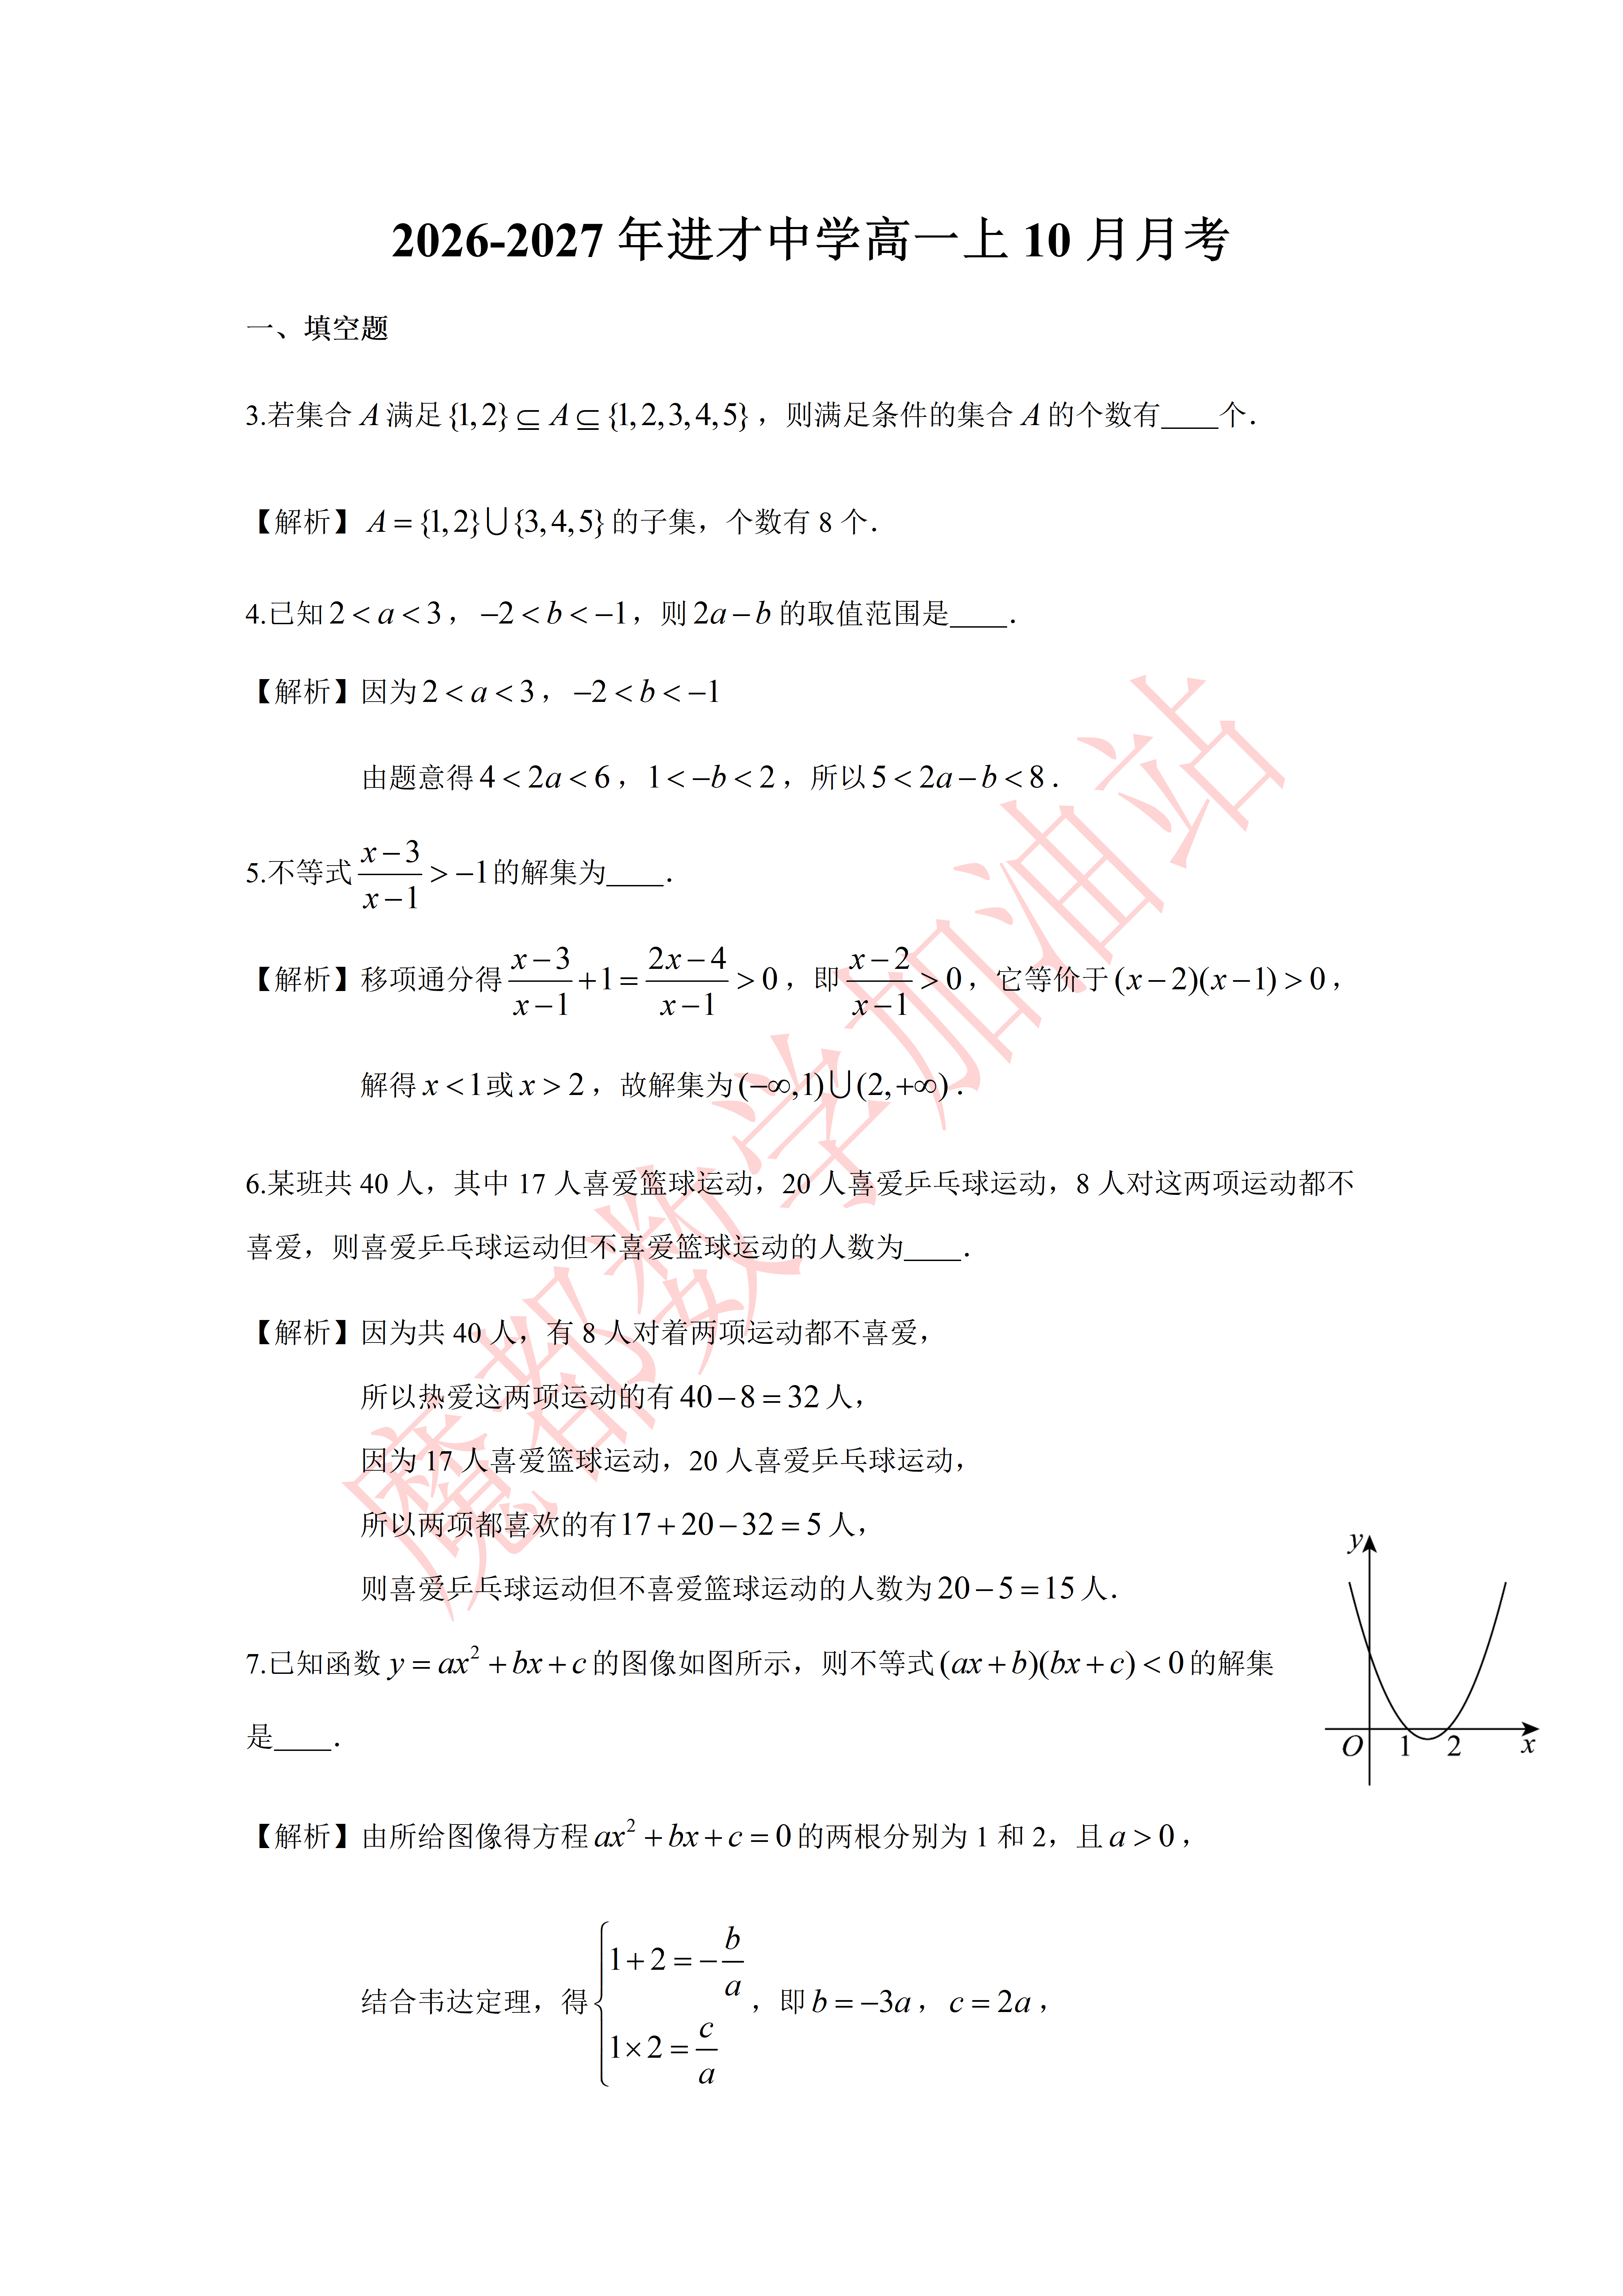
\includegraphics[width=.22\linewidth,trim=3879bp 1490bp 238bp 4492bp,clip]{../原图/高一60_进才中学_10月月考/01.png}
\end{center}

\ifanswer
\solbegin
\step{由所给图像得方程 $ax^2+bx+c=0$ 的两根分别为 1 和 2，且 $a>0$，}
\step{结合韦达定理，得 $\begin{cases}1+2=-\dfrac ba\\ 1\times2=\dfrac ca\end{cases}$，即 $b=-3a$，$c=2a$，}
\step{所以不等式 $(ax+b)(bx+c)<0$ 即 $(ax-3a)(-3ax+2a)<0$，}
\step{化简得 $(x-3)(3x-2)>0$，解得 $x<\dfrac23$ 或 $x>3$，}
\step{所以不等式 $(ax+b)(bx+c)<0$ 的解集是 $(-\infty,\dfrac23)\cup(3,+\infty)$.}
\solend
\fi

\item 已知集合 $A=\{x\mid ax=6\}$，满足 $A\subseteq\Z$，则整数 $a$ 的所有可能取值有\blankline[4.4em]个.

\ifanswer
\solbegin
\step{当 $a=0$ 时，$A=\varnothing$，而 $\varnothing\subseteq\Z$，满足题意，}
\step{当 $a\neq0$ 时，$A=\left\{\dfrac6a\right\}$，要使 $A\subseteq\Z$，则 $\dfrac6a\in\Z$，所以 $a=\pm1,\pm2,\pm3,\pm6$，}
\step{综上，整数 $a$ 的可能取值为 0，$\pm1$，$\pm2$，$\pm3$，$\pm6$，共 9 个.}
\solend
\fi

\item 设关于 $x$ 的方程 $x^2+kx+n=0$ 有两个不同实根 $x_1$、$x_2$，且 $\dfrac1{x_1}+\dfrac1{x_2}=2$，则实数 $n$ 的取值范围是\blankline[4.4em].

\ifanswer
\solbegin
\step{由于方程 $x^2+kx+n=0$ 有两个不同实根 $x_1$、$x_2$，}
\step{因此 $\Delta=k^2-4n>0$，$x_1+x_2=-k$，$x_1x_2=n$，}
\step{由 $\dfrac1{x_1}+\dfrac1{x_2}=\dfrac{x_1+x_2}{x_1x_2}=\dfrac{-k}{n}=2$，得 $k=-2n$，}
\step{因此 $\Delta=k^2-4n=4n^2-4n>0$，解得 $n<0$ 或 $n>1$，}
\step{则实数 $n$ 的取值范围是 $(-\infty,0)\cup(1,+\infty)$.}
\solend
\fi

\item 某船从甲地沿河顺流航行 $75\mathrm{km}$，到达乙码头，停留 $30\mathrm{min}$ 后再逆流航行 $126\mathrm{km}$ 到达丙地，若水流速度为 $4\mathrm{km/h}$，且该船要在 $5\mathrm{h}$ 内完成航行任务，那么船的速度至少达到\blankline[4.4em]$\mathrm{km/h}$.

\ifanswer
\solbegin
\step{设该轮船在静水中的速度是 $x$ 千米/小时，水流速度是 4 千米/小时，}
\step{由题意得 $\dfrac{75}{4+x}+0.5+\dfrac{126}{x-4}\leqslant5$，即 $9x^2-402x-552\geqslant0$，解得 $x\geqslant46$，}
\step{答：该船的速度至少是 46 千米/小时.}
\solend
\fi

\item 设实数 $a,b,c$ 满足 $a^2+b^2\leqslant c<1$，则 $a+\dfrac12b+c$ 的最小值为\blankline[4.4em].

\ifanswer
\solbegin
\step{因为 $c\geqslant a^2+b^2$，}
\step{所以 $a+\dfrac12b+c\geqslant a+\dfrac12b+a^2+b^2=\left(a+\dfrac12\right)^2+\left(b+\dfrac14\right)^2-\dfrac5{16}\geqslant-\dfrac5{16}$，}
\step{当 $a=-\dfrac12,b=-\dfrac14,c=a^2+b^2=\dfrac5{16}$（此时 $c<1$ 成立）时取到等号，}
\step{故最小值为 $-\dfrac5{16}$.}
\solend
\fi

\item 已知集合 $A=\{x\in\N^*\mid1\leqslant x\leqslant2026\}$. 设集合 $B=\{b_1,b_2,b_3,\cdots,b_n\}$ 满足 $B\subseteq A$，且对任意的 $b_i$、$b_j$、$b_k\in B(i$、$j$、$k\in\{1,2,3,\cdots,n\})$，存在 $m\in\N^*$，使得 $b_i+b_j+b_k=39m$，则 $n$ 的最大值为\blankline[4.4em].

\ifanswer
\solbegin
\step{因为 $39=1\times39=3\times13$，所以 $n$ 的最大值大于 3，}
\step{若对任意的 $b_i$、$b_j$、$b_k\in B$，存在 $m\in\N^*$，使得 $b_i+b_j+b_k=39m$，}
\step{则集合 $B$ 的元素除以 39 的余数均为 0 或均为 13 或均为 26，}
\step{即 $B=\{39,78,\cdots,39n\}$ 或 $B=\{13,52,\cdots,39n-26\}$}
\step{或 $B=\{26,65,\cdots,39n-13\}$，}
\step{若 $B=\{39,78,\cdots,39n\}$，则 $39n\leqslant2026$，}
\step{解得 $n\leqslant\dfrac{2026}{39}\in(51,52)$，此时 $n$ 的最大值为 51；}
\step{若 $B=\{13,52,\cdots,39n-26\}$，则 $39n-26\leqslant2026$，}
\step{解得 $n\leqslant\dfrac{684}{13}\in(52,53)$，此时 $n$ 的最大值为 52；}
\step{若 $B=\{26,65,\cdots,39n-13\}$，则 $39n-13\leqslant2026$，}
\step{解得 $n\leqslant\dfrac{2039}{39}\in(52,53)$，此时 $n$ 的最大值为 52；}
\step{综上，$n$ 的最大值为 52.}
\solend
\fi

\end{enumerate}

\bigsec{二、选择题}

\begin{enumerate}
\setcounter{enumi}{12}

% 第 13 题原卷无【答案】/【解析】段，答案“B”直接印在题干括号内，
% 按 高一53 第 13 题的成例括号留空、答案另提为 \ans{}（见文件头）
\item 已知 $a$、$b\in\R$，则“$|a|>|b|$”是“$a>|b|$”的\mbox{（\quad）}

\keepwithprev
A. 充分不必要条件\qquad B. 必要不充分条件

C. 充要条件\qquad D. 既不充分也不必要条件

\ifanswer
\ans{$B$}
\fi

\item 如果关于 $x$ 的一元二次方程 $x^2+2mx+(m+2)=0$ 有一正根一负根，那么 $m$ 的取值范围为\mbox{（\quad）}

\keepwithprev
A. $(-2,-1)$\qquad B. $(-1,2)$

C. $(-\infty,-1)\cup(2,+\infty)$\qquad D. $(-\infty,-2)$

\ifanswer
\solbegin
\step{设两根为 $x_1,x_2$，方程有一正根一负根，则 $\begin{cases}x_1x_2=m+2<0\\ \Delta=4m^2-4(m+2)>0\end{cases}$，}
\step{解得 $m<-2$，故选 $D$.}
\solend
\fi

\item 若不等式 $|3x-a|\leqslant x+2$ 的解集包含集合 $[0,1]$，则实数 $a$ 的取值范围为\mbox{（\quad）}

\keepwithprev
A. $[0,2]$\qquad B. $[0,1]$

C. $[1,2]$\qquad D. $(1,2)$

\ifanswer
\solbegin
% 原卷“法一：”“法二：”排红色加粗（全卷唯一红字），本稿按全稿子题标号样式排 \stepm
% （详见文件头“与原卷的排版差异”⑦）
\stepm{法一：}{不等式 $|3x-a|\leqslant x+2$ 化为 $2x-2\leqslant a\leqslant4x+2$，}
% 原卷此句缺动词（疑漏“对”字），照录未改（见文件头“原卷存疑”④）
\step{$[0,1]$ 使 $2x-2\leqslant a\leqslant4x+2$ 成立，则 $0\leqslant a\leqslant2$，故选 $A$.}
\stepm{法二：}{将两边平方整理得 $8x^2-(6a+4)x+a^2-4\leqslant0$ 对 $[0,1]$ 恒成立，}
\step{则有 $\begin{cases}a^2-4\leqslant0\\ a^2-6a\leqslant0\end{cases}$，解得 $0\leqslant a\leqslant2$，故选 $A$.}
\solend
\fi

\item 数学组 Y 老师在白纸上写下以下四个命题：

①这四个命题中至少有一个是真的；②这四个命题中至少有两个是真的；

③这四个命题中至少有两个是假的；④这四个命题中至少有一个是假的；

每个命题非真即假. 问 Y 老师在纸上写的假命题有几个？\mbox{（\quad）}

\keepwithprev
A. 0\qquad B. 1

C. 2\qquad D. 3

\ifanswer
\solbegin
\step{设四个命题中真命题的个数为 $t$，则①真 $\iff t\geqslant1$，②真 $\iff t\geqslant2$，}
\step{③真 $\iff t\leqslant2$，④真 $\iff t\leqslant3$.}
\step{逐一检验：$t=0$ 时③④为真，应为 $t=2$，矛盾；}
\step{$t=1$ 时①③④为真，应为 $t=3$，矛盾；}
\step{$t=2$ 时四个命题全为真，应为 $t=4$，矛盾；}
\step{$t=3$ 时①②④为真、③为假，恰有 3 个真命题，符合；}
\step{$t=4$ 时①②为真，应为 $t=2$，矛盾.}
\step{所以恰有 1 个假命题，故选 $B$.}
\solend
\fi

\end{enumerate}

\bigsec{三、解答题}

\begin{enumerate}
\setcounter{enumi}{16}

\item 已知：$x\in\R$，$a=x^2-1$，$b=4x+5$. 求证：$a$、$b$ 中至少有一个大于等于 0.

\ifanswer
\solbegin
\step{假设 $a$、$b$ 都小于 0，即 $a<0$，$b<0$，则 $a+b<0$.}
\step{又 $a+b=x^2-1+4x+5=x^2+4x+4=(x+2)^2\geqslant0$，}
\step{这与假设所得 $a+b<0$ 矛盾，故假设不成立，}
\step{所以 $a$、$b$ 中至少有一个大于等于 0.}
\solend
\fi

\ansspace[6]

% 原卷 A、B 两个集合定义之间排半角逗号“,”（5 倍放大核，右侧字距 19px，与全卷全角“，”的 65—79px 字距判然有别）；
% 本稿原误抄为全角“，”——已照录原卷半角（见文件头“与原卷的排版差异”⑤）
\item 已知集合 $A=\{x\mid4\leqslant x\leqslant12\}$,$B=\{x\mid a\leqslant x\leqslant2a+1\}$.

（1）若 $a=2$，求 $\overline A\cap B$；

（2）已知 $A\cup B=A$，求实数 $a$ 的取值范围.

\ifanswer
\solbegin
\stepm{(1)}{当 $a=2$ 时，$B=\{x\mid2\leqslant x\leqslant5\}$，}
\step{而 $A=\{x\mid4\leqslant x\leqslant12\}$，则 $\overline A=(-\infty,4)\cup(12,+\infty)$，所以 $\overline A\cap B=[2,4)$.}
\stepm{(2)}{$A\cup B=A$ 即 $B\subseteq A$.}
\stepm{①}{当 $B=\varnothing$ 时，$a>2a+1$，即 $a<-1$，符合；}
\stepm{②}{当 $B\neq\varnothing$ 时，需 $a\leqslant2a+1$ 且 $a\geqslant4$ 且 $2a+1\leqslant12$，即 $4\leqslant a\leqslant\dfrac{11}2$.}
\step{综上，$a$ 的取值范围是 $(-\infty,-1)\cup\left[4,\dfrac{11}2\right]$.}
\solend
\fi

\ansspace[8]

\item （1）若关于 $x$ 的不等式 $ax^2-3x+2<0$ 的解集不是空集，求实数 $a$ 的取值范围；

（2）求关于 $x$ 的不等式 $ax^2-3x+2>ax-1$ 的解集.

\ifanswer
\solbegin
\stepm{(1)}{若 $a>0$，关于 $x$ 的不等式 $ax^2-3x+2<0$ 的解集不空，}
\step{所以一元二次方程 $ax^2-3x+2=0$ 的判别式大于零，}
\step{即 $(-3)^2-8a>0\Rightarrow a<\dfrac98$，结合 $a>0$ 得 $0<a<\dfrac98$；}
\step{若 $a\leqslant0$，则关于 $x$ 的不等式 $ax^2-3x+2<0$ 的解集不是空集；}
\step{综上，实数 $a$ 的取值范围是 $\left(-\infty,\dfrac98\right)$.}
\stepm{(2)}{$ax^2-3x+2>ax-1\Rightarrow ax^2-(a+3)x+3>0\Rightarrow(ax-3)(x-1)>0$，}
\step{当 $a=0$ 时，不等式为 $x-1<0$，不等式的解集为 $\{x\mid x<1\}$；}
\step{当 $a<0$ 时，不等式化为 $\left(x-\dfrac3a\right)(x-1)<0$，}
\step{不等式的解集为 $\left\{x\mid\dfrac3a<x<1\right\}$，}
\step{当 $a>0$ 时，方程 $ax^2-3x+2=ax-1$ 的两个根分别为：$\dfrac3a,1$.}
\step{当 $a=3$ 时，两根相等，故不等式的解集为 $\{x\mid x\neq1\}$；}
\step{当 $a>3$ 时，$\dfrac3a<1$，不等式的解集为 $\left\{x\mid x<\dfrac3a\right.$ 或 $\left.x>1\right\}$；}
\step{当 $0<a<3$ 时，$\dfrac3a>1$，不等式的解集为 $\left\{x\mid x<1\right.$ 或 $\left.x>\dfrac3a\right\}$；}
\step{综上所述，当 $a<0$ 时，不等式的解集为 $\left\{x\mid\dfrac3a<x<1\right\}$，}
\step{当 $a=0$ 时，不等式的解集为 $\{x\mid x<1\}$，}
\step{当 $0<a<3$ 时，不等式的解集为 $\left\{x\mid x<1\right.$ 或 $\left.x>\dfrac3a\right\}$，}
\step{当 $a=3$ 时，不等式的解集为 $\{x\mid x\neq1\}$，}
\step{当 $a>3$ 时，不等式的解集为 $\left\{x\mid x<\dfrac3a\right.$ 或 $\left.x>1\right\}$.}
\solend
\fi

\ansspace[8]

\item 设命题 $p$：对任意 $x\in\R$，使得不等式 $mx^2-mx+2>0$ 恒成立；命题 $q$：存在 $0\leqslant x\leqslant3$，不等式 $2x-2\geqslant|m|$ 成立.

（1）若 $p$ 为真命题，求实数 $m$ 的取值范围；

（2）若 $p$、$q$ 有且只有一个是真命题，求实数 $m$ 的取值范围.

\ifanswer
\solbegin
\stepm{(1)}{因为 $p:\forall x\in\R$，$mx^2-mx+2>0$ 为真命题，}
\step{所以当 $m=0$ 时，不等式为 $2>0$，在 $\R$ 上恒成立，符合题意；}
\step{当 $m\neq0$ 时，$\begin{cases}m>0\\ \Delta=m^2-8m<0\end{cases}$，解得 $0<m<8$.}
\step{综上，实数 $m$ 的取值范围为 $[0,8)$.}
\stepm{(2)}{若 $q$ 为真命题，即 $q:\exists0\leqslant x\leqslant3$，$2x-2\geqslant|m|$，}
\step{则对于 $0\leqslant x\leqslant3$，$(2x-2)_{max}\geqslant|m|$.}
\step{由于 $0\leqslant x\leqslant3$，$2x-2\in[-2,4]$，所以 $|m|\leqslant4$，解得 $-4\leqslant m\leqslant4$，}
\step{又因为 $p$、$q$ 有且只有一个是真命题，}
\step{所以当 $p$ 真 $q$ 假时，$\begin{cases}0\leqslant m<8\\ m<-4\text{或}m>4\end{cases}$，解得 $4<m<8$；}
\step{当 $p$ 假 $q$ 真时，$\begin{cases}m<0\text{或}m\geqslant8\\ -4\leqslant m\leqslant4\end{cases}$，解得 $-4\leqslant m<0$；}
\step{综上，实数 $m$ 的取值范围为 $[-4,0)\cup(4,8)$.}
\solend
\fi

\ansspace[10]

\item 已知集合 $A=\{a_1,a_2,\cdots,a_k\}(k\geqslant2)$. 其中 $a_i\in\N^*(i=1,2,\cdots,k)$. 若对于任意的 $a\in A$，总有 $\dfrac1a\notin A$，则称集合 $A$ 具有性质 $P$. 由 $A$ 中的元素构成两个相应的集合：$S=\{(a,b)\mid a\in A,b\in A,ab\in A\}$，$T=\left\{(a,b)\mid a\in A,b\in A,\dfrac ab\in A\right\}$，其中 $(a,b)$ 是有序数对，集合 $S$ 和 $T$ 中的元素个数分别为 $m$ 和 $n$.

（1）检验集合 $\{2,3,6\}$ 与 $\{1,2,4\}$ 是否具有性质 $P$，并对其中具有性质 $P$ 的集合，写出相应的集合 $S$ 和 $T$；

（2）对任何具有性质 $P$ 的集合 $A$，$n$ 的最大值为多少？（直接写出答案，无需说明理由）；

% 原卷题干的小问编号跳号：印作 (1)(2)(4)，本稿照录 (4)、未改成 (3)（见文件头“原卷存疑”①）
（4）判断 $m$ 和 $n$ 的大小关系，并证明你的结论.

\ifanswer
\solbegin
\stepm{(1)}{因为 $\dfrac12\in\{1,2,4\}$，所以 $\{1,2,4\}$ 不具有性质 $P$；}
\step{因为 $\dfrac12\notin\{2,3,6\}$，$\dfrac13\notin\{2,3,6\}$，$\dfrac16\notin\{2,3,6\}$，所以 $\{2,3,6\}$ 具有性质 $P$.}
\step{$S=\{(2,3),(3,2)\}$，$T=\{(6,2),(6,3)\}$；}
\stepm{(2)}{因为对于任意的 $a\in A$，总有 $\dfrac1a\notin A$，所以 $1\notin A$，}
% 原卷此处印作“$\{(a_i,a_i)\}\in T$”，与上一句“$1\notin A$”及下文“最多为 $C_k^2$”的推理
% 均不自洽（应为“$\notin$”），已 8 倍放大确认无斜线；照录未改（见文件头“原卷存疑”③）
\step{从而 $\{(a_i,a_i)\}\in T(i=1,2,\cdots,k)$.}
\step{因为 $a\in A,b\in A,\dfrac ab\in A$，所以当 $i\neq j$ 时，}
\step{$(a_i,a_j)\in T$ 和 $(a_j,a_i)\in T(i,j=1,2,\cdots,k)$ 至多有一个成立，}
\step{所以集合 $T$ 中的元素个数最多为 $C_k^2=\dfrac{k(k-1)}2$，即 $n\leqslant\dfrac{k(k-1)}2$.}
% 原卷【解析】把第 (4) 问标作“(3)”（与题干跳号相应），本稿照录未改（见文件头“原卷存疑”①）
\stepm{(3)}{$m=n$，证明如下：}
\step{①设 $(a,b)\in T$，则 $a\in A,b\in A,\dfrac ab\in A$. 设 $c=\dfrac ab$，则 $a=bc$，}
\step{故 $b\in A$，$c\in A$，$bc\in A$，从而 $(b,c)\in S$，}
\step{即对 $\forall(a,b)\in T$，总 $\exists c$ 使 $(b,c)\in S$，从而 $n\leqslant m$.}
\step{②设 $(p,q)\in S$，则 $p\in A$，$q\in A$，$pq\in A$.}
\step{设 $r=pq$，则 $q=\dfrac rp$，故 $r\in A,p\in A,\dfrac rp\in A$，从而 $(r,p)\in T$，}
\step{即对 $\forall(p,q)\in S$，总 $\exists r$ 使 $(r,p)\in T$，从而 $m\leqslant n$.}
\step{由①②得 $m=n$.}
\solend
\fi

\ansspace*[10]

\end{enumerate}

\end{document}
"
% 紧凑版：xelatex "\def\iscompact{1}% 高一60_进才中学_10月月考.tex
%   —— 高一上数学“2026-2027 年进才中学高一上 10 月月考”（讲评版）
% 试卷版：xelatex 高一60_进才中学_10月月考.tex
% 答案版：xelatex "\def\isanswer{1}\input{高一60_进才中学_10月月考.tex}"
% 紧凑版：xelatex "\def\iscompact{1}\input{高一60_进才中学_10月月考.tex}"
%
% 原文链接：https://mp.weixin.qq.com/s/2ZLKB3IONEDhcUAfAAYE2A。
% 公众号“魔都数学加油站”作者破晓于 2026-10-14 22:15 发布。
% 原图 9 张（`原图/高一60_进才中学_10月月考/01..09.png`）：第 1—8 页 4762×6735，
% 第 9 页 2560×3620（同一篇内两档分辨率）。
%
% 卷首标题：照卷面印作“2026--2027 年进才中学高一上 10 月月考”（公众号标题中的“上海市”
% 卷面标题行没有，本稿照卷面），年份区间按全稿惯例排 en dash。原卷只有一行标题、无副标题。
%
% 篇幅与题号：原卷自第 3 题起编号（第 1、2 题不在本卷内）。填空题 3—12（10 题）、
% 选择题 13—16（4 题）、解答题 17—21（5 题），共 19 题。本稿沿用原节与原题号，
% 只改排为全稿统一的大节样式（原卷小节标题为“一、填空题”“二、选择题”“三、解答题”）。
%
% 讲评版：原卷每题下直接印【答案】或【解析】。**只印【解析】的 18 题**，本稿按全稿口径
% 收进答案版、不另提 \ans{}——第 14、15、16 题的结论写在解析末句（“故选 D／A／B”），
% 亦照录在解析内。**第 13 题原卷没有任何【答案】/【解析】段**，答案“B”直接印在题干括号内
% （“（ B ）”），本稿按 高一53 第 13 题的成例把括号留空、答案另提为 \ans{$B$}（见下）。
%
% 副标题：原卷未印副标题。本稿按“知识模块”口径标作“集合与常用逻辑用语、不等式”：
% 19 题中集合与常用逻辑用语 10 题（第 3、6、8、12、13、16、17、18、20、21 题，
% 含子集计数、韦恩图容斥、集合运算、命题与充要条件、反证法、新定义），
% 不等式 9 题（含不等式性质、分式不等式、二次函数与解集、韦达定理与判别式、
% 不等式应用、最值、根的分布、绝对值不等式恒成立、含参二次不等式：第 4、5、7、9、10、
% 11、14、15、19 题），两类均远超三分之一，故并标。口径同 高一46、高一47、高一48、
% 高一51—高一59。
%
% 与原卷的排版差异：
%   ① 原卷每题下直接印【答案】/【解析】，本稿按全稿惯例将答案与解析置于答案版，试卷版保持干净；
%   ② 原卷未印副标题，本稿按“知识模块”口径补出；
%   ③ 原卷填空横线约两个字宽，本稿按全稿惯例统一排 \blankline[4.4em]；
%   ④ 原卷实数集排斜体 $R$（第 13、17、20 题）、正整数集排 $N^*$（第 12、21 题）、
%      整数集排粗体 $\mathbf{Z}$（第 8 题），本稿按全稿惯例改用 $\R$、$\N^*$、$\Z$；
%      空集记号统一为 \varnothing；
%   ⑤ 原卷在数学式内多处用半角逗号（如 $x_1,x_2$、$a,b\in R$，以及第 18 题题干
%      $A=\{x\mid4\leqslant x\leqslant12\}$,$B=\{x\mid a\leqslant x\leqslant2a+1\}$ 之间的逗号），
%      均照录未强改（第 18 题题干那一处本稿首轮曾误作全角“，”，第二轮已订正）；
%      句末句点按全稿惯例排西文句点；
%   ⑥ 第 13 题印在题干括号内的答案“B”移入 \ans{}，见上；
%   ⑦ 第 15 题【解析】的“法一：”“法二：”标号原卷排**红色加粗**（全卷唯一的红字，2 处），
%      本稿按全稿子题标号样式排 \stepm{法一：}{…}、\stepm{法二：}{…}（加粗着色、不改黑色
%      基调），冒号照原卷排全角；
%   ⑧ 第 7 题的图像原卷排在题干右侧（与题干第 1 行同高），本稿居中排在题干之后；
%      图自原图第 01 页裁切（trim），不另存图片文件；
%   ⑨ 原卷第 10 题的长度与速度单位原卷排斜体（$75km$、$4km/h$ 等），本稿按全稿惯例
%      改排正体 $\mathrm{km}$、$\mathrm{km/h}$（同 高一56 第 13 题）；每道解答题原卷未留
%      作答空白，本稿按全稿惯例加 \ansspace。
%
% 原卷存疑（照录未改，见源码中该处上方注释）：
%   ① 第 21 题题干的小问编号**跳号**：印作 (1)(2)(4)，而紧随其后的【解析】按 (1)(2)(3) 写
%      —— 题干第 (4) 问实为第 (3) 问。本稿题干照录 (1)(2)(4)、解析照录 (3)，未改
%      （与 高一22 第 16 题“解析误标 (2)”同一处理）。
%   ② 第 6 题【解析】“有 8 人**对着**两项运动都不喜爱”，“对着”疑为“对这”之误，照录未改。
%   ③ 第 21(2) 题【解析】首行“所以 $1\notin A$，从而 $\{(a_i,a_i)\}\in T(i=1,2,\cdots,k)$”
%      —— 由 $1\notin A$ 应得 $(a_i,a_i)\notin T$（因 $a_i/a_i=1$），与紧随的“$T$ 中元素
%      个数最多为 $C_k^2$”这一推理亦只有“$\notin$”才自洽；原卷此处印作“$\in$”，
%      已 8 倍放大确认无斜线。**照录原卷的 $\in$、未改**。
%   ④ 第 15 题【解析】法一“$[0,1]$ 使 $2x-2\leqslant a\leqslant4x+2$ 成立”一句缺动词
%      （疑漏“对”字），照录未改。
%
\documentclass[a4paper,11pt]{article}
\usepackage{common}

\begin{document}

\examtitlest[3]{2026--2027 年进才中学高一上 10 月月考}{集合与常用逻辑用语、不等式}

\bigsec{一、填空题}

\begin{enumerate}
\setcounter{enumi}{2}

\item 若集合 $A$ 满足 $\{1,2\}\subseteq A\subseteq\{1,2,3,4,5\}$，则满足条件的集合 $A$ 的个数有\blankline[4.4em]个.

\ifanswer
\solbegin
\step{$A=\{1,2\}\cup\{3,4,5\}$ 的子集，个数有 8 个.}
\solend
\fi

\item 已知 $2<a<3$，$-2<b<-1$，则 $2a-b$ 的取值范围是\blankline[4.4em].

\ifanswer
\solbegin
\step{因为 $2<a<3$，$-2<b<-1$，}
\step{由题意得 $4<2a<6$，$1<-b<2$，所以 $5<2a-b<8$.}
\solend
\fi

\item 不等式 $\dfrac{x-3}{x-1}>-1$ 的解集为\blankline[4.4em].

\ifanswer
\solbegin
\step{移项通分得 $\dfrac{x-3}{x-1}+1=\dfrac{2x-4}{x-1}>0$，即 $\dfrac{x-2}{x-1}>0$，它等价于 $(x-2)(x-1)>0$，}
\step{解得 $x<1$ 或 $x>2$，故解集为 $(-\infty,1)\cup(2,+\infty)$.}
\solend
\fi

\item 某班共 40 人，其中 17 人喜爱篮球运动，20 人喜爱乒乓球运动，8 人对这两项运动都不喜爱，则喜爱乒乓球运动但不喜爱篮球运动的人数为\blankline[4.4em].

\ifanswer
\solbegin
% 原卷作“对着两项运动都不喜爱”（疑为“对这”之误），照录未改（见文件头“原卷存疑”②）
\step{因为共 40 人，有 8 人对着两项运动都不喜爱，}
\step{所以热爱这两项运动的有 $40-8=32$ 人，}
\step{因为 17 人喜爱篮球运动，20 人喜爱乒乓球运动，}
\step{所以两项都喜欢的有 $17+20-32=5$ 人，}
\step{则喜爱乒乓球运动但不喜爱篮球运动的人数为 $20-5=15$ 人.}
\solend
\fi

\item 已知函数 $y=ax^2+bx+c$ 的图像如图所示，则不等式 $(ax+b)(bx+c)<0$ 的解集是\blankline[4.4em].

% 原图第 01 页题干右侧的图像直接裁取。裁框取图外框 x 3887–4516、y 4500–5237
% （四周各留约 8px），trim=左 3879bp／下 1490bp／右 238bp／上 4492bp
% （页宽 4762、页高 6735）。
\begin{center}
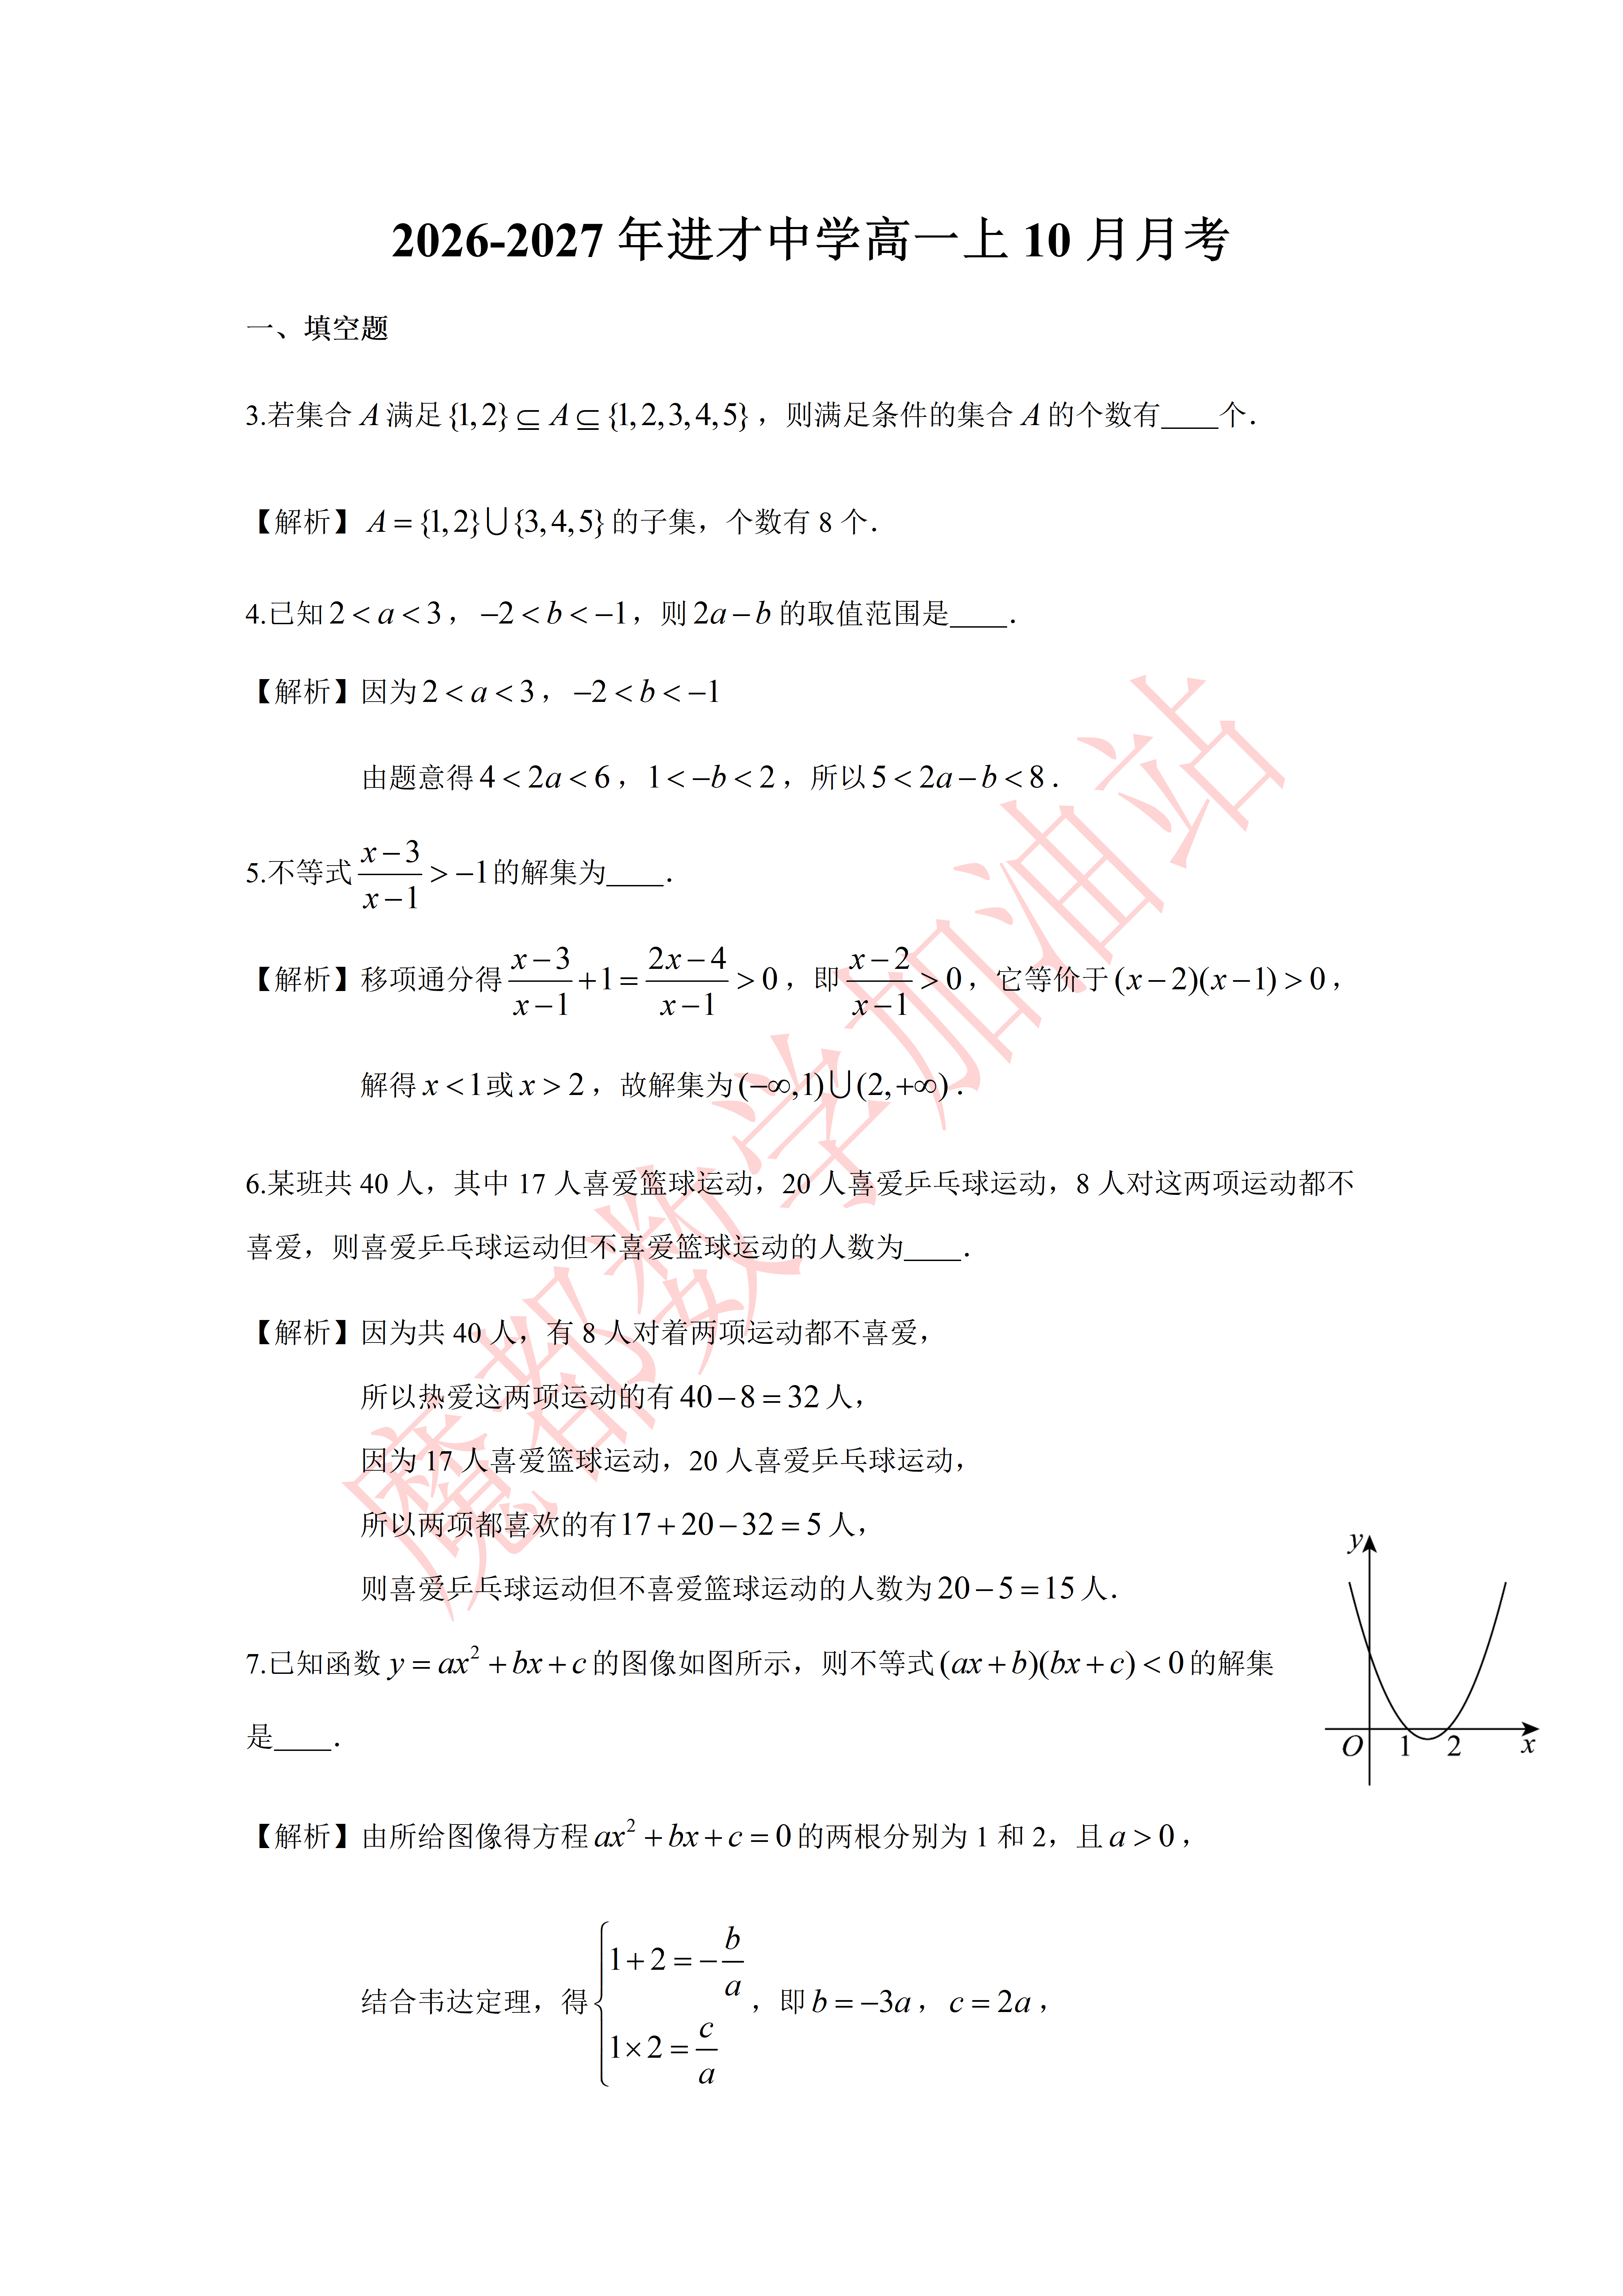
\includegraphics[width=.22\linewidth,trim=3879bp 1490bp 238bp 4492bp,clip]{../原图/高一60_进才中学_10月月考/01.png}
\end{center}

\ifanswer
\solbegin
\step{由所给图像得方程 $ax^2+bx+c=0$ 的两根分别为 1 和 2，且 $a>0$，}
\step{结合韦达定理，得 $\begin{cases}1+2=-\dfrac ba\\ 1\times2=\dfrac ca\end{cases}$，即 $b=-3a$，$c=2a$，}
\step{所以不等式 $(ax+b)(bx+c)<0$ 即 $(ax-3a)(-3ax+2a)<0$，}
\step{化简得 $(x-3)(3x-2)>0$，解得 $x<\dfrac23$ 或 $x>3$，}
\step{所以不等式 $(ax+b)(bx+c)<0$ 的解集是 $(-\infty,\dfrac23)\cup(3,+\infty)$.}
\solend
\fi

\item 已知集合 $A=\{x\mid ax=6\}$，满足 $A\subseteq\Z$，则整数 $a$ 的所有可能取值有\blankline[4.4em]个.

\ifanswer
\solbegin
\step{当 $a=0$ 时，$A=\varnothing$，而 $\varnothing\subseteq\Z$，满足题意，}
\step{当 $a\neq0$ 时，$A=\left\{\dfrac6a\right\}$，要使 $A\subseteq\Z$，则 $\dfrac6a\in\Z$，所以 $a=\pm1,\pm2,\pm3,\pm6$，}
\step{综上，整数 $a$ 的可能取值为 0，$\pm1$，$\pm2$，$\pm3$，$\pm6$，共 9 个.}
\solend
\fi

\item 设关于 $x$ 的方程 $x^2+kx+n=0$ 有两个不同实根 $x_1$、$x_2$，且 $\dfrac1{x_1}+\dfrac1{x_2}=2$，则实数 $n$ 的取值范围是\blankline[4.4em].

\ifanswer
\solbegin
\step{由于方程 $x^2+kx+n=0$ 有两个不同实根 $x_1$、$x_2$，}
\step{因此 $\Delta=k^2-4n>0$，$x_1+x_2=-k$，$x_1x_2=n$，}
\step{由 $\dfrac1{x_1}+\dfrac1{x_2}=\dfrac{x_1+x_2}{x_1x_2}=\dfrac{-k}{n}=2$，得 $k=-2n$，}
\step{因此 $\Delta=k^2-4n=4n^2-4n>0$，解得 $n<0$ 或 $n>1$，}
\step{则实数 $n$ 的取值范围是 $(-\infty,0)\cup(1,+\infty)$.}
\solend
\fi

\item 某船从甲地沿河顺流航行 $75\mathrm{km}$，到达乙码头，停留 $30\mathrm{min}$ 后再逆流航行 $126\mathrm{km}$ 到达丙地，若水流速度为 $4\mathrm{km/h}$，且该船要在 $5\mathrm{h}$ 内完成航行任务，那么船的速度至少达到\blankline[4.4em]$\mathrm{km/h}$.

\ifanswer
\solbegin
\step{设该轮船在静水中的速度是 $x$ 千米/小时，水流速度是 4 千米/小时，}
\step{由题意得 $\dfrac{75}{4+x}+0.5+\dfrac{126}{x-4}\leqslant5$，即 $9x^2-402x-552\geqslant0$，解得 $x\geqslant46$，}
\step{答：该船的速度至少是 46 千米/小时.}
\solend
\fi

\item 设实数 $a,b,c$ 满足 $a^2+b^2\leqslant c<1$，则 $a+\dfrac12b+c$ 的最小值为\blankline[4.4em].

\ifanswer
\solbegin
\step{因为 $c\geqslant a^2+b^2$，}
\step{所以 $a+\dfrac12b+c\geqslant a+\dfrac12b+a^2+b^2=\left(a+\dfrac12\right)^2+\left(b+\dfrac14\right)^2-\dfrac5{16}\geqslant-\dfrac5{16}$，}
\step{当 $a=-\dfrac12,b=-\dfrac14,c=a^2+b^2=\dfrac5{16}$（此时 $c<1$ 成立）时取到等号，}
\step{故最小值为 $-\dfrac5{16}$.}
\solend
\fi

\item 已知集合 $A=\{x\in\N^*\mid1\leqslant x\leqslant2026\}$. 设集合 $B=\{b_1,b_2,b_3,\cdots,b_n\}$ 满足 $B\subseteq A$，且对任意的 $b_i$、$b_j$、$b_k\in B(i$、$j$、$k\in\{1,2,3,\cdots,n\})$，存在 $m\in\N^*$，使得 $b_i+b_j+b_k=39m$，则 $n$ 的最大值为\blankline[4.4em].

\ifanswer
\solbegin
\step{因为 $39=1\times39=3\times13$，所以 $n$ 的最大值大于 3，}
\step{若对任意的 $b_i$、$b_j$、$b_k\in B$，存在 $m\in\N^*$，使得 $b_i+b_j+b_k=39m$，}
\step{则集合 $B$ 的元素除以 39 的余数均为 0 或均为 13 或均为 26，}
\step{即 $B=\{39,78,\cdots,39n\}$ 或 $B=\{13,52,\cdots,39n-26\}$}
\step{或 $B=\{26,65,\cdots,39n-13\}$，}
\step{若 $B=\{39,78,\cdots,39n\}$，则 $39n\leqslant2026$，}
\step{解得 $n\leqslant\dfrac{2026}{39}\in(51,52)$，此时 $n$ 的最大值为 51；}
\step{若 $B=\{13,52,\cdots,39n-26\}$，则 $39n-26\leqslant2026$，}
\step{解得 $n\leqslant\dfrac{684}{13}\in(52,53)$，此时 $n$ 的最大值为 52；}
\step{若 $B=\{26,65,\cdots,39n-13\}$，则 $39n-13\leqslant2026$，}
\step{解得 $n\leqslant\dfrac{2039}{39}\in(52,53)$，此时 $n$ 的最大值为 52；}
\step{综上，$n$ 的最大值为 52.}
\solend
\fi

\end{enumerate}

\bigsec{二、选择题}

\begin{enumerate}
\setcounter{enumi}{12}

% 第 13 题原卷无【答案】/【解析】段，答案“B”直接印在题干括号内，
% 按 高一53 第 13 题的成例括号留空、答案另提为 \ans{}（见文件头）
\item 已知 $a$、$b\in\R$，则“$|a|>|b|$”是“$a>|b|$”的\mbox{（\quad）}

\keepwithprev
A. 充分不必要条件\qquad B. 必要不充分条件

C. 充要条件\qquad D. 既不充分也不必要条件

\ifanswer
\ans{$B$}
\fi

\item 如果关于 $x$ 的一元二次方程 $x^2+2mx+(m+2)=0$ 有一正根一负根，那么 $m$ 的取值范围为\mbox{（\quad）}

\keepwithprev
A. $(-2,-1)$\qquad B. $(-1,2)$

C. $(-\infty,-1)\cup(2,+\infty)$\qquad D. $(-\infty,-2)$

\ifanswer
\solbegin
\step{设两根为 $x_1,x_2$，方程有一正根一负根，则 $\begin{cases}x_1x_2=m+2<0\\ \Delta=4m^2-4(m+2)>0\end{cases}$，}
\step{解得 $m<-2$，故选 $D$.}
\solend
\fi

\item 若不等式 $|3x-a|\leqslant x+2$ 的解集包含集合 $[0,1]$，则实数 $a$ 的取值范围为\mbox{（\quad）}

\keepwithprev
A. $[0,2]$\qquad B. $[0,1]$

C. $[1,2]$\qquad D. $(1,2)$

\ifanswer
\solbegin
% 原卷“法一：”“法二：”排红色加粗（全卷唯一红字），本稿按全稿子题标号样式排 \stepm
% （详见文件头“与原卷的排版差异”⑦）
\stepm{法一：}{不等式 $|3x-a|\leqslant x+2$ 化为 $2x-2\leqslant a\leqslant4x+2$，}
% 原卷此句缺动词（疑漏“对”字），照录未改（见文件头“原卷存疑”④）
\step{$[0,1]$ 使 $2x-2\leqslant a\leqslant4x+2$ 成立，则 $0\leqslant a\leqslant2$，故选 $A$.}
\stepm{法二：}{将两边平方整理得 $8x^2-(6a+4)x+a^2-4\leqslant0$ 对 $[0,1]$ 恒成立，}
\step{则有 $\begin{cases}a^2-4\leqslant0\\ a^2-6a\leqslant0\end{cases}$，解得 $0\leqslant a\leqslant2$，故选 $A$.}
\solend
\fi

\item 数学组 Y 老师在白纸上写下以下四个命题：

①这四个命题中至少有一个是真的；②这四个命题中至少有两个是真的；

③这四个命题中至少有两个是假的；④这四个命题中至少有一个是假的；

每个命题非真即假. 问 Y 老师在纸上写的假命题有几个？\mbox{（\quad）}

\keepwithprev
A. 0\qquad B. 1

C. 2\qquad D. 3

\ifanswer
\solbegin
\step{设四个命题中真命题的个数为 $t$，则①真 $\iff t\geqslant1$，②真 $\iff t\geqslant2$，}
\step{③真 $\iff t\leqslant2$，④真 $\iff t\leqslant3$.}
\step{逐一检验：$t=0$ 时③④为真，应为 $t=2$，矛盾；}
\step{$t=1$ 时①③④为真，应为 $t=3$，矛盾；}
\step{$t=2$ 时四个命题全为真，应为 $t=4$，矛盾；}
\step{$t=3$ 时①②④为真、③为假，恰有 3 个真命题，符合；}
\step{$t=4$ 时①②为真，应为 $t=2$，矛盾.}
\step{所以恰有 1 个假命题，故选 $B$.}
\solend
\fi

\end{enumerate}

\bigsec{三、解答题}

\begin{enumerate}
\setcounter{enumi}{16}

\item 已知：$x\in\R$，$a=x^2-1$，$b=4x+5$. 求证：$a$、$b$ 中至少有一个大于等于 0.

\ifanswer
\solbegin
\step{假设 $a$、$b$ 都小于 0，即 $a<0$，$b<0$，则 $a+b<0$.}
\step{又 $a+b=x^2-1+4x+5=x^2+4x+4=(x+2)^2\geqslant0$，}
\step{这与假设所得 $a+b<0$ 矛盾，故假设不成立，}
\step{所以 $a$、$b$ 中至少有一个大于等于 0.}
\solend
\fi

\ansspace[6]

% 原卷 A、B 两个集合定义之间排半角逗号“,”（5 倍放大核，右侧字距 19px，与全卷全角“，”的 65—79px 字距判然有别）；
% 本稿原误抄为全角“，”——已照录原卷半角（见文件头“与原卷的排版差异”⑤）
\item 已知集合 $A=\{x\mid4\leqslant x\leqslant12\}$,$B=\{x\mid a\leqslant x\leqslant2a+1\}$.

（1）若 $a=2$，求 $\overline A\cap B$；

（2）已知 $A\cup B=A$，求实数 $a$ 的取值范围.

\ifanswer
\solbegin
\stepm{(1)}{当 $a=2$ 时，$B=\{x\mid2\leqslant x\leqslant5\}$，}
\step{而 $A=\{x\mid4\leqslant x\leqslant12\}$，则 $\overline A=(-\infty,4)\cup(12,+\infty)$，所以 $\overline A\cap B=[2,4)$.}
\stepm{(2)}{$A\cup B=A$ 即 $B\subseteq A$.}
\stepm{①}{当 $B=\varnothing$ 时，$a>2a+1$，即 $a<-1$，符合；}
\stepm{②}{当 $B\neq\varnothing$ 时，需 $a\leqslant2a+1$ 且 $a\geqslant4$ 且 $2a+1\leqslant12$，即 $4\leqslant a\leqslant\dfrac{11}2$.}
\step{综上，$a$ 的取值范围是 $(-\infty,-1)\cup\left[4,\dfrac{11}2\right]$.}
\solend
\fi

\ansspace[8]

\item （1）若关于 $x$ 的不等式 $ax^2-3x+2<0$ 的解集不是空集，求实数 $a$ 的取值范围；

（2）求关于 $x$ 的不等式 $ax^2-3x+2>ax-1$ 的解集.

\ifanswer
\solbegin
\stepm{(1)}{若 $a>0$，关于 $x$ 的不等式 $ax^2-3x+2<0$ 的解集不空，}
\step{所以一元二次方程 $ax^2-3x+2=0$ 的判别式大于零，}
\step{即 $(-3)^2-8a>0\Rightarrow a<\dfrac98$，结合 $a>0$ 得 $0<a<\dfrac98$；}
\step{若 $a\leqslant0$，则关于 $x$ 的不等式 $ax^2-3x+2<0$ 的解集不是空集；}
\step{综上，实数 $a$ 的取值范围是 $\left(-\infty,\dfrac98\right)$.}
\stepm{(2)}{$ax^2-3x+2>ax-1\Rightarrow ax^2-(a+3)x+3>0\Rightarrow(ax-3)(x-1)>0$，}
\step{当 $a=0$ 时，不等式为 $x-1<0$，不等式的解集为 $\{x\mid x<1\}$；}
\step{当 $a<0$ 时，不等式化为 $\left(x-\dfrac3a\right)(x-1)<0$，}
\step{不等式的解集为 $\left\{x\mid\dfrac3a<x<1\right\}$，}
\step{当 $a>0$ 时，方程 $ax^2-3x+2=ax-1$ 的两个根分别为：$\dfrac3a,1$.}
\step{当 $a=3$ 时，两根相等，故不等式的解集为 $\{x\mid x\neq1\}$；}
\step{当 $a>3$ 时，$\dfrac3a<1$，不等式的解集为 $\left\{x\mid x<\dfrac3a\right.$ 或 $\left.x>1\right\}$；}
\step{当 $0<a<3$ 时，$\dfrac3a>1$，不等式的解集为 $\left\{x\mid x<1\right.$ 或 $\left.x>\dfrac3a\right\}$；}
\step{综上所述，当 $a<0$ 时，不等式的解集为 $\left\{x\mid\dfrac3a<x<1\right\}$，}
\step{当 $a=0$ 时，不等式的解集为 $\{x\mid x<1\}$，}
\step{当 $0<a<3$ 时，不等式的解集为 $\left\{x\mid x<1\right.$ 或 $\left.x>\dfrac3a\right\}$，}
\step{当 $a=3$ 时，不等式的解集为 $\{x\mid x\neq1\}$，}
\step{当 $a>3$ 时，不等式的解集为 $\left\{x\mid x<\dfrac3a\right.$ 或 $\left.x>1\right\}$.}
\solend
\fi

\ansspace[8]

\item 设命题 $p$：对任意 $x\in\R$，使得不等式 $mx^2-mx+2>0$ 恒成立；命题 $q$：存在 $0\leqslant x\leqslant3$，不等式 $2x-2\geqslant|m|$ 成立.

（1）若 $p$ 为真命题，求实数 $m$ 的取值范围；

（2）若 $p$、$q$ 有且只有一个是真命题，求实数 $m$ 的取值范围.

\ifanswer
\solbegin
\stepm{(1)}{因为 $p:\forall x\in\R$，$mx^2-mx+2>0$ 为真命题，}
\step{所以当 $m=0$ 时，不等式为 $2>0$，在 $\R$ 上恒成立，符合题意；}
\step{当 $m\neq0$ 时，$\begin{cases}m>0\\ \Delta=m^2-8m<0\end{cases}$，解得 $0<m<8$.}
\step{综上，实数 $m$ 的取值范围为 $[0,8)$.}
\stepm{(2)}{若 $q$ 为真命题，即 $q:\exists0\leqslant x\leqslant3$，$2x-2\geqslant|m|$，}
\step{则对于 $0\leqslant x\leqslant3$，$(2x-2)_{max}\geqslant|m|$.}
\step{由于 $0\leqslant x\leqslant3$，$2x-2\in[-2,4]$，所以 $|m|\leqslant4$，解得 $-4\leqslant m\leqslant4$，}
\step{又因为 $p$、$q$ 有且只有一个是真命题，}
\step{所以当 $p$ 真 $q$ 假时，$\begin{cases}0\leqslant m<8\\ m<-4\text{或}m>4\end{cases}$，解得 $4<m<8$；}
\step{当 $p$ 假 $q$ 真时，$\begin{cases}m<0\text{或}m\geqslant8\\ -4\leqslant m\leqslant4\end{cases}$，解得 $-4\leqslant m<0$；}
\step{综上，实数 $m$ 的取值范围为 $[-4,0)\cup(4,8)$.}
\solend
\fi

\ansspace[10]

\item 已知集合 $A=\{a_1,a_2,\cdots,a_k\}(k\geqslant2)$. 其中 $a_i\in\N^*(i=1,2,\cdots,k)$. 若对于任意的 $a\in A$，总有 $\dfrac1a\notin A$，则称集合 $A$ 具有性质 $P$. 由 $A$ 中的元素构成两个相应的集合：$S=\{(a,b)\mid a\in A,b\in A,ab\in A\}$，$T=\left\{(a,b)\mid a\in A,b\in A,\dfrac ab\in A\right\}$，其中 $(a,b)$ 是有序数对，集合 $S$ 和 $T$ 中的元素个数分别为 $m$ 和 $n$.

（1）检验集合 $\{2,3,6\}$ 与 $\{1,2,4\}$ 是否具有性质 $P$，并对其中具有性质 $P$ 的集合，写出相应的集合 $S$ 和 $T$；

（2）对任何具有性质 $P$ 的集合 $A$，$n$ 的最大值为多少？（直接写出答案，无需说明理由）；

% 原卷题干的小问编号跳号：印作 (1)(2)(4)，本稿照录 (4)、未改成 (3)（见文件头“原卷存疑”①）
（4）判断 $m$ 和 $n$ 的大小关系，并证明你的结论.

\ifanswer
\solbegin
\stepm{(1)}{因为 $\dfrac12\in\{1,2,4\}$，所以 $\{1,2,4\}$ 不具有性质 $P$；}
\step{因为 $\dfrac12\notin\{2,3,6\}$，$\dfrac13\notin\{2,3,6\}$，$\dfrac16\notin\{2,3,6\}$，所以 $\{2,3,6\}$ 具有性质 $P$.}
\step{$S=\{(2,3),(3,2)\}$，$T=\{(6,2),(6,3)\}$；}
\stepm{(2)}{因为对于任意的 $a\in A$，总有 $\dfrac1a\notin A$，所以 $1\notin A$，}
% 原卷此处印作“$\{(a_i,a_i)\}\in T$”，与上一句“$1\notin A$”及下文“最多为 $C_k^2$”的推理
% 均不自洽（应为“$\notin$”），已 8 倍放大确认无斜线；照录未改（见文件头“原卷存疑”③）
\step{从而 $\{(a_i,a_i)\}\in T(i=1,2,\cdots,k)$.}
\step{因为 $a\in A,b\in A,\dfrac ab\in A$，所以当 $i\neq j$ 时，}
\step{$(a_i,a_j)\in T$ 和 $(a_j,a_i)\in T(i,j=1,2,\cdots,k)$ 至多有一个成立，}
\step{所以集合 $T$ 中的元素个数最多为 $C_k^2=\dfrac{k(k-1)}2$，即 $n\leqslant\dfrac{k(k-1)}2$.}
% 原卷【解析】把第 (4) 问标作“(3)”（与题干跳号相应），本稿照录未改（见文件头“原卷存疑”①）
\stepm{(3)}{$m=n$，证明如下：}
\step{①设 $(a,b)\in T$，则 $a\in A,b\in A,\dfrac ab\in A$. 设 $c=\dfrac ab$，则 $a=bc$，}
\step{故 $b\in A$，$c\in A$，$bc\in A$，从而 $(b,c)\in S$，}
\step{即对 $\forall(a,b)\in T$，总 $\exists c$ 使 $(b,c)\in S$，从而 $n\leqslant m$.}
\step{②设 $(p,q)\in S$，则 $p\in A$，$q\in A$，$pq\in A$.}
\step{设 $r=pq$，则 $q=\dfrac rp$，故 $r\in A,p\in A,\dfrac rp\in A$，从而 $(r,p)\in T$，}
\step{即对 $\forall(p,q)\in S$，总 $\exists r$ 使 $(r,p)\in T$，从而 $m\leqslant n$.}
\step{由①②得 $m=n$.}
\solend
\fi

\ansspace*[10]

\end{enumerate}

\end{document}
"
%
% 原文链接：https://mp.weixin.qq.com/s/2ZLKB3IONEDhcUAfAAYE2A。
% 公众号“魔都数学加油站”作者破晓于 2026-10-14 22:15 发布。
% 原图 9 张（`原图/高一60_进才中学_10月月考/01..09.png`）：第 1—8 页 4762×6735，
% 第 9 页 2560×3620（同一篇内两档分辨率）。
%
% 卷首标题：照卷面印作“2026--2027 年进才中学高一上 10 月月考”（公众号标题中的“上海市”
% 卷面标题行没有，本稿照卷面），年份区间按全稿惯例排 en dash。原卷只有一行标题、无副标题。
%
% 篇幅与题号：原卷自第 3 题起编号（第 1、2 题不在本卷内）。填空题 3—12（10 题）、
% 选择题 13—16（4 题）、解答题 17—21（5 题），共 19 题。本稿沿用原节与原题号，
% 只改排为全稿统一的大节样式（原卷小节标题为“一、填空题”“二、选择题”“三、解答题”）。
%
% 讲评版：原卷每题下直接印【答案】或【解析】。**只印【解析】的 18 题**，本稿按全稿口径
% 收进答案版、不另提 \ans{}——第 14、15、16 题的结论写在解析末句（“故选 D／A／B”），
% 亦照录在解析内。**第 13 题原卷没有任何【答案】/【解析】段**，答案“B”直接印在题干括号内
% （“（ B ）”），本稿按 高一53 第 13 题的成例把括号留空、答案另提为 \ans{$B$}（见下）。
%
% 副标题：原卷未印副标题。本稿按“知识模块”口径标作“集合与常用逻辑用语、不等式”：
% 19 题中集合与常用逻辑用语 10 题（第 3、6、8、12、13、16、17、18、20、21 题，
% 含子集计数、韦恩图容斥、集合运算、命题与充要条件、反证法、新定义），
% 不等式 9 题（含不等式性质、分式不等式、二次函数与解集、韦达定理与判别式、
% 不等式应用、最值、根的分布、绝对值不等式恒成立、含参二次不等式：第 4、5、7、9、10、
% 11、14、15、19 题），两类均远超三分之一，故并标。口径同 高一46、高一47、高一48、
% 高一51—高一59。
%
% 与原卷的排版差异：
%   ① 原卷每题下直接印【答案】/【解析】，本稿按全稿惯例将答案与解析置于答案版，试卷版保持干净；
%   ② 原卷未印副标题，本稿按“知识模块”口径补出；
%   ③ 原卷填空横线约两个字宽，本稿按全稿惯例统一排 \blankline[4.4em]；
%   ④ 原卷实数集排斜体 $R$（第 13、17、20 题）、正整数集排 $N^*$（第 12、21 题）、
%      整数集排粗体 $\mathbf{Z}$（第 8 题），本稿按全稿惯例改用 $\R$、$\N^*$、$\Z$；
%      空集记号统一为 \varnothing；
%   ⑤ 原卷在数学式内多处用半角逗号（如 $x_1,x_2$、$a,b\in R$，以及第 18 题题干
%      $A=\{x\mid4\leqslant x\leqslant12\}$,$B=\{x\mid a\leqslant x\leqslant2a+1\}$ 之间的逗号），
%      均照录未强改（第 18 题题干那一处本稿首轮曾误作全角“，”，第二轮已订正）；
%      句末句点按全稿惯例排西文句点；
%   ⑥ 第 13 题印在题干括号内的答案“B”移入 \ans{}，见上；
%   ⑦ 第 15 题【解析】的“法一：”“法二：”标号原卷排**红色加粗**（全卷唯一的红字，2 处），
%      本稿按全稿子题标号样式排 \stepm{法一：}{…}、\stepm{法二：}{…}（加粗着色、不改黑色
%      基调），冒号照原卷排全角；
%   ⑧ 第 7 题的图像原卷排在题干右侧（与题干第 1 行同高），本稿居中排在题干之后；
%      图自原图第 01 页裁切（trim），不另存图片文件；
%   ⑨ 原卷第 10 题的长度与速度单位原卷排斜体（$75km$、$4km/h$ 等），本稿按全稿惯例
%      改排正体 $\mathrm{km}$、$\mathrm{km/h}$（同 高一56 第 13 题）；每道解答题原卷未留
%      作答空白，本稿按全稿惯例加 \ansspace。
%
% 原卷存疑（照录未改，见源码中该处上方注释）：
%   ① 第 21 题题干的小问编号**跳号**：印作 (1)(2)(4)，而紧随其后的【解析】按 (1)(2)(3) 写
%      —— 题干第 (4) 问实为第 (3) 问。本稿题干照录 (1)(2)(4)、解析照录 (3)，未改
%      （与 高一22 第 16 题“解析误标 (2)”同一处理）。
%   ② 第 6 题【解析】“有 8 人**对着**两项运动都不喜爱”，“对着”疑为“对这”之误，照录未改。
%   ③ 第 21(2) 题【解析】首行“所以 $1\notin A$，从而 $\{(a_i,a_i)\}\in T(i=1,2,\cdots,k)$”
%      —— 由 $1\notin A$ 应得 $(a_i,a_i)\notin T$（因 $a_i/a_i=1$），与紧随的“$T$ 中元素
%      个数最多为 $C_k^2$”这一推理亦只有“$\notin$”才自洽；原卷此处印作“$\in$”，
%      已 8 倍放大确认无斜线。**照录原卷的 $\in$、未改**。
%   ④ 第 15 题【解析】法一“$[0,1]$ 使 $2x-2\leqslant a\leqslant4x+2$ 成立”一句缺动词
%      （疑漏“对”字），照录未改。
%
\documentclass[a4paper,11pt]{article}
\usepackage{common}

\begin{document}

\examtitlest[3]{2026--2027 年进才中学高一上 10 月月考}{集合与常用逻辑用语、不等式}

\bigsec{一、填空题}

\begin{enumerate}
\setcounter{enumi}{2}

\item 若集合 $A$ 满足 $\{1,2\}\subseteq A\subseteq\{1,2,3,4,5\}$，则满足条件的集合 $A$ 的个数有\blankline[4.4em]个.

\ifanswer
\solbegin
\step{$A=\{1,2\}\cup\{3,4,5\}$ 的子集，个数有 8 个.}
\solend
\fi

\item 已知 $2<a<3$，$-2<b<-1$，则 $2a-b$ 的取值范围是\blankline[4.4em].

\ifanswer
\solbegin
\step{因为 $2<a<3$，$-2<b<-1$，}
\step{由题意得 $4<2a<6$，$1<-b<2$，所以 $5<2a-b<8$.}
\solend
\fi

\item 不等式 $\dfrac{x-3}{x-1}>-1$ 的解集为\blankline[4.4em].

\ifanswer
\solbegin
\step{移项通分得 $\dfrac{x-3}{x-1}+1=\dfrac{2x-4}{x-1}>0$，即 $\dfrac{x-2}{x-1}>0$，它等价于 $(x-2)(x-1)>0$，}
\step{解得 $x<1$ 或 $x>2$，故解集为 $(-\infty,1)\cup(2,+\infty)$.}
\solend
\fi

\item 某班共 40 人，其中 17 人喜爱篮球运动，20 人喜爱乒乓球运动，8 人对这两项运动都不喜爱，则喜爱乒乓球运动但不喜爱篮球运动的人数为\blankline[4.4em].

\ifanswer
\solbegin
% 原卷作“对着两项运动都不喜爱”（疑为“对这”之误），照录未改（见文件头“原卷存疑”②）
\step{因为共 40 人，有 8 人对着两项运动都不喜爱，}
\step{所以热爱这两项运动的有 $40-8=32$ 人，}
\step{因为 17 人喜爱篮球运动，20 人喜爱乒乓球运动，}
\step{所以两项都喜欢的有 $17+20-32=5$ 人，}
\step{则喜爱乒乓球运动但不喜爱篮球运动的人数为 $20-5=15$ 人.}
\solend
\fi

\item 已知函数 $y=ax^2+bx+c$ 的图像如图所示，则不等式 $(ax+b)(bx+c)<0$ 的解集是\blankline[4.4em].

% 原图第 01 页题干右侧的图像直接裁取。裁框取图外框 x 3887–4516、y 4500–5237
% （四周各留约 8px），trim=左 3879bp／下 1490bp／右 238bp／上 4492bp
% （页宽 4762、页高 6735）。
\begin{center}
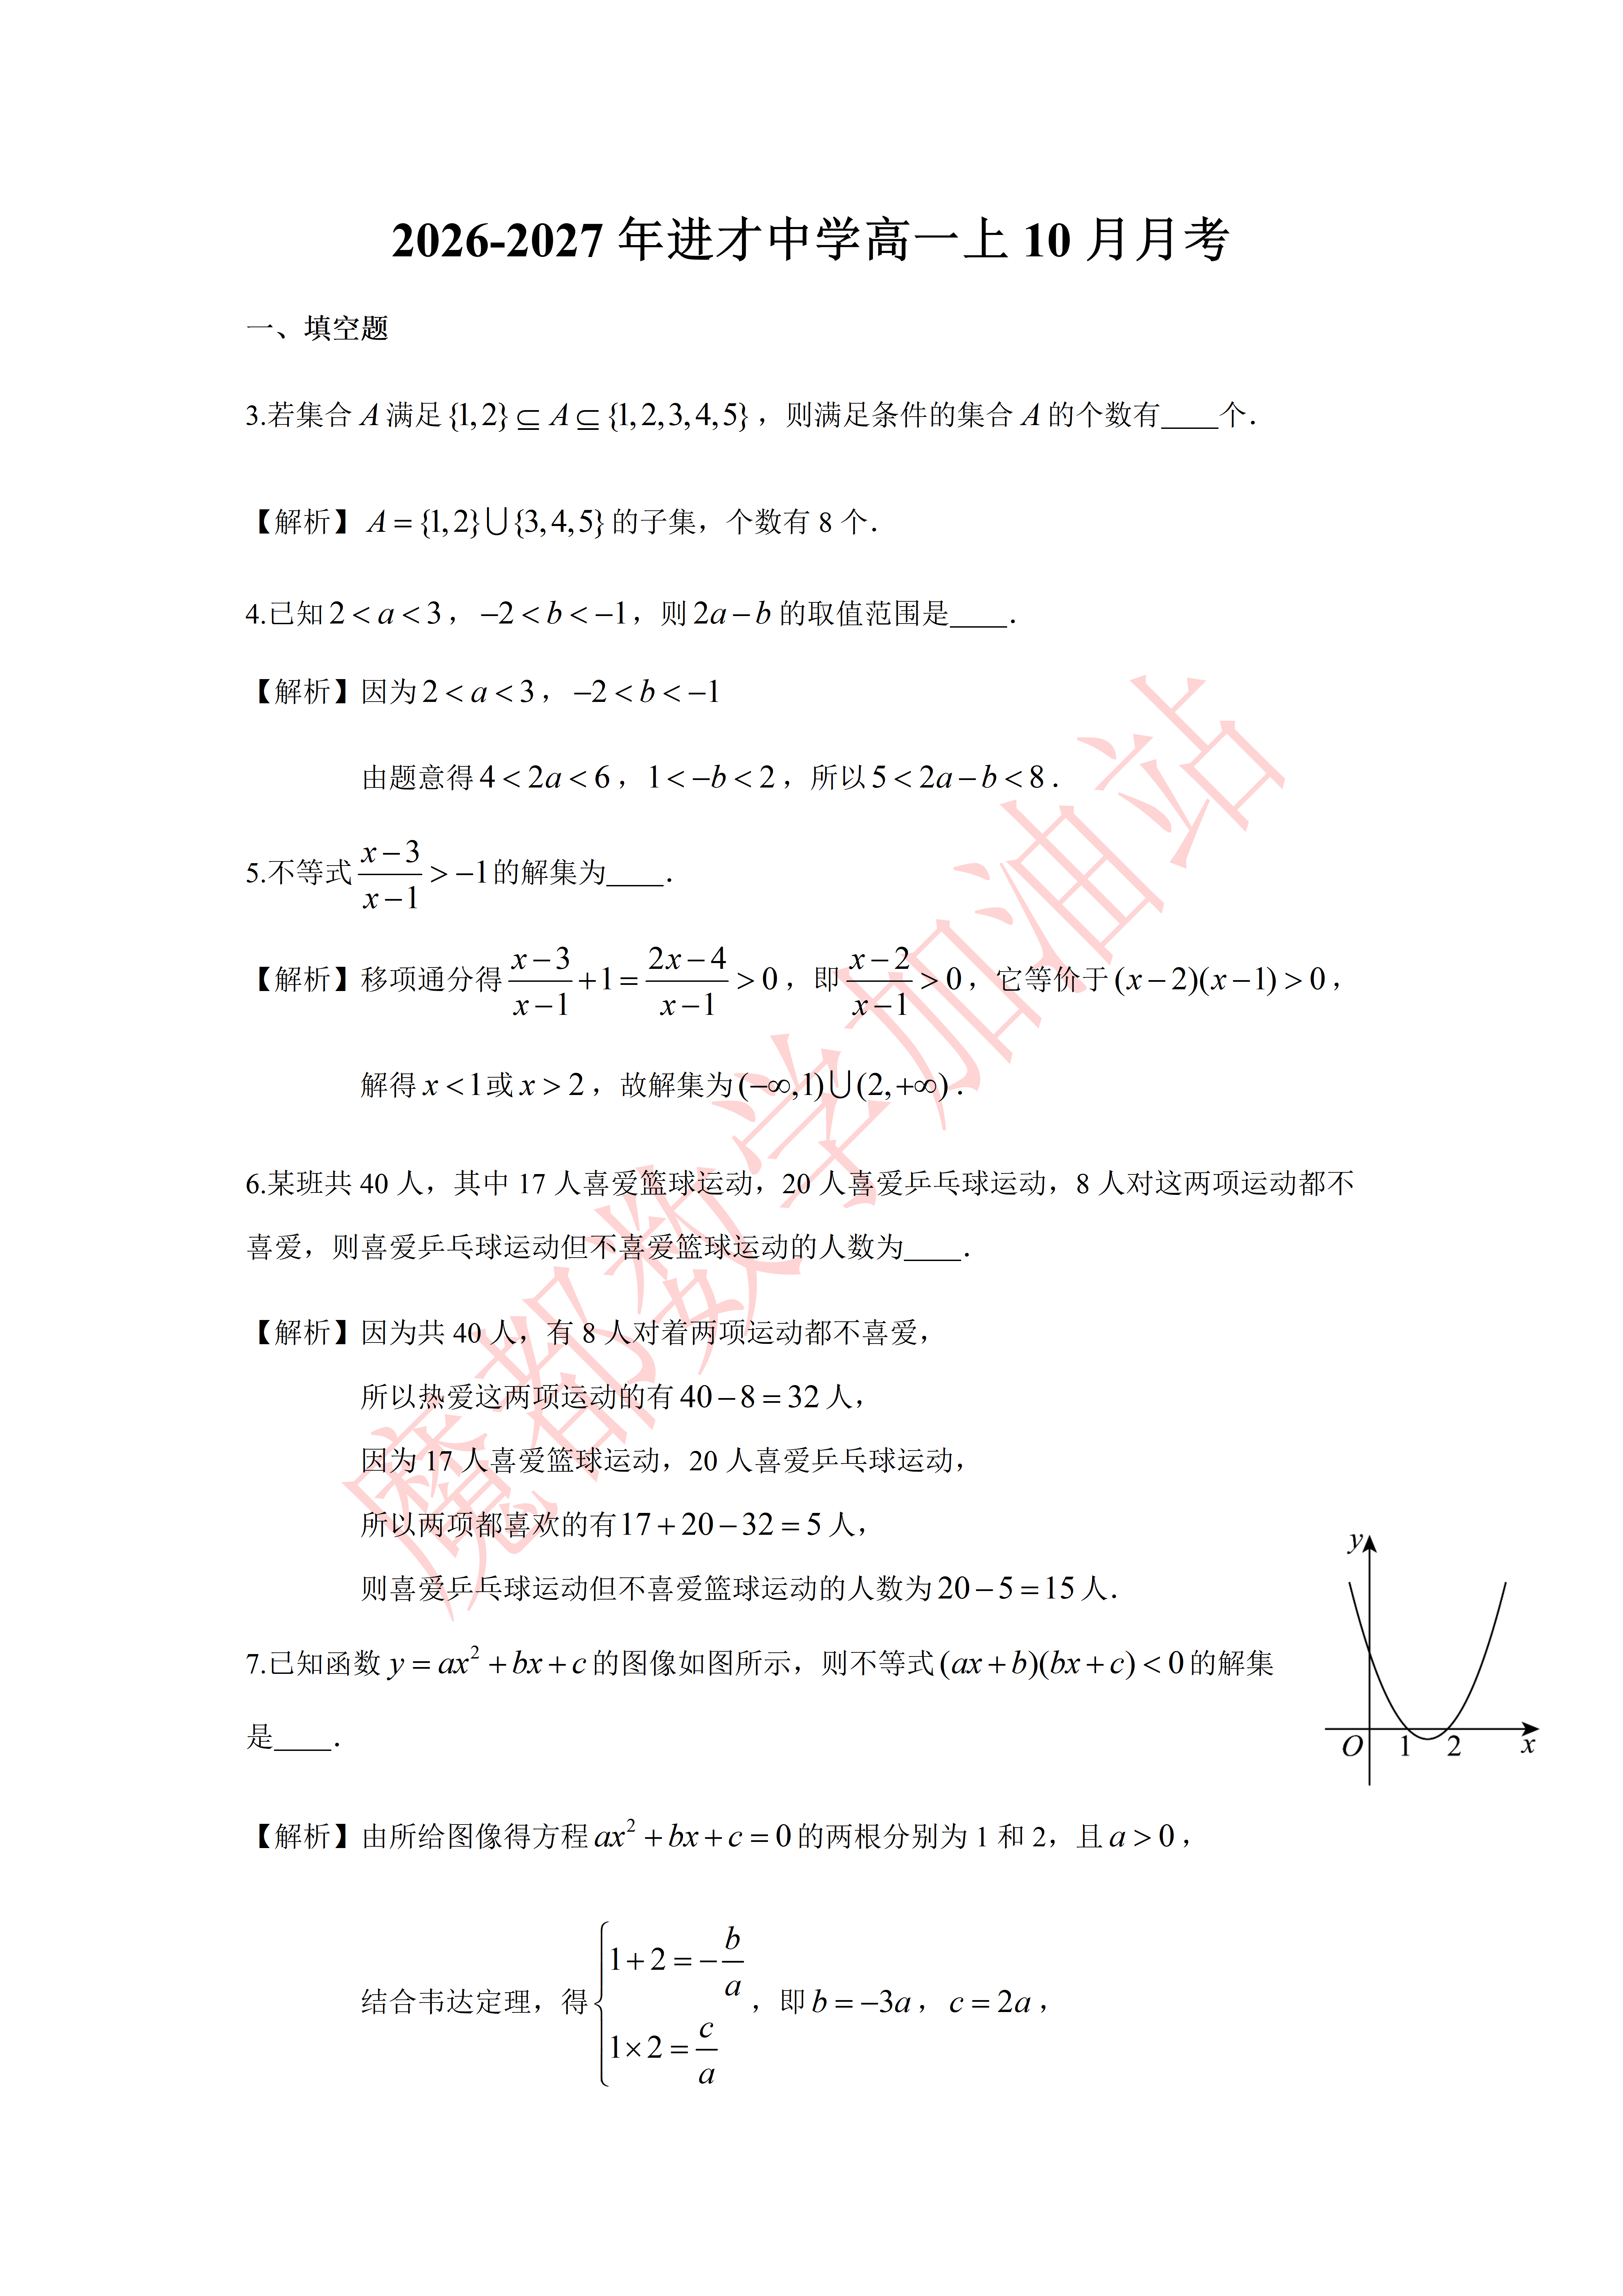
\includegraphics[width=.22\linewidth,trim=3879bp 1490bp 238bp 4492bp,clip]{../原图/高一60_进才中学_10月月考/01.png}
\end{center}

\ifanswer
\solbegin
\step{由所给图像得方程 $ax^2+bx+c=0$ 的两根分别为 1 和 2，且 $a>0$，}
\step{结合韦达定理，得 $\begin{cases}1+2=-\dfrac ba\\ 1\times2=\dfrac ca\end{cases}$，即 $b=-3a$，$c=2a$，}
\step{所以不等式 $(ax+b)(bx+c)<0$ 即 $(ax-3a)(-3ax+2a)<0$，}
\step{化简得 $(x-3)(3x-2)>0$，解得 $x<\dfrac23$ 或 $x>3$，}
\step{所以不等式 $(ax+b)(bx+c)<0$ 的解集是 $(-\infty,\dfrac23)\cup(3,+\infty)$.}
\solend
\fi

\item 已知集合 $A=\{x\mid ax=6\}$，满足 $A\subseteq\Z$，则整数 $a$ 的所有可能取值有\blankline[4.4em]个.

\ifanswer
\solbegin
\step{当 $a=0$ 时，$A=\varnothing$，而 $\varnothing\subseteq\Z$，满足题意，}
\step{当 $a\neq0$ 时，$A=\left\{\dfrac6a\right\}$，要使 $A\subseteq\Z$，则 $\dfrac6a\in\Z$，所以 $a=\pm1,\pm2,\pm3,\pm6$，}
\step{综上，整数 $a$ 的可能取值为 0，$\pm1$，$\pm2$，$\pm3$，$\pm6$，共 9 个.}
\solend
\fi

\item 设关于 $x$ 的方程 $x^2+kx+n=0$ 有两个不同实根 $x_1$、$x_2$，且 $\dfrac1{x_1}+\dfrac1{x_2}=2$，则实数 $n$ 的取值范围是\blankline[4.4em].

\ifanswer
\solbegin
\step{由于方程 $x^2+kx+n=0$ 有两个不同实根 $x_1$、$x_2$，}
\step{因此 $\Delta=k^2-4n>0$，$x_1+x_2=-k$，$x_1x_2=n$，}
\step{由 $\dfrac1{x_1}+\dfrac1{x_2}=\dfrac{x_1+x_2}{x_1x_2}=\dfrac{-k}{n}=2$，得 $k=-2n$，}
\step{因此 $\Delta=k^2-4n=4n^2-4n>0$，解得 $n<0$ 或 $n>1$，}
\step{则实数 $n$ 的取值范围是 $(-\infty,0)\cup(1,+\infty)$.}
\solend
\fi

\item 某船从甲地沿河顺流航行 $75\mathrm{km}$，到达乙码头，停留 $30\mathrm{min}$ 后再逆流航行 $126\mathrm{km}$ 到达丙地，若水流速度为 $4\mathrm{km/h}$，且该船要在 $5\mathrm{h}$ 内完成航行任务，那么船的速度至少达到\blankline[4.4em]$\mathrm{km/h}$.

\ifanswer
\solbegin
\step{设该轮船在静水中的速度是 $x$ 千米/小时，水流速度是 4 千米/小时，}
\step{由题意得 $\dfrac{75}{4+x}+0.5+\dfrac{126}{x-4}\leqslant5$，即 $9x^2-402x-552\geqslant0$，解得 $x\geqslant46$，}
\step{答：该船的速度至少是 46 千米/小时.}
\solend
\fi

\item 设实数 $a,b,c$ 满足 $a^2+b^2\leqslant c<1$，则 $a+\dfrac12b+c$ 的最小值为\blankline[4.4em].

\ifanswer
\solbegin
\step{因为 $c\geqslant a^2+b^2$，}
\step{所以 $a+\dfrac12b+c\geqslant a+\dfrac12b+a^2+b^2=\left(a+\dfrac12\right)^2+\left(b+\dfrac14\right)^2-\dfrac5{16}\geqslant-\dfrac5{16}$，}
\step{当 $a=-\dfrac12,b=-\dfrac14,c=a^2+b^2=\dfrac5{16}$（此时 $c<1$ 成立）时取到等号，}
\step{故最小值为 $-\dfrac5{16}$.}
\solend
\fi

\item 已知集合 $A=\{x\in\N^*\mid1\leqslant x\leqslant2026\}$. 设集合 $B=\{b_1,b_2,b_3,\cdots,b_n\}$ 满足 $B\subseteq A$，且对任意的 $b_i$、$b_j$、$b_k\in B(i$、$j$、$k\in\{1,2,3,\cdots,n\})$，存在 $m\in\N^*$，使得 $b_i+b_j+b_k=39m$，则 $n$ 的最大值为\blankline[4.4em].

\ifanswer
\solbegin
\step{因为 $39=1\times39=3\times13$，所以 $n$ 的最大值大于 3，}
\step{若对任意的 $b_i$、$b_j$、$b_k\in B$，存在 $m\in\N^*$，使得 $b_i+b_j+b_k=39m$，}
\step{则集合 $B$ 的元素除以 39 的余数均为 0 或均为 13 或均为 26，}
\step{即 $B=\{39,78,\cdots,39n\}$ 或 $B=\{13,52,\cdots,39n-26\}$}
\step{或 $B=\{26,65,\cdots,39n-13\}$，}
\step{若 $B=\{39,78,\cdots,39n\}$，则 $39n\leqslant2026$，}
\step{解得 $n\leqslant\dfrac{2026}{39}\in(51,52)$，此时 $n$ 的最大值为 51；}
\step{若 $B=\{13,52,\cdots,39n-26\}$，则 $39n-26\leqslant2026$，}
\step{解得 $n\leqslant\dfrac{684}{13}\in(52,53)$，此时 $n$ 的最大值为 52；}
\step{若 $B=\{26,65,\cdots,39n-13\}$，则 $39n-13\leqslant2026$，}
\step{解得 $n\leqslant\dfrac{2039}{39}\in(52,53)$，此时 $n$ 的最大值为 52；}
\step{综上，$n$ 的最大值为 52.}
\solend
\fi

\end{enumerate}

\bigsec{二、选择题}

\begin{enumerate}
\setcounter{enumi}{12}

% 第 13 题原卷无【答案】/【解析】段，答案“B”直接印在题干括号内，
% 按 高一53 第 13 题的成例括号留空、答案另提为 \ans{}（见文件头）
\item 已知 $a$、$b\in\R$，则“$|a|>|b|$”是“$a>|b|$”的\mbox{（\quad）}

\keepwithprev
A. 充分不必要条件\qquad B. 必要不充分条件

C. 充要条件\qquad D. 既不充分也不必要条件

\ifanswer
\ans{$B$}
\fi

\item 如果关于 $x$ 的一元二次方程 $x^2+2mx+(m+2)=0$ 有一正根一负根，那么 $m$ 的取值范围为\mbox{（\quad）}

\keepwithprev
A. $(-2,-1)$\qquad B. $(-1,2)$

C. $(-\infty,-1)\cup(2,+\infty)$\qquad D. $(-\infty,-2)$

\ifanswer
\solbegin
\step{设两根为 $x_1,x_2$，方程有一正根一负根，则 $\begin{cases}x_1x_2=m+2<0\\ \Delta=4m^2-4(m+2)>0\end{cases}$，}
\step{解得 $m<-2$，故选 $D$.}
\solend
\fi

\item 若不等式 $|3x-a|\leqslant x+2$ 的解集包含集合 $[0,1]$，则实数 $a$ 的取值范围为\mbox{（\quad）}

\keepwithprev
A. $[0,2]$\qquad B. $[0,1]$

C. $[1,2]$\qquad D. $(1,2)$

\ifanswer
\solbegin
% 原卷“法一：”“法二：”排红色加粗（全卷唯一红字），本稿按全稿子题标号样式排 \stepm
% （详见文件头“与原卷的排版差异”⑦）
\stepm{法一：}{不等式 $|3x-a|\leqslant x+2$ 化为 $2x-2\leqslant a\leqslant4x+2$，}
% 原卷此句缺动词（疑漏“对”字），照录未改（见文件头“原卷存疑”④）
\step{$[0,1]$ 使 $2x-2\leqslant a\leqslant4x+2$ 成立，则 $0\leqslant a\leqslant2$，故选 $A$.}
\stepm{法二：}{将两边平方整理得 $8x^2-(6a+4)x+a^2-4\leqslant0$ 对 $[0,1]$ 恒成立，}
\step{则有 $\begin{cases}a^2-4\leqslant0\\ a^2-6a\leqslant0\end{cases}$，解得 $0\leqslant a\leqslant2$，故选 $A$.}
\solend
\fi

\item 数学组 Y 老师在白纸上写下以下四个命题：

①这四个命题中至少有一个是真的；②这四个命题中至少有两个是真的；

③这四个命题中至少有两个是假的；④这四个命题中至少有一个是假的；

每个命题非真即假. 问 Y 老师在纸上写的假命题有几个？\mbox{（\quad）}

\keepwithprev
A. 0\qquad B. 1

C. 2\qquad D. 3

\ifanswer
\solbegin
\step{设四个命题中真命题的个数为 $t$，则①真 $\iff t\geqslant1$，②真 $\iff t\geqslant2$，}
\step{③真 $\iff t\leqslant2$，④真 $\iff t\leqslant3$.}
\step{逐一检验：$t=0$ 时③④为真，应为 $t=2$，矛盾；}
\step{$t=1$ 时①③④为真，应为 $t=3$，矛盾；}
\step{$t=2$ 时四个命题全为真，应为 $t=4$，矛盾；}
\step{$t=3$ 时①②④为真、③为假，恰有 3 个真命题，符合；}
\step{$t=4$ 时①②为真，应为 $t=2$，矛盾.}
\step{所以恰有 1 个假命题，故选 $B$.}
\solend
\fi

\end{enumerate}

\bigsec{三、解答题}

\begin{enumerate}
\setcounter{enumi}{16}

\item 已知：$x\in\R$，$a=x^2-1$，$b=4x+5$. 求证：$a$、$b$ 中至少有一个大于等于 0.

\ifanswer
\solbegin
\step{假设 $a$、$b$ 都小于 0，即 $a<0$，$b<0$，则 $a+b<0$.}
\step{又 $a+b=x^2-1+4x+5=x^2+4x+4=(x+2)^2\geqslant0$，}
\step{这与假设所得 $a+b<0$ 矛盾，故假设不成立，}
\step{所以 $a$、$b$ 中至少有一个大于等于 0.}
\solend
\fi

\ansspace[6]

% 原卷 A、B 两个集合定义之间排半角逗号“,”（5 倍放大核，右侧字距 19px，与全卷全角“，”的 65—79px 字距判然有别）；
% 本稿原误抄为全角“，”——已照录原卷半角（见文件头“与原卷的排版差异”⑤）
\item 已知集合 $A=\{x\mid4\leqslant x\leqslant12\}$,$B=\{x\mid a\leqslant x\leqslant2a+1\}$.

（1）若 $a=2$，求 $\overline A\cap B$；

（2）已知 $A\cup B=A$，求实数 $a$ 的取值范围.

\ifanswer
\solbegin
\stepm{(1)}{当 $a=2$ 时，$B=\{x\mid2\leqslant x\leqslant5\}$，}
\step{而 $A=\{x\mid4\leqslant x\leqslant12\}$，则 $\overline A=(-\infty,4)\cup(12,+\infty)$，所以 $\overline A\cap B=[2,4)$.}
\stepm{(2)}{$A\cup B=A$ 即 $B\subseteq A$.}
\stepm{①}{当 $B=\varnothing$ 时，$a>2a+1$，即 $a<-1$，符合；}
\stepm{②}{当 $B\neq\varnothing$ 时，需 $a\leqslant2a+1$ 且 $a\geqslant4$ 且 $2a+1\leqslant12$，即 $4\leqslant a\leqslant\dfrac{11}2$.}
\step{综上，$a$ 的取值范围是 $(-\infty,-1)\cup\left[4,\dfrac{11}2\right]$.}
\solend
\fi

\ansspace[8]

\item （1）若关于 $x$ 的不等式 $ax^2-3x+2<0$ 的解集不是空集，求实数 $a$ 的取值范围；

（2）求关于 $x$ 的不等式 $ax^2-3x+2>ax-1$ 的解集.

\ifanswer
\solbegin
\stepm{(1)}{若 $a>0$，关于 $x$ 的不等式 $ax^2-3x+2<0$ 的解集不空，}
\step{所以一元二次方程 $ax^2-3x+2=0$ 的判别式大于零，}
\step{即 $(-3)^2-8a>0\Rightarrow a<\dfrac98$，结合 $a>0$ 得 $0<a<\dfrac98$；}
\step{若 $a\leqslant0$，则关于 $x$ 的不等式 $ax^2-3x+2<0$ 的解集不是空集；}
\step{综上，实数 $a$ 的取值范围是 $\left(-\infty,\dfrac98\right)$.}
\stepm{(2)}{$ax^2-3x+2>ax-1\Rightarrow ax^2-(a+3)x+3>0\Rightarrow(ax-3)(x-1)>0$，}
\step{当 $a=0$ 时，不等式为 $x-1<0$，不等式的解集为 $\{x\mid x<1\}$；}
\step{当 $a<0$ 时，不等式化为 $\left(x-\dfrac3a\right)(x-1)<0$，}
\step{不等式的解集为 $\left\{x\mid\dfrac3a<x<1\right\}$，}
\step{当 $a>0$ 时，方程 $ax^2-3x+2=ax-1$ 的两个根分别为：$\dfrac3a,1$.}
\step{当 $a=3$ 时，两根相等，故不等式的解集为 $\{x\mid x\neq1\}$；}
\step{当 $a>3$ 时，$\dfrac3a<1$，不等式的解集为 $\left\{x\mid x<\dfrac3a\right.$ 或 $\left.x>1\right\}$；}
\step{当 $0<a<3$ 时，$\dfrac3a>1$，不等式的解集为 $\left\{x\mid x<1\right.$ 或 $\left.x>\dfrac3a\right\}$；}
\step{综上所述，当 $a<0$ 时，不等式的解集为 $\left\{x\mid\dfrac3a<x<1\right\}$，}
\step{当 $a=0$ 时，不等式的解集为 $\{x\mid x<1\}$，}
\step{当 $0<a<3$ 时，不等式的解集为 $\left\{x\mid x<1\right.$ 或 $\left.x>\dfrac3a\right\}$，}
\step{当 $a=3$ 时，不等式的解集为 $\{x\mid x\neq1\}$，}
\step{当 $a>3$ 时，不等式的解集为 $\left\{x\mid x<\dfrac3a\right.$ 或 $\left.x>1\right\}$.}
\solend
\fi

\ansspace[8]

\item 设命题 $p$：对任意 $x\in\R$，使得不等式 $mx^2-mx+2>0$ 恒成立；命题 $q$：存在 $0\leqslant x\leqslant3$，不等式 $2x-2\geqslant|m|$ 成立.

（1）若 $p$ 为真命题，求实数 $m$ 的取值范围；

（2）若 $p$、$q$ 有且只有一个是真命题，求实数 $m$ 的取值范围.

\ifanswer
\solbegin
\stepm{(1)}{因为 $p:\forall x\in\R$，$mx^2-mx+2>0$ 为真命题，}
\step{所以当 $m=0$ 时，不等式为 $2>0$，在 $\R$ 上恒成立，符合题意；}
\step{当 $m\neq0$ 时，$\begin{cases}m>0\\ \Delta=m^2-8m<0\end{cases}$，解得 $0<m<8$.}
\step{综上，实数 $m$ 的取值范围为 $[0,8)$.}
\stepm{(2)}{若 $q$ 为真命题，即 $q:\exists0\leqslant x\leqslant3$，$2x-2\geqslant|m|$，}
\step{则对于 $0\leqslant x\leqslant3$，$(2x-2)_{max}\geqslant|m|$.}
\step{由于 $0\leqslant x\leqslant3$，$2x-2\in[-2,4]$，所以 $|m|\leqslant4$，解得 $-4\leqslant m\leqslant4$，}
\step{又因为 $p$、$q$ 有且只有一个是真命题，}
\step{所以当 $p$ 真 $q$ 假时，$\begin{cases}0\leqslant m<8\\ m<-4\text{或}m>4\end{cases}$，解得 $4<m<8$；}
\step{当 $p$ 假 $q$ 真时，$\begin{cases}m<0\text{或}m\geqslant8\\ -4\leqslant m\leqslant4\end{cases}$，解得 $-4\leqslant m<0$；}
\step{综上，实数 $m$ 的取值范围为 $[-4,0)\cup(4,8)$.}
\solend
\fi

\ansspace[10]

\item 已知集合 $A=\{a_1,a_2,\cdots,a_k\}(k\geqslant2)$. 其中 $a_i\in\N^*(i=1,2,\cdots,k)$. 若对于任意的 $a\in A$，总有 $\dfrac1a\notin A$，则称集合 $A$ 具有性质 $P$. 由 $A$ 中的元素构成两个相应的集合：$S=\{(a,b)\mid a\in A,b\in A,ab\in A\}$，$T=\left\{(a,b)\mid a\in A,b\in A,\dfrac ab\in A\right\}$，其中 $(a,b)$ 是有序数对，集合 $S$ 和 $T$ 中的元素个数分别为 $m$ 和 $n$.

（1）检验集合 $\{2,3,6\}$ 与 $\{1,2,4\}$ 是否具有性质 $P$，并对其中具有性质 $P$ 的集合，写出相应的集合 $S$ 和 $T$；

（2）对任何具有性质 $P$ 的集合 $A$，$n$ 的最大值为多少？（直接写出答案，无需说明理由）；

% 原卷题干的小问编号跳号：印作 (1)(2)(4)，本稿照录 (4)、未改成 (3)（见文件头“原卷存疑”①）
（4）判断 $m$ 和 $n$ 的大小关系，并证明你的结论.

\ifanswer
\solbegin
\stepm{(1)}{因为 $\dfrac12\in\{1,2,4\}$，所以 $\{1,2,4\}$ 不具有性质 $P$；}
\step{因为 $\dfrac12\notin\{2,3,6\}$，$\dfrac13\notin\{2,3,6\}$，$\dfrac16\notin\{2,3,6\}$，所以 $\{2,3,6\}$ 具有性质 $P$.}
\step{$S=\{(2,3),(3,2)\}$，$T=\{(6,2),(6,3)\}$；}
\stepm{(2)}{因为对于任意的 $a\in A$，总有 $\dfrac1a\notin A$，所以 $1\notin A$，}
% 原卷此处印作“$\{(a_i,a_i)\}\in T$”，与上一句“$1\notin A$”及下文“最多为 $C_k^2$”的推理
% 均不自洽（应为“$\notin$”），已 8 倍放大确认无斜线；照录未改（见文件头“原卷存疑”③）
\step{从而 $\{(a_i,a_i)\}\in T(i=1,2,\cdots,k)$.}
\step{因为 $a\in A,b\in A,\dfrac ab\in A$，所以当 $i\neq j$ 时，}
\step{$(a_i,a_j)\in T$ 和 $(a_j,a_i)\in T(i,j=1,2,\cdots,k)$ 至多有一个成立，}
\step{所以集合 $T$ 中的元素个数最多为 $C_k^2=\dfrac{k(k-1)}2$，即 $n\leqslant\dfrac{k(k-1)}2$.}
% 原卷【解析】把第 (4) 问标作“(3)”（与题干跳号相应），本稿照录未改（见文件头“原卷存疑”①）
\stepm{(3)}{$m=n$，证明如下：}
\step{①设 $(a,b)\in T$，则 $a\in A,b\in A,\dfrac ab\in A$. 设 $c=\dfrac ab$，则 $a=bc$，}
\step{故 $b\in A$，$c\in A$，$bc\in A$，从而 $(b,c)\in S$，}
\step{即对 $\forall(a,b)\in T$，总 $\exists c$ 使 $(b,c)\in S$，从而 $n\leqslant m$.}
\step{②设 $(p,q)\in S$，则 $p\in A$，$q\in A$，$pq\in A$.}
\step{设 $r=pq$，则 $q=\dfrac rp$，故 $r\in A,p\in A,\dfrac rp\in A$，从而 $(r,p)\in T$，}
\step{即对 $\forall(p,q)\in S$，总 $\exists r$ 使 $(r,p)\in T$，从而 $m\leqslant n$.}
\step{由①②得 $m=n$.}
\solend
\fi

\ansspace*[10]

\end{enumerate}

\end{document}
"
% 紧凑版：xelatex "\def\iscompact{1}% 高一60_进才中学_10月月考.tex
%   —— 高一上数学“2026-2027 年进才中学高一上 10 月月考”（讲评版）
% 试卷版：xelatex 高一60_进才中学_10月月考.tex
% 答案版：xelatex "\def\isanswer{1}% 高一60_进才中学_10月月考.tex
%   —— 高一上数学“2026-2027 年进才中学高一上 10 月月考”（讲评版）
% 试卷版：xelatex 高一60_进才中学_10月月考.tex
% 答案版：xelatex "\def\isanswer{1}\input{高一60_进才中学_10月月考.tex}"
% 紧凑版：xelatex "\def\iscompact{1}\input{高一60_进才中学_10月月考.tex}"
%
% 原文链接：https://mp.weixin.qq.com/s/2ZLKB3IONEDhcUAfAAYE2A。
% 公众号“魔都数学加油站”作者破晓于 2026-10-14 22:15 发布。
% 原图 9 张（`原图/高一60_进才中学_10月月考/01..09.png`）：第 1—8 页 4762×6735，
% 第 9 页 2560×3620（同一篇内两档分辨率）。
%
% 卷首标题：照卷面印作“2026--2027 年进才中学高一上 10 月月考”（公众号标题中的“上海市”
% 卷面标题行没有，本稿照卷面），年份区间按全稿惯例排 en dash。原卷只有一行标题、无副标题。
%
% 篇幅与题号：原卷自第 3 题起编号（第 1、2 题不在本卷内）。填空题 3—12（10 题）、
% 选择题 13—16（4 题）、解答题 17—21（5 题），共 19 题。本稿沿用原节与原题号，
% 只改排为全稿统一的大节样式（原卷小节标题为“一、填空题”“二、选择题”“三、解答题”）。
%
% 讲评版：原卷每题下直接印【答案】或【解析】。**只印【解析】的 18 题**，本稿按全稿口径
% 收进答案版、不另提 \ans{}——第 14、15、16 题的结论写在解析末句（“故选 D／A／B”），
% 亦照录在解析内。**第 13 题原卷没有任何【答案】/【解析】段**，答案“B”直接印在题干括号内
% （“（ B ）”），本稿按 高一53 第 13 题的成例把括号留空、答案另提为 \ans{$B$}（见下）。
%
% 副标题：原卷未印副标题。本稿按“知识模块”口径标作“集合与常用逻辑用语、不等式”：
% 19 题中集合与常用逻辑用语 10 题（第 3、6、8、12、13、16、17、18、20、21 题，
% 含子集计数、韦恩图容斥、集合运算、命题与充要条件、反证法、新定义），
% 不等式 9 题（含不等式性质、分式不等式、二次函数与解集、韦达定理与判别式、
% 不等式应用、最值、根的分布、绝对值不等式恒成立、含参二次不等式：第 4、5、7、9、10、
% 11、14、15、19 题），两类均远超三分之一，故并标。口径同 高一46、高一47、高一48、
% 高一51—高一59。
%
% 与原卷的排版差异：
%   ① 原卷每题下直接印【答案】/【解析】，本稿按全稿惯例将答案与解析置于答案版，试卷版保持干净；
%   ② 原卷未印副标题，本稿按“知识模块”口径补出；
%   ③ 原卷填空横线约两个字宽，本稿按全稿惯例统一排 \blankline[4.4em]；
%   ④ 原卷实数集排斜体 $R$（第 13、17、20 题）、正整数集排 $N^*$（第 12、21 题）、
%      整数集排粗体 $\mathbf{Z}$（第 8 题），本稿按全稿惯例改用 $\R$、$\N^*$、$\Z$；
%      空集记号统一为 \varnothing；
%   ⑤ 原卷在数学式内多处用半角逗号（如 $x_1,x_2$、$a,b\in R$，以及第 18 题题干
%      $A=\{x\mid4\leqslant x\leqslant12\}$,$B=\{x\mid a\leqslant x\leqslant2a+1\}$ 之间的逗号），
%      均照录未强改（第 18 题题干那一处本稿首轮曾误作全角“，”，第二轮已订正）；
%      句末句点按全稿惯例排西文句点；
%   ⑥ 第 13 题印在题干括号内的答案“B”移入 \ans{}，见上；
%   ⑦ 第 15 题【解析】的“法一：”“法二：”标号原卷排**红色加粗**（全卷唯一的红字，2 处），
%      本稿按全稿子题标号样式排 \stepm{法一：}{…}、\stepm{法二：}{…}（加粗着色、不改黑色
%      基调），冒号照原卷排全角；
%   ⑧ 第 7 题的图像原卷排在题干右侧（与题干第 1 行同高），本稿居中排在题干之后；
%      图自原图第 01 页裁切（trim），不另存图片文件；
%   ⑨ 原卷第 10 题的长度与速度单位原卷排斜体（$75km$、$4km/h$ 等），本稿按全稿惯例
%      改排正体 $\mathrm{km}$、$\mathrm{km/h}$（同 高一56 第 13 题）；每道解答题原卷未留
%      作答空白，本稿按全稿惯例加 \ansspace。
%
% 原卷存疑（照录未改，见源码中该处上方注释）：
%   ① 第 21 题题干的小问编号**跳号**：印作 (1)(2)(4)，而紧随其后的【解析】按 (1)(2)(3) 写
%      —— 题干第 (4) 问实为第 (3) 问。本稿题干照录 (1)(2)(4)、解析照录 (3)，未改
%      （与 高一22 第 16 题“解析误标 (2)”同一处理）。
%   ② 第 6 题【解析】“有 8 人**对着**两项运动都不喜爱”，“对着”疑为“对这”之误，照录未改。
%   ③ 第 21(2) 题【解析】首行“所以 $1\notin A$，从而 $\{(a_i,a_i)\}\in T(i=1,2,\cdots,k)$”
%      —— 由 $1\notin A$ 应得 $(a_i,a_i)\notin T$（因 $a_i/a_i=1$），与紧随的“$T$ 中元素
%      个数最多为 $C_k^2$”这一推理亦只有“$\notin$”才自洽；原卷此处印作“$\in$”，
%      已 8 倍放大确认无斜线。**照录原卷的 $\in$、未改**。
%   ④ 第 15 题【解析】法一“$[0,1]$ 使 $2x-2\leqslant a\leqslant4x+2$ 成立”一句缺动词
%      （疑漏“对”字），照录未改。
%
\documentclass[a4paper,11pt]{article}
\usepackage{common}

\begin{document}

\examtitlest[3]{2026--2027 年进才中学高一上 10 月月考}{集合与常用逻辑用语、不等式}

\bigsec{一、填空题}

\begin{enumerate}
\setcounter{enumi}{2}

\item 若集合 $A$ 满足 $\{1,2\}\subseteq A\subseteq\{1,2,3,4,5\}$，则满足条件的集合 $A$ 的个数有\blankline[4.4em]个.

\ifanswer
\solbegin
\step{$A=\{1,2\}\cup\{3,4,5\}$ 的子集，个数有 8 个.}
\solend
\fi

\item 已知 $2<a<3$，$-2<b<-1$，则 $2a-b$ 的取值范围是\blankline[4.4em].

\ifanswer
\solbegin
\step{因为 $2<a<3$，$-2<b<-1$，}
\step{由题意得 $4<2a<6$，$1<-b<2$，所以 $5<2a-b<8$.}
\solend
\fi

\item 不等式 $\dfrac{x-3}{x-1}>-1$ 的解集为\blankline[4.4em].

\ifanswer
\solbegin
\step{移项通分得 $\dfrac{x-3}{x-1}+1=\dfrac{2x-4}{x-1}>0$，即 $\dfrac{x-2}{x-1}>0$，它等价于 $(x-2)(x-1)>0$，}
\step{解得 $x<1$ 或 $x>2$，故解集为 $(-\infty,1)\cup(2,+\infty)$.}
\solend
\fi

\item 某班共 40 人，其中 17 人喜爱篮球运动，20 人喜爱乒乓球运动，8 人对这两项运动都不喜爱，则喜爱乒乓球运动但不喜爱篮球运动的人数为\blankline[4.4em].

\ifanswer
\solbegin
% 原卷作“对着两项运动都不喜爱”（疑为“对这”之误），照录未改（见文件头“原卷存疑”②）
\step{因为共 40 人，有 8 人对着两项运动都不喜爱，}
\step{所以热爱这两项运动的有 $40-8=32$ 人，}
\step{因为 17 人喜爱篮球运动，20 人喜爱乒乓球运动，}
\step{所以两项都喜欢的有 $17+20-32=5$ 人，}
\step{则喜爱乒乓球运动但不喜爱篮球运动的人数为 $20-5=15$ 人.}
\solend
\fi

\item 已知函数 $y=ax^2+bx+c$ 的图像如图所示，则不等式 $(ax+b)(bx+c)<0$ 的解集是\blankline[4.4em].

% 原图第 01 页题干右侧的图像直接裁取。裁框取图外框 x 3887–4516、y 4500–5237
% （四周各留约 8px），trim=左 3879bp／下 1490bp／右 238bp／上 4492bp
% （页宽 4762、页高 6735）。
\begin{center}
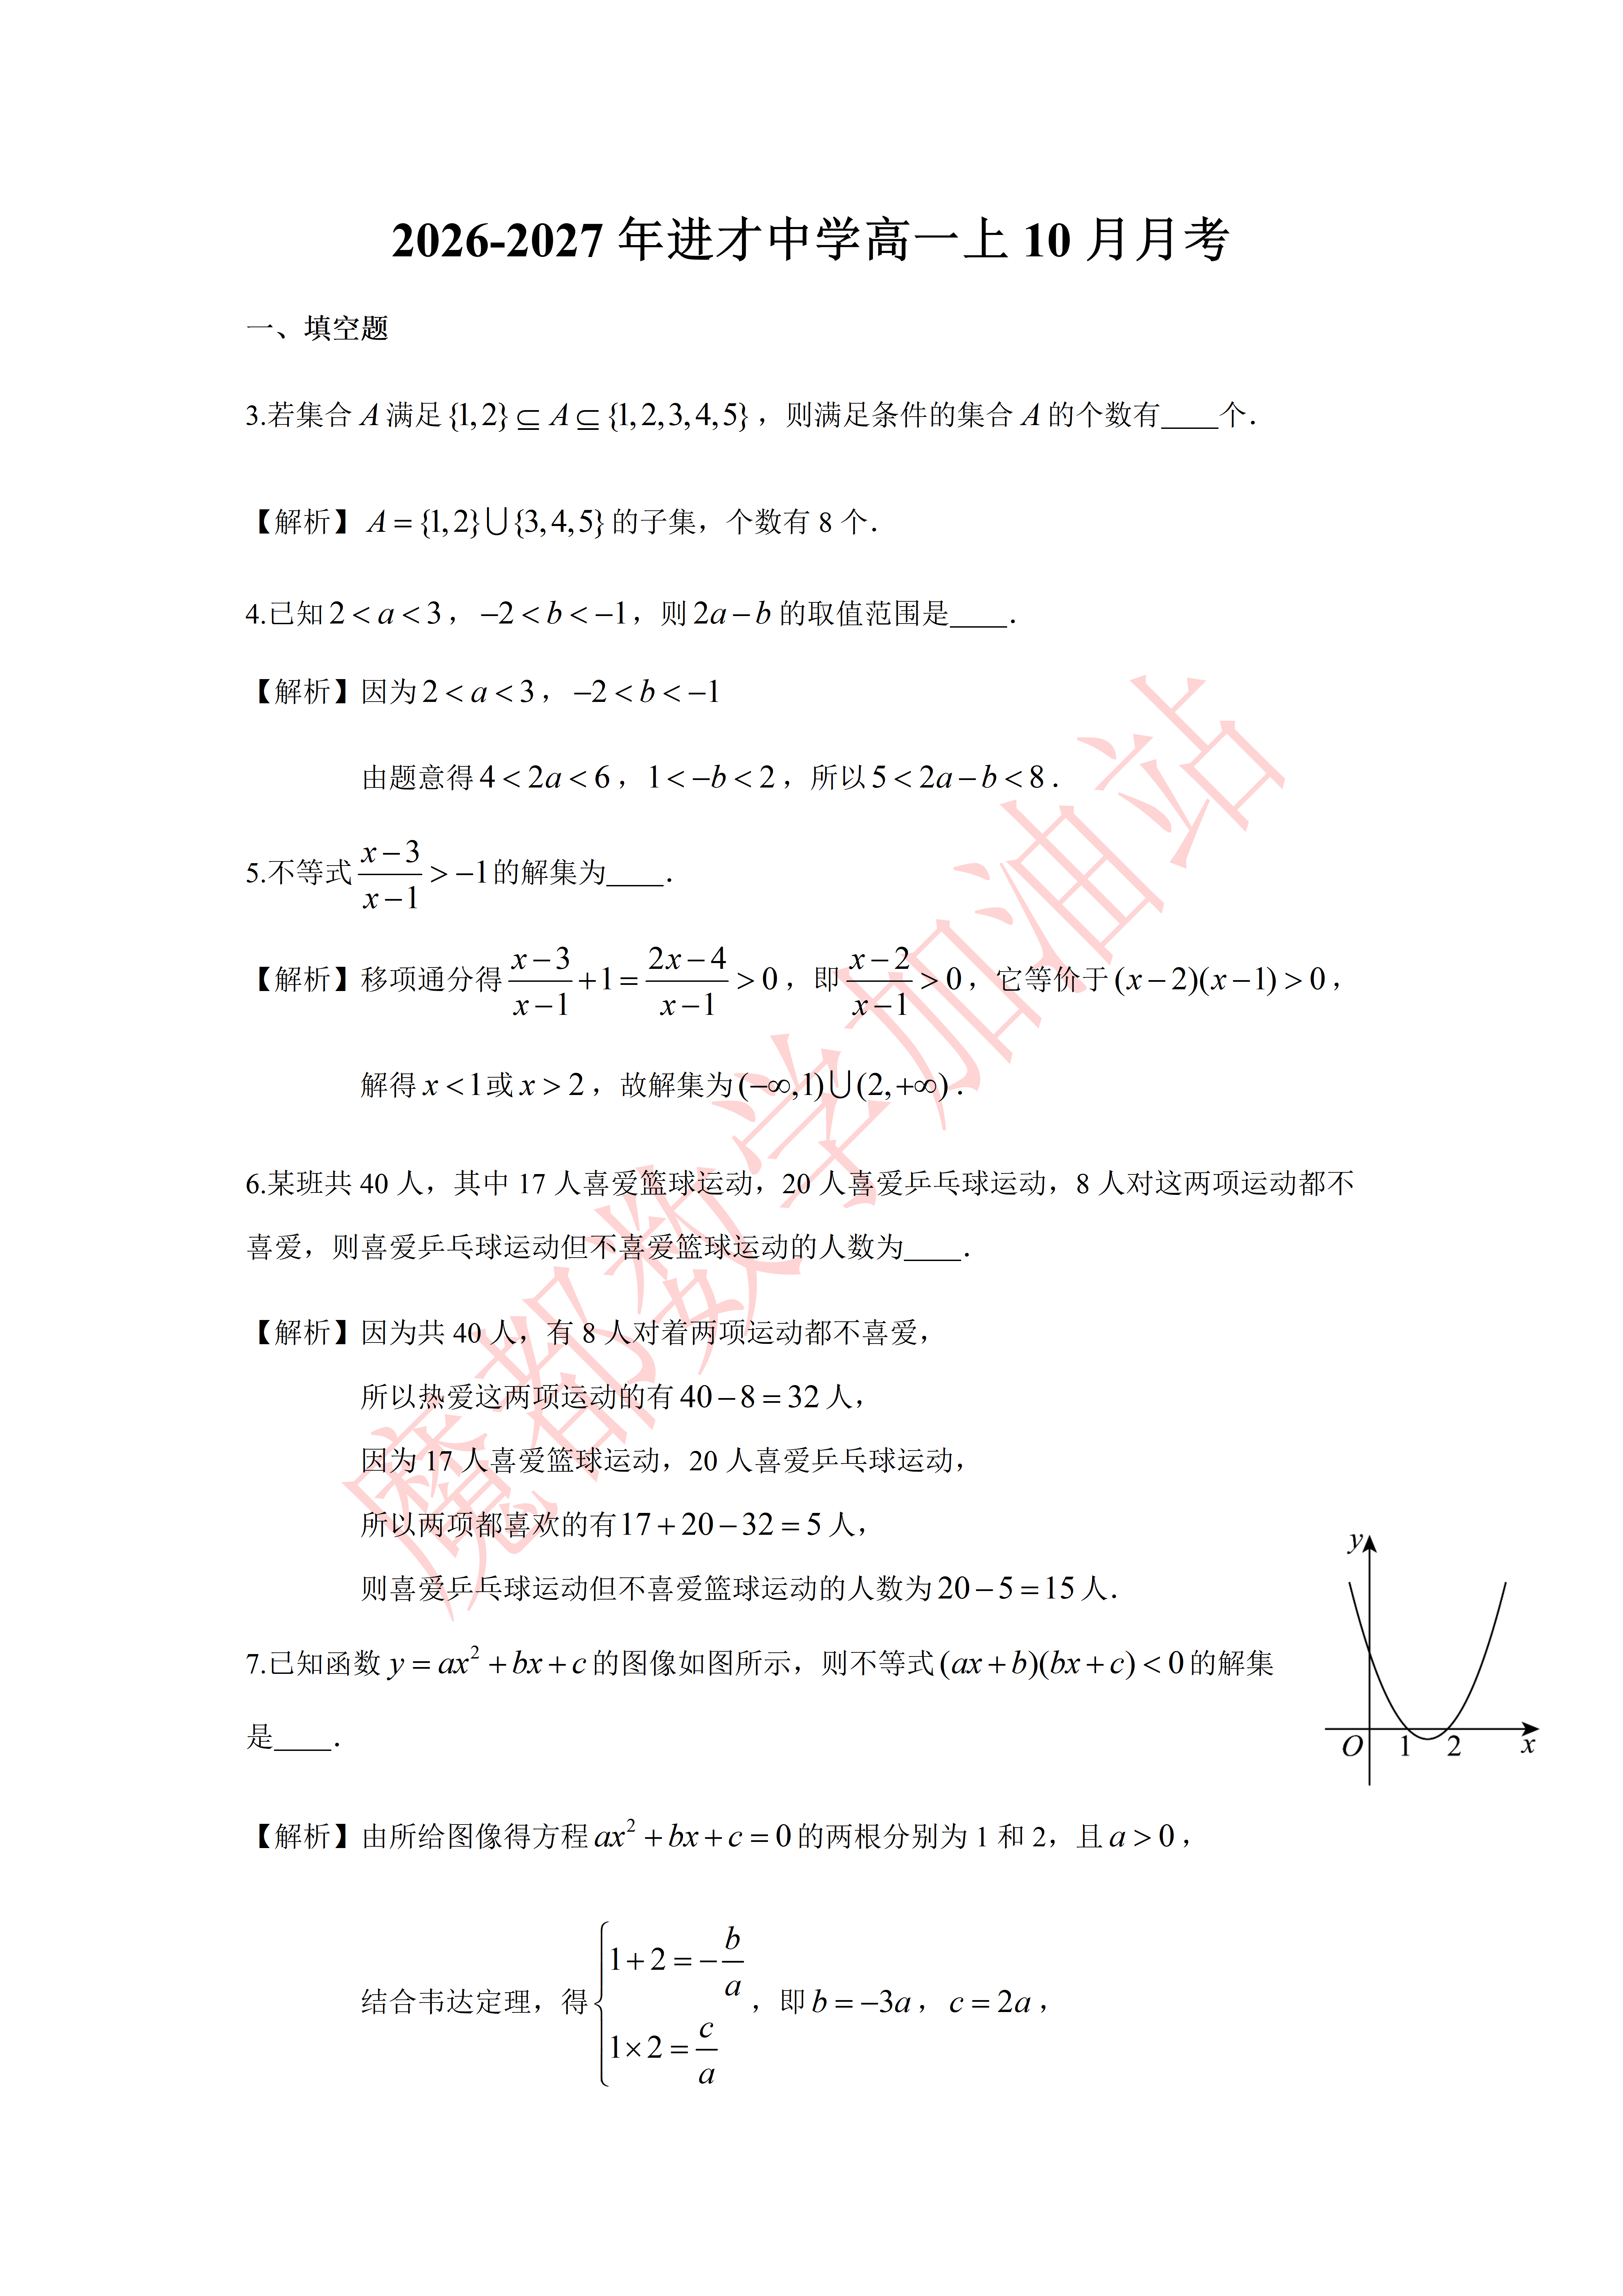
\includegraphics[width=.22\linewidth,trim=3879bp 1490bp 238bp 4492bp,clip]{../原图/高一60_进才中学_10月月考/01.png}
\end{center}

\ifanswer
\solbegin
\step{由所给图像得方程 $ax^2+bx+c=0$ 的两根分别为 1 和 2，且 $a>0$，}
\step{结合韦达定理，得 $\begin{cases}1+2=-\dfrac ba\\ 1\times2=\dfrac ca\end{cases}$，即 $b=-3a$，$c=2a$，}
\step{所以不等式 $(ax+b)(bx+c)<0$ 即 $(ax-3a)(-3ax+2a)<0$，}
\step{化简得 $(x-3)(3x-2)>0$，解得 $x<\dfrac23$ 或 $x>3$，}
\step{所以不等式 $(ax+b)(bx+c)<0$ 的解集是 $(-\infty,\dfrac23)\cup(3,+\infty)$.}
\solend
\fi

\item 已知集合 $A=\{x\mid ax=6\}$，满足 $A\subseteq\Z$，则整数 $a$ 的所有可能取值有\blankline[4.4em]个.

\ifanswer
\solbegin
\step{当 $a=0$ 时，$A=\varnothing$，而 $\varnothing\subseteq\Z$，满足题意，}
\step{当 $a\neq0$ 时，$A=\left\{\dfrac6a\right\}$，要使 $A\subseteq\Z$，则 $\dfrac6a\in\Z$，所以 $a=\pm1,\pm2,\pm3,\pm6$，}
\step{综上，整数 $a$ 的可能取值为 0，$\pm1$，$\pm2$，$\pm3$，$\pm6$，共 9 个.}
\solend
\fi

\item 设关于 $x$ 的方程 $x^2+kx+n=0$ 有两个不同实根 $x_1$、$x_2$，且 $\dfrac1{x_1}+\dfrac1{x_2}=2$，则实数 $n$ 的取值范围是\blankline[4.4em].

\ifanswer
\solbegin
\step{由于方程 $x^2+kx+n=0$ 有两个不同实根 $x_1$、$x_2$，}
\step{因此 $\Delta=k^2-4n>0$，$x_1+x_2=-k$，$x_1x_2=n$，}
\step{由 $\dfrac1{x_1}+\dfrac1{x_2}=\dfrac{x_1+x_2}{x_1x_2}=\dfrac{-k}{n}=2$，得 $k=-2n$，}
\step{因此 $\Delta=k^2-4n=4n^2-4n>0$，解得 $n<0$ 或 $n>1$，}
\step{则实数 $n$ 的取值范围是 $(-\infty,0)\cup(1,+\infty)$.}
\solend
\fi

\item 某船从甲地沿河顺流航行 $75\mathrm{km}$，到达乙码头，停留 $30\mathrm{min}$ 后再逆流航行 $126\mathrm{km}$ 到达丙地，若水流速度为 $4\mathrm{km/h}$，且该船要在 $5\mathrm{h}$ 内完成航行任务，那么船的速度至少达到\blankline[4.4em]$\mathrm{km/h}$.

\ifanswer
\solbegin
\step{设该轮船在静水中的速度是 $x$ 千米/小时，水流速度是 4 千米/小时，}
\step{由题意得 $\dfrac{75}{4+x}+0.5+\dfrac{126}{x-4}\leqslant5$，即 $9x^2-402x-552\geqslant0$，解得 $x\geqslant46$，}
\step{答：该船的速度至少是 46 千米/小时.}
\solend
\fi

\item 设实数 $a,b,c$ 满足 $a^2+b^2\leqslant c<1$，则 $a+\dfrac12b+c$ 的最小值为\blankline[4.4em].

\ifanswer
\solbegin
\step{因为 $c\geqslant a^2+b^2$，}
\step{所以 $a+\dfrac12b+c\geqslant a+\dfrac12b+a^2+b^2=\left(a+\dfrac12\right)^2+\left(b+\dfrac14\right)^2-\dfrac5{16}\geqslant-\dfrac5{16}$，}
\step{当 $a=-\dfrac12,b=-\dfrac14,c=a^2+b^2=\dfrac5{16}$（此时 $c<1$ 成立）时取到等号，}
\step{故最小值为 $-\dfrac5{16}$.}
\solend
\fi

\item 已知集合 $A=\{x\in\N^*\mid1\leqslant x\leqslant2026\}$. 设集合 $B=\{b_1,b_2,b_3,\cdots,b_n\}$ 满足 $B\subseteq A$，且对任意的 $b_i$、$b_j$、$b_k\in B(i$、$j$、$k\in\{1,2,3,\cdots,n\})$，存在 $m\in\N^*$，使得 $b_i+b_j+b_k=39m$，则 $n$ 的最大值为\blankline[4.4em].

\ifanswer
\solbegin
\step{因为 $39=1\times39=3\times13$，所以 $n$ 的最大值大于 3，}
\step{若对任意的 $b_i$、$b_j$、$b_k\in B$，存在 $m\in\N^*$，使得 $b_i+b_j+b_k=39m$，}
\step{则集合 $B$ 的元素除以 39 的余数均为 0 或均为 13 或均为 26，}
\step{即 $B=\{39,78,\cdots,39n\}$ 或 $B=\{13,52,\cdots,39n-26\}$}
\step{或 $B=\{26,65,\cdots,39n-13\}$，}
\step{若 $B=\{39,78,\cdots,39n\}$，则 $39n\leqslant2026$，}
\step{解得 $n\leqslant\dfrac{2026}{39}\in(51,52)$，此时 $n$ 的最大值为 51；}
\step{若 $B=\{13,52,\cdots,39n-26\}$，则 $39n-26\leqslant2026$，}
\step{解得 $n\leqslant\dfrac{684}{13}\in(52,53)$，此时 $n$ 的最大值为 52；}
\step{若 $B=\{26,65,\cdots,39n-13\}$，则 $39n-13\leqslant2026$，}
\step{解得 $n\leqslant\dfrac{2039}{39}\in(52,53)$，此时 $n$ 的最大值为 52；}
\step{综上，$n$ 的最大值为 52.}
\solend
\fi

\end{enumerate}

\bigsec{二、选择题}

\begin{enumerate}
\setcounter{enumi}{12}

% 第 13 题原卷无【答案】/【解析】段，答案“B”直接印在题干括号内，
% 按 高一53 第 13 题的成例括号留空、答案另提为 \ans{}（见文件头）
\item 已知 $a$、$b\in\R$，则“$|a|>|b|$”是“$a>|b|$”的\mbox{（\quad）}

\keepwithprev
A. 充分不必要条件\qquad B. 必要不充分条件

C. 充要条件\qquad D. 既不充分也不必要条件

\ifanswer
\ans{$B$}
\fi

\item 如果关于 $x$ 的一元二次方程 $x^2+2mx+(m+2)=0$ 有一正根一负根，那么 $m$ 的取值范围为\mbox{（\quad）}

\keepwithprev
A. $(-2,-1)$\qquad B. $(-1,2)$

C. $(-\infty,-1)\cup(2,+\infty)$\qquad D. $(-\infty,-2)$

\ifanswer
\solbegin
\step{设两根为 $x_1,x_2$，方程有一正根一负根，则 $\begin{cases}x_1x_2=m+2<0\\ \Delta=4m^2-4(m+2)>0\end{cases}$，}
\step{解得 $m<-2$，故选 $D$.}
\solend
\fi

\item 若不等式 $|3x-a|\leqslant x+2$ 的解集包含集合 $[0,1]$，则实数 $a$ 的取值范围为\mbox{（\quad）}

\keepwithprev
A. $[0,2]$\qquad B. $[0,1]$

C. $[1,2]$\qquad D. $(1,2)$

\ifanswer
\solbegin
% 原卷“法一：”“法二：”排红色加粗（全卷唯一红字），本稿按全稿子题标号样式排 \stepm
% （详见文件头“与原卷的排版差异”⑦）
\stepm{法一：}{不等式 $|3x-a|\leqslant x+2$ 化为 $2x-2\leqslant a\leqslant4x+2$，}
% 原卷此句缺动词（疑漏“对”字），照录未改（见文件头“原卷存疑”④）
\step{$[0,1]$ 使 $2x-2\leqslant a\leqslant4x+2$ 成立，则 $0\leqslant a\leqslant2$，故选 $A$.}
\stepm{法二：}{将两边平方整理得 $8x^2-(6a+4)x+a^2-4\leqslant0$ 对 $[0,1]$ 恒成立，}
\step{则有 $\begin{cases}a^2-4\leqslant0\\ a^2-6a\leqslant0\end{cases}$，解得 $0\leqslant a\leqslant2$，故选 $A$.}
\solend
\fi

\item 数学组 Y 老师在白纸上写下以下四个命题：

①这四个命题中至少有一个是真的；②这四个命题中至少有两个是真的；

③这四个命题中至少有两个是假的；④这四个命题中至少有一个是假的；

每个命题非真即假. 问 Y 老师在纸上写的假命题有几个？\mbox{（\quad）}

\keepwithprev
A. 0\qquad B. 1

C. 2\qquad D. 3

\ifanswer
\solbegin
\step{设四个命题中真命题的个数为 $t$，则①真 $\iff t\geqslant1$，②真 $\iff t\geqslant2$，}
\step{③真 $\iff t\leqslant2$，④真 $\iff t\leqslant3$.}
\step{逐一检验：$t=0$ 时③④为真，应为 $t=2$，矛盾；}
\step{$t=1$ 时①③④为真，应为 $t=3$，矛盾；}
\step{$t=2$ 时四个命题全为真，应为 $t=4$，矛盾；}
\step{$t=3$ 时①②④为真、③为假，恰有 3 个真命题，符合；}
\step{$t=4$ 时①②为真，应为 $t=2$，矛盾.}
\step{所以恰有 1 个假命题，故选 $B$.}
\solend
\fi

\end{enumerate}

\bigsec{三、解答题}

\begin{enumerate}
\setcounter{enumi}{16}

\item 已知：$x\in\R$，$a=x^2-1$，$b=4x+5$. 求证：$a$、$b$ 中至少有一个大于等于 0.

\ifanswer
\solbegin
\step{假设 $a$、$b$ 都小于 0，即 $a<0$，$b<0$，则 $a+b<0$.}
\step{又 $a+b=x^2-1+4x+5=x^2+4x+4=(x+2)^2\geqslant0$，}
\step{这与假设所得 $a+b<0$ 矛盾，故假设不成立，}
\step{所以 $a$、$b$ 中至少有一个大于等于 0.}
\solend
\fi

\ansspace[6]

% 原卷 A、B 两个集合定义之间排半角逗号“,”（5 倍放大核，右侧字距 19px，与全卷全角“，”的 65—79px 字距判然有别）；
% 本稿原误抄为全角“，”——已照录原卷半角（见文件头“与原卷的排版差异”⑤）
\item 已知集合 $A=\{x\mid4\leqslant x\leqslant12\}$,$B=\{x\mid a\leqslant x\leqslant2a+1\}$.

（1）若 $a=2$，求 $\overline A\cap B$；

（2）已知 $A\cup B=A$，求实数 $a$ 的取值范围.

\ifanswer
\solbegin
\stepm{(1)}{当 $a=2$ 时，$B=\{x\mid2\leqslant x\leqslant5\}$，}
\step{而 $A=\{x\mid4\leqslant x\leqslant12\}$，则 $\overline A=(-\infty,4)\cup(12,+\infty)$，所以 $\overline A\cap B=[2,4)$.}
\stepm{(2)}{$A\cup B=A$ 即 $B\subseteq A$.}
\stepm{①}{当 $B=\varnothing$ 时，$a>2a+1$，即 $a<-1$，符合；}
\stepm{②}{当 $B\neq\varnothing$ 时，需 $a\leqslant2a+1$ 且 $a\geqslant4$ 且 $2a+1\leqslant12$，即 $4\leqslant a\leqslant\dfrac{11}2$.}
\step{综上，$a$ 的取值范围是 $(-\infty,-1)\cup\left[4,\dfrac{11}2\right]$.}
\solend
\fi

\ansspace[8]

\item （1）若关于 $x$ 的不等式 $ax^2-3x+2<0$ 的解集不是空集，求实数 $a$ 的取值范围；

（2）求关于 $x$ 的不等式 $ax^2-3x+2>ax-1$ 的解集.

\ifanswer
\solbegin
\stepm{(1)}{若 $a>0$，关于 $x$ 的不等式 $ax^2-3x+2<0$ 的解集不空，}
\step{所以一元二次方程 $ax^2-3x+2=0$ 的判别式大于零，}
\step{即 $(-3)^2-8a>0\Rightarrow a<\dfrac98$，结合 $a>0$ 得 $0<a<\dfrac98$；}
\step{若 $a\leqslant0$，则关于 $x$ 的不等式 $ax^2-3x+2<0$ 的解集不是空集；}
\step{综上，实数 $a$ 的取值范围是 $\left(-\infty,\dfrac98\right)$.}
\stepm{(2)}{$ax^2-3x+2>ax-1\Rightarrow ax^2-(a+3)x+3>0\Rightarrow(ax-3)(x-1)>0$，}
\step{当 $a=0$ 时，不等式为 $x-1<0$，不等式的解集为 $\{x\mid x<1\}$；}
\step{当 $a<0$ 时，不等式化为 $\left(x-\dfrac3a\right)(x-1)<0$，}
\step{不等式的解集为 $\left\{x\mid\dfrac3a<x<1\right\}$，}
\step{当 $a>0$ 时，方程 $ax^2-3x+2=ax-1$ 的两个根分别为：$\dfrac3a,1$.}
\step{当 $a=3$ 时，两根相等，故不等式的解集为 $\{x\mid x\neq1\}$；}
\step{当 $a>3$ 时，$\dfrac3a<1$，不等式的解集为 $\left\{x\mid x<\dfrac3a\right.$ 或 $\left.x>1\right\}$；}
\step{当 $0<a<3$ 时，$\dfrac3a>1$，不等式的解集为 $\left\{x\mid x<1\right.$ 或 $\left.x>\dfrac3a\right\}$；}
\step{综上所述，当 $a<0$ 时，不等式的解集为 $\left\{x\mid\dfrac3a<x<1\right\}$，}
\step{当 $a=0$ 时，不等式的解集为 $\{x\mid x<1\}$，}
\step{当 $0<a<3$ 时，不等式的解集为 $\left\{x\mid x<1\right.$ 或 $\left.x>\dfrac3a\right\}$，}
\step{当 $a=3$ 时，不等式的解集为 $\{x\mid x\neq1\}$，}
\step{当 $a>3$ 时，不等式的解集为 $\left\{x\mid x<\dfrac3a\right.$ 或 $\left.x>1\right\}$.}
\solend
\fi

\ansspace[8]

\item 设命题 $p$：对任意 $x\in\R$，使得不等式 $mx^2-mx+2>0$ 恒成立；命题 $q$：存在 $0\leqslant x\leqslant3$，不等式 $2x-2\geqslant|m|$ 成立.

（1）若 $p$ 为真命题，求实数 $m$ 的取值范围；

（2）若 $p$、$q$ 有且只有一个是真命题，求实数 $m$ 的取值范围.

\ifanswer
\solbegin
\stepm{(1)}{因为 $p:\forall x\in\R$，$mx^2-mx+2>0$ 为真命题，}
\step{所以当 $m=0$ 时，不等式为 $2>0$，在 $\R$ 上恒成立，符合题意；}
\step{当 $m\neq0$ 时，$\begin{cases}m>0\\ \Delta=m^2-8m<0\end{cases}$，解得 $0<m<8$.}
\step{综上，实数 $m$ 的取值范围为 $[0,8)$.}
\stepm{(2)}{若 $q$ 为真命题，即 $q:\exists0\leqslant x\leqslant3$，$2x-2\geqslant|m|$，}
\step{则对于 $0\leqslant x\leqslant3$，$(2x-2)_{max}\geqslant|m|$.}
\step{由于 $0\leqslant x\leqslant3$，$2x-2\in[-2,4]$，所以 $|m|\leqslant4$，解得 $-4\leqslant m\leqslant4$，}
\step{又因为 $p$、$q$ 有且只有一个是真命题，}
\step{所以当 $p$ 真 $q$ 假时，$\begin{cases}0\leqslant m<8\\ m<-4\text{或}m>4\end{cases}$，解得 $4<m<8$；}
\step{当 $p$ 假 $q$ 真时，$\begin{cases}m<0\text{或}m\geqslant8\\ -4\leqslant m\leqslant4\end{cases}$，解得 $-4\leqslant m<0$；}
\step{综上，实数 $m$ 的取值范围为 $[-4,0)\cup(4,8)$.}
\solend
\fi

\ansspace[10]

\item 已知集合 $A=\{a_1,a_2,\cdots,a_k\}(k\geqslant2)$. 其中 $a_i\in\N^*(i=1,2,\cdots,k)$. 若对于任意的 $a\in A$，总有 $\dfrac1a\notin A$，则称集合 $A$ 具有性质 $P$. 由 $A$ 中的元素构成两个相应的集合：$S=\{(a,b)\mid a\in A,b\in A,ab\in A\}$，$T=\left\{(a,b)\mid a\in A,b\in A,\dfrac ab\in A\right\}$，其中 $(a,b)$ 是有序数对，集合 $S$ 和 $T$ 中的元素个数分别为 $m$ 和 $n$.

（1）检验集合 $\{2,3,6\}$ 与 $\{1,2,4\}$ 是否具有性质 $P$，并对其中具有性质 $P$ 的集合，写出相应的集合 $S$ 和 $T$；

（2）对任何具有性质 $P$ 的集合 $A$，$n$ 的最大值为多少？（直接写出答案，无需说明理由）；

% 原卷题干的小问编号跳号：印作 (1)(2)(4)，本稿照录 (4)、未改成 (3)（见文件头“原卷存疑”①）
（4）判断 $m$ 和 $n$ 的大小关系，并证明你的结论.

\ifanswer
\solbegin
\stepm{(1)}{因为 $\dfrac12\in\{1,2,4\}$，所以 $\{1,2,4\}$ 不具有性质 $P$；}
\step{因为 $\dfrac12\notin\{2,3,6\}$，$\dfrac13\notin\{2,3,6\}$，$\dfrac16\notin\{2,3,6\}$，所以 $\{2,3,6\}$ 具有性质 $P$.}
\step{$S=\{(2,3),(3,2)\}$，$T=\{(6,2),(6,3)\}$；}
\stepm{(2)}{因为对于任意的 $a\in A$，总有 $\dfrac1a\notin A$，所以 $1\notin A$，}
% 原卷此处印作“$\{(a_i,a_i)\}\in T$”，与上一句“$1\notin A$”及下文“最多为 $C_k^2$”的推理
% 均不自洽（应为“$\notin$”），已 8 倍放大确认无斜线；照录未改（见文件头“原卷存疑”③）
\step{从而 $\{(a_i,a_i)\}\in T(i=1,2,\cdots,k)$.}
\step{因为 $a\in A,b\in A,\dfrac ab\in A$，所以当 $i\neq j$ 时，}
\step{$(a_i,a_j)\in T$ 和 $(a_j,a_i)\in T(i,j=1,2,\cdots,k)$ 至多有一个成立，}
\step{所以集合 $T$ 中的元素个数最多为 $C_k^2=\dfrac{k(k-1)}2$，即 $n\leqslant\dfrac{k(k-1)}2$.}
% 原卷【解析】把第 (4) 问标作“(3)”（与题干跳号相应），本稿照录未改（见文件头“原卷存疑”①）
\stepm{(3)}{$m=n$，证明如下：}
\step{①设 $(a,b)\in T$，则 $a\in A,b\in A,\dfrac ab\in A$. 设 $c=\dfrac ab$，则 $a=bc$，}
\step{故 $b\in A$，$c\in A$，$bc\in A$，从而 $(b,c)\in S$，}
\step{即对 $\forall(a,b)\in T$，总 $\exists c$ 使 $(b,c)\in S$，从而 $n\leqslant m$.}
\step{②设 $(p,q)\in S$，则 $p\in A$，$q\in A$，$pq\in A$.}
\step{设 $r=pq$，则 $q=\dfrac rp$，故 $r\in A,p\in A,\dfrac rp\in A$，从而 $(r,p)\in T$，}
\step{即对 $\forall(p,q)\in S$，总 $\exists r$ 使 $(r,p)\in T$，从而 $m\leqslant n$.}
\step{由①②得 $m=n$.}
\solend
\fi

\ansspace*[10]

\end{enumerate}

\end{document}
"
% 紧凑版：xelatex "\def\iscompact{1}% 高一60_进才中学_10月月考.tex
%   —— 高一上数学“2026-2027 年进才中学高一上 10 月月考”（讲评版）
% 试卷版：xelatex 高一60_进才中学_10月月考.tex
% 答案版：xelatex "\def\isanswer{1}\input{高一60_进才中学_10月月考.tex}"
% 紧凑版：xelatex "\def\iscompact{1}\input{高一60_进才中学_10月月考.tex}"
%
% 原文链接：https://mp.weixin.qq.com/s/2ZLKB3IONEDhcUAfAAYE2A。
% 公众号“魔都数学加油站”作者破晓于 2026-10-14 22:15 发布。
% 原图 9 张（`原图/高一60_进才中学_10月月考/01..09.png`）：第 1—8 页 4762×6735，
% 第 9 页 2560×3620（同一篇内两档分辨率）。
%
% 卷首标题：照卷面印作“2026--2027 年进才中学高一上 10 月月考”（公众号标题中的“上海市”
% 卷面标题行没有，本稿照卷面），年份区间按全稿惯例排 en dash。原卷只有一行标题、无副标题。
%
% 篇幅与题号：原卷自第 3 题起编号（第 1、2 题不在本卷内）。填空题 3—12（10 题）、
% 选择题 13—16（4 题）、解答题 17—21（5 题），共 19 题。本稿沿用原节与原题号，
% 只改排为全稿统一的大节样式（原卷小节标题为“一、填空题”“二、选择题”“三、解答题”）。
%
% 讲评版：原卷每题下直接印【答案】或【解析】。**只印【解析】的 18 题**，本稿按全稿口径
% 收进答案版、不另提 \ans{}——第 14、15、16 题的结论写在解析末句（“故选 D／A／B”），
% 亦照录在解析内。**第 13 题原卷没有任何【答案】/【解析】段**，答案“B”直接印在题干括号内
% （“（ B ）”），本稿按 高一53 第 13 题的成例把括号留空、答案另提为 \ans{$B$}（见下）。
%
% 副标题：原卷未印副标题。本稿按“知识模块”口径标作“集合与常用逻辑用语、不等式”：
% 19 题中集合与常用逻辑用语 10 题（第 3、6、8、12、13、16、17、18、20、21 题，
% 含子集计数、韦恩图容斥、集合运算、命题与充要条件、反证法、新定义），
% 不等式 9 题（含不等式性质、分式不等式、二次函数与解集、韦达定理与判别式、
% 不等式应用、最值、根的分布、绝对值不等式恒成立、含参二次不等式：第 4、5、7、9、10、
% 11、14、15、19 题），两类均远超三分之一，故并标。口径同 高一46、高一47、高一48、
% 高一51—高一59。
%
% 与原卷的排版差异：
%   ① 原卷每题下直接印【答案】/【解析】，本稿按全稿惯例将答案与解析置于答案版，试卷版保持干净；
%   ② 原卷未印副标题，本稿按“知识模块”口径补出；
%   ③ 原卷填空横线约两个字宽，本稿按全稿惯例统一排 \blankline[4.4em]；
%   ④ 原卷实数集排斜体 $R$（第 13、17、20 题）、正整数集排 $N^*$（第 12、21 题）、
%      整数集排粗体 $\mathbf{Z}$（第 8 题），本稿按全稿惯例改用 $\R$、$\N^*$、$\Z$；
%      空集记号统一为 \varnothing；
%   ⑤ 原卷在数学式内多处用半角逗号（如 $x_1,x_2$、$a,b\in R$，以及第 18 题题干
%      $A=\{x\mid4\leqslant x\leqslant12\}$,$B=\{x\mid a\leqslant x\leqslant2a+1\}$ 之间的逗号），
%      均照录未强改（第 18 题题干那一处本稿首轮曾误作全角“，”，第二轮已订正）；
%      句末句点按全稿惯例排西文句点；
%   ⑥ 第 13 题印在题干括号内的答案“B”移入 \ans{}，见上；
%   ⑦ 第 15 题【解析】的“法一：”“法二：”标号原卷排**红色加粗**（全卷唯一的红字，2 处），
%      本稿按全稿子题标号样式排 \stepm{法一：}{…}、\stepm{法二：}{…}（加粗着色、不改黑色
%      基调），冒号照原卷排全角；
%   ⑧ 第 7 题的图像原卷排在题干右侧（与题干第 1 行同高），本稿居中排在题干之后；
%      图自原图第 01 页裁切（trim），不另存图片文件；
%   ⑨ 原卷第 10 题的长度与速度单位原卷排斜体（$75km$、$4km/h$ 等），本稿按全稿惯例
%      改排正体 $\mathrm{km}$、$\mathrm{km/h}$（同 高一56 第 13 题）；每道解答题原卷未留
%      作答空白，本稿按全稿惯例加 \ansspace。
%
% 原卷存疑（照录未改，见源码中该处上方注释）：
%   ① 第 21 题题干的小问编号**跳号**：印作 (1)(2)(4)，而紧随其后的【解析】按 (1)(2)(3) 写
%      —— 题干第 (4) 问实为第 (3) 问。本稿题干照录 (1)(2)(4)、解析照录 (3)，未改
%      （与 高一22 第 16 题“解析误标 (2)”同一处理）。
%   ② 第 6 题【解析】“有 8 人**对着**两项运动都不喜爱”，“对着”疑为“对这”之误，照录未改。
%   ③ 第 21(2) 题【解析】首行“所以 $1\notin A$，从而 $\{(a_i,a_i)\}\in T(i=1,2,\cdots,k)$”
%      —— 由 $1\notin A$ 应得 $(a_i,a_i)\notin T$（因 $a_i/a_i=1$），与紧随的“$T$ 中元素
%      个数最多为 $C_k^2$”这一推理亦只有“$\notin$”才自洽；原卷此处印作“$\in$”，
%      已 8 倍放大确认无斜线。**照录原卷的 $\in$、未改**。
%   ④ 第 15 题【解析】法一“$[0,1]$ 使 $2x-2\leqslant a\leqslant4x+2$ 成立”一句缺动词
%      （疑漏“对”字），照录未改。
%
\documentclass[a4paper,11pt]{article}
\usepackage{common}

\begin{document}

\examtitlest[3]{2026--2027 年进才中学高一上 10 月月考}{集合与常用逻辑用语、不等式}

\bigsec{一、填空题}

\begin{enumerate}
\setcounter{enumi}{2}

\item 若集合 $A$ 满足 $\{1,2\}\subseteq A\subseteq\{1,2,3,4,5\}$，则满足条件的集合 $A$ 的个数有\blankline[4.4em]个.

\ifanswer
\solbegin
\step{$A=\{1,2\}\cup\{3,4,5\}$ 的子集，个数有 8 个.}
\solend
\fi

\item 已知 $2<a<3$，$-2<b<-1$，则 $2a-b$ 的取值范围是\blankline[4.4em].

\ifanswer
\solbegin
\step{因为 $2<a<3$，$-2<b<-1$，}
\step{由题意得 $4<2a<6$，$1<-b<2$，所以 $5<2a-b<8$.}
\solend
\fi

\item 不等式 $\dfrac{x-3}{x-1}>-1$ 的解集为\blankline[4.4em].

\ifanswer
\solbegin
\step{移项通分得 $\dfrac{x-3}{x-1}+1=\dfrac{2x-4}{x-1}>0$，即 $\dfrac{x-2}{x-1}>0$，它等价于 $(x-2)(x-1)>0$，}
\step{解得 $x<1$ 或 $x>2$，故解集为 $(-\infty,1)\cup(2,+\infty)$.}
\solend
\fi

\item 某班共 40 人，其中 17 人喜爱篮球运动，20 人喜爱乒乓球运动，8 人对这两项运动都不喜爱，则喜爱乒乓球运动但不喜爱篮球运动的人数为\blankline[4.4em].

\ifanswer
\solbegin
% 原卷作“对着两项运动都不喜爱”（疑为“对这”之误），照录未改（见文件头“原卷存疑”②）
\step{因为共 40 人，有 8 人对着两项运动都不喜爱，}
\step{所以热爱这两项运动的有 $40-8=32$ 人，}
\step{因为 17 人喜爱篮球运动，20 人喜爱乒乓球运动，}
\step{所以两项都喜欢的有 $17+20-32=5$ 人，}
\step{则喜爱乒乓球运动但不喜爱篮球运动的人数为 $20-5=15$ 人.}
\solend
\fi

\item 已知函数 $y=ax^2+bx+c$ 的图像如图所示，则不等式 $(ax+b)(bx+c)<0$ 的解集是\blankline[4.4em].

% 原图第 01 页题干右侧的图像直接裁取。裁框取图外框 x 3887–4516、y 4500–5237
% （四周各留约 8px），trim=左 3879bp／下 1490bp／右 238bp／上 4492bp
% （页宽 4762、页高 6735）。
\begin{center}
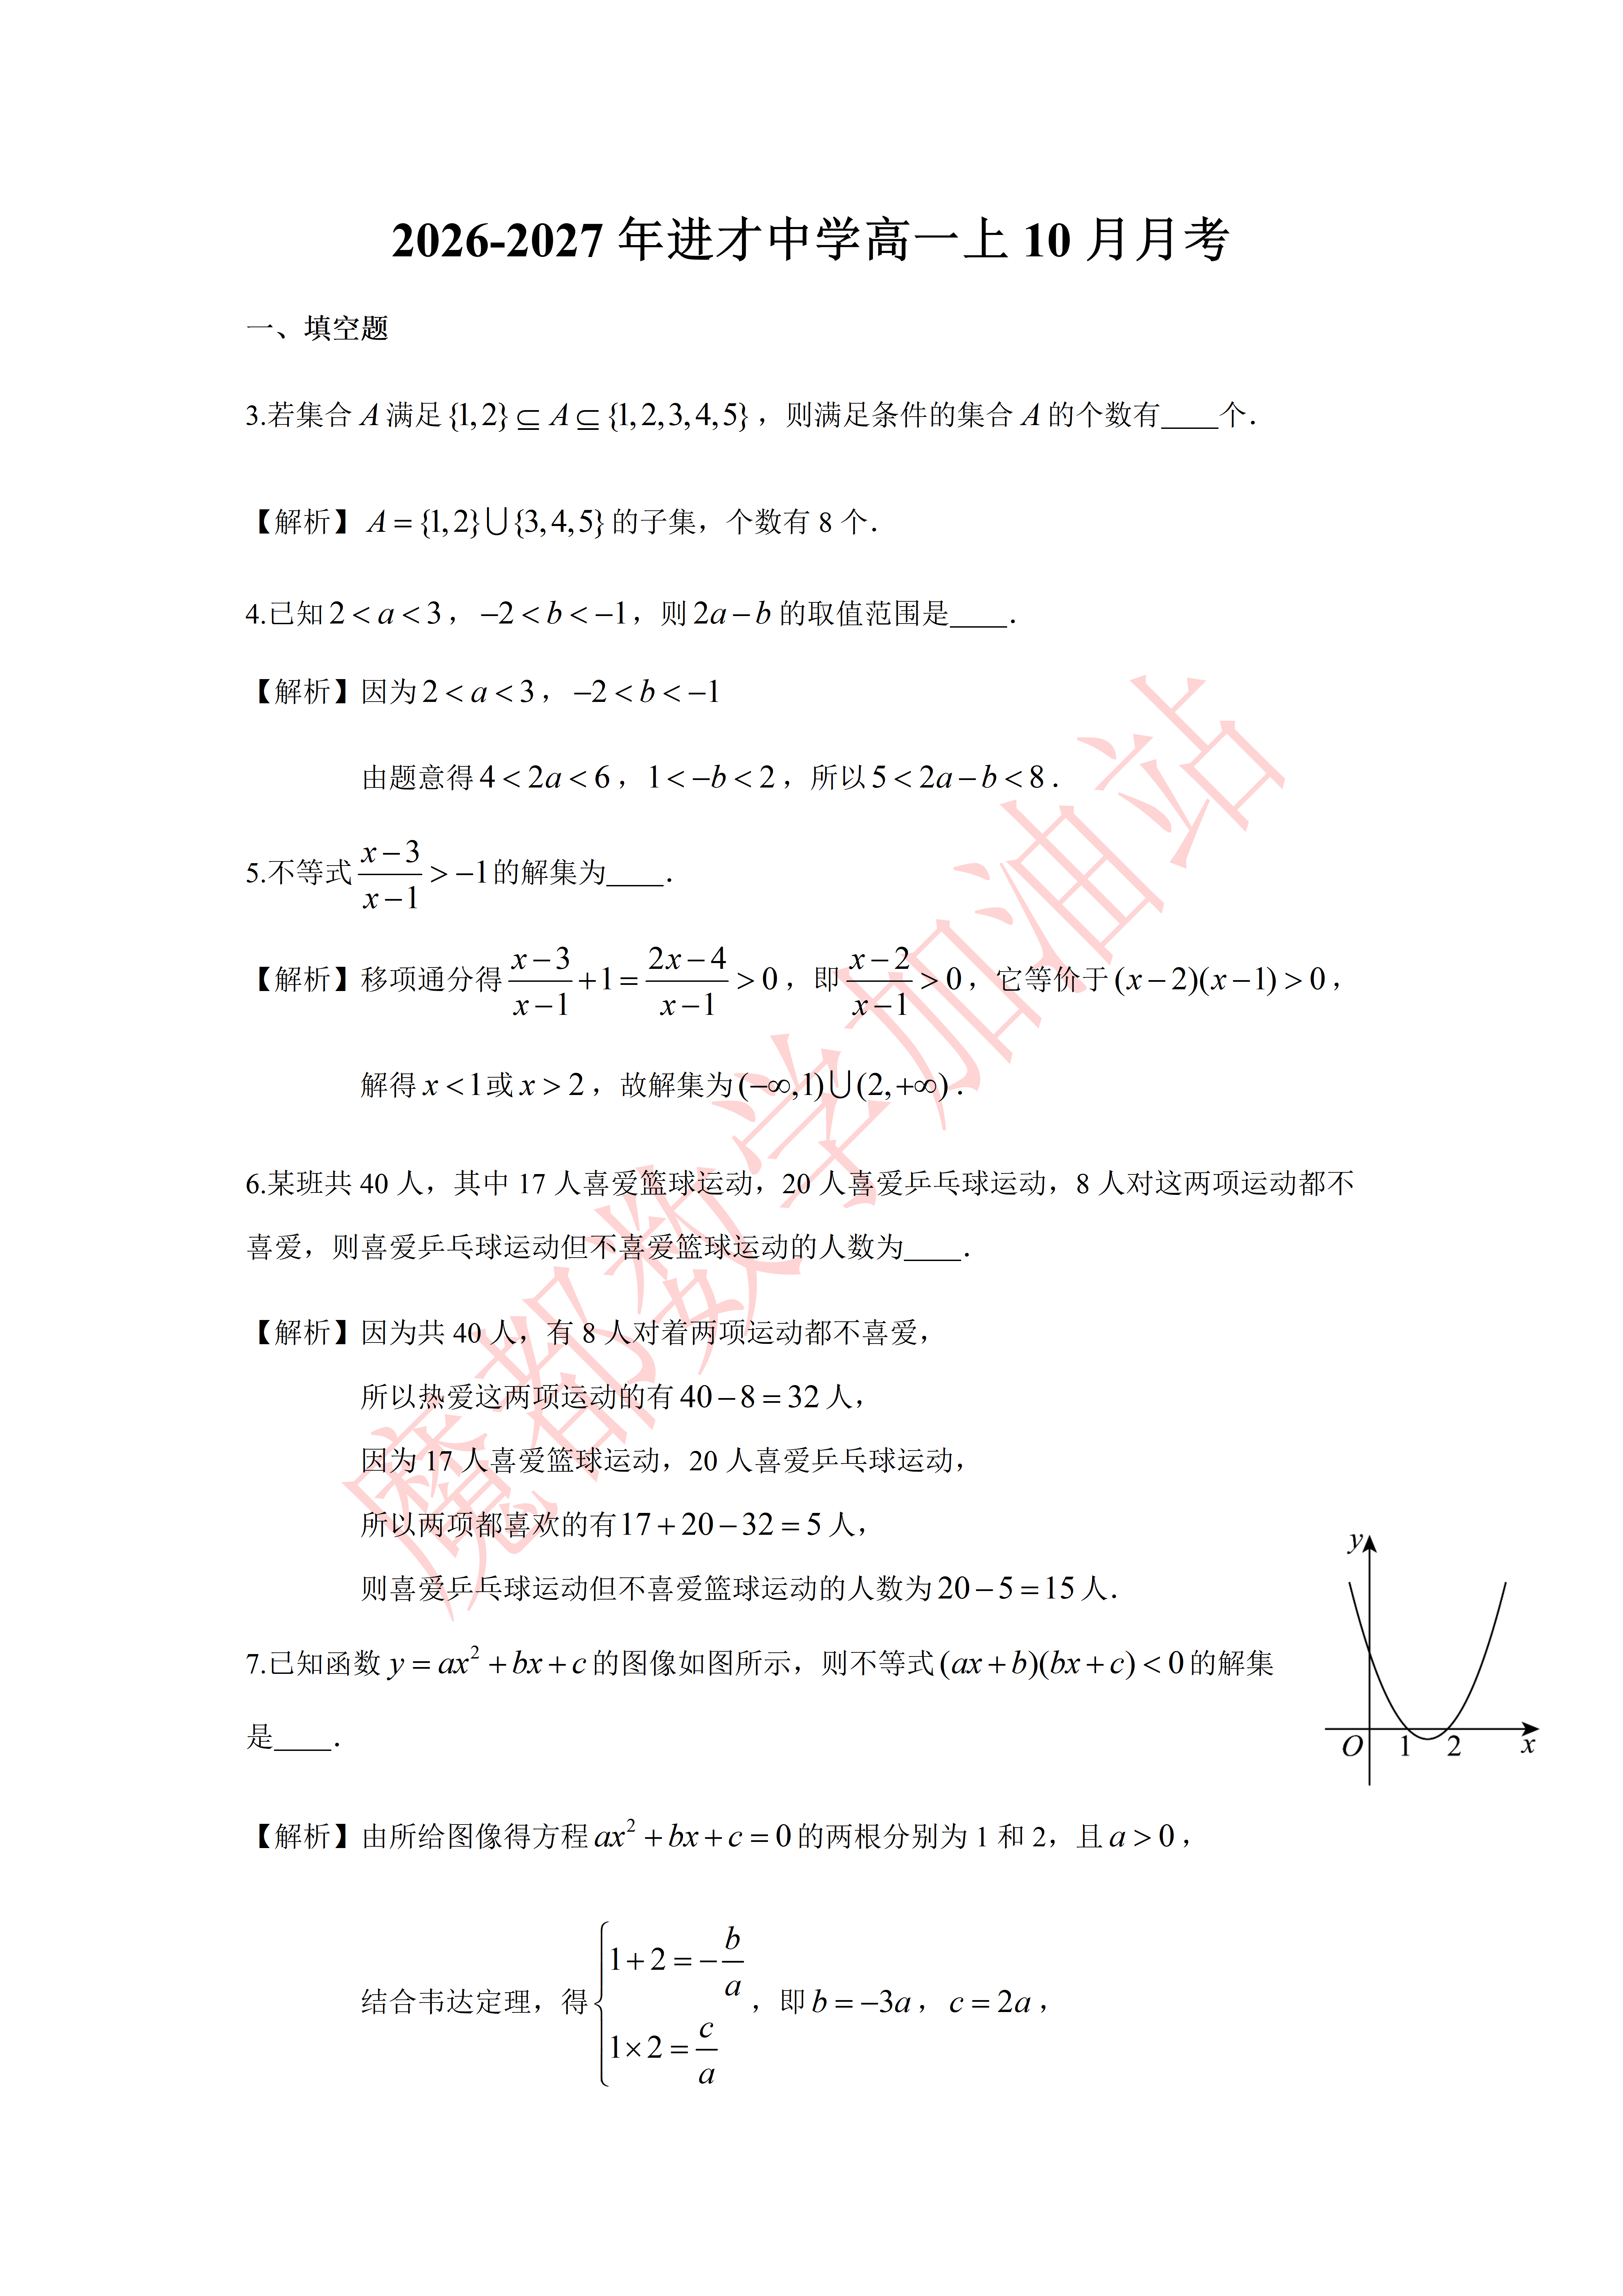
\includegraphics[width=.22\linewidth,trim=3879bp 1490bp 238bp 4492bp,clip]{../原图/高一60_进才中学_10月月考/01.png}
\end{center}

\ifanswer
\solbegin
\step{由所给图像得方程 $ax^2+bx+c=0$ 的两根分别为 1 和 2，且 $a>0$，}
\step{结合韦达定理，得 $\begin{cases}1+2=-\dfrac ba\\ 1\times2=\dfrac ca\end{cases}$，即 $b=-3a$，$c=2a$，}
\step{所以不等式 $(ax+b)(bx+c)<0$ 即 $(ax-3a)(-3ax+2a)<0$，}
\step{化简得 $(x-3)(3x-2)>0$，解得 $x<\dfrac23$ 或 $x>3$，}
\step{所以不等式 $(ax+b)(bx+c)<0$ 的解集是 $(-\infty,\dfrac23)\cup(3,+\infty)$.}
\solend
\fi

\item 已知集合 $A=\{x\mid ax=6\}$，满足 $A\subseteq\Z$，则整数 $a$ 的所有可能取值有\blankline[4.4em]个.

\ifanswer
\solbegin
\step{当 $a=0$ 时，$A=\varnothing$，而 $\varnothing\subseteq\Z$，满足题意，}
\step{当 $a\neq0$ 时，$A=\left\{\dfrac6a\right\}$，要使 $A\subseteq\Z$，则 $\dfrac6a\in\Z$，所以 $a=\pm1,\pm2,\pm3,\pm6$，}
\step{综上，整数 $a$ 的可能取值为 0，$\pm1$，$\pm2$，$\pm3$，$\pm6$，共 9 个.}
\solend
\fi

\item 设关于 $x$ 的方程 $x^2+kx+n=0$ 有两个不同实根 $x_1$、$x_2$，且 $\dfrac1{x_1}+\dfrac1{x_2}=2$，则实数 $n$ 的取值范围是\blankline[4.4em].

\ifanswer
\solbegin
\step{由于方程 $x^2+kx+n=0$ 有两个不同实根 $x_1$、$x_2$，}
\step{因此 $\Delta=k^2-4n>0$，$x_1+x_2=-k$，$x_1x_2=n$，}
\step{由 $\dfrac1{x_1}+\dfrac1{x_2}=\dfrac{x_1+x_2}{x_1x_2}=\dfrac{-k}{n}=2$，得 $k=-2n$，}
\step{因此 $\Delta=k^2-4n=4n^2-4n>0$，解得 $n<0$ 或 $n>1$，}
\step{则实数 $n$ 的取值范围是 $(-\infty,0)\cup(1,+\infty)$.}
\solend
\fi

\item 某船从甲地沿河顺流航行 $75\mathrm{km}$，到达乙码头，停留 $30\mathrm{min}$ 后再逆流航行 $126\mathrm{km}$ 到达丙地，若水流速度为 $4\mathrm{km/h}$，且该船要在 $5\mathrm{h}$ 内完成航行任务，那么船的速度至少达到\blankline[4.4em]$\mathrm{km/h}$.

\ifanswer
\solbegin
\step{设该轮船在静水中的速度是 $x$ 千米/小时，水流速度是 4 千米/小时，}
\step{由题意得 $\dfrac{75}{4+x}+0.5+\dfrac{126}{x-4}\leqslant5$，即 $9x^2-402x-552\geqslant0$，解得 $x\geqslant46$，}
\step{答：该船的速度至少是 46 千米/小时.}
\solend
\fi

\item 设实数 $a,b,c$ 满足 $a^2+b^2\leqslant c<1$，则 $a+\dfrac12b+c$ 的最小值为\blankline[4.4em].

\ifanswer
\solbegin
\step{因为 $c\geqslant a^2+b^2$，}
\step{所以 $a+\dfrac12b+c\geqslant a+\dfrac12b+a^2+b^2=\left(a+\dfrac12\right)^2+\left(b+\dfrac14\right)^2-\dfrac5{16}\geqslant-\dfrac5{16}$，}
\step{当 $a=-\dfrac12,b=-\dfrac14,c=a^2+b^2=\dfrac5{16}$（此时 $c<1$ 成立）时取到等号，}
\step{故最小值为 $-\dfrac5{16}$.}
\solend
\fi

\item 已知集合 $A=\{x\in\N^*\mid1\leqslant x\leqslant2026\}$. 设集合 $B=\{b_1,b_2,b_3,\cdots,b_n\}$ 满足 $B\subseteq A$，且对任意的 $b_i$、$b_j$、$b_k\in B(i$、$j$、$k\in\{1,2,3,\cdots,n\})$，存在 $m\in\N^*$，使得 $b_i+b_j+b_k=39m$，则 $n$ 的最大值为\blankline[4.4em].

\ifanswer
\solbegin
\step{因为 $39=1\times39=3\times13$，所以 $n$ 的最大值大于 3，}
\step{若对任意的 $b_i$、$b_j$、$b_k\in B$，存在 $m\in\N^*$，使得 $b_i+b_j+b_k=39m$，}
\step{则集合 $B$ 的元素除以 39 的余数均为 0 或均为 13 或均为 26，}
\step{即 $B=\{39,78,\cdots,39n\}$ 或 $B=\{13,52,\cdots,39n-26\}$}
\step{或 $B=\{26,65,\cdots,39n-13\}$，}
\step{若 $B=\{39,78,\cdots,39n\}$，则 $39n\leqslant2026$，}
\step{解得 $n\leqslant\dfrac{2026}{39}\in(51,52)$，此时 $n$ 的最大值为 51；}
\step{若 $B=\{13,52,\cdots,39n-26\}$，则 $39n-26\leqslant2026$，}
\step{解得 $n\leqslant\dfrac{684}{13}\in(52,53)$，此时 $n$ 的最大值为 52；}
\step{若 $B=\{26,65,\cdots,39n-13\}$，则 $39n-13\leqslant2026$，}
\step{解得 $n\leqslant\dfrac{2039}{39}\in(52,53)$，此时 $n$ 的最大值为 52；}
\step{综上，$n$ 的最大值为 52.}
\solend
\fi

\end{enumerate}

\bigsec{二、选择题}

\begin{enumerate}
\setcounter{enumi}{12}

% 第 13 题原卷无【答案】/【解析】段，答案“B”直接印在题干括号内，
% 按 高一53 第 13 题的成例括号留空、答案另提为 \ans{}（见文件头）
\item 已知 $a$、$b\in\R$，则“$|a|>|b|$”是“$a>|b|$”的\mbox{（\quad）}

\keepwithprev
A. 充分不必要条件\qquad B. 必要不充分条件

C. 充要条件\qquad D. 既不充分也不必要条件

\ifanswer
\ans{$B$}
\fi

\item 如果关于 $x$ 的一元二次方程 $x^2+2mx+(m+2)=0$ 有一正根一负根，那么 $m$ 的取值范围为\mbox{（\quad）}

\keepwithprev
A. $(-2,-1)$\qquad B. $(-1,2)$

C. $(-\infty,-1)\cup(2,+\infty)$\qquad D. $(-\infty,-2)$

\ifanswer
\solbegin
\step{设两根为 $x_1,x_2$，方程有一正根一负根，则 $\begin{cases}x_1x_2=m+2<0\\ \Delta=4m^2-4(m+2)>0\end{cases}$，}
\step{解得 $m<-2$，故选 $D$.}
\solend
\fi

\item 若不等式 $|3x-a|\leqslant x+2$ 的解集包含集合 $[0,1]$，则实数 $a$ 的取值范围为\mbox{（\quad）}

\keepwithprev
A. $[0,2]$\qquad B. $[0,1]$

C. $[1,2]$\qquad D. $(1,2)$

\ifanswer
\solbegin
% 原卷“法一：”“法二：”排红色加粗（全卷唯一红字），本稿按全稿子题标号样式排 \stepm
% （详见文件头“与原卷的排版差异”⑦）
\stepm{法一：}{不等式 $|3x-a|\leqslant x+2$ 化为 $2x-2\leqslant a\leqslant4x+2$，}
% 原卷此句缺动词（疑漏“对”字），照录未改（见文件头“原卷存疑”④）
\step{$[0,1]$ 使 $2x-2\leqslant a\leqslant4x+2$ 成立，则 $0\leqslant a\leqslant2$，故选 $A$.}
\stepm{法二：}{将两边平方整理得 $8x^2-(6a+4)x+a^2-4\leqslant0$ 对 $[0,1]$ 恒成立，}
\step{则有 $\begin{cases}a^2-4\leqslant0\\ a^2-6a\leqslant0\end{cases}$，解得 $0\leqslant a\leqslant2$，故选 $A$.}
\solend
\fi

\item 数学组 Y 老师在白纸上写下以下四个命题：

①这四个命题中至少有一个是真的；②这四个命题中至少有两个是真的；

③这四个命题中至少有两个是假的；④这四个命题中至少有一个是假的；

每个命题非真即假. 问 Y 老师在纸上写的假命题有几个？\mbox{（\quad）}

\keepwithprev
A. 0\qquad B. 1

C. 2\qquad D. 3

\ifanswer
\solbegin
\step{设四个命题中真命题的个数为 $t$，则①真 $\iff t\geqslant1$，②真 $\iff t\geqslant2$，}
\step{③真 $\iff t\leqslant2$，④真 $\iff t\leqslant3$.}
\step{逐一检验：$t=0$ 时③④为真，应为 $t=2$，矛盾；}
\step{$t=1$ 时①③④为真，应为 $t=3$，矛盾；}
\step{$t=2$ 时四个命题全为真，应为 $t=4$，矛盾；}
\step{$t=3$ 时①②④为真、③为假，恰有 3 个真命题，符合；}
\step{$t=4$ 时①②为真，应为 $t=2$，矛盾.}
\step{所以恰有 1 个假命题，故选 $B$.}
\solend
\fi

\end{enumerate}

\bigsec{三、解答题}

\begin{enumerate}
\setcounter{enumi}{16}

\item 已知：$x\in\R$，$a=x^2-1$，$b=4x+5$. 求证：$a$、$b$ 中至少有一个大于等于 0.

\ifanswer
\solbegin
\step{假设 $a$、$b$ 都小于 0，即 $a<0$，$b<0$，则 $a+b<0$.}
\step{又 $a+b=x^2-1+4x+5=x^2+4x+4=(x+2)^2\geqslant0$，}
\step{这与假设所得 $a+b<0$ 矛盾，故假设不成立，}
\step{所以 $a$、$b$ 中至少有一个大于等于 0.}
\solend
\fi

\ansspace[6]

% 原卷 A、B 两个集合定义之间排半角逗号“,”（5 倍放大核，右侧字距 19px，与全卷全角“，”的 65—79px 字距判然有别）；
% 本稿原误抄为全角“，”——已照录原卷半角（见文件头“与原卷的排版差异”⑤）
\item 已知集合 $A=\{x\mid4\leqslant x\leqslant12\}$,$B=\{x\mid a\leqslant x\leqslant2a+1\}$.

（1）若 $a=2$，求 $\overline A\cap B$；

（2）已知 $A\cup B=A$，求实数 $a$ 的取值范围.

\ifanswer
\solbegin
\stepm{(1)}{当 $a=2$ 时，$B=\{x\mid2\leqslant x\leqslant5\}$，}
\step{而 $A=\{x\mid4\leqslant x\leqslant12\}$，则 $\overline A=(-\infty,4)\cup(12,+\infty)$，所以 $\overline A\cap B=[2,4)$.}
\stepm{(2)}{$A\cup B=A$ 即 $B\subseteq A$.}
\stepm{①}{当 $B=\varnothing$ 时，$a>2a+1$，即 $a<-1$，符合；}
\stepm{②}{当 $B\neq\varnothing$ 时，需 $a\leqslant2a+1$ 且 $a\geqslant4$ 且 $2a+1\leqslant12$，即 $4\leqslant a\leqslant\dfrac{11}2$.}
\step{综上，$a$ 的取值范围是 $(-\infty,-1)\cup\left[4,\dfrac{11}2\right]$.}
\solend
\fi

\ansspace[8]

\item （1）若关于 $x$ 的不等式 $ax^2-3x+2<0$ 的解集不是空集，求实数 $a$ 的取值范围；

（2）求关于 $x$ 的不等式 $ax^2-3x+2>ax-1$ 的解集.

\ifanswer
\solbegin
\stepm{(1)}{若 $a>0$，关于 $x$ 的不等式 $ax^2-3x+2<0$ 的解集不空，}
\step{所以一元二次方程 $ax^2-3x+2=0$ 的判别式大于零，}
\step{即 $(-3)^2-8a>0\Rightarrow a<\dfrac98$，结合 $a>0$ 得 $0<a<\dfrac98$；}
\step{若 $a\leqslant0$，则关于 $x$ 的不等式 $ax^2-3x+2<0$ 的解集不是空集；}
\step{综上，实数 $a$ 的取值范围是 $\left(-\infty,\dfrac98\right)$.}
\stepm{(2)}{$ax^2-3x+2>ax-1\Rightarrow ax^2-(a+3)x+3>0\Rightarrow(ax-3)(x-1)>0$，}
\step{当 $a=0$ 时，不等式为 $x-1<0$，不等式的解集为 $\{x\mid x<1\}$；}
\step{当 $a<0$ 时，不等式化为 $\left(x-\dfrac3a\right)(x-1)<0$，}
\step{不等式的解集为 $\left\{x\mid\dfrac3a<x<1\right\}$，}
\step{当 $a>0$ 时，方程 $ax^2-3x+2=ax-1$ 的两个根分别为：$\dfrac3a,1$.}
\step{当 $a=3$ 时，两根相等，故不等式的解集为 $\{x\mid x\neq1\}$；}
\step{当 $a>3$ 时，$\dfrac3a<1$，不等式的解集为 $\left\{x\mid x<\dfrac3a\right.$ 或 $\left.x>1\right\}$；}
\step{当 $0<a<3$ 时，$\dfrac3a>1$，不等式的解集为 $\left\{x\mid x<1\right.$ 或 $\left.x>\dfrac3a\right\}$；}
\step{综上所述，当 $a<0$ 时，不等式的解集为 $\left\{x\mid\dfrac3a<x<1\right\}$，}
\step{当 $a=0$ 时，不等式的解集为 $\{x\mid x<1\}$，}
\step{当 $0<a<3$ 时，不等式的解集为 $\left\{x\mid x<1\right.$ 或 $\left.x>\dfrac3a\right\}$，}
\step{当 $a=3$ 时，不等式的解集为 $\{x\mid x\neq1\}$，}
\step{当 $a>3$ 时，不等式的解集为 $\left\{x\mid x<\dfrac3a\right.$ 或 $\left.x>1\right\}$.}
\solend
\fi

\ansspace[8]

\item 设命题 $p$：对任意 $x\in\R$，使得不等式 $mx^2-mx+2>0$ 恒成立；命题 $q$：存在 $0\leqslant x\leqslant3$，不等式 $2x-2\geqslant|m|$ 成立.

（1）若 $p$ 为真命题，求实数 $m$ 的取值范围；

（2）若 $p$、$q$ 有且只有一个是真命题，求实数 $m$ 的取值范围.

\ifanswer
\solbegin
\stepm{(1)}{因为 $p:\forall x\in\R$，$mx^2-mx+2>0$ 为真命题，}
\step{所以当 $m=0$ 时，不等式为 $2>0$，在 $\R$ 上恒成立，符合题意；}
\step{当 $m\neq0$ 时，$\begin{cases}m>0\\ \Delta=m^2-8m<0\end{cases}$，解得 $0<m<8$.}
\step{综上，实数 $m$ 的取值范围为 $[0,8)$.}
\stepm{(2)}{若 $q$ 为真命题，即 $q:\exists0\leqslant x\leqslant3$，$2x-2\geqslant|m|$，}
\step{则对于 $0\leqslant x\leqslant3$，$(2x-2)_{max}\geqslant|m|$.}
\step{由于 $0\leqslant x\leqslant3$，$2x-2\in[-2,4]$，所以 $|m|\leqslant4$，解得 $-4\leqslant m\leqslant4$，}
\step{又因为 $p$、$q$ 有且只有一个是真命题，}
\step{所以当 $p$ 真 $q$ 假时，$\begin{cases}0\leqslant m<8\\ m<-4\text{或}m>4\end{cases}$，解得 $4<m<8$；}
\step{当 $p$ 假 $q$ 真时，$\begin{cases}m<0\text{或}m\geqslant8\\ -4\leqslant m\leqslant4\end{cases}$，解得 $-4\leqslant m<0$；}
\step{综上，实数 $m$ 的取值范围为 $[-4,0)\cup(4,8)$.}
\solend
\fi

\ansspace[10]

\item 已知集合 $A=\{a_1,a_2,\cdots,a_k\}(k\geqslant2)$. 其中 $a_i\in\N^*(i=1,2,\cdots,k)$. 若对于任意的 $a\in A$，总有 $\dfrac1a\notin A$，则称集合 $A$ 具有性质 $P$. 由 $A$ 中的元素构成两个相应的集合：$S=\{(a,b)\mid a\in A,b\in A,ab\in A\}$，$T=\left\{(a,b)\mid a\in A,b\in A,\dfrac ab\in A\right\}$，其中 $(a,b)$ 是有序数对，集合 $S$ 和 $T$ 中的元素个数分别为 $m$ 和 $n$.

（1）检验集合 $\{2,3,6\}$ 与 $\{1,2,4\}$ 是否具有性质 $P$，并对其中具有性质 $P$ 的集合，写出相应的集合 $S$ 和 $T$；

（2）对任何具有性质 $P$ 的集合 $A$，$n$ 的最大值为多少？（直接写出答案，无需说明理由）；

% 原卷题干的小问编号跳号：印作 (1)(2)(4)，本稿照录 (4)、未改成 (3)（见文件头“原卷存疑”①）
（4）判断 $m$ 和 $n$ 的大小关系，并证明你的结论.

\ifanswer
\solbegin
\stepm{(1)}{因为 $\dfrac12\in\{1,2,4\}$，所以 $\{1,2,4\}$ 不具有性质 $P$；}
\step{因为 $\dfrac12\notin\{2,3,6\}$，$\dfrac13\notin\{2,3,6\}$，$\dfrac16\notin\{2,3,6\}$，所以 $\{2,3,6\}$ 具有性质 $P$.}
\step{$S=\{(2,3),(3,2)\}$，$T=\{(6,2),(6,3)\}$；}
\stepm{(2)}{因为对于任意的 $a\in A$，总有 $\dfrac1a\notin A$，所以 $1\notin A$，}
% 原卷此处印作“$\{(a_i,a_i)\}\in T$”，与上一句“$1\notin A$”及下文“最多为 $C_k^2$”的推理
% 均不自洽（应为“$\notin$”），已 8 倍放大确认无斜线；照录未改（见文件头“原卷存疑”③）
\step{从而 $\{(a_i,a_i)\}\in T(i=1,2,\cdots,k)$.}
\step{因为 $a\in A,b\in A,\dfrac ab\in A$，所以当 $i\neq j$ 时，}
\step{$(a_i,a_j)\in T$ 和 $(a_j,a_i)\in T(i,j=1,2,\cdots,k)$ 至多有一个成立，}
\step{所以集合 $T$ 中的元素个数最多为 $C_k^2=\dfrac{k(k-1)}2$，即 $n\leqslant\dfrac{k(k-1)}2$.}
% 原卷【解析】把第 (4) 问标作“(3)”（与题干跳号相应），本稿照录未改（见文件头“原卷存疑”①）
\stepm{(3)}{$m=n$，证明如下：}
\step{①设 $(a,b)\in T$，则 $a\in A,b\in A,\dfrac ab\in A$. 设 $c=\dfrac ab$，则 $a=bc$，}
\step{故 $b\in A$，$c\in A$，$bc\in A$，从而 $(b,c)\in S$，}
\step{即对 $\forall(a,b)\in T$，总 $\exists c$ 使 $(b,c)\in S$，从而 $n\leqslant m$.}
\step{②设 $(p,q)\in S$，则 $p\in A$，$q\in A$，$pq\in A$.}
\step{设 $r=pq$，则 $q=\dfrac rp$，故 $r\in A,p\in A,\dfrac rp\in A$，从而 $(r,p)\in T$，}
\step{即对 $\forall(p,q)\in S$，总 $\exists r$ 使 $(r,p)\in T$，从而 $m\leqslant n$.}
\step{由①②得 $m=n$.}
\solend
\fi

\ansspace*[10]

\end{enumerate}

\end{document}
"
%
% 原文链接：https://mp.weixin.qq.com/s/2ZLKB3IONEDhcUAfAAYE2A。
% 公众号“魔都数学加油站”作者破晓于 2026-10-14 22:15 发布。
% 原图 9 张（`原图/高一60_进才中学_10月月考/01..09.png`）：第 1—8 页 4762×6735，
% 第 9 页 2560×3620（同一篇内两档分辨率）。
%
% 卷首标题：照卷面印作“2026--2027 年进才中学高一上 10 月月考”（公众号标题中的“上海市”
% 卷面标题行没有，本稿照卷面），年份区间按全稿惯例排 en dash。原卷只有一行标题、无副标题。
%
% 篇幅与题号：原卷自第 3 题起编号（第 1、2 题不在本卷内）。填空题 3—12（10 题）、
% 选择题 13—16（4 题）、解答题 17—21（5 题），共 19 题。本稿沿用原节与原题号，
% 只改排为全稿统一的大节样式（原卷小节标题为“一、填空题”“二、选择题”“三、解答题”）。
%
% 讲评版：原卷每题下直接印【答案】或【解析】。**只印【解析】的 18 题**，本稿按全稿口径
% 收进答案版、不另提 \ans{}——第 14、15、16 题的结论写在解析末句（“故选 D／A／B”），
% 亦照录在解析内。**第 13 题原卷没有任何【答案】/【解析】段**，答案“B”直接印在题干括号内
% （“（ B ）”），本稿按 高一53 第 13 题的成例把括号留空、答案另提为 \ans{$B$}（见下）。
%
% 副标题：原卷未印副标题。本稿按“知识模块”口径标作“集合与常用逻辑用语、不等式”：
% 19 题中集合与常用逻辑用语 10 题（第 3、6、8、12、13、16、17、18、20、21 题，
% 含子集计数、韦恩图容斥、集合运算、命题与充要条件、反证法、新定义），
% 不等式 9 题（含不等式性质、分式不等式、二次函数与解集、韦达定理与判别式、
% 不等式应用、最值、根的分布、绝对值不等式恒成立、含参二次不等式：第 4、5、7、9、10、
% 11、14、15、19 题），两类均远超三分之一，故并标。口径同 高一46、高一47、高一48、
% 高一51—高一59。
%
% 与原卷的排版差异：
%   ① 原卷每题下直接印【答案】/【解析】，本稿按全稿惯例将答案与解析置于答案版，试卷版保持干净；
%   ② 原卷未印副标题，本稿按“知识模块”口径补出；
%   ③ 原卷填空横线约两个字宽，本稿按全稿惯例统一排 \blankline[4.4em]；
%   ④ 原卷实数集排斜体 $R$（第 13、17、20 题）、正整数集排 $N^*$（第 12、21 题）、
%      整数集排粗体 $\mathbf{Z}$（第 8 题），本稿按全稿惯例改用 $\R$、$\N^*$、$\Z$；
%      空集记号统一为 \varnothing；
%   ⑤ 原卷在数学式内多处用半角逗号（如 $x_1,x_2$、$a,b\in R$，以及第 18 题题干
%      $A=\{x\mid4\leqslant x\leqslant12\}$,$B=\{x\mid a\leqslant x\leqslant2a+1\}$ 之间的逗号），
%      均照录未强改（第 18 题题干那一处本稿首轮曾误作全角“，”，第二轮已订正）；
%      句末句点按全稿惯例排西文句点；
%   ⑥ 第 13 题印在题干括号内的答案“B”移入 \ans{}，见上；
%   ⑦ 第 15 题【解析】的“法一：”“法二：”标号原卷排**红色加粗**（全卷唯一的红字，2 处），
%      本稿按全稿子题标号样式排 \stepm{法一：}{…}、\stepm{法二：}{…}（加粗着色、不改黑色
%      基调），冒号照原卷排全角；
%   ⑧ 第 7 题的图像原卷排在题干右侧（与题干第 1 行同高），本稿居中排在题干之后；
%      图自原图第 01 页裁切（trim），不另存图片文件；
%   ⑨ 原卷第 10 题的长度与速度单位原卷排斜体（$75km$、$4km/h$ 等），本稿按全稿惯例
%      改排正体 $\mathrm{km}$、$\mathrm{km/h}$（同 高一56 第 13 题）；每道解答题原卷未留
%      作答空白，本稿按全稿惯例加 \ansspace。
%
% 原卷存疑（照录未改，见源码中该处上方注释）：
%   ① 第 21 题题干的小问编号**跳号**：印作 (1)(2)(4)，而紧随其后的【解析】按 (1)(2)(3) 写
%      —— 题干第 (4) 问实为第 (3) 问。本稿题干照录 (1)(2)(4)、解析照录 (3)，未改
%      （与 高一22 第 16 题“解析误标 (2)”同一处理）。
%   ② 第 6 题【解析】“有 8 人**对着**两项运动都不喜爱”，“对着”疑为“对这”之误，照录未改。
%   ③ 第 21(2) 题【解析】首行“所以 $1\notin A$，从而 $\{(a_i,a_i)\}\in T(i=1,2,\cdots,k)$”
%      —— 由 $1\notin A$ 应得 $(a_i,a_i)\notin T$（因 $a_i/a_i=1$），与紧随的“$T$ 中元素
%      个数最多为 $C_k^2$”这一推理亦只有“$\notin$”才自洽；原卷此处印作“$\in$”，
%      已 8 倍放大确认无斜线。**照录原卷的 $\in$、未改**。
%   ④ 第 15 题【解析】法一“$[0,1]$ 使 $2x-2\leqslant a\leqslant4x+2$ 成立”一句缺动词
%      （疑漏“对”字），照录未改。
%
\documentclass[a4paper,11pt]{article}
\usepackage{common}

\begin{document}

\examtitlest[3]{2026--2027 年进才中学高一上 10 月月考}{集合与常用逻辑用语、不等式}

\bigsec{一、填空题}

\begin{enumerate}
\setcounter{enumi}{2}

\item 若集合 $A$ 满足 $\{1,2\}\subseteq A\subseteq\{1,2,3,4,5\}$，则满足条件的集合 $A$ 的个数有\blankline[4.4em]个.

\ifanswer
\solbegin
\step{$A=\{1,2\}\cup\{3,4,5\}$ 的子集，个数有 8 个.}
\solend
\fi

\item 已知 $2<a<3$，$-2<b<-1$，则 $2a-b$ 的取值范围是\blankline[4.4em].

\ifanswer
\solbegin
\step{因为 $2<a<3$，$-2<b<-1$，}
\step{由题意得 $4<2a<6$，$1<-b<2$，所以 $5<2a-b<8$.}
\solend
\fi

\item 不等式 $\dfrac{x-3}{x-1}>-1$ 的解集为\blankline[4.4em].

\ifanswer
\solbegin
\step{移项通分得 $\dfrac{x-3}{x-1}+1=\dfrac{2x-4}{x-1}>0$，即 $\dfrac{x-2}{x-1}>0$，它等价于 $(x-2)(x-1)>0$，}
\step{解得 $x<1$ 或 $x>2$，故解集为 $(-\infty,1)\cup(2,+\infty)$.}
\solend
\fi

\item 某班共 40 人，其中 17 人喜爱篮球运动，20 人喜爱乒乓球运动，8 人对这两项运动都不喜爱，则喜爱乒乓球运动但不喜爱篮球运动的人数为\blankline[4.4em].

\ifanswer
\solbegin
% 原卷作“对着两项运动都不喜爱”（疑为“对这”之误），照录未改（见文件头“原卷存疑”②）
\step{因为共 40 人，有 8 人对着两项运动都不喜爱，}
\step{所以热爱这两项运动的有 $40-8=32$ 人，}
\step{因为 17 人喜爱篮球运动，20 人喜爱乒乓球运动，}
\step{所以两项都喜欢的有 $17+20-32=5$ 人，}
\step{则喜爱乒乓球运动但不喜爱篮球运动的人数为 $20-5=15$ 人.}
\solend
\fi

\item 已知函数 $y=ax^2+bx+c$ 的图像如图所示，则不等式 $(ax+b)(bx+c)<0$ 的解集是\blankline[4.4em].

% 原图第 01 页题干右侧的图像直接裁取。裁框取图外框 x 3887–4516、y 4500–5237
% （四周各留约 8px），trim=左 3879bp／下 1490bp／右 238bp／上 4492bp
% （页宽 4762、页高 6735）。
\begin{center}
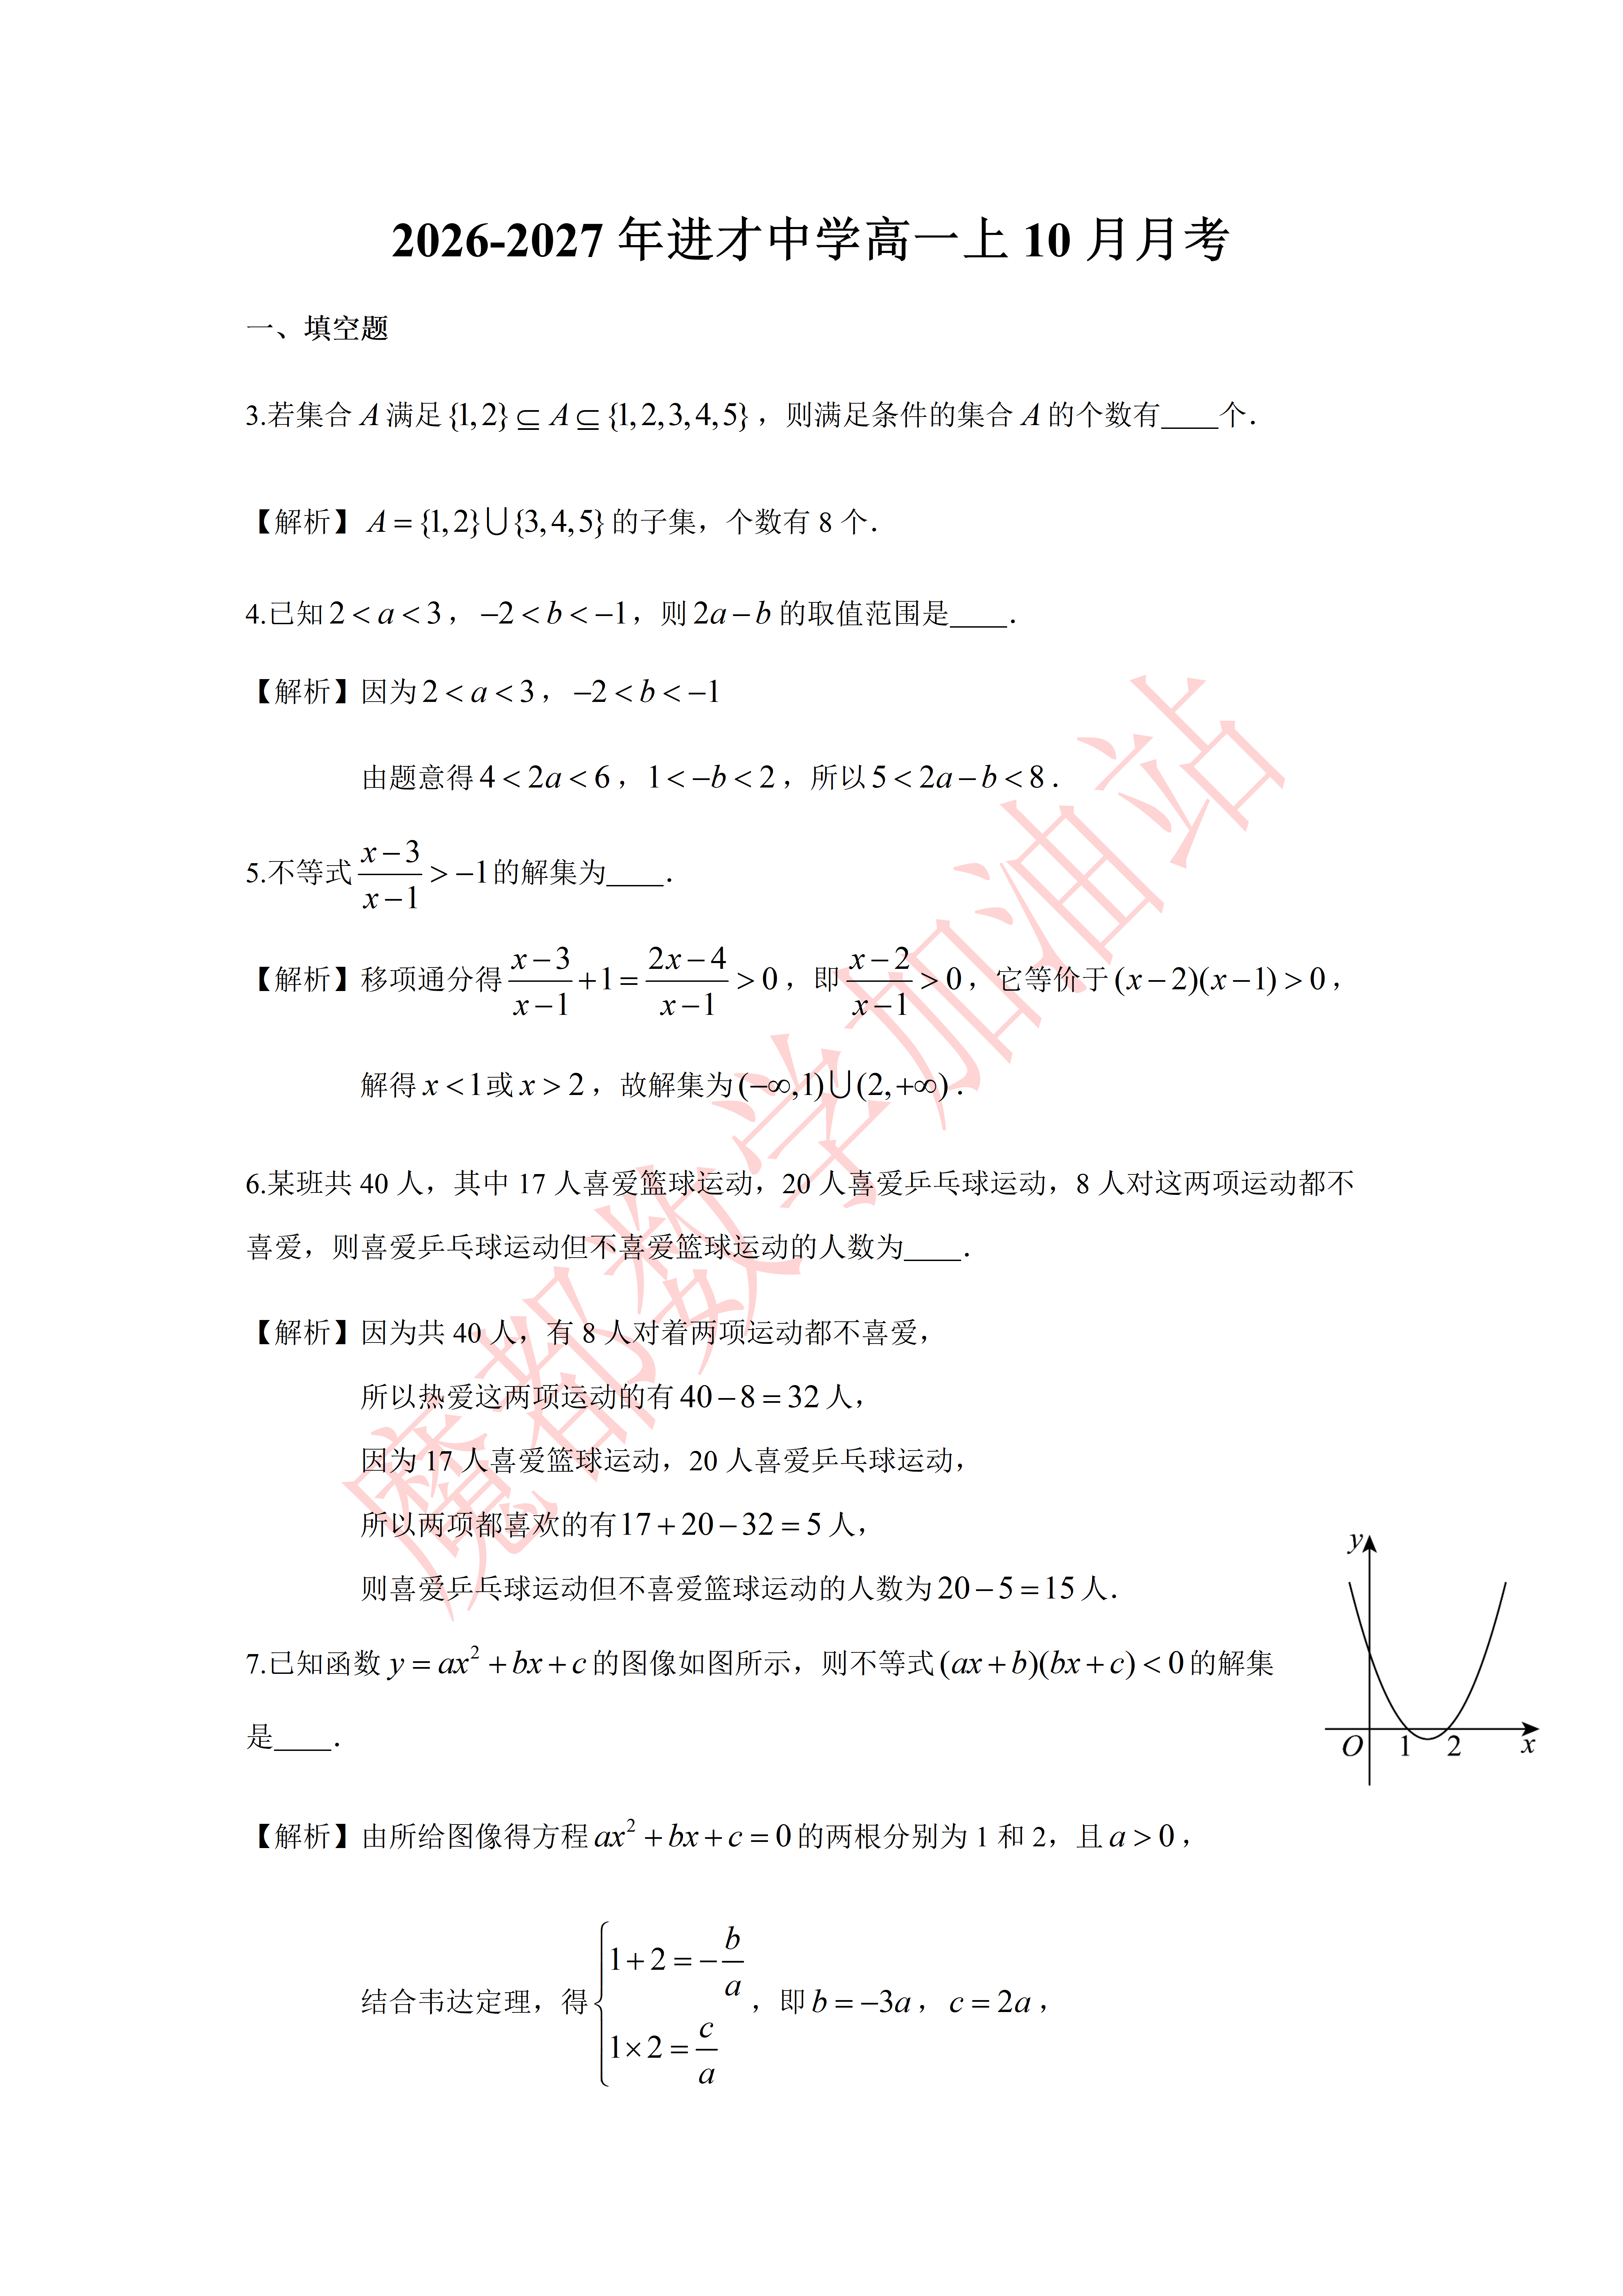
\includegraphics[width=.22\linewidth,trim=3879bp 1490bp 238bp 4492bp,clip]{../原图/高一60_进才中学_10月月考/01.png}
\end{center}

\ifanswer
\solbegin
\step{由所给图像得方程 $ax^2+bx+c=0$ 的两根分别为 1 和 2，且 $a>0$，}
\step{结合韦达定理，得 $\begin{cases}1+2=-\dfrac ba\\ 1\times2=\dfrac ca\end{cases}$，即 $b=-3a$，$c=2a$，}
\step{所以不等式 $(ax+b)(bx+c)<0$ 即 $(ax-3a)(-3ax+2a)<0$，}
\step{化简得 $(x-3)(3x-2)>0$，解得 $x<\dfrac23$ 或 $x>3$，}
\step{所以不等式 $(ax+b)(bx+c)<0$ 的解集是 $(-\infty,\dfrac23)\cup(3,+\infty)$.}
\solend
\fi

\item 已知集合 $A=\{x\mid ax=6\}$，满足 $A\subseteq\Z$，则整数 $a$ 的所有可能取值有\blankline[4.4em]个.

\ifanswer
\solbegin
\step{当 $a=0$ 时，$A=\varnothing$，而 $\varnothing\subseteq\Z$，满足题意，}
\step{当 $a\neq0$ 时，$A=\left\{\dfrac6a\right\}$，要使 $A\subseteq\Z$，则 $\dfrac6a\in\Z$，所以 $a=\pm1,\pm2,\pm3,\pm6$，}
\step{综上，整数 $a$ 的可能取值为 0，$\pm1$，$\pm2$，$\pm3$，$\pm6$，共 9 个.}
\solend
\fi

\item 设关于 $x$ 的方程 $x^2+kx+n=0$ 有两个不同实根 $x_1$、$x_2$，且 $\dfrac1{x_1}+\dfrac1{x_2}=2$，则实数 $n$ 的取值范围是\blankline[4.4em].

\ifanswer
\solbegin
\step{由于方程 $x^2+kx+n=0$ 有两个不同实根 $x_1$、$x_2$，}
\step{因此 $\Delta=k^2-4n>0$，$x_1+x_2=-k$，$x_1x_2=n$，}
\step{由 $\dfrac1{x_1}+\dfrac1{x_2}=\dfrac{x_1+x_2}{x_1x_2}=\dfrac{-k}{n}=2$，得 $k=-2n$，}
\step{因此 $\Delta=k^2-4n=4n^2-4n>0$，解得 $n<0$ 或 $n>1$，}
\step{则实数 $n$ 的取值范围是 $(-\infty,0)\cup(1,+\infty)$.}
\solend
\fi

\item 某船从甲地沿河顺流航行 $75\mathrm{km}$，到达乙码头，停留 $30\mathrm{min}$ 后再逆流航行 $126\mathrm{km}$ 到达丙地，若水流速度为 $4\mathrm{km/h}$，且该船要在 $5\mathrm{h}$ 内完成航行任务，那么船的速度至少达到\blankline[4.4em]$\mathrm{km/h}$.

\ifanswer
\solbegin
\step{设该轮船在静水中的速度是 $x$ 千米/小时，水流速度是 4 千米/小时，}
\step{由题意得 $\dfrac{75}{4+x}+0.5+\dfrac{126}{x-4}\leqslant5$，即 $9x^2-402x-552\geqslant0$，解得 $x\geqslant46$，}
\step{答：该船的速度至少是 46 千米/小时.}
\solend
\fi

\item 设实数 $a,b,c$ 满足 $a^2+b^2\leqslant c<1$，则 $a+\dfrac12b+c$ 的最小值为\blankline[4.4em].

\ifanswer
\solbegin
\step{因为 $c\geqslant a^2+b^2$，}
\step{所以 $a+\dfrac12b+c\geqslant a+\dfrac12b+a^2+b^2=\left(a+\dfrac12\right)^2+\left(b+\dfrac14\right)^2-\dfrac5{16}\geqslant-\dfrac5{16}$，}
\step{当 $a=-\dfrac12,b=-\dfrac14,c=a^2+b^2=\dfrac5{16}$（此时 $c<1$ 成立）时取到等号，}
\step{故最小值为 $-\dfrac5{16}$.}
\solend
\fi

\item 已知集合 $A=\{x\in\N^*\mid1\leqslant x\leqslant2026\}$. 设集合 $B=\{b_1,b_2,b_3,\cdots,b_n\}$ 满足 $B\subseteq A$，且对任意的 $b_i$、$b_j$、$b_k\in B(i$、$j$、$k\in\{1,2,3,\cdots,n\})$，存在 $m\in\N^*$，使得 $b_i+b_j+b_k=39m$，则 $n$ 的最大值为\blankline[4.4em].

\ifanswer
\solbegin
\step{因为 $39=1\times39=3\times13$，所以 $n$ 的最大值大于 3，}
\step{若对任意的 $b_i$、$b_j$、$b_k\in B$，存在 $m\in\N^*$，使得 $b_i+b_j+b_k=39m$，}
\step{则集合 $B$ 的元素除以 39 的余数均为 0 或均为 13 或均为 26，}
\step{即 $B=\{39,78,\cdots,39n\}$ 或 $B=\{13,52,\cdots,39n-26\}$}
\step{或 $B=\{26,65,\cdots,39n-13\}$，}
\step{若 $B=\{39,78,\cdots,39n\}$，则 $39n\leqslant2026$，}
\step{解得 $n\leqslant\dfrac{2026}{39}\in(51,52)$，此时 $n$ 的最大值为 51；}
\step{若 $B=\{13,52,\cdots,39n-26\}$，则 $39n-26\leqslant2026$，}
\step{解得 $n\leqslant\dfrac{684}{13}\in(52,53)$，此时 $n$ 的最大值为 52；}
\step{若 $B=\{26,65,\cdots,39n-13\}$，则 $39n-13\leqslant2026$，}
\step{解得 $n\leqslant\dfrac{2039}{39}\in(52,53)$，此时 $n$ 的最大值为 52；}
\step{综上，$n$ 的最大值为 52.}
\solend
\fi

\end{enumerate}

\bigsec{二、选择题}

\begin{enumerate}
\setcounter{enumi}{12}

% 第 13 题原卷无【答案】/【解析】段，答案“B”直接印在题干括号内，
% 按 高一53 第 13 题的成例括号留空、答案另提为 \ans{}（见文件头）
\item 已知 $a$、$b\in\R$，则“$|a|>|b|$”是“$a>|b|$”的\mbox{（\quad）}

\keepwithprev
A. 充分不必要条件\qquad B. 必要不充分条件

C. 充要条件\qquad D. 既不充分也不必要条件

\ifanswer
\ans{$B$}
\fi

\item 如果关于 $x$ 的一元二次方程 $x^2+2mx+(m+2)=0$ 有一正根一负根，那么 $m$ 的取值范围为\mbox{（\quad）}

\keepwithprev
A. $(-2,-1)$\qquad B. $(-1,2)$

C. $(-\infty,-1)\cup(2,+\infty)$\qquad D. $(-\infty,-2)$

\ifanswer
\solbegin
\step{设两根为 $x_1,x_2$，方程有一正根一负根，则 $\begin{cases}x_1x_2=m+2<0\\ \Delta=4m^2-4(m+2)>0\end{cases}$，}
\step{解得 $m<-2$，故选 $D$.}
\solend
\fi

\item 若不等式 $|3x-a|\leqslant x+2$ 的解集包含集合 $[0,1]$，则实数 $a$ 的取值范围为\mbox{（\quad）}

\keepwithprev
A. $[0,2]$\qquad B. $[0,1]$

C. $[1,2]$\qquad D. $(1,2)$

\ifanswer
\solbegin
% 原卷“法一：”“法二：”排红色加粗（全卷唯一红字），本稿按全稿子题标号样式排 \stepm
% （详见文件头“与原卷的排版差异”⑦）
\stepm{法一：}{不等式 $|3x-a|\leqslant x+2$ 化为 $2x-2\leqslant a\leqslant4x+2$，}
% 原卷此句缺动词（疑漏“对”字），照录未改（见文件头“原卷存疑”④）
\step{$[0,1]$ 使 $2x-2\leqslant a\leqslant4x+2$ 成立，则 $0\leqslant a\leqslant2$，故选 $A$.}
\stepm{法二：}{将两边平方整理得 $8x^2-(6a+4)x+a^2-4\leqslant0$ 对 $[0,1]$ 恒成立，}
\step{则有 $\begin{cases}a^2-4\leqslant0\\ a^2-6a\leqslant0\end{cases}$，解得 $0\leqslant a\leqslant2$，故选 $A$.}
\solend
\fi

\item 数学组 Y 老师在白纸上写下以下四个命题：

①这四个命题中至少有一个是真的；②这四个命题中至少有两个是真的；

③这四个命题中至少有两个是假的；④这四个命题中至少有一个是假的；

每个命题非真即假. 问 Y 老师在纸上写的假命题有几个？\mbox{（\quad）}

\keepwithprev
A. 0\qquad B. 1

C. 2\qquad D. 3

\ifanswer
\solbegin
\step{设四个命题中真命题的个数为 $t$，则①真 $\iff t\geqslant1$，②真 $\iff t\geqslant2$，}
\step{③真 $\iff t\leqslant2$，④真 $\iff t\leqslant3$.}
\step{逐一检验：$t=0$ 时③④为真，应为 $t=2$，矛盾；}
\step{$t=1$ 时①③④为真，应为 $t=3$，矛盾；}
\step{$t=2$ 时四个命题全为真，应为 $t=4$，矛盾；}
\step{$t=3$ 时①②④为真、③为假，恰有 3 个真命题，符合；}
\step{$t=4$ 时①②为真，应为 $t=2$，矛盾.}
\step{所以恰有 1 个假命题，故选 $B$.}
\solend
\fi

\end{enumerate}

\bigsec{三、解答题}

\begin{enumerate}
\setcounter{enumi}{16}

\item 已知：$x\in\R$，$a=x^2-1$，$b=4x+5$. 求证：$a$、$b$ 中至少有一个大于等于 0.

\ifanswer
\solbegin
\step{假设 $a$、$b$ 都小于 0，即 $a<0$，$b<0$，则 $a+b<0$.}
\step{又 $a+b=x^2-1+4x+5=x^2+4x+4=(x+2)^2\geqslant0$，}
\step{这与假设所得 $a+b<0$ 矛盾，故假设不成立，}
\step{所以 $a$、$b$ 中至少有一个大于等于 0.}
\solend
\fi

\ansspace[6]

% 原卷 A、B 两个集合定义之间排半角逗号“,”（5 倍放大核，右侧字距 19px，与全卷全角“，”的 65—79px 字距判然有别）；
% 本稿原误抄为全角“，”——已照录原卷半角（见文件头“与原卷的排版差异”⑤）
\item 已知集合 $A=\{x\mid4\leqslant x\leqslant12\}$,$B=\{x\mid a\leqslant x\leqslant2a+1\}$.

（1）若 $a=2$，求 $\overline A\cap B$；

（2）已知 $A\cup B=A$，求实数 $a$ 的取值范围.

\ifanswer
\solbegin
\stepm{(1)}{当 $a=2$ 时，$B=\{x\mid2\leqslant x\leqslant5\}$，}
\step{而 $A=\{x\mid4\leqslant x\leqslant12\}$，则 $\overline A=(-\infty,4)\cup(12,+\infty)$，所以 $\overline A\cap B=[2,4)$.}
\stepm{(2)}{$A\cup B=A$ 即 $B\subseteq A$.}
\stepm{①}{当 $B=\varnothing$ 时，$a>2a+1$，即 $a<-1$，符合；}
\stepm{②}{当 $B\neq\varnothing$ 时，需 $a\leqslant2a+1$ 且 $a\geqslant4$ 且 $2a+1\leqslant12$，即 $4\leqslant a\leqslant\dfrac{11}2$.}
\step{综上，$a$ 的取值范围是 $(-\infty,-1)\cup\left[4,\dfrac{11}2\right]$.}
\solend
\fi

\ansspace[8]

\item （1）若关于 $x$ 的不等式 $ax^2-3x+2<0$ 的解集不是空集，求实数 $a$ 的取值范围；

（2）求关于 $x$ 的不等式 $ax^2-3x+2>ax-1$ 的解集.

\ifanswer
\solbegin
\stepm{(1)}{若 $a>0$，关于 $x$ 的不等式 $ax^2-3x+2<0$ 的解集不空，}
\step{所以一元二次方程 $ax^2-3x+2=0$ 的判别式大于零，}
\step{即 $(-3)^2-8a>0\Rightarrow a<\dfrac98$，结合 $a>0$ 得 $0<a<\dfrac98$；}
\step{若 $a\leqslant0$，则关于 $x$ 的不等式 $ax^2-3x+2<0$ 的解集不是空集；}
\step{综上，实数 $a$ 的取值范围是 $\left(-\infty,\dfrac98\right)$.}
\stepm{(2)}{$ax^2-3x+2>ax-1\Rightarrow ax^2-(a+3)x+3>0\Rightarrow(ax-3)(x-1)>0$，}
\step{当 $a=0$ 时，不等式为 $x-1<0$，不等式的解集为 $\{x\mid x<1\}$；}
\step{当 $a<0$ 时，不等式化为 $\left(x-\dfrac3a\right)(x-1)<0$，}
\step{不等式的解集为 $\left\{x\mid\dfrac3a<x<1\right\}$，}
\step{当 $a>0$ 时，方程 $ax^2-3x+2=ax-1$ 的两个根分别为：$\dfrac3a,1$.}
\step{当 $a=3$ 时，两根相等，故不等式的解集为 $\{x\mid x\neq1\}$；}
\step{当 $a>3$ 时，$\dfrac3a<1$，不等式的解集为 $\left\{x\mid x<\dfrac3a\right.$ 或 $\left.x>1\right\}$；}
\step{当 $0<a<3$ 时，$\dfrac3a>1$，不等式的解集为 $\left\{x\mid x<1\right.$ 或 $\left.x>\dfrac3a\right\}$；}
\step{综上所述，当 $a<0$ 时，不等式的解集为 $\left\{x\mid\dfrac3a<x<1\right\}$，}
\step{当 $a=0$ 时，不等式的解集为 $\{x\mid x<1\}$，}
\step{当 $0<a<3$ 时，不等式的解集为 $\left\{x\mid x<1\right.$ 或 $\left.x>\dfrac3a\right\}$，}
\step{当 $a=3$ 时，不等式的解集为 $\{x\mid x\neq1\}$，}
\step{当 $a>3$ 时，不等式的解集为 $\left\{x\mid x<\dfrac3a\right.$ 或 $\left.x>1\right\}$.}
\solend
\fi

\ansspace[8]

\item 设命题 $p$：对任意 $x\in\R$，使得不等式 $mx^2-mx+2>0$ 恒成立；命题 $q$：存在 $0\leqslant x\leqslant3$，不等式 $2x-2\geqslant|m|$ 成立.

（1）若 $p$ 为真命题，求实数 $m$ 的取值范围；

（2）若 $p$、$q$ 有且只有一个是真命题，求实数 $m$ 的取值范围.

\ifanswer
\solbegin
\stepm{(1)}{因为 $p:\forall x\in\R$，$mx^2-mx+2>0$ 为真命题，}
\step{所以当 $m=0$ 时，不等式为 $2>0$，在 $\R$ 上恒成立，符合题意；}
\step{当 $m\neq0$ 时，$\begin{cases}m>0\\ \Delta=m^2-8m<0\end{cases}$，解得 $0<m<8$.}
\step{综上，实数 $m$ 的取值范围为 $[0,8)$.}
\stepm{(2)}{若 $q$ 为真命题，即 $q:\exists0\leqslant x\leqslant3$，$2x-2\geqslant|m|$，}
\step{则对于 $0\leqslant x\leqslant3$，$(2x-2)_{max}\geqslant|m|$.}
\step{由于 $0\leqslant x\leqslant3$，$2x-2\in[-2,4]$，所以 $|m|\leqslant4$，解得 $-4\leqslant m\leqslant4$，}
\step{又因为 $p$、$q$ 有且只有一个是真命题，}
\step{所以当 $p$ 真 $q$ 假时，$\begin{cases}0\leqslant m<8\\ m<-4\text{或}m>4\end{cases}$，解得 $4<m<8$；}
\step{当 $p$ 假 $q$ 真时，$\begin{cases}m<0\text{或}m\geqslant8\\ -4\leqslant m\leqslant4\end{cases}$，解得 $-4\leqslant m<0$；}
\step{综上，实数 $m$ 的取值范围为 $[-4,0)\cup(4,8)$.}
\solend
\fi

\ansspace[10]

\item 已知集合 $A=\{a_1,a_2,\cdots,a_k\}(k\geqslant2)$. 其中 $a_i\in\N^*(i=1,2,\cdots,k)$. 若对于任意的 $a\in A$，总有 $\dfrac1a\notin A$，则称集合 $A$ 具有性质 $P$. 由 $A$ 中的元素构成两个相应的集合：$S=\{(a,b)\mid a\in A,b\in A,ab\in A\}$，$T=\left\{(a,b)\mid a\in A,b\in A,\dfrac ab\in A\right\}$，其中 $(a,b)$ 是有序数对，集合 $S$ 和 $T$ 中的元素个数分别为 $m$ 和 $n$.

（1）检验集合 $\{2,3,6\}$ 与 $\{1,2,4\}$ 是否具有性质 $P$，并对其中具有性质 $P$ 的集合，写出相应的集合 $S$ 和 $T$；

（2）对任何具有性质 $P$ 的集合 $A$，$n$ 的最大值为多少？（直接写出答案，无需说明理由）；

% 原卷题干的小问编号跳号：印作 (1)(2)(4)，本稿照录 (4)、未改成 (3)（见文件头“原卷存疑”①）
（4）判断 $m$ 和 $n$ 的大小关系，并证明你的结论.

\ifanswer
\solbegin
\stepm{(1)}{因为 $\dfrac12\in\{1,2,4\}$，所以 $\{1,2,4\}$ 不具有性质 $P$；}
\step{因为 $\dfrac12\notin\{2,3,6\}$，$\dfrac13\notin\{2,3,6\}$，$\dfrac16\notin\{2,3,6\}$，所以 $\{2,3,6\}$ 具有性质 $P$.}
\step{$S=\{(2,3),(3,2)\}$，$T=\{(6,2),(6,3)\}$；}
\stepm{(2)}{因为对于任意的 $a\in A$，总有 $\dfrac1a\notin A$，所以 $1\notin A$，}
% 原卷此处印作“$\{(a_i,a_i)\}\in T$”，与上一句“$1\notin A$”及下文“最多为 $C_k^2$”的推理
% 均不自洽（应为“$\notin$”），已 8 倍放大确认无斜线；照录未改（见文件头“原卷存疑”③）
\step{从而 $\{(a_i,a_i)\}\in T(i=1,2,\cdots,k)$.}
\step{因为 $a\in A,b\in A,\dfrac ab\in A$，所以当 $i\neq j$ 时，}
\step{$(a_i,a_j)\in T$ 和 $(a_j,a_i)\in T(i,j=1,2,\cdots,k)$ 至多有一个成立，}
\step{所以集合 $T$ 中的元素个数最多为 $C_k^2=\dfrac{k(k-1)}2$，即 $n\leqslant\dfrac{k(k-1)}2$.}
% 原卷【解析】把第 (4) 问标作“(3)”（与题干跳号相应），本稿照录未改（见文件头“原卷存疑”①）
\stepm{(3)}{$m=n$，证明如下：}
\step{①设 $(a,b)\in T$，则 $a\in A,b\in A,\dfrac ab\in A$. 设 $c=\dfrac ab$，则 $a=bc$，}
\step{故 $b\in A$，$c\in A$，$bc\in A$，从而 $(b,c)\in S$，}
\step{即对 $\forall(a,b)\in T$，总 $\exists c$ 使 $(b,c)\in S$，从而 $n\leqslant m$.}
\step{②设 $(p,q)\in S$，则 $p\in A$，$q\in A$，$pq\in A$.}
\step{设 $r=pq$，则 $q=\dfrac rp$，故 $r\in A,p\in A,\dfrac rp\in A$，从而 $(r,p)\in T$，}
\step{即对 $\forall(p,q)\in S$，总 $\exists r$ 使 $(r,p)\in T$，从而 $m\leqslant n$.}
\step{由①②得 $m=n$.}
\solend
\fi

\ansspace*[10]

\end{enumerate}

\end{document}
"
%
% 原文链接：https://mp.weixin.qq.com/s/2ZLKB3IONEDhcUAfAAYE2A。
% 公众号“魔都数学加油站”作者破晓于 2026-10-14 22:15 发布。
% 原图 9 张（`原图/高一60_进才中学_10月月考/01..09.png`）：第 1—8 页 4762×6735，
% 第 9 页 2560×3620（同一篇内两档分辨率）。
%
% 卷首标题：照卷面印作“2026--2027 年进才中学高一上 10 月月考”（公众号标题中的“上海市”
% 卷面标题行没有，本稿照卷面），年份区间按全稿惯例排 en dash。原卷只有一行标题、无副标题。
%
% 篇幅与题号：原卷自第 3 题起编号（第 1、2 题不在本卷内）。填空题 3—12（10 题）、
% 选择题 13—16（4 题）、解答题 17—21（5 题），共 19 题。本稿沿用原节与原题号，
% 只改排为全稿统一的大节样式（原卷小节标题为“一、填空题”“二、选择题”“三、解答题”）。
%
% 讲评版：原卷每题下直接印【答案】或【解析】。**只印【解析】的 18 题**，本稿按全稿口径
% 收进答案版、不另提 \ans{}——第 14、15、16 题的结论写在解析末句（“故选 D／A／B”），
% 亦照录在解析内。**第 13 题原卷没有任何【答案】/【解析】段**，答案“B”直接印在题干括号内
% （“（ B ）”），本稿按 高一53 第 13 题的成例把括号留空、答案另提为 \ans{$B$}（见下）。
%
% 副标题：原卷未印副标题。本稿按“知识模块”口径标作“集合与常用逻辑用语、不等式”：
% 19 题中集合与常用逻辑用语 10 题（第 3、6、8、12、13、16、17、18、20、21 题，
% 含子集计数、韦恩图容斥、集合运算、命题与充要条件、反证法、新定义），
% 不等式 9 题（含不等式性质、分式不等式、二次函数与解集、韦达定理与判别式、
% 不等式应用、最值、根的分布、绝对值不等式恒成立、含参二次不等式：第 4、5、7、9、10、
% 11、14、15、19 题），两类均远超三分之一，故并标。口径同 高一46、高一47、高一48、
% 高一51—高一59。
%
% 与原卷的排版差异：
%   ① 原卷每题下直接印【答案】/【解析】，本稿按全稿惯例将答案与解析置于答案版，试卷版保持干净；
%   ② 原卷未印副标题，本稿按“知识模块”口径补出；
%   ③ 原卷填空横线约两个字宽，本稿按全稿惯例统一排 \blankline[4.4em]；
%   ④ 原卷实数集排斜体 $R$（第 13、17、20 题）、正整数集排 $N^*$（第 12、21 题）、
%      整数集排粗体 $\mathbf{Z}$（第 8 题），本稿按全稿惯例改用 $\R$、$\N^*$、$\Z$；
%      空集记号统一为 \varnothing；
%   ⑤ 原卷在数学式内多处用半角逗号（如 $x_1,x_2$、$a,b\in R$，以及第 18 题题干
%      $A=\{x\mid4\leqslant x\leqslant12\}$,$B=\{x\mid a\leqslant x\leqslant2a+1\}$ 之间的逗号），
%      均照录未强改（第 18 题题干那一处本稿首轮曾误作全角“，”，第二轮已订正）；
%      句末句点按全稿惯例排西文句点；
%   ⑥ 第 13 题印在题干括号内的答案“B”移入 \ans{}，见上；
%   ⑦ 第 15 题【解析】的“法一：”“法二：”标号原卷排**红色加粗**（全卷唯一的红字，2 处），
%      本稿按全稿子题标号样式排 \stepm{法一：}{…}、\stepm{法二：}{…}（加粗着色、不改黑色
%      基调），冒号照原卷排全角；
%   ⑧ 第 7 题的图像原卷排在题干右侧（与题干第 1 行同高），本稿居中排在题干之后；
%      图自原图第 01 页裁切（trim），不另存图片文件；
%   ⑨ 原卷第 10 题的长度与速度单位原卷排斜体（$75km$、$4km/h$ 等），本稿按全稿惯例
%      改排正体 $\mathrm{km}$、$\mathrm{km/h}$（同 高一56 第 13 题）；每道解答题原卷未留
%      作答空白，本稿按全稿惯例加 \ansspace。
%
% 原卷存疑（照录未改，见源码中该处上方注释）：
%   ① 第 21 题题干的小问编号**跳号**：印作 (1)(2)(4)，而紧随其后的【解析】按 (1)(2)(3) 写
%      —— 题干第 (4) 问实为第 (3) 问。本稿题干照录 (1)(2)(4)、解析照录 (3)，未改
%      （与 高一22 第 16 题“解析误标 (2)”同一处理）。
%   ② 第 6 题【解析】“有 8 人**对着**两项运动都不喜爱”，“对着”疑为“对这”之误，照录未改。
%   ③ 第 21(2) 题【解析】首行“所以 $1\notin A$，从而 $\{(a_i,a_i)\}\in T(i=1,2,\cdots,k)$”
%      —— 由 $1\notin A$ 应得 $(a_i,a_i)\notin T$（因 $a_i/a_i=1$），与紧随的“$T$ 中元素
%      个数最多为 $C_k^2$”这一推理亦只有“$\notin$”才自洽；原卷此处印作“$\in$”，
%      已 8 倍放大确认无斜线。**照录原卷的 $\in$、未改**。
%   ④ 第 15 题【解析】法一“$[0,1]$ 使 $2x-2\leqslant a\leqslant4x+2$ 成立”一句缺动词
%      （疑漏“对”字），照录未改。
%
\documentclass[a4paper,11pt]{article}
\usepackage{common}

\begin{document}

\examtitlest[3]{2026--2027 年进才中学高一上 10 月月考}{集合与常用逻辑用语、不等式}

\bigsec{一、填空题}

\begin{enumerate}
\setcounter{enumi}{2}

\item 若集合 $A$ 满足 $\{1,2\}\subseteq A\subseteq\{1,2,3,4,5\}$，则满足条件的集合 $A$ 的个数有\blankline[4.4em]个.

\ifanswer
\solbegin
\step{$A=\{1,2\}\cup\{3,4,5\}$ 的子集，个数有 8 个.}
\solend
\fi

\item 已知 $2<a<3$，$-2<b<-1$，则 $2a-b$ 的取值范围是\blankline[4.4em].

\ifanswer
\solbegin
\step{因为 $2<a<3$，$-2<b<-1$，}
\step{由题意得 $4<2a<6$，$1<-b<2$，所以 $5<2a-b<8$.}
\solend
\fi

\item 不等式 $\dfrac{x-3}{x-1}>-1$ 的解集为\blankline[4.4em].

\ifanswer
\solbegin
\step{移项通分得 $\dfrac{x-3}{x-1}+1=\dfrac{2x-4}{x-1}>0$，即 $\dfrac{x-2}{x-1}>0$，它等价于 $(x-2)(x-1)>0$，}
\step{解得 $x<1$ 或 $x>2$，故解集为 $(-\infty,1)\cup(2,+\infty)$.}
\solend
\fi

\item 某班共 40 人，其中 17 人喜爱篮球运动，20 人喜爱乒乓球运动，8 人对这两项运动都不喜爱，则喜爱乒乓球运动但不喜爱篮球运动的人数为\blankline[4.4em].

\ifanswer
\solbegin
% 原卷作“对着两项运动都不喜爱”（疑为“对这”之误），照录未改（见文件头“原卷存疑”②）
\step{因为共 40 人，有 8 人对着两项运动都不喜爱，}
\step{所以热爱这两项运动的有 $40-8=32$ 人，}
\step{因为 17 人喜爱篮球运动，20 人喜爱乒乓球运动，}
\step{所以两项都喜欢的有 $17+20-32=5$ 人，}
\step{则喜爱乒乓球运动但不喜爱篮球运动的人数为 $20-5=15$ 人.}
\solend
\fi

\item 已知函数 $y=ax^2+bx+c$ 的图像如图所示，则不等式 $(ax+b)(bx+c)<0$ 的解集是\blankline[4.4em].

% 原图第 01 页题干右侧的图像直接裁取。裁框取图外框 x 3887–4516、y 4500–5237
% （四周各留约 8px），trim=左 3879bp／下 1490bp／右 238bp／上 4492bp
% （页宽 4762、页高 6735）。
\begin{center}
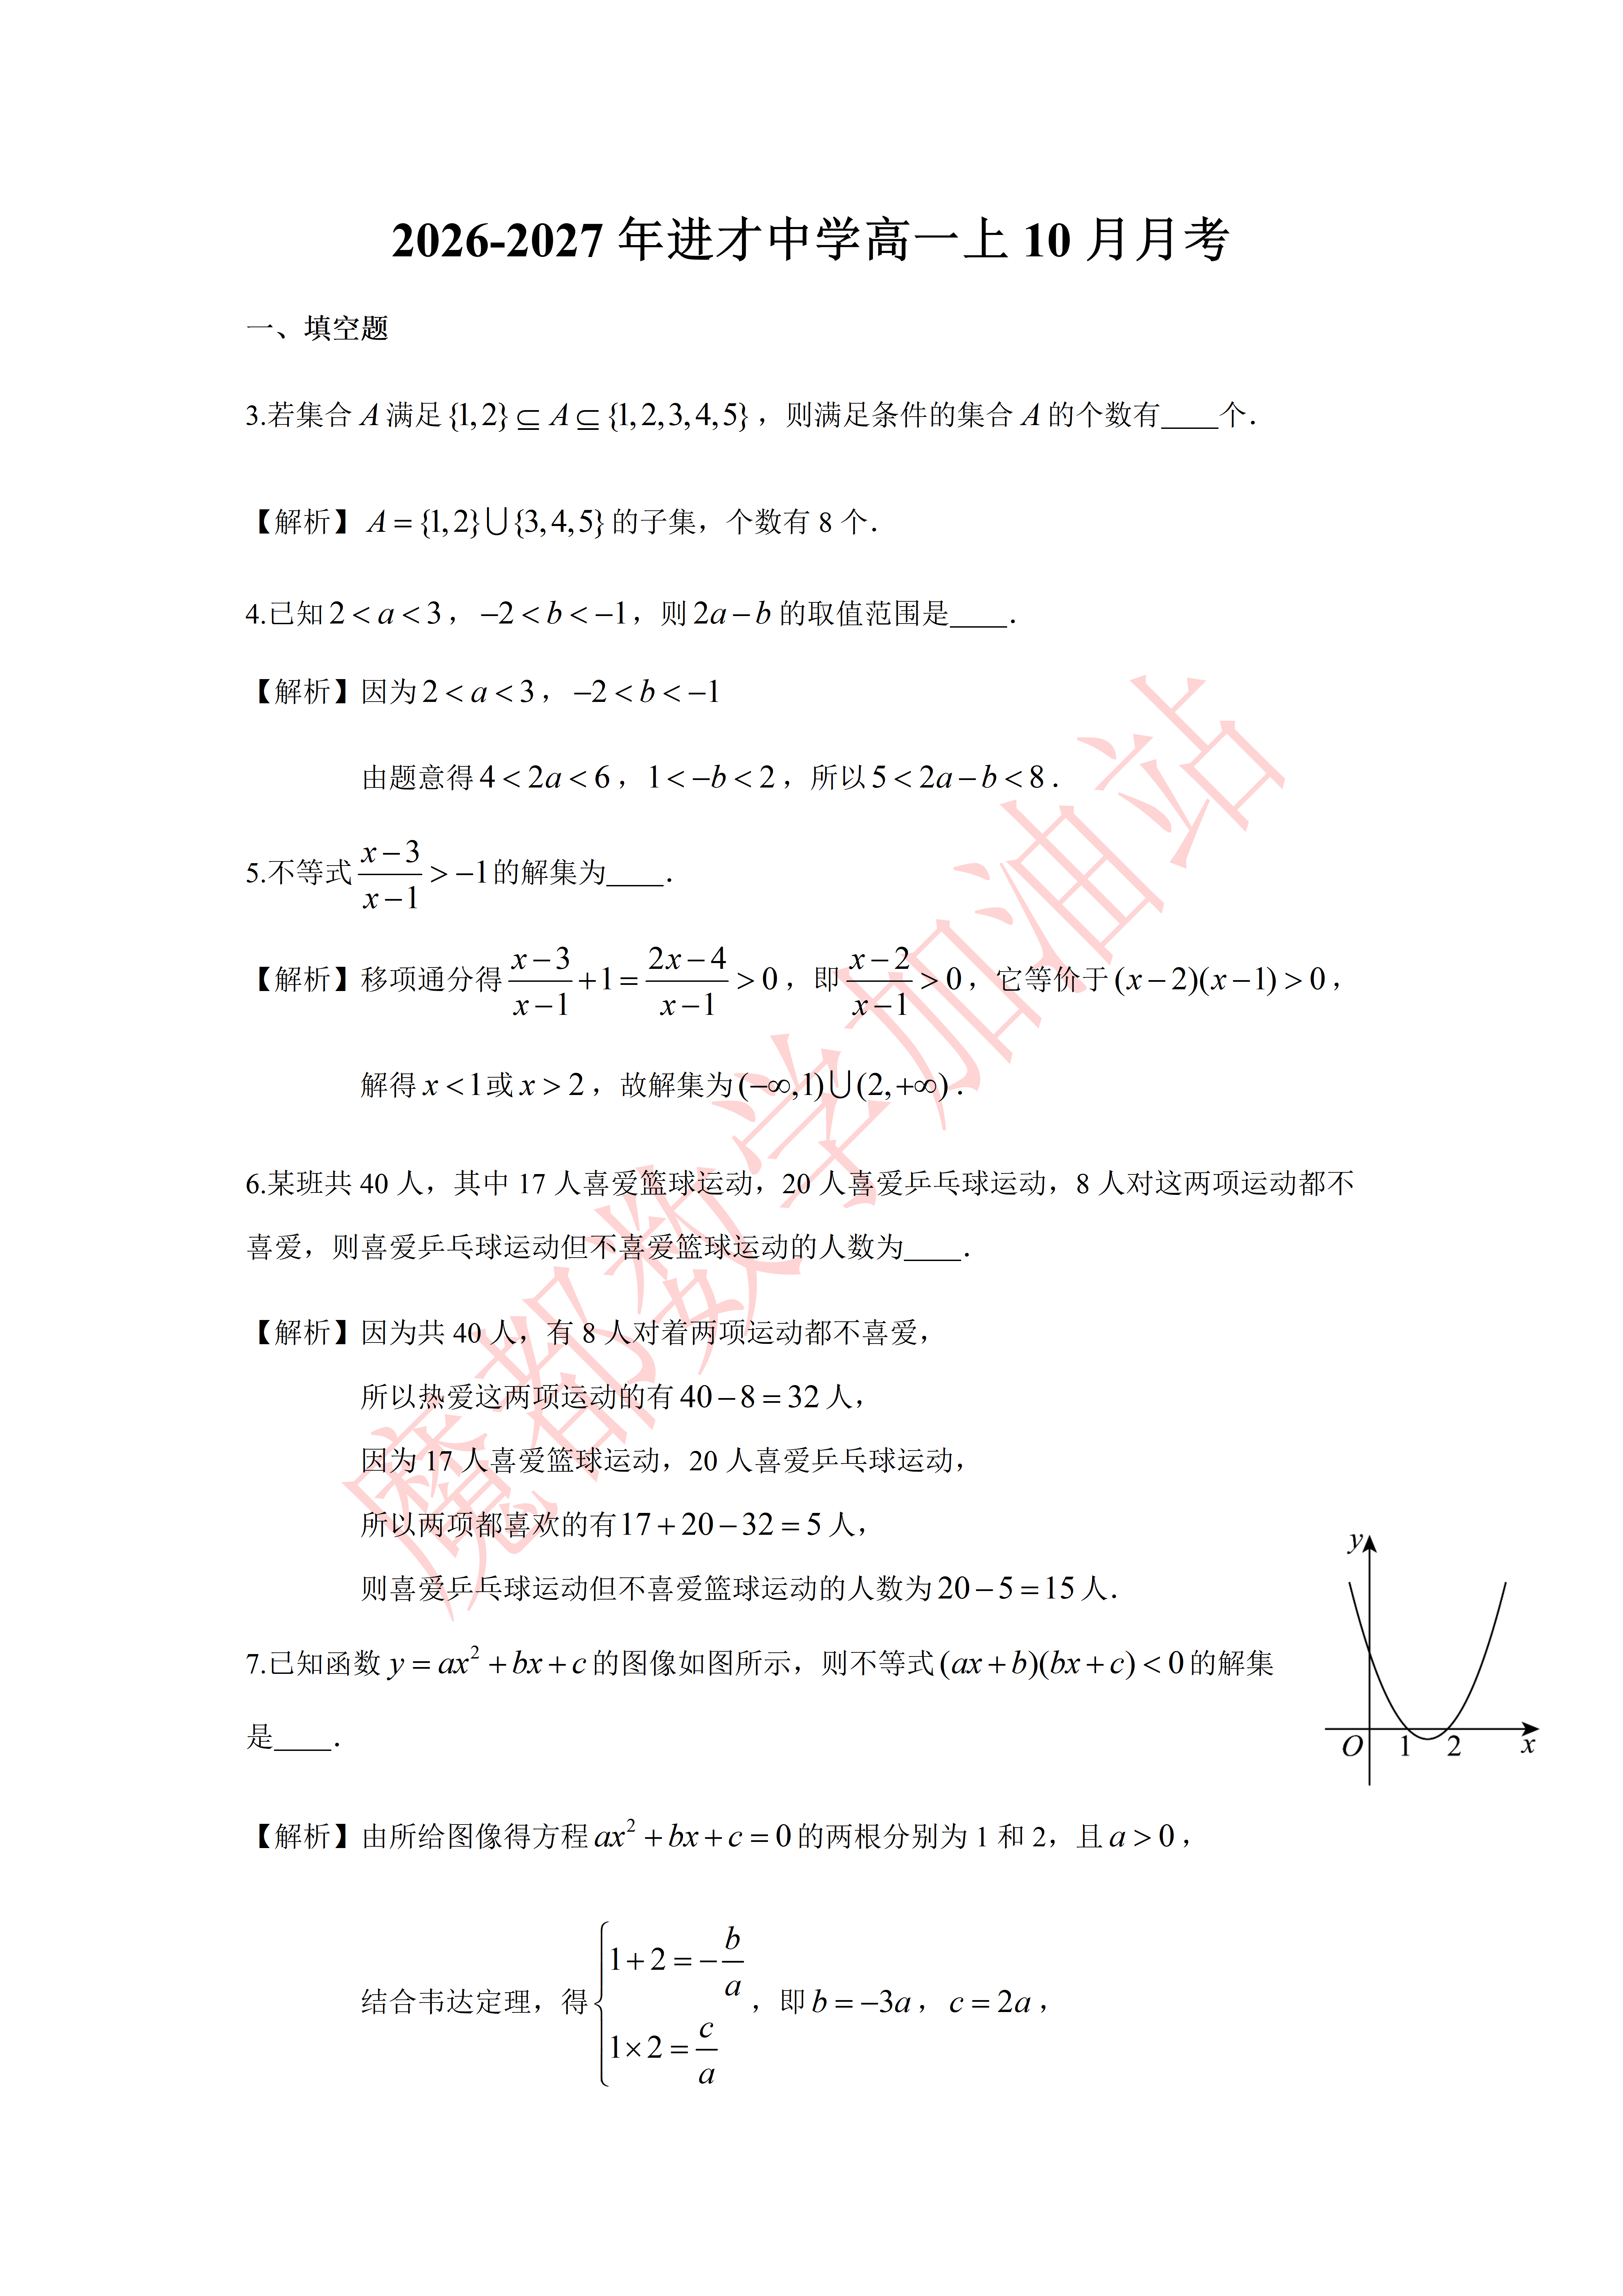
\includegraphics[width=.22\linewidth,trim=3879bp 1490bp 238bp 4492bp,clip]{../原图/高一60_进才中学_10月月考/01.png}
\end{center}

\ifanswer
\solbegin
\step{由所给图像得方程 $ax^2+bx+c=0$ 的两根分别为 1 和 2，且 $a>0$，}
\step{结合韦达定理，得 $\begin{cases}1+2=-\dfrac ba\\ 1\times2=\dfrac ca\end{cases}$，即 $b=-3a$，$c=2a$，}
\step{所以不等式 $(ax+b)(bx+c)<0$ 即 $(ax-3a)(-3ax+2a)<0$，}
\step{化简得 $(x-3)(3x-2)>0$，解得 $x<\dfrac23$ 或 $x>3$，}
\step{所以不等式 $(ax+b)(bx+c)<0$ 的解集是 $(-\infty,\dfrac23)\cup(3,+\infty)$.}
\solend
\fi

\item 已知集合 $A=\{x\mid ax=6\}$，满足 $A\subseteq\Z$，则整数 $a$ 的所有可能取值有\blankline[4.4em]个.

\ifanswer
\solbegin
\step{当 $a=0$ 时，$A=\varnothing$，而 $\varnothing\subseteq\Z$，满足题意，}
\step{当 $a\neq0$ 时，$A=\left\{\dfrac6a\right\}$，要使 $A\subseteq\Z$，则 $\dfrac6a\in\Z$，所以 $a=\pm1,\pm2,\pm3,\pm6$，}
\step{综上，整数 $a$ 的可能取值为 0，$\pm1$，$\pm2$，$\pm3$，$\pm6$，共 9 个.}
\solend
\fi

\item 设关于 $x$ 的方程 $x^2+kx+n=0$ 有两个不同实根 $x_1$、$x_2$，且 $\dfrac1{x_1}+\dfrac1{x_2}=2$，则实数 $n$ 的取值范围是\blankline[4.4em].

\ifanswer
\solbegin
\step{由于方程 $x^2+kx+n=0$ 有两个不同实根 $x_1$、$x_2$，}
\step{因此 $\Delta=k^2-4n>0$，$x_1+x_2=-k$，$x_1x_2=n$，}
\step{由 $\dfrac1{x_1}+\dfrac1{x_2}=\dfrac{x_1+x_2}{x_1x_2}=\dfrac{-k}{n}=2$，得 $k=-2n$，}
\step{因此 $\Delta=k^2-4n=4n^2-4n>0$，解得 $n<0$ 或 $n>1$，}
\step{则实数 $n$ 的取值范围是 $(-\infty,0)\cup(1,+\infty)$.}
\solend
\fi

\item 某船从甲地沿河顺流航行 $75\mathrm{km}$，到达乙码头，停留 $30\mathrm{min}$ 后再逆流航行 $126\mathrm{km}$ 到达丙地，若水流速度为 $4\mathrm{km/h}$，且该船要在 $5\mathrm{h}$ 内完成航行任务，那么船的速度至少达到\blankline[4.4em]$\mathrm{km/h}$.

\ifanswer
\solbegin
\step{设该轮船在静水中的速度是 $x$ 千米/小时，水流速度是 4 千米/小时，}
\step{由题意得 $\dfrac{75}{4+x}+0.5+\dfrac{126}{x-4}\leqslant5$，即 $9x^2-402x-552\geqslant0$，解得 $x\geqslant46$，}
\step{答：该船的速度至少是 46 千米/小时.}
\solend
\fi

\item 设实数 $a,b,c$ 满足 $a^2+b^2\leqslant c<1$，则 $a+\dfrac12b+c$ 的最小值为\blankline[4.4em].

\ifanswer
\solbegin
\step{因为 $c\geqslant a^2+b^2$，}
\step{所以 $a+\dfrac12b+c\geqslant a+\dfrac12b+a^2+b^2=\left(a+\dfrac12\right)^2+\left(b+\dfrac14\right)^2-\dfrac5{16}\geqslant-\dfrac5{16}$，}
\step{当 $a=-\dfrac12,b=-\dfrac14,c=a^2+b^2=\dfrac5{16}$（此时 $c<1$ 成立）时取到等号，}
\step{故最小值为 $-\dfrac5{16}$.}
\solend
\fi

\item 已知集合 $A=\{x\in\N^*\mid1\leqslant x\leqslant2026\}$. 设集合 $B=\{b_1,b_2,b_3,\cdots,b_n\}$ 满足 $B\subseteq A$，且对任意的 $b_i$、$b_j$、$b_k\in B(i$、$j$、$k\in\{1,2,3,\cdots,n\})$，存在 $m\in\N^*$，使得 $b_i+b_j+b_k=39m$，则 $n$ 的最大值为\blankline[4.4em].

\ifanswer
\solbegin
\step{因为 $39=1\times39=3\times13$，所以 $n$ 的最大值大于 3，}
\step{若对任意的 $b_i$、$b_j$、$b_k\in B$，存在 $m\in\N^*$，使得 $b_i+b_j+b_k=39m$，}
\step{则集合 $B$ 的元素除以 39 的余数均为 0 或均为 13 或均为 26，}
\step{即 $B=\{39,78,\cdots,39n\}$ 或 $B=\{13,52,\cdots,39n-26\}$}
\step{或 $B=\{26,65,\cdots,39n-13\}$，}
\step{若 $B=\{39,78,\cdots,39n\}$，则 $39n\leqslant2026$，}
\step{解得 $n\leqslant\dfrac{2026}{39}\in(51,52)$，此时 $n$ 的最大值为 51；}
\step{若 $B=\{13,52,\cdots,39n-26\}$，则 $39n-26\leqslant2026$，}
\step{解得 $n\leqslant\dfrac{684}{13}\in(52,53)$，此时 $n$ 的最大值为 52；}
\step{若 $B=\{26,65,\cdots,39n-13\}$，则 $39n-13\leqslant2026$，}
\step{解得 $n\leqslant\dfrac{2039}{39}\in(52,53)$，此时 $n$ 的最大值为 52；}
\step{综上，$n$ 的最大值为 52.}
\solend
\fi

\end{enumerate}

\bigsec{二、选择题}

\begin{enumerate}
\setcounter{enumi}{12}

% 第 13 题原卷无【答案】/【解析】段，答案“B”直接印在题干括号内，
% 按 高一53 第 13 题的成例括号留空、答案另提为 \ans{}（见文件头）
\item 已知 $a$、$b\in\R$，则“$|a|>|b|$”是“$a>|b|$”的\mbox{（\quad）}

\keepwithprev
A. 充分不必要条件\qquad B. 必要不充分条件

C. 充要条件\qquad D. 既不充分也不必要条件

\ifanswer
\ans{$B$}
\fi

\item 如果关于 $x$ 的一元二次方程 $x^2+2mx+(m+2)=0$ 有一正根一负根，那么 $m$ 的取值范围为\mbox{（\quad）}

\keepwithprev
A. $(-2,-1)$\qquad B. $(-1,2)$

C. $(-\infty,-1)\cup(2,+\infty)$\qquad D. $(-\infty,-2)$

\ifanswer
\solbegin
\step{设两根为 $x_1,x_2$，方程有一正根一负根，则 $\begin{cases}x_1x_2=m+2<0\\ \Delta=4m^2-4(m+2)>0\end{cases}$，}
\step{解得 $m<-2$，故选 $D$.}
\solend
\fi

\item 若不等式 $|3x-a|\leqslant x+2$ 的解集包含集合 $[0,1]$，则实数 $a$ 的取值范围为\mbox{（\quad）}

\keepwithprev
A. $[0,2]$\qquad B. $[0,1]$

C. $[1,2]$\qquad D. $(1,2)$

\ifanswer
\solbegin
% 原卷“法一：”“法二：”排红色加粗（全卷唯一红字），本稿按全稿子题标号样式排 \stepm
% （详见文件头“与原卷的排版差异”⑦）
\stepm{法一：}{不等式 $|3x-a|\leqslant x+2$ 化为 $2x-2\leqslant a\leqslant4x+2$，}
% 原卷此句缺动词（疑漏“对”字），照录未改（见文件头“原卷存疑”④）
\step{$[0,1]$ 使 $2x-2\leqslant a\leqslant4x+2$ 成立，则 $0\leqslant a\leqslant2$，故选 $A$.}
\stepm{法二：}{将两边平方整理得 $8x^2-(6a+4)x+a^2-4\leqslant0$ 对 $[0,1]$ 恒成立，}
\step{则有 $\begin{cases}a^2-4\leqslant0\\ a^2-6a\leqslant0\end{cases}$，解得 $0\leqslant a\leqslant2$，故选 $A$.}
\solend
\fi

\item 数学组 Y 老师在白纸上写下以下四个命题：

①这四个命题中至少有一个是真的；②这四个命题中至少有两个是真的；

③这四个命题中至少有两个是假的；④这四个命题中至少有一个是假的；

每个命题非真即假. 问 Y 老师在纸上写的假命题有几个？\mbox{（\quad）}

\keepwithprev
A. 0\qquad B. 1

C. 2\qquad D. 3

\ifanswer
\solbegin
\step{设四个命题中真命题的个数为 $t$，则①真 $\iff t\geqslant1$，②真 $\iff t\geqslant2$，}
\step{③真 $\iff t\leqslant2$，④真 $\iff t\leqslant3$.}
\step{逐一检验：$t=0$ 时③④为真，应为 $t=2$，矛盾；}
\step{$t=1$ 时①③④为真，应为 $t=3$，矛盾；}
\step{$t=2$ 时四个命题全为真，应为 $t=4$，矛盾；}
\step{$t=3$ 时①②④为真、③为假，恰有 3 个真命题，符合；}
\step{$t=4$ 时①②为真，应为 $t=2$，矛盾.}
\step{所以恰有 1 个假命题，故选 $B$.}
\solend
\fi

\end{enumerate}

\bigsec{三、解答题}

\begin{enumerate}
\setcounter{enumi}{16}

\item 已知：$x\in\R$，$a=x^2-1$，$b=4x+5$. 求证：$a$、$b$ 中至少有一个大于等于 0.

\ifanswer
\solbegin
\step{假设 $a$、$b$ 都小于 0，即 $a<0$，$b<0$，则 $a+b<0$.}
\step{又 $a+b=x^2-1+4x+5=x^2+4x+4=(x+2)^2\geqslant0$，}
\step{这与假设所得 $a+b<0$ 矛盾，故假设不成立，}
\step{所以 $a$、$b$ 中至少有一个大于等于 0.}
\solend
\fi

\ansspace[6]

% 原卷 A、B 两个集合定义之间排半角逗号“,”（5 倍放大核，右侧字距 19px，与全卷全角“，”的 65—79px 字距判然有别）；
% 本稿原误抄为全角“，”——已照录原卷半角（见文件头“与原卷的排版差异”⑤）
\item 已知集合 $A=\{x\mid4\leqslant x\leqslant12\}$,$B=\{x\mid a\leqslant x\leqslant2a+1\}$.

（1）若 $a=2$，求 $\overline A\cap B$；

（2）已知 $A\cup B=A$，求实数 $a$ 的取值范围.

\ifanswer
\solbegin
\stepm{(1)}{当 $a=2$ 时，$B=\{x\mid2\leqslant x\leqslant5\}$，}
\step{而 $A=\{x\mid4\leqslant x\leqslant12\}$，则 $\overline A=(-\infty,4)\cup(12,+\infty)$，所以 $\overline A\cap B=[2,4)$.}
\stepm{(2)}{$A\cup B=A$ 即 $B\subseteq A$.}
\stepm{①}{当 $B=\varnothing$ 时，$a>2a+1$，即 $a<-1$，符合；}
\stepm{②}{当 $B\neq\varnothing$ 时，需 $a\leqslant2a+1$ 且 $a\geqslant4$ 且 $2a+1\leqslant12$，即 $4\leqslant a\leqslant\dfrac{11}2$.}
\step{综上，$a$ 的取值范围是 $(-\infty,-1)\cup\left[4,\dfrac{11}2\right]$.}
\solend
\fi

\ansspace[8]

\item （1）若关于 $x$ 的不等式 $ax^2-3x+2<0$ 的解集不是空集，求实数 $a$ 的取值范围；

（2）求关于 $x$ 的不等式 $ax^2-3x+2>ax-1$ 的解集.

\ifanswer
\solbegin
\stepm{(1)}{若 $a>0$，关于 $x$ 的不等式 $ax^2-3x+2<0$ 的解集不空，}
\step{所以一元二次方程 $ax^2-3x+2=0$ 的判别式大于零，}
\step{即 $(-3)^2-8a>0\Rightarrow a<\dfrac98$，结合 $a>0$ 得 $0<a<\dfrac98$；}
\step{若 $a\leqslant0$，则关于 $x$ 的不等式 $ax^2-3x+2<0$ 的解集不是空集；}
\step{综上，实数 $a$ 的取值范围是 $\left(-\infty,\dfrac98\right)$.}
\stepm{(2)}{$ax^2-3x+2>ax-1\Rightarrow ax^2-(a+3)x+3>0\Rightarrow(ax-3)(x-1)>0$，}
\step{当 $a=0$ 时，不等式为 $x-1<0$，不等式的解集为 $\{x\mid x<1\}$；}
\step{当 $a<0$ 时，不等式化为 $\left(x-\dfrac3a\right)(x-1)<0$，}
\step{不等式的解集为 $\left\{x\mid\dfrac3a<x<1\right\}$，}
\step{当 $a>0$ 时，方程 $ax^2-3x+2=ax-1$ 的两个根分别为：$\dfrac3a,1$.}
\step{当 $a=3$ 时，两根相等，故不等式的解集为 $\{x\mid x\neq1\}$；}
\step{当 $a>3$ 时，$\dfrac3a<1$，不等式的解集为 $\left\{x\mid x<\dfrac3a\right.$ 或 $\left.x>1\right\}$；}
\step{当 $0<a<3$ 时，$\dfrac3a>1$，不等式的解集为 $\left\{x\mid x<1\right.$ 或 $\left.x>\dfrac3a\right\}$；}
\step{综上所述，当 $a<0$ 时，不等式的解集为 $\left\{x\mid\dfrac3a<x<1\right\}$，}
\step{当 $a=0$ 时，不等式的解集为 $\{x\mid x<1\}$，}
\step{当 $0<a<3$ 时，不等式的解集为 $\left\{x\mid x<1\right.$ 或 $\left.x>\dfrac3a\right\}$，}
\step{当 $a=3$ 时，不等式的解集为 $\{x\mid x\neq1\}$，}
\step{当 $a>3$ 时，不等式的解集为 $\left\{x\mid x<\dfrac3a\right.$ 或 $\left.x>1\right\}$.}
\solend
\fi

\ansspace[8]

\item 设命题 $p$：对任意 $x\in\R$，使得不等式 $mx^2-mx+2>0$ 恒成立；命题 $q$：存在 $0\leqslant x\leqslant3$，不等式 $2x-2\geqslant|m|$ 成立.

（1）若 $p$ 为真命题，求实数 $m$ 的取值范围；

（2）若 $p$、$q$ 有且只有一个是真命题，求实数 $m$ 的取值范围.

\ifanswer
\solbegin
\stepm{(1)}{因为 $p:\forall x\in\R$，$mx^2-mx+2>0$ 为真命题，}
\step{所以当 $m=0$ 时，不等式为 $2>0$，在 $\R$ 上恒成立，符合题意；}
\step{当 $m\neq0$ 时，$\begin{cases}m>0\\ \Delta=m^2-8m<0\end{cases}$，解得 $0<m<8$.}
\step{综上，实数 $m$ 的取值范围为 $[0,8)$.}
\stepm{(2)}{若 $q$ 为真命题，即 $q:\exists0\leqslant x\leqslant3$，$2x-2\geqslant|m|$，}
\step{则对于 $0\leqslant x\leqslant3$，$(2x-2)_{max}\geqslant|m|$.}
\step{由于 $0\leqslant x\leqslant3$，$2x-2\in[-2,4]$，所以 $|m|\leqslant4$，解得 $-4\leqslant m\leqslant4$，}
\step{又因为 $p$、$q$ 有且只有一个是真命题，}
\step{所以当 $p$ 真 $q$ 假时，$\begin{cases}0\leqslant m<8\\ m<-4\text{或}m>4\end{cases}$，解得 $4<m<8$；}
\step{当 $p$ 假 $q$ 真时，$\begin{cases}m<0\text{或}m\geqslant8\\ -4\leqslant m\leqslant4\end{cases}$，解得 $-4\leqslant m<0$；}
\step{综上，实数 $m$ 的取值范围为 $[-4,0)\cup(4,8)$.}
\solend
\fi

\ansspace[10]

\item 已知集合 $A=\{a_1,a_2,\cdots,a_k\}(k\geqslant2)$. 其中 $a_i\in\N^*(i=1,2,\cdots,k)$. 若对于任意的 $a\in A$，总有 $\dfrac1a\notin A$，则称集合 $A$ 具有性质 $P$. 由 $A$ 中的元素构成两个相应的集合：$S=\{(a,b)\mid a\in A,b\in A,ab\in A\}$，$T=\left\{(a,b)\mid a\in A,b\in A,\dfrac ab\in A\right\}$，其中 $(a,b)$ 是有序数对，集合 $S$ 和 $T$ 中的元素个数分别为 $m$ 和 $n$.

（1）检验集合 $\{2,3,6\}$ 与 $\{1,2,4\}$ 是否具有性质 $P$，并对其中具有性质 $P$ 的集合，写出相应的集合 $S$ 和 $T$；

（2）对任何具有性质 $P$ 的集合 $A$，$n$ 的最大值为多少？（直接写出答案，无需说明理由）；

% 原卷题干的小问编号跳号：印作 (1)(2)(4)，本稿照录 (4)、未改成 (3)（见文件头“原卷存疑”①）
（4）判断 $m$ 和 $n$ 的大小关系，并证明你的结论.

\ifanswer
\solbegin
\stepm{(1)}{因为 $\dfrac12\in\{1,2,4\}$，所以 $\{1,2,4\}$ 不具有性质 $P$；}
\step{因为 $\dfrac12\notin\{2,3,6\}$，$\dfrac13\notin\{2,3,6\}$，$\dfrac16\notin\{2,3,6\}$，所以 $\{2,3,6\}$ 具有性质 $P$.}
\step{$S=\{(2,3),(3,2)\}$，$T=\{(6,2),(6,3)\}$；}
\stepm{(2)}{因为对于任意的 $a\in A$，总有 $\dfrac1a\notin A$，所以 $1\notin A$，}
% 原卷此处印作“$\{(a_i,a_i)\}\in T$”，与上一句“$1\notin A$”及下文“最多为 $C_k^2$”的推理
% 均不自洽（应为“$\notin$”），已 8 倍放大确认无斜线；照录未改（见文件头“原卷存疑”③）
\step{从而 $\{(a_i,a_i)\}\in T(i=1,2,\cdots,k)$.}
\step{因为 $a\in A,b\in A,\dfrac ab\in A$，所以当 $i\neq j$ 时，}
\step{$(a_i,a_j)\in T$ 和 $(a_j,a_i)\in T(i,j=1,2,\cdots,k)$ 至多有一个成立，}
\step{所以集合 $T$ 中的元素个数最多为 $C_k^2=\dfrac{k(k-1)}2$，即 $n\leqslant\dfrac{k(k-1)}2$.}
% 原卷【解析】把第 (4) 问标作“(3)”（与题干跳号相应），本稿照录未改（见文件头“原卷存疑”①）
\stepm{(3)}{$m=n$，证明如下：}
\step{①设 $(a,b)\in T$，则 $a\in A,b\in A,\dfrac ab\in A$. 设 $c=\dfrac ab$，则 $a=bc$，}
\step{故 $b\in A$，$c\in A$，$bc\in A$，从而 $(b,c)\in S$，}
\step{即对 $\forall(a,b)\in T$，总 $\exists c$ 使 $(b,c)\in S$，从而 $n\leqslant m$.}
\step{②设 $(p,q)\in S$，则 $p\in A$，$q\in A$，$pq\in A$.}
\step{设 $r=pq$，则 $q=\dfrac rp$，故 $r\in A,p\in A,\dfrac rp\in A$，从而 $(r,p)\in T$，}
\step{即对 $\forall(p,q)\in S$，总 $\exists r$ 使 $(r,p)\in T$，从而 $m\leqslant n$.}
\step{由①②得 $m=n$.}
\solend
\fi

\ansspace*[10]

\end{enumerate}

\end{document}
"
% 紧凑版：xelatex "\def\iscompact{1}% 高一60_进才中学_10月月考.tex
%   —— 高一上数学“2026-2027 年进才中学高一上 10 月月考”（讲评版）
% 试卷版：xelatex 高一60_进才中学_10月月考.tex
% 答案版：xelatex "\def\isanswer{1}% 高一60_进才中学_10月月考.tex
%   —— 高一上数学“2026-2027 年进才中学高一上 10 月月考”（讲评版）
% 试卷版：xelatex 高一60_进才中学_10月月考.tex
% 答案版：xelatex "\def\isanswer{1}% 高一60_进才中学_10月月考.tex
%   —— 高一上数学“2026-2027 年进才中学高一上 10 月月考”（讲评版）
% 试卷版：xelatex 高一60_进才中学_10月月考.tex
% 答案版：xelatex "\def\isanswer{1}\input{高一60_进才中学_10月月考.tex}"
% 紧凑版：xelatex "\def\iscompact{1}\input{高一60_进才中学_10月月考.tex}"
%
% 原文链接：https://mp.weixin.qq.com/s/2ZLKB3IONEDhcUAfAAYE2A。
% 公众号“魔都数学加油站”作者破晓于 2026-10-14 22:15 发布。
% 原图 9 张（`原图/高一60_进才中学_10月月考/01..09.png`）：第 1—8 页 4762×6735，
% 第 9 页 2560×3620（同一篇内两档分辨率）。
%
% 卷首标题：照卷面印作“2026--2027 年进才中学高一上 10 月月考”（公众号标题中的“上海市”
% 卷面标题行没有，本稿照卷面），年份区间按全稿惯例排 en dash。原卷只有一行标题、无副标题。
%
% 篇幅与题号：原卷自第 3 题起编号（第 1、2 题不在本卷内）。填空题 3—12（10 题）、
% 选择题 13—16（4 题）、解答题 17—21（5 题），共 19 题。本稿沿用原节与原题号，
% 只改排为全稿统一的大节样式（原卷小节标题为“一、填空题”“二、选择题”“三、解答题”）。
%
% 讲评版：原卷每题下直接印【答案】或【解析】。**只印【解析】的 18 题**，本稿按全稿口径
% 收进答案版、不另提 \ans{}——第 14、15、16 题的结论写在解析末句（“故选 D／A／B”），
% 亦照录在解析内。**第 13 题原卷没有任何【答案】/【解析】段**，答案“B”直接印在题干括号内
% （“（ B ）”），本稿按 高一53 第 13 题的成例把括号留空、答案另提为 \ans{$B$}（见下）。
%
% 副标题：原卷未印副标题。本稿按“知识模块”口径标作“集合与常用逻辑用语、不等式”：
% 19 题中集合与常用逻辑用语 10 题（第 3、6、8、12、13、16、17、18、20、21 题，
% 含子集计数、韦恩图容斥、集合运算、命题与充要条件、反证法、新定义），
% 不等式 9 题（含不等式性质、分式不等式、二次函数与解集、韦达定理与判别式、
% 不等式应用、最值、根的分布、绝对值不等式恒成立、含参二次不等式：第 4、5、7、9、10、
% 11、14、15、19 题），两类均远超三分之一，故并标。口径同 高一46、高一47、高一48、
% 高一51—高一59。
%
% 与原卷的排版差异：
%   ① 原卷每题下直接印【答案】/【解析】，本稿按全稿惯例将答案与解析置于答案版，试卷版保持干净；
%   ② 原卷未印副标题，本稿按“知识模块”口径补出；
%   ③ 原卷填空横线约两个字宽，本稿按全稿惯例统一排 \blankline[4.4em]；
%   ④ 原卷实数集排斜体 $R$（第 13、17、20 题）、正整数集排 $N^*$（第 12、21 题）、
%      整数集排粗体 $\mathbf{Z}$（第 8 题），本稿按全稿惯例改用 $\R$、$\N^*$、$\Z$；
%      空集记号统一为 \varnothing；
%   ⑤ 原卷在数学式内多处用半角逗号（如 $x_1,x_2$、$a,b\in R$，以及第 18 题题干
%      $A=\{x\mid4\leqslant x\leqslant12\}$,$B=\{x\mid a\leqslant x\leqslant2a+1\}$ 之间的逗号），
%      均照录未强改（第 18 题题干那一处本稿首轮曾误作全角“，”，第二轮已订正）；
%      句末句点按全稿惯例排西文句点；
%   ⑥ 第 13 题印在题干括号内的答案“B”移入 \ans{}，见上；
%   ⑦ 第 15 题【解析】的“法一：”“法二：”标号原卷排**红色加粗**（全卷唯一的红字，2 处），
%      本稿按全稿子题标号样式排 \stepm{法一：}{…}、\stepm{法二：}{…}（加粗着色、不改黑色
%      基调），冒号照原卷排全角；
%   ⑧ 第 7 题的图像原卷排在题干右侧（与题干第 1 行同高），本稿居中排在题干之后；
%      图自原图第 01 页裁切（trim），不另存图片文件；
%   ⑨ 原卷第 10 题的长度与速度单位原卷排斜体（$75km$、$4km/h$ 等），本稿按全稿惯例
%      改排正体 $\mathrm{km}$、$\mathrm{km/h}$（同 高一56 第 13 题）；每道解答题原卷未留
%      作答空白，本稿按全稿惯例加 \ansspace。
%
% 原卷存疑（照录未改，见源码中该处上方注释）：
%   ① 第 21 题题干的小问编号**跳号**：印作 (1)(2)(4)，而紧随其后的【解析】按 (1)(2)(3) 写
%      —— 题干第 (4) 问实为第 (3) 问。本稿题干照录 (1)(2)(4)、解析照录 (3)，未改
%      （与 高一22 第 16 题“解析误标 (2)”同一处理）。
%   ② 第 6 题【解析】“有 8 人**对着**两项运动都不喜爱”，“对着”疑为“对这”之误，照录未改。
%   ③ 第 21(2) 题【解析】首行“所以 $1\notin A$，从而 $\{(a_i,a_i)\}\in T(i=1,2,\cdots,k)$”
%      —— 由 $1\notin A$ 应得 $(a_i,a_i)\notin T$（因 $a_i/a_i=1$），与紧随的“$T$ 中元素
%      个数最多为 $C_k^2$”这一推理亦只有“$\notin$”才自洽；原卷此处印作“$\in$”，
%      已 8 倍放大确认无斜线。**照录原卷的 $\in$、未改**。
%   ④ 第 15 题【解析】法一“$[0,1]$ 使 $2x-2\leqslant a\leqslant4x+2$ 成立”一句缺动词
%      （疑漏“对”字），照录未改。
%
\documentclass[a4paper,11pt]{article}
\usepackage{common}

\begin{document}

\examtitlest[3]{2026--2027 年进才中学高一上 10 月月考}{集合与常用逻辑用语、不等式}

\bigsec{一、填空题}

\begin{enumerate}
\setcounter{enumi}{2}

\item 若集合 $A$ 满足 $\{1,2\}\subseteq A\subseteq\{1,2,3,4,5\}$，则满足条件的集合 $A$ 的个数有\blankline[4.4em]个.

\ifanswer
\solbegin
\step{$A=\{1,2\}\cup\{3,4,5\}$ 的子集，个数有 8 个.}
\solend
\fi

\item 已知 $2<a<3$，$-2<b<-1$，则 $2a-b$ 的取值范围是\blankline[4.4em].

\ifanswer
\solbegin
\step{因为 $2<a<3$，$-2<b<-1$，}
\step{由题意得 $4<2a<6$，$1<-b<2$，所以 $5<2a-b<8$.}
\solend
\fi

\item 不等式 $\dfrac{x-3}{x-1}>-1$ 的解集为\blankline[4.4em].

\ifanswer
\solbegin
\step{移项通分得 $\dfrac{x-3}{x-1}+1=\dfrac{2x-4}{x-1}>0$，即 $\dfrac{x-2}{x-1}>0$，它等价于 $(x-2)(x-1)>0$，}
\step{解得 $x<1$ 或 $x>2$，故解集为 $(-\infty,1)\cup(2,+\infty)$.}
\solend
\fi

\item 某班共 40 人，其中 17 人喜爱篮球运动，20 人喜爱乒乓球运动，8 人对这两项运动都不喜爱，则喜爱乒乓球运动但不喜爱篮球运动的人数为\blankline[4.4em].

\ifanswer
\solbegin
% 原卷作“对着两项运动都不喜爱”（疑为“对这”之误），照录未改（见文件头“原卷存疑”②）
\step{因为共 40 人，有 8 人对着两项运动都不喜爱，}
\step{所以热爱这两项运动的有 $40-8=32$ 人，}
\step{因为 17 人喜爱篮球运动，20 人喜爱乒乓球运动，}
\step{所以两项都喜欢的有 $17+20-32=5$ 人，}
\step{则喜爱乒乓球运动但不喜爱篮球运动的人数为 $20-5=15$ 人.}
\solend
\fi

\item 已知函数 $y=ax^2+bx+c$ 的图像如图所示，则不等式 $(ax+b)(bx+c)<0$ 的解集是\blankline[4.4em].

% 原图第 01 页题干右侧的图像直接裁取。裁框取图外框 x 3887–4516、y 4500–5237
% （四周各留约 8px），trim=左 3879bp／下 1490bp／右 238bp／上 4492bp
% （页宽 4762、页高 6735）。
\begin{center}
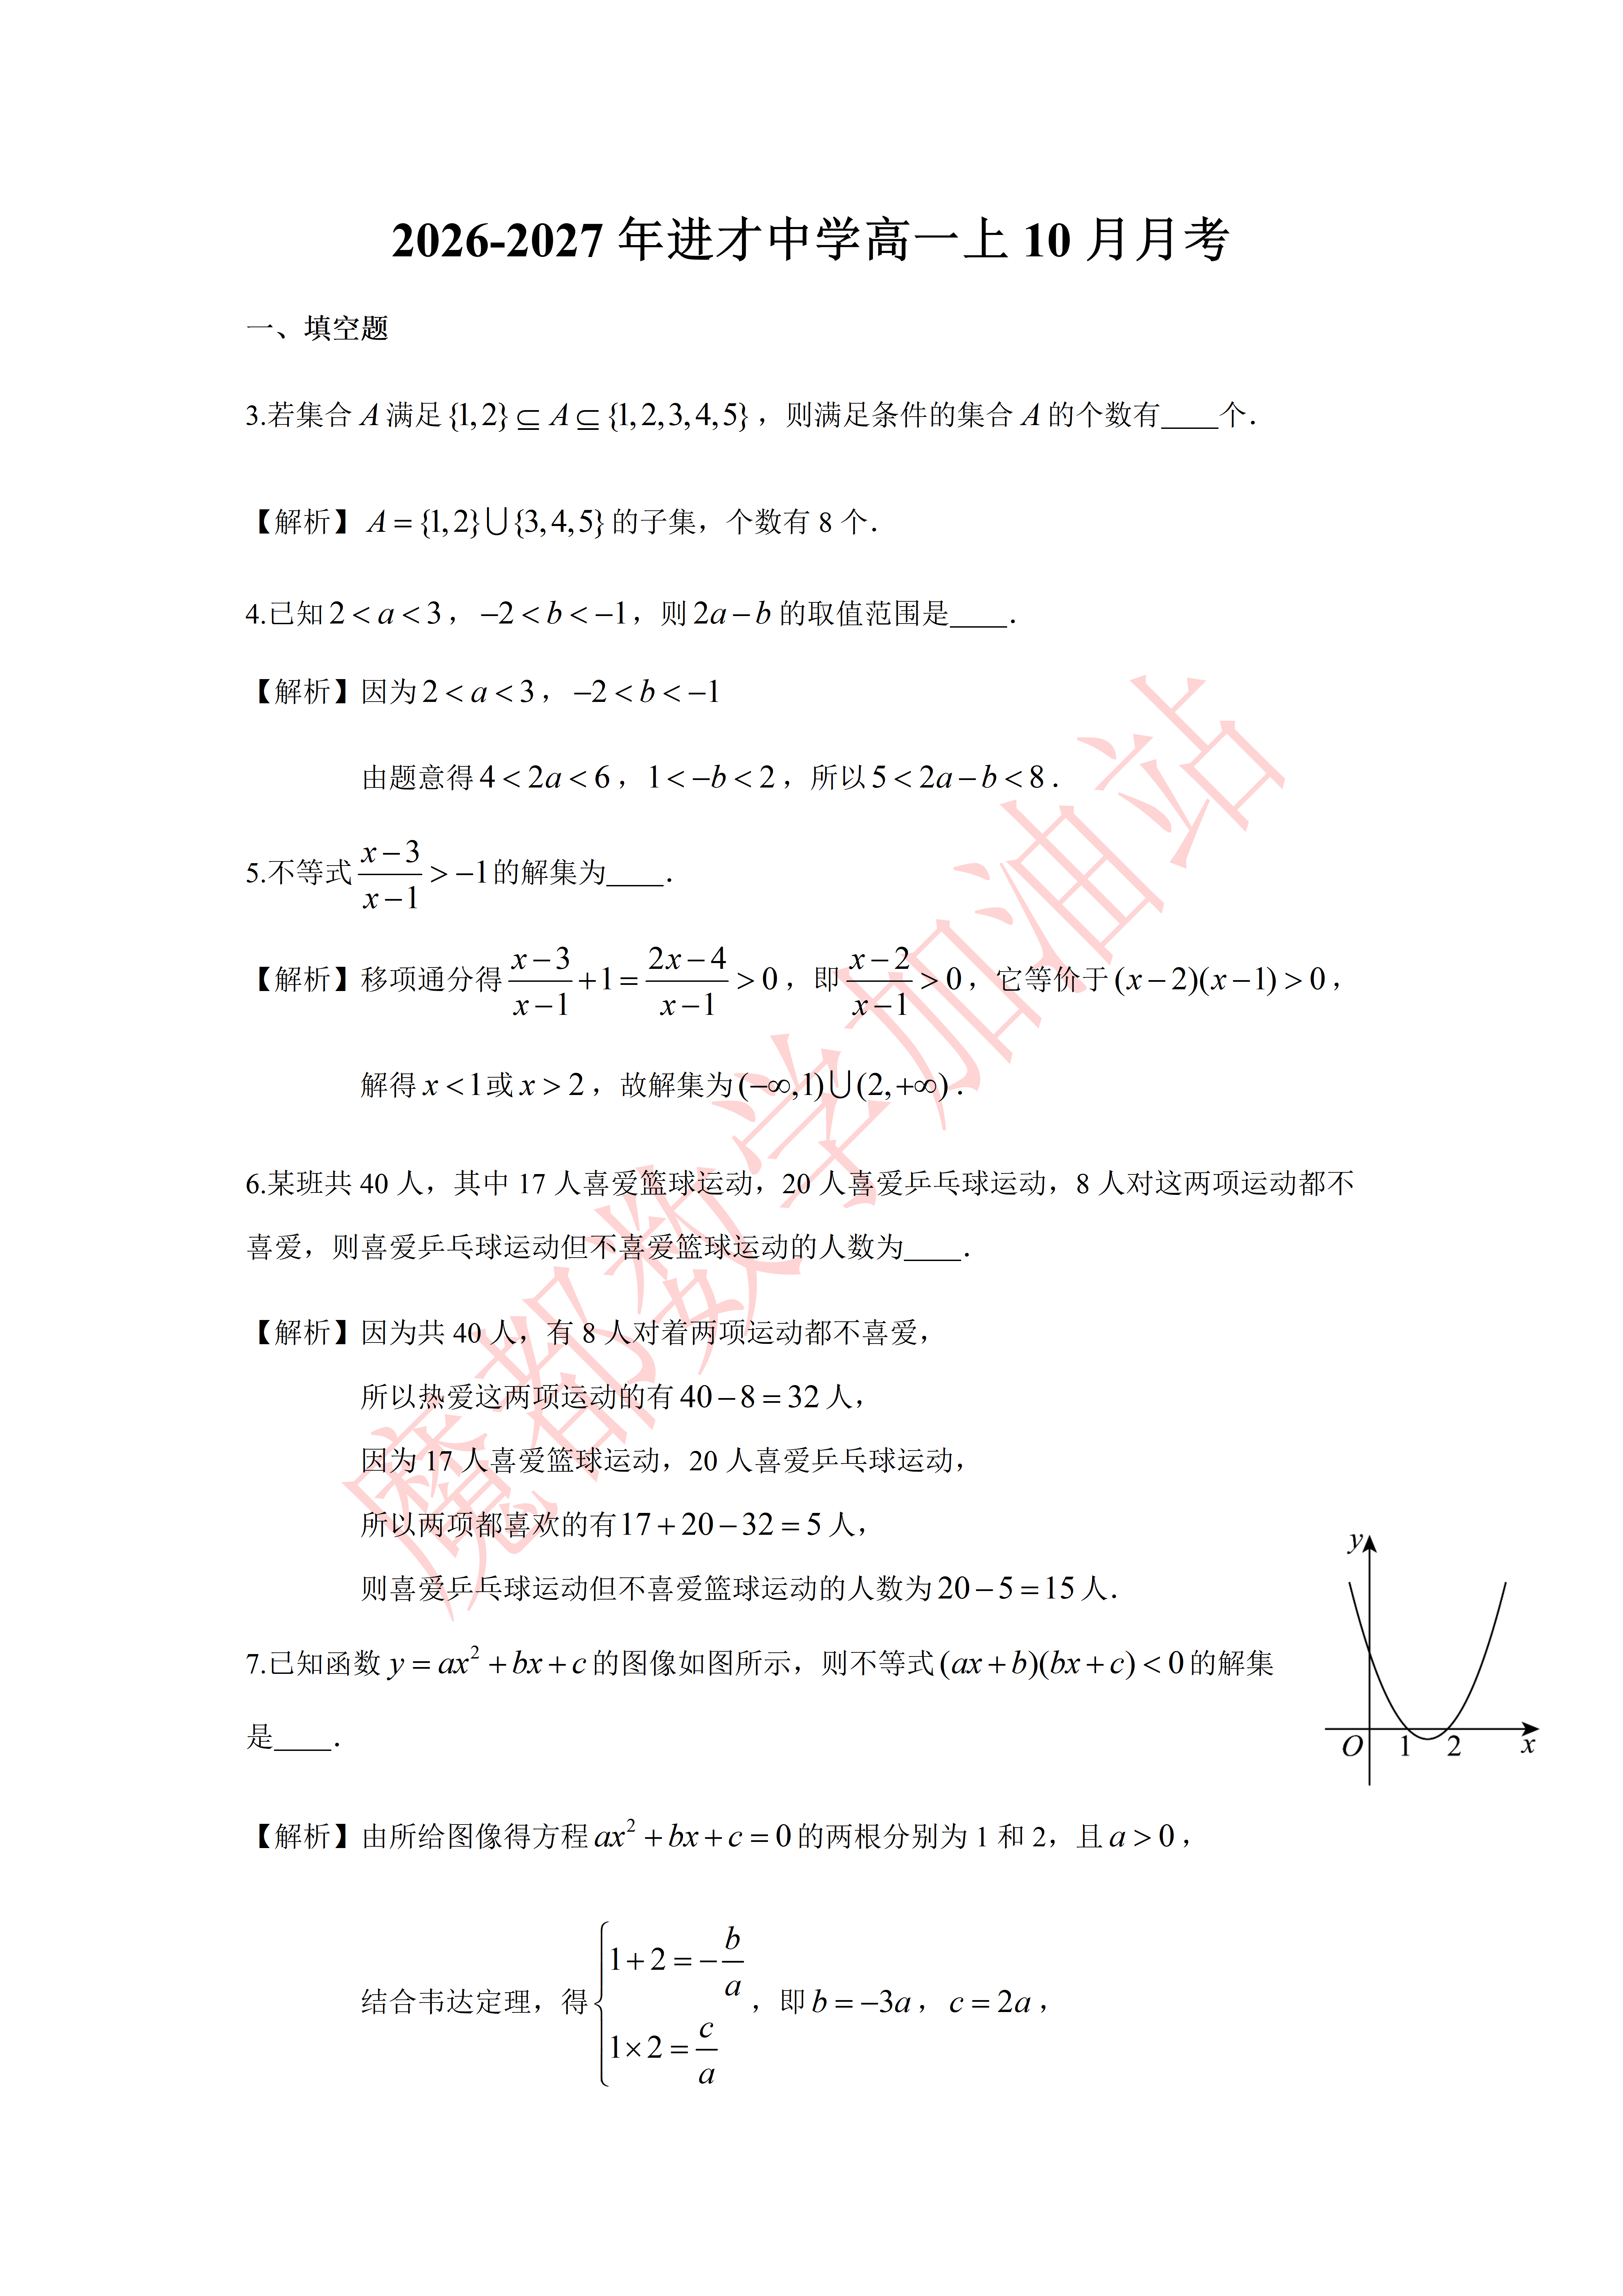
\includegraphics[width=.22\linewidth,trim=3879bp 1490bp 238bp 4492bp,clip]{../原图/高一60_进才中学_10月月考/01.png}
\end{center}

\ifanswer
\solbegin
\step{由所给图像得方程 $ax^2+bx+c=0$ 的两根分别为 1 和 2，且 $a>0$，}
\step{结合韦达定理，得 $\begin{cases}1+2=-\dfrac ba\\ 1\times2=\dfrac ca\end{cases}$，即 $b=-3a$，$c=2a$，}
\step{所以不等式 $(ax+b)(bx+c)<0$ 即 $(ax-3a)(-3ax+2a)<0$，}
\step{化简得 $(x-3)(3x-2)>0$，解得 $x<\dfrac23$ 或 $x>3$，}
\step{所以不等式 $(ax+b)(bx+c)<0$ 的解集是 $(-\infty,\dfrac23)\cup(3,+\infty)$.}
\solend
\fi

\item 已知集合 $A=\{x\mid ax=6\}$，满足 $A\subseteq\Z$，则整数 $a$ 的所有可能取值有\blankline[4.4em]个.

\ifanswer
\solbegin
\step{当 $a=0$ 时，$A=\varnothing$，而 $\varnothing\subseteq\Z$，满足题意，}
\step{当 $a\neq0$ 时，$A=\left\{\dfrac6a\right\}$，要使 $A\subseteq\Z$，则 $\dfrac6a\in\Z$，所以 $a=\pm1,\pm2,\pm3,\pm6$，}
\step{综上，整数 $a$ 的可能取值为 0，$\pm1$，$\pm2$，$\pm3$，$\pm6$，共 9 个.}
\solend
\fi

\item 设关于 $x$ 的方程 $x^2+kx+n=0$ 有两个不同实根 $x_1$、$x_2$，且 $\dfrac1{x_1}+\dfrac1{x_2}=2$，则实数 $n$ 的取值范围是\blankline[4.4em].

\ifanswer
\solbegin
\step{由于方程 $x^2+kx+n=0$ 有两个不同实根 $x_1$、$x_2$，}
\step{因此 $\Delta=k^2-4n>0$，$x_1+x_2=-k$，$x_1x_2=n$，}
\step{由 $\dfrac1{x_1}+\dfrac1{x_2}=\dfrac{x_1+x_2}{x_1x_2}=\dfrac{-k}{n}=2$，得 $k=-2n$，}
\step{因此 $\Delta=k^2-4n=4n^2-4n>0$，解得 $n<0$ 或 $n>1$，}
\step{则实数 $n$ 的取值范围是 $(-\infty,0)\cup(1,+\infty)$.}
\solend
\fi

\item 某船从甲地沿河顺流航行 $75\mathrm{km}$，到达乙码头，停留 $30\mathrm{min}$ 后再逆流航行 $126\mathrm{km}$ 到达丙地，若水流速度为 $4\mathrm{km/h}$，且该船要在 $5\mathrm{h}$ 内完成航行任务，那么船的速度至少达到\blankline[4.4em]$\mathrm{km/h}$.

\ifanswer
\solbegin
\step{设该轮船在静水中的速度是 $x$ 千米/小时，水流速度是 4 千米/小时，}
\step{由题意得 $\dfrac{75}{4+x}+0.5+\dfrac{126}{x-4}\leqslant5$，即 $9x^2-402x-552\geqslant0$，解得 $x\geqslant46$，}
\step{答：该船的速度至少是 46 千米/小时.}
\solend
\fi

\item 设实数 $a,b,c$ 满足 $a^2+b^2\leqslant c<1$，则 $a+\dfrac12b+c$ 的最小值为\blankline[4.4em].

\ifanswer
\solbegin
\step{因为 $c\geqslant a^2+b^2$，}
\step{所以 $a+\dfrac12b+c\geqslant a+\dfrac12b+a^2+b^2=\left(a+\dfrac12\right)^2+\left(b+\dfrac14\right)^2-\dfrac5{16}\geqslant-\dfrac5{16}$，}
\step{当 $a=-\dfrac12,b=-\dfrac14,c=a^2+b^2=\dfrac5{16}$（此时 $c<1$ 成立）时取到等号，}
\step{故最小值为 $-\dfrac5{16}$.}
\solend
\fi

\item 已知集合 $A=\{x\in\N^*\mid1\leqslant x\leqslant2026\}$. 设集合 $B=\{b_1,b_2,b_3,\cdots,b_n\}$ 满足 $B\subseteq A$，且对任意的 $b_i$、$b_j$、$b_k\in B(i$、$j$、$k\in\{1,2,3,\cdots,n\})$，存在 $m\in\N^*$，使得 $b_i+b_j+b_k=39m$，则 $n$ 的最大值为\blankline[4.4em].

\ifanswer
\solbegin
\step{因为 $39=1\times39=3\times13$，所以 $n$ 的最大值大于 3，}
\step{若对任意的 $b_i$、$b_j$、$b_k\in B$，存在 $m\in\N^*$，使得 $b_i+b_j+b_k=39m$，}
\step{则集合 $B$ 的元素除以 39 的余数均为 0 或均为 13 或均为 26，}
\step{即 $B=\{39,78,\cdots,39n\}$ 或 $B=\{13,52,\cdots,39n-26\}$}
\step{或 $B=\{26,65,\cdots,39n-13\}$，}
\step{若 $B=\{39,78,\cdots,39n\}$，则 $39n\leqslant2026$，}
\step{解得 $n\leqslant\dfrac{2026}{39}\in(51,52)$，此时 $n$ 的最大值为 51；}
\step{若 $B=\{13,52,\cdots,39n-26\}$，则 $39n-26\leqslant2026$，}
\step{解得 $n\leqslant\dfrac{684}{13}\in(52,53)$，此时 $n$ 的最大值为 52；}
\step{若 $B=\{26,65,\cdots,39n-13\}$，则 $39n-13\leqslant2026$，}
\step{解得 $n\leqslant\dfrac{2039}{39}\in(52,53)$，此时 $n$ 的最大值为 52；}
\step{综上，$n$ 的最大值为 52.}
\solend
\fi

\end{enumerate}

\bigsec{二、选择题}

\begin{enumerate}
\setcounter{enumi}{12}

% 第 13 题原卷无【答案】/【解析】段，答案“B”直接印在题干括号内，
% 按 高一53 第 13 题的成例括号留空、答案另提为 \ans{}（见文件头）
\item 已知 $a$、$b\in\R$，则“$|a|>|b|$”是“$a>|b|$”的\mbox{（\quad）}

\keepwithprev
A. 充分不必要条件\qquad B. 必要不充分条件

C. 充要条件\qquad D. 既不充分也不必要条件

\ifanswer
\ans{$B$}
\fi

\item 如果关于 $x$ 的一元二次方程 $x^2+2mx+(m+2)=0$ 有一正根一负根，那么 $m$ 的取值范围为\mbox{（\quad）}

\keepwithprev
A. $(-2,-1)$\qquad B. $(-1,2)$

C. $(-\infty,-1)\cup(2,+\infty)$\qquad D. $(-\infty,-2)$

\ifanswer
\solbegin
\step{设两根为 $x_1,x_2$，方程有一正根一负根，则 $\begin{cases}x_1x_2=m+2<0\\ \Delta=4m^2-4(m+2)>0\end{cases}$，}
\step{解得 $m<-2$，故选 $D$.}
\solend
\fi

\item 若不等式 $|3x-a|\leqslant x+2$ 的解集包含集合 $[0,1]$，则实数 $a$ 的取值范围为\mbox{（\quad）}

\keepwithprev
A. $[0,2]$\qquad B. $[0,1]$

C. $[1,2]$\qquad D. $(1,2)$

\ifanswer
\solbegin
% 原卷“法一：”“法二：”排红色加粗（全卷唯一红字），本稿按全稿子题标号样式排 \stepm
% （详见文件头“与原卷的排版差异”⑦）
\stepm{法一：}{不等式 $|3x-a|\leqslant x+2$ 化为 $2x-2\leqslant a\leqslant4x+2$，}
% 原卷此句缺动词（疑漏“对”字），照录未改（见文件头“原卷存疑”④）
\step{$[0,1]$ 使 $2x-2\leqslant a\leqslant4x+2$ 成立，则 $0\leqslant a\leqslant2$，故选 $A$.}
\stepm{法二：}{将两边平方整理得 $8x^2-(6a+4)x+a^2-4\leqslant0$ 对 $[0,1]$ 恒成立，}
\step{则有 $\begin{cases}a^2-4\leqslant0\\ a^2-6a\leqslant0\end{cases}$，解得 $0\leqslant a\leqslant2$，故选 $A$.}
\solend
\fi

\item 数学组 Y 老师在白纸上写下以下四个命题：

①这四个命题中至少有一个是真的；②这四个命题中至少有两个是真的；

③这四个命题中至少有两个是假的；④这四个命题中至少有一个是假的；

每个命题非真即假. 问 Y 老师在纸上写的假命题有几个？\mbox{（\quad）}

\keepwithprev
A. 0\qquad B. 1

C. 2\qquad D. 3

\ifanswer
\solbegin
\step{设四个命题中真命题的个数为 $t$，则①真 $\iff t\geqslant1$，②真 $\iff t\geqslant2$，}
\step{③真 $\iff t\leqslant2$，④真 $\iff t\leqslant3$.}
\step{逐一检验：$t=0$ 时③④为真，应为 $t=2$，矛盾；}
\step{$t=1$ 时①③④为真，应为 $t=3$，矛盾；}
\step{$t=2$ 时四个命题全为真，应为 $t=4$，矛盾；}
\step{$t=3$ 时①②④为真、③为假，恰有 3 个真命题，符合；}
\step{$t=4$ 时①②为真，应为 $t=2$，矛盾.}
\step{所以恰有 1 个假命题，故选 $B$.}
\solend
\fi

\end{enumerate}

\bigsec{三、解答题}

\begin{enumerate}
\setcounter{enumi}{16}

\item 已知：$x\in\R$，$a=x^2-1$，$b=4x+5$. 求证：$a$、$b$ 中至少有一个大于等于 0.

\ifanswer
\solbegin
\step{假设 $a$、$b$ 都小于 0，即 $a<0$，$b<0$，则 $a+b<0$.}
\step{又 $a+b=x^2-1+4x+5=x^2+4x+4=(x+2)^2\geqslant0$，}
\step{这与假设所得 $a+b<0$ 矛盾，故假设不成立，}
\step{所以 $a$、$b$ 中至少有一个大于等于 0.}
\solend
\fi

\ansspace[6]

% 原卷 A、B 两个集合定义之间排半角逗号“,”（5 倍放大核，右侧字距 19px，与全卷全角“，”的 65—79px 字距判然有别）；
% 本稿原误抄为全角“，”——已照录原卷半角（见文件头“与原卷的排版差异”⑤）
\item 已知集合 $A=\{x\mid4\leqslant x\leqslant12\}$,$B=\{x\mid a\leqslant x\leqslant2a+1\}$.

（1）若 $a=2$，求 $\overline A\cap B$；

（2）已知 $A\cup B=A$，求实数 $a$ 的取值范围.

\ifanswer
\solbegin
\stepm{(1)}{当 $a=2$ 时，$B=\{x\mid2\leqslant x\leqslant5\}$，}
\step{而 $A=\{x\mid4\leqslant x\leqslant12\}$，则 $\overline A=(-\infty,4)\cup(12,+\infty)$，所以 $\overline A\cap B=[2,4)$.}
\stepm{(2)}{$A\cup B=A$ 即 $B\subseteq A$.}
\stepm{①}{当 $B=\varnothing$ 时，$a>2a+1$，即 $a<-1$，符合；}
\stepm{②}{当 $B\neq\varnothing$ 时，需 $a\leqslant2a+1$ 且 $a\geqslant4$ 且 $2a+1\leqslant12$，即 $4\leqslant a\leqslant\dfrac{11}2$.}
\step{综上，$a$ 的取值范围是 $(-\infty,-1)\cup\left[4,\dfrac{11}2\right]$.}
\solend
\fi

\ansspace[8]

\item （1）若关于 $x$ 的不等式 $ax^2-3x+2<0$ 的解集不是空集，求实数 $a$ 的取值范围；

（2）求关于 $x$ 的不等式 $ax^2-3x+2>ax-1$ 的解集.

\ifanswer
\solbegin
\stepm{(1)}{若 $a>0$，关于 $x$ 的不等式 $ax^2-3x+2<0$ 的解集不空，}
\step{所以一元二次方程 $ax^2-3x+2=0$ 的判别式大于零，}
\step{即 $(-3)^2-8a>0\Rightarrow a<\dfrac98$，结合 $a>0$ 得 $0<a<\dfrac98$；}
\step{若 $a\leqslant0$，则关于 $x$ 的不等式 $ax^2-3x+2<0$ 的解集不是空集；}
\step{综上，实数 $a$ 的取值范围是 $\left(-\infty,\dfrac98\right)$.}
\stepm{(2)}{$ax^2-3x+2>ax-1\Rightarrow ax^2-(a+3)x+3>0\Rightarrow(ax-3)(x-1)>0$，}
\step{当 $a=0$ 时，不等式为 $x-1<0$，不等式的解集为 $\{x\mid x<1\}$；}
\step{当 $a<0$ 时，不等式化为 $\left(x-\dfrac3a\right)(x-1)<0$，}
\step{不等式的解集为 $\left\{x\mid\dfrac3a<x<1\right\}$，}
\step{当 $a>0$ 时，方程 $ax^2-3x+2=ax-1$ 的两个根分别为：$\dfrac3a,1$.}
\step{当 $a=3$ 时，两根相等，故不等式的解集为 $\{x\mid x\neq1\}$；}
\step{当 $a>3$ 时，$\dfrac3a<1$，不等式的解集为 $\left\{x\mid x<\dfrac3a\right.$ 或 $\left.x>1\right\}$；}
\step{当 $0<a<3$ 时，$\dfrac3a>1$，不等式的解集为 $\left\{x\mid x<1\right.$ 或 $\left.x>\dfrac3a\right\}$；}
\step{综上所述，当 $a<0$ 时，不等式的解集为 $\left\{x\mid\dfrac3a<x<1\right\}$，}
\step{当 $a=0$ 时，不等式的解集为 $\{x\mid x<1\}$，}
\step{当 $0<a<3$ 时，不等式的解集为 $\left\{x\mid x<1\right.$ 或 $\left.x>\dfrac3a\right\}$，}
\step{当 $a=3$ 时，不等式的解集为 $\{x\mid x\neq1\}$，}
\step{当 $a>3$ 时，不等式的解集为 $\left\{x\mid x<\dfrac3a\right.$ 或 $\left.x>1\right\}$.}
\solend
\fi

\ansspace[8]

\item 设命题 $p$：对任意 $x\in\R$，使得不等式 $mx^2-mx+2>0$ 恒成立；命题 $q$：存在 $0\leqslant x\leqslant3$，不等式 $2x-2\geqslant|m|$ 成立.

（1）若 $p$ 为真命题，求实数 $m$ 的取值范围；

（2）若 $p$、$q$ 有且只有一个是真命题，求实数 $m$ 的取值范围.

\ifanswer
\solbegin
\stepm{(1)}{因为 $p:\forall x\in\R$，$mx^2-mx+2>0$ 为真命题，}
\step{所以当 $m=0$ 时，不等式为 $2>0$，在 $\R$ 上恒成立，符合题意；}
\step{当 $m\neq0$ 时，$\begin{cases}m>0\\ \Delta=m^2-8m<0\end{cases}$，解得 $0<m<8$.}
\step{综上，实数 $m$ 的取值范围为 $[0,8)$.}
\stepm{(2)}{若 $q$ 为真命题，即 $q:\exists0\leqslant x\leqslant3$，$2x-2\geqslant|m|$，}
\step{则对于 $0\leqslant x\leqslant3$，$(2x-2)_{max}\geqslant|m|$.}
\step{由于 $0\leqslant x\leqslant3$，$2x-2\in[-2,4]$，所以 $|m|\leqslant4$，解得 $-4\leqslant m\leqslant4$，}
\step{又因为 $p$、$q$ 有且只有一个是真命题，}
\step{所以当 $p$ 真 $q$ 假时，$\begin{cases}0\leqslant m<8\\ m<-4\text{或}m>4\end{cases}$，解得 $4<m<8$；}
\step{当 $p$ 假 $q$ 真时，$\begin{cases}m<0\text{或}m\geqslant8\\ -4\leqslant m\leqslant4\end{cases}$，解得 $-4\leqslant m<0$；}
\step{综上，实数 $m$ 的取值范围为 $[-4,0)\cup(4,8)$.}
\solend
\fi

\ansspace[10]

\item 已知集合 $A=\{a_1,a_2,\cdots,a_k\}(k\geqslant2)$. 其中 $a_i\in\N^*(i=1,2,\cdots,k)$. 若对于任意的 $a\in A$，总有 $\dfrac1a\notin A$，则称集合 $A$ 具有性质 $P$. 由 $A$ 中的元素构成两个相应的集合：$S=\{(a,b)\mid a\in A,b\in A,ab\in A\}$，$T=\left\{(a,b)\mid a\in A,b\in A,\dfrac ab\in A\right\}$，其中 $(a,b)$ 是有序数对，集合 $S$ 和 $T$ 中的元素个数分别为 $m$ 和 $n$.

（1）检验集合 $\{2,3,6\}$ 与 $\{1,2,4\}$ 是否具有性质 $P$，并对其中具有性质 $P$ 的集合，写出相应的集合 $S$ 和 $T$；

（2）对任何具有性质 $P$ 的集合 $A$，$n$ 的最大值为多少？（直接写出答案，无需说明理由）；

% 原卷题干的小问编号跳号：印作 (1)(2)(4)，本稿照录 (4)、未改成 (3)（见文件头“原卷存疑”①）
（4）判断 $m$ 和 $n$ 的大小关系，并证明你的结论.

\ifanswer
\solbegin
\stepm{(1)}{因为 $\dfrac12\in\{1,2,4\}$，所以 $\{1,2,4\}$ 不具有性质 $P$；}
\step{因为 $\dfrac12\notin\{2,3,6\}$，$\dfrac13\notin\{2,3,6\}$，$\dfrac16\notin\{2,3,6\}$，所以 $\{2,3,6\}$ 具有性质 $P$.}
\step{$S=\{(2,3),(3,2)\}$，$T=\{(6,2),(6,3)\}$；}
\stepm{(2)}{因为对于任意的 $a\in A$，总有 $\dfrac1a\notin A$，所以 $1\notin A$，}
% 原卷此处印作“$\{(a_i,a_i)\}\in T$”，与上一句“$1\notin A$”及下文“最多为 $C_k^2$”的推理
% 均不自洽（应为“$\notin$”），已 8 倍放大确认无斜线；照录未改（见文件头“原卷存疑”③）
\step{从而 $\{(a_i,a_i)\}\in T(i=1,2,\cdots,k)$.}
\step{因为 $a\in A,b\in A,\dfrac ab\in A$，所以当 $i\neq j$ 时，}
\step{$(a_i,a_j)\in T$ 和 $(a_j,a_i)\in T(i,j=1,2,\cdots,k)$ 至多有一个成立，}
\step{所以集合 $T$ 中的元素个数最多为 $C_k^2=\dfrac{k(k-1)}2$，即 $n\leqslant\dfrac{k(k-1)}2$.}
% 原卷【解析】把第 (4) 问标作“(3)”（与题干跳号相应），本稿照录未改（见文件头“原卷存疑”①）
\stepm{(3)}{$m=n$，证明如下：}
\step{①设 $(a,b)\in T$，则 $a\in A,b\in A,\dfrac ab\in A$. 设 $c=\dfrac ab$，则 $a=bc$，}
\step{故 $b\in A$，$c\in A$，$bc\in A$，从而 $(b,c)\in S$，}
\step{即对 $\forall(a,b)\in T$，总 $\exists c$ 使 $(b,c)\in S$，从而 $n\leqslant m$.}
\step{②设 $(p,q)\in S$，则 $p\in A$，$q\in A$，$pq\in A$.}
\step{设 $r=pq$，则 $q=\dfrac rp$，故 $r\in A,p\in A,\dfrac rp\in A$，从而 $(r,p)\in T$，}
\step{即对 $\forall(p,q)\in S$，总 $\exists r$ 使 $(r,p)\in T$，从而 $m\leqslant n$.}
\step{由①②得 $m=n$.}
\solend
\fi

\ansspace*[10]

\end{enumerate}

\end{document}
"
% 紧凑版：xelatex "\def\iscompact{1}% 高一60_进才中学_10月月考.tex
%   —— 高一上数学“2026-2027 年进才中学高一上 10 月月考”（讲评版）
% 试卷版：xelatex 高一60_进才中学_10月月考.tex
% 答案版：xelatex "\def\isanswer{1}\input{高一60_进才中学_10月月考.tex}"
% 紧凑版：xelatex "\def\iscompact{1}\input{高一60_进才中学_10月月考.tex}"
%
% 原文链接：https://mp.weixin.qq.com/s/2ZLKB3IONEDhcUAfAAYE2A。
% 公众号“魔都数学加油站”作者破晓于 2026-10-14 22:15 发布。
% 原图 9 张（`原图/高一60_进才中学_10月月考/01..09.png`）：第 1—8 页 4762×6735，
% 第 9 页 2560×3620（同一篇内两档分辨率）。
%
% 卷首标题：照卷面印作“2026--2027 年进才中学高一上 10 月月考”（公众号标题中的“上海市”
% 卷面标题行没有，本稿照卷面），年份区间按全稿惯例排 en dash。原卷只有一行标题、无副标题。
%
% 篇幅与题号：原卷自第 3 题起编号（第 1、2 题不在本卷内）。填空题 3—12（10 题）、
% 选择题 13—16（4 题）、解答题 17—21（5 题），共 19 题。本稿沿用原节与原题号，
% 只改排为全稿统一的大节样式（原卷小节标题为“一、填空题”“二、选择题”“三、解答题”）。
%
% 讲评版：原卷每题下直接印【答案】或【解析】。**只印【解析】的 18 题**，本稿按全稿口径
% 收进答案版、不另提 \ans{}——第 14、15、16 题的结论写在解析末句（“故选 D／A／B”），
% 亦照录在解析内。**第 13 题原卷没有任何【答案】/【解析】段**，答案“B”直接印在题干括号内
% （“（ B ）”），本稿按 高一53 第 13 题的成例把括号留空、答案另提为 \ans{$B$}（见下）。
%
% 副标题：原卷未印副标题。本稿按“知识模块”口径标作“集合与常用逻辑用语、不等式”：
% 19 题中集合与常用逻辑用语 10 题（第 3、6、8、12、13、16、17、18、20、21 题，
% 含子集计数、韦恩图容斥、集合运算、命题与充要条件、反证法、新定义），
% 不等式 9 题（含不等式性质、分式不等式、二次函数与解集、韦达定理与判别式、
% 不等式应用、最值、根的分布、绝对值不等式恒成立、含参二次不等式：第 4、5、7、9、10、
% 11、14、15、19 题），两类均远超三分之一，故并标。口径同 高一46、高一47、高一48、
% 高一51—高一59。
%
% 与原卷的排版差异：
%   ① 原卷每题下直接印【答案】/【解析】，本稿按全稿惯例将答案与解析置于答案版，试卷版保持干净；
%   ② 原卷未印副标题，本稿按“知识模块”口径补出；
%   ③ 原卷填空横线约两个字宽，本稿按全稿惯例统一排 \blankline[4.4em]；
%   ④ 原卷实数集排斜体 $R$（第 13、17、20 题）、正整数集排 $N^*$（第 12、21 题）、
%      整数集排粗体 $\mathbf{Z}$（第 8 题），本稿按全稿惯例改用 $\R$、$\N^*$、$\Z$；
%      空集记号统一为 \varnothing；
%   ⑤ 原卷在数学式内多处用半角逗号（如 $x_1,x_2$、$a,b\in R$，以及第 18 题题干
%      $A=\{x\mid4\leqslant x\leqslant12\}$,$B=\{x\mid a\leqslant x\leqslant2a+1\}$ 之间的逗号），
%      均照录未强改（第 18 题题干那一处本稿首轮曾误作全角“，”，第二轮已订正）；
%      句末句点按全稿惯例排西文句点；
%   ⑥ 第 13 题印在题干括号内的答案“B”移入 \ans{}，见上；
%   ⑦ 第 15 题【解析】的“法一：”“法二：”标号原卷排**红色加粗**（全卷唯一的红字，2 处），
%      本稿按全稿子题标号样式排 \stepm{法一：}{…}、\stepm{法二：}{…}（加粗着色、不改黑色
%      基调），冒号照原卷排全角；
%   ⑧ 第 7 题的图像原卷排在题干右侧（与题干第 1 行同高），本稿居中排在题干之后；
%      图自原图第 01 页裁切（trim），不另存图片文件；
%   ⑨ 原卷第 10 题的长度与速度单位原卷排斜体（$75km$、$4km/h$ 等），本稿按全稿惯例
%      改排正体 $\mathrm{km}$、$\mathrm{km/h}$（同 高一56 第 13 题）；每道解答题原卷未留
%      作答空白，本稿按全稿惯例加 \ansspace。
%
% 原卷存疑（照录未改，见源码中该处上方注释）：
%   ① 第 21 题题干的小问编号**跳号**：印作 (1)(2)(4)，而紧随其后的【解析】按 (1)(2)(3) 写
%      —— 题干第 (4) 问实为第 (3) 问。本稿题干照录 (1)(2)(4)、解析照录 (3)，未改
%      （与 高一22 第 16 题“解析误标 (2)”同一处理）。
%   ② 第 6 题【解析】“有 8 人**对着**两项运动都不喜爱”，“对着”疑为“对这”之误，照录未改。
%   ③ 第 21(2) 题【解析】首行“所以 $1\notin A$，从而 $\{(a_i,a_i)\}\in T(i=1,2,\cdots,k)$”
%      —— 由 $1\notin A$ 应得 $(a_i,a_i)\notin T$（因 $a_i/a_i=1$），与紧随的“$T$ 中元素
%      个数最多为 $C_k^2$”这一推理亦只有“$\notin$”才自洽；原卷此处印作“$\in$”，
%      已 8 倍放大确认无斜线。**照录原卷的 $\in$、未改**。
%   ④ 第 15 题【解析】法一“$[0,1]$ 使 $2x-2\leqslant a\leqslant4x+2$ 成立”一句缺动词
%      （疑漏“对”字），照录未改。
%
\documentclass[a4paper,11pt]{article}
\usepackage{common}

\begin{document}

\examtitlest[3]{2026--2027 年进才中学高一上 10 月月考}{集合与常用逻辑用语、不等式}

\bigsec{一、填空题}

\begin{enumerate}
\setcounter{enumi}{2}

\item 若集合 $A$ 满足 $\{1,2\}\subseteq A\subseteq\{1,2,3,4,5\}$，则满足条件的集合 $A$ 的个数有\blankline[4.4em]个.

\ifanswer
\solbegin
\step{$A=\{1,2\}\cup\{3,4,5\}$ 的子集，个数有 8 个.}
\solend
\fi

\item 已知 $2<a<3$，$-2<b<-1$，则 $2a-b$ 的取值范围是\blankline[4.4em].

\ifanswer
\solbegin
\step{因为 $2<a<3$，$-2<b<-1$，}
\step{由题意得 $4<2a<6$，$1<-b<2$，所以 $5<2a-b<8$.}
\solend
\fi

\item 不等式 $\dfrac{x-3}{x-1}>-1$ 的解集为\blankline[4.4em].

\ifanswer
\solbegin
\step{移项通分得 $\dfrac{x-3}{x-1}+1=\dfrac{2x-4}{x-1}>0$，即 $\dfrac{x-2}{x-1}>0$，它等价于 $(x-2)(x-1)>0$，}
\step{解得 $x<1$ 或 $x>2$，故解集为 $(-\infty,1)\cup(2,+\infty)$.}
\solend
\fi

\item 某班共 40 人，其中 17 人喜爱篮球运动，20 人喜爱乒乓球运动，8 人对这两项运动都不喜爱，则喜爱乒乓球运动但不喜爱篮球运动的人数为\blankline[4.4em].

\ifanswer
\solbegin
% 原卷作“对着两项运动都不喜爱”（疑为“对这”之误），照录未改（见文件头“原卷存疑”②）
\step{因为共 40 人，有 8 人对着两项运动都不喜爱，}
\step{所以热爱这两项运动的有 $40-8=32$ 人，}
\step{因为 17 人喜爱篮球运动，20 人喜爱乒乓球运动，}
\step{所以两项都喜欢的有 $17+20-32=5$ 人，}
\step{则喜爱乒乓球运动但不喜爱篮球运动的人数为 $20-5=15$ 人.}
\solend
\fi

\item 已知函数 $y=ax^2+bx+c$ 的图像如图所示，则不等式 $(ax+b)(bx+c)<0$ 的解集是\blankline[4.4em].

% 原图第 01 页题干右侧的图像直接裁取。裁框取图外框 x 3887–4516、y 4500–5237
% （四周各留约 8px），trim=左 3879bp／下 1490bp／右 238bp／上 4492bp
% （页宽 4762、页高 6735）。
\begin{center}
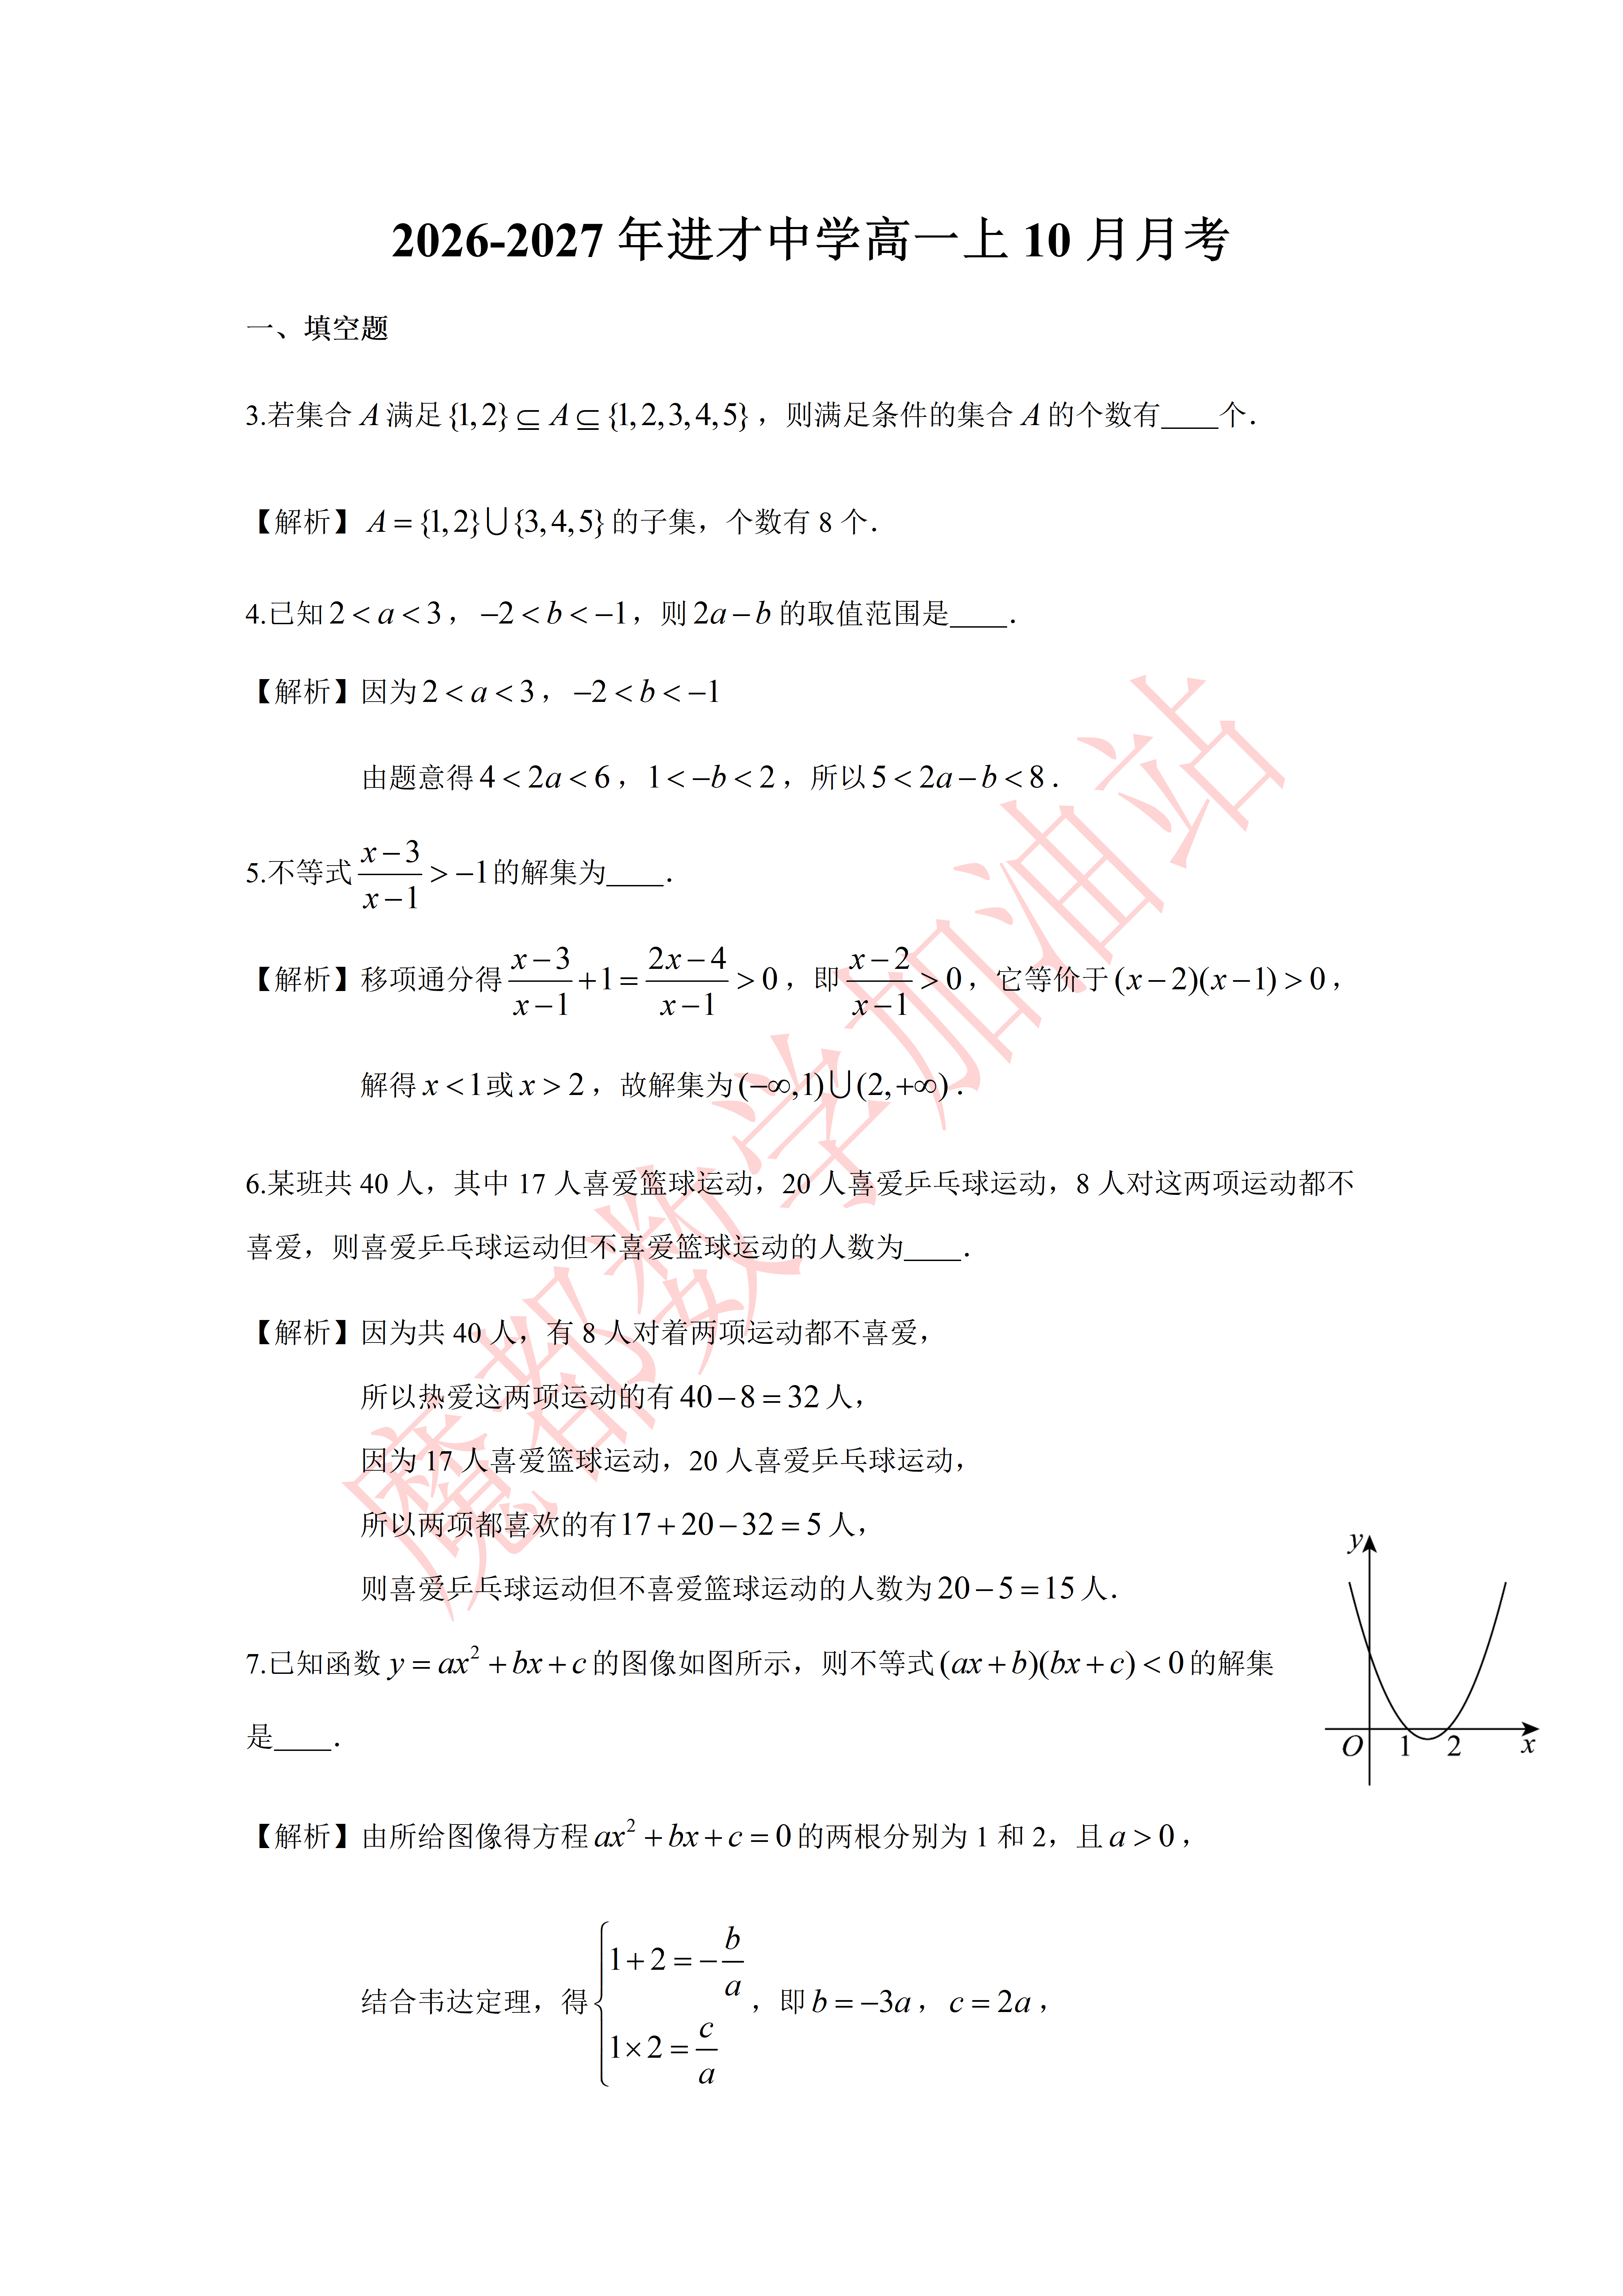
\includegraphics[width=.22\linewidth,trim=3879bp 1490bp 238bp 4492bp,clip]{../原图/高一60_进才中学_10月月考/01.png}
\end{center}

\ifanswer
\solbegin
\step{由所给图像得方程 $ax^2+bx+c=0$ 的两根分别为 1 和 2，且 $a>0$，}
\step{结合韦达定理，得 $\begin{cases}1+2=-\dfrac ba\\ 1\times2=\dfrac ca\end{cases}$，即 $b=-3a$，$c=2a$，}
\step{所以不等式 $(ax+b)(bx+c)<0$ 即 $(ax-3a)(-3ax+2a)<0$，}
\step{化简得 $(x-3)(3x-2)>0$，解得 $x<\dfrac23$ 或 $x>3$，}
\step{所以不等式 $(ax+b)(bx+c)<0$ 的解集是 $(-\infty,\dfrac23)\cup(3,+\infty)$.}
\solend
\fi

\item 已知集合 $A=\{x\mid ax=6\}$，满足 $A\subseteq\Z$，则整数 $a$ 的所有可能取值有\blankline[4.4em]个.

\ifanswer
\solbegin
\step{当 $a=0$ 时，$A=\varnothing$，而 $\varnothing\subseteq\Z$，满足题意，}
\step{当 $a\neq0$ 时，$A=\left\{\dfrac6a\right\}$，要使 $A\subseteq\Z$，则 $\dfrac6a\in\Z$，所以 $a=\pm1,\pm2,\pm3,\pm6$，}
\step{综上，整数 $a$ 的可能取值为 0，$\pm1$，$\pm2$，$\pm3$，$\pm6$，共 9 个.}
\solend
\fi

\item 设关于 $x$ 的方程 $x^2+kx+n=0$ 有两个不同实根 $x_1$、$x_2$，且 $\dfrac1{x_1}+\dfrac1{x_2}=2$，则实数 $n$ 的取值范围是\blankline[4.4em].

\ifanswer
\solbegin
\step{由于方程 $x^2+kx+n=0$ 有两个不同实根 $x_1$、$x_2$，}
\step{因此 $\Delta=k^2-4n>0$，$x_1+x_2=-k$，$x_1x_2=n$，}
\step{由 $\dfrac1{x_1}+\dfrac1{x_2}=\dfrac{x_1+x_2}{x_1x_2}=\dfrac{-k}{n}=2$，得 $k=-2n$，}
\step{因此 $\Delta=k^2-4n=4n^2-4n>0$，解得 $n<0$ 或 $n>1$，}
\step{则实数 $n$ 的取值范围是 $(-\infty,0)\cup(1,+\infty)$.}
\solend
\fi

\item 某船从甲地沿河顺流航行 $75\mathrm{km}$，到达乙码头，停留 $30\mathrm{min}$ 后再逆流航行 $126\mathrm{km}$ 到达丙地，若水流速度为 $4\mathrm{km/h}$，且该船要在 $5\mathrm{h}$ 内完成航行任务，那么船的速度至少达到\blankline[4.4em]$\mathrm{km/h}$.

\ifanswer
\solbegin
\step{设该轮船在静水中的速度是 $x$ 千米/小时，水流速度是 4 千米/小时，}
\step{由题意得 $\dfrac{75}{4+x}+0.5+\dfrac{126}{x-4}\leqslant5$，即 $9x^2-402x-552\geqslant0$，解得 $x\geqslant46$，}
\step{答：该船的速度至少是 46 千米/小时.}
\solend
\fi

\item 设实数 $a,b,c$ 满足 $a^2+b^2\leqslant c<1$，则 $a+\dfrac12b+c$ 的最小值为\blankline[4.4em].

\ifanswer
\solbegin
\step{因为 $c\geqslant a^2+b^2$，}
\step{所以 $a+\dfrac12b+c\geqslant a+\dfrac12b+a^2+b^2=\left(a+\dfrac12\right)^2+\left(b+\dfrac14\right)^2-\dfrac5{16}\geqslant-\dfrac5{16}$，}
\step{当 $a=-\dfrac12,b=-\dfrac14,c=a^2+b^2=\dfrac5{16}$（此时 $c<1$ 成立）时取到等号，}
\step{故最小值为 $-\dfrac5{16}$.}
\solend
\fi

\item 已知集合 $A=\{x\in\N^*\mid1\leqslant x\leqslant2026\}$. 设集合 $B=\{b_1,b_2,b_3,\cdots,b_n\}$ 满足 $B\subseteq A$，且对任意的 $b_i$、$b_j$、$b_k\in B(i$、$j$、$k\in\{1,2,3,\cdots,n\})$，存在 $m\in\N^*$，使得 $b_i+b_j+b_k=39m$，则 $n$ 的最大值为\blankline[4.4em].

\ifanswer
\solbegin
\step{因为 $39=1\times39=3\times13$，所以 $n$ 的最大值大于 3，}
\step{若对任意的 $b_i$、$b_j$、$b_k\in B$，存在 $m\in\N^*$，使得 $b_i+b_j+b_k=39m$，}
\step{则集合 $B$ 的元素除以 39 的余数均为 0 或均为 13 或均为 26，}
\step{即 $B=\{39,78,\cdots,39n\}$ 或 $B=\{13,52,\cdots,39n-26\}$}
\step{或 $B=\{26,65,\cdots,39n-13\}$，}
\step{若 $B=\{39,78,\cdots,39n\}$，则 $39n\leqslant2026$，}
\step{解得 $n\leqslant\dfrac{2026}{39}\in(51,52)$，此时 $n$ 的最大值为 51；}
\step{若 $B=\{13,52,\cdots,39n-26\}$，则 $39n-26\leqslant2026$，}
\step{解得 $n\leqslant\dfrac{684}{13}\in(52,53)$，此时 $n$ 的最大值为 52；}
\step{若 $B=\{26,65,\cdots,39n-13\}$，则 $39n-13\leqslant2026$，}
\step{解得 $n\leqslant\dfrac{2039}{39}\in(52,53)$，此时 $n$ 的最大值为 52；}
\step{综上，$n$ 的最大值为 52.}
\solend
\fi

\end{enumerate}

\bigsec{二、选择题}

\begin{enumerate}
\setcounter{enumi}{12}

% 第 13 题原卷无【答案】/【解析】段，答案“B”直接印在题干括号内，
% 按 高一53 第 13 题的成例括号留空、答案另提为 \ans{}（见文件头）
\item 已知 $a$、$b\in\R$，则“$|a|>|b|$”是“$a>|b|$”的\mbox{（\quad）}

\keepwithprev
A. 充分不必要条件\qquad B. 必要不充分条件

C. 充要条件\qquad D. 既不充分也不必要条件

\ifanswer
\ans{$B$}
\fi

\item 如果关于 $x$ 的一元二次方程 $x^2+2mx+(m+2)=0$ 有一正根一负根，那么 $m$ 的取值范围为\mbox{（\quad）}

\keepwithprev
A. $(-2,-1)$\qquad B. $(-1,2)$

C. $(-\infty,-1)\cup(2,+\infty)$\qquad D. $(-\infty,-2)$

\ifanswer
\solbegin
\step{设两根为 $x_1,x_2$，方程有一正根一负根，则 $\begin{cases}x_1x_2=m+2<0\\ \Delta=4m^2-4(m+2)>0\end{cases}$，}
\step{解得 $m<-2$，故选 $D$.}
\solend
\fi

\item 若不等式 $|3x-a|\leqslant x+2$ 的解集包含集合 $[0,1]$，则实数 $a$ 的取值范围为\mbox{（\quad）}

\keepwithprev
A. $[0,2]$\qquad B. $[0,1]$

C. $[1,2]$\qquad D. $(1,2)$

\ifanswer
\solbegin
% 原卷“法一：”“法二：”排红色加粗（全卷唯一红字），本稿按全稿子题标号样式排 \stepm
% （详见文件头“与原卷的排版差异”⑦）
\stepm{法一：}{不等式 $|3x-a|\leqslant x+2$ 化为 $2x-2\leqslant a\leqslant4x+2$，}
% 原卷此句缺动词（疑漏“对”字），照录未改（见文件头“原卷存疑”④）
\step{$[0,1]$ 使 $2x-2\leqslant a\leqslant4x+2$ 成立，则 $0\leqslant a\leqslant2$，故选 $A$.}
\stepm{法二：}{将两边平方整理得 $8x^2-(6a+4)x+a^2-4\leqslant0$ 对 $[0,1]$ 恒成立，}
\step{则有 $\begin{cases}a^2-4\leqslant0\\ a^2-6a\leqslant0\end{cases}$，解得 $0\leqslant a\leqslant2$，故选 $A$.}
\solend
\fi

\item 数学组 Y 老师在白纸上写下以下四个命题：

①这四个命题中至少有一个是真的；②这四个命题中至少有两个是真的；

③这四个命题中至少有两个是假的；④这四个命题中至少有一个是假的；

每个命题非真即假. 问 Y 老师在纸上写的假命题有几个？\mbox{（\quad）}

\keepwithprev
A. 0\qquad B. 1

C. 2\qquad D. 3

\ifanswer
\solbegin
\step{设四个命题中真命题的个数为 $t$，则①真 $\iff t\geqslant1$，②真 $\iff t\geqslant2$，}
\step{③真 $\iff t\leqslant2$，④真 $\iff t\leqslant3$.}
\step{逐一检验：$t=0$ 时③④为真，应为 $t=2$，矛盾；}
\step{$t=1$ 时①③④为真，应为 $t=3$，矛盾；}
\step{$t=2$ 时四个命题全为真，应为 $t=4$，矛盾；}
\step{$t=3$ 时①②④为真、③为假，恰有 3 个真命题，符合；}
\step{$t=4$ 时①②为真，应为 $t=2$，矛盾.}
\step{所以恰有 1 个假命题，故选 $B$.}
\solend
\fi

\end{enumerate}

\bigsec{三、解答题}

\begin{enumerate}
\setcounter{enumi}{16}

\item 已知：$x\in\R$，$a=x^2-1$，$b=4x+5$. 求证：$a$、$b$ 中至少有一个大于等于 0.

\ifanswer
\solbegin
\step{假设 $a$、$b$ 都小于 0，即 $a<0$，$b<0$，则 $a+b<0$.}
\step{又 $a+b=x^2-1+4x+5=x^2+4x+4=(x+2)^2\geqslant0$，}
\step{这与假设所得 $a+b<0$ 矛盾，故假设不成立，}
\step{所以 $a$、$b$ 中至少有一个大于等于 0.}
\solend
\fi

\ansspace[6]

% 原卷 A、B 两个集合定义之间排半角逗号“,”（5 倍放大核，右侧字距 19px，与全卷全角“，”的 65—79px 字距判然有别）；
% 本稿原误抄为全角“，”——已照录原卷半角（见文件头“与原卷的排版差异”⑤）
\item 已知集合 $A=\{x\mid4\leqslant x\leqslant12\}$,$B=\{x\mid a\leqslant x\leqslant2a+1\}$.

（1）若 $a=2$，求 $\overline A\cap B$；

（2）已知 $A\cup B=A$，求实数 $a$ 的取值范围.

\ifanswer
\solbegin
\stepm{(1)}{当 $a=2$ 时，$B=\{x\mid2\leqslant x\leqslant5\}$，}
\step{而 $A=\{x\mid4\leqslant x\leqslant12\}$，则 $\overline A=(-\infty,4)\cup(12,+\infty)$，所以 $\overline A\cap B=[2,4)$.}
\stepm{(2)}{$A\cup B=A$ 即 $B\subseteq A$.}
\stepm{①}{当 $B=\varnothing$ 时，$a>2a+1$，即 $a<-1$，符合；}
\stepm{②}{当 $B\neq\varnothing$ 时，需 $a\leqslant2a+1$ 且 $a\geqslant4$ 且 $2a+1\leqslant12$，即 $4\leqslant a\leqslant\dfrac{11}2$.}
\step{综上，$a$ 的取值范围是 $(-\infty,-1)\cup\left[4,\dfrac{11}2\right]$.}
\solend
\fi

\ansspace[8]

\item （1）若关于 $x$ 的不等式 $ax^2-3x+2<0$ 的解集不是空集，求实数 $a$ 的取值范围；

（2）求关于 $x$ 的不等式 $ax^2-3x+2>ax-1$ 的解集.

\ifanswer
\solbegin
\stepm{(1)}{若 $a>0$，关于 $x$ 的不等式 $ax^2-3x+2<0$ 的解集不空，}
\step{所以一元二次方程 $ax^2-3x+2=0$ 的判别式大于零，}
\step{即 $(-3)^2-8a>0\Rightarrow a<\dfrac98$，结合 $a>0$ 得 $0<a<\dfrac98$；}
\step{若 $a\leqslant0$，则关于 $x$ 的不等式 $ax^2-3x+2<0$ 的解集不是空集；}
\step{综上，实数 $a$ 的取值范围是 $\left(-\infty,\dfrac98\right)$.}
\stepm{(2)}{$ax^2-3x+2>ax-1\Rightarrow ax^2-(a+3)x+3>0\Rightarrow(ax-3)(x-1)>0$，}
\step{当 $a=0$ 时，不等式为 $x-1<0$，不等式的解集为 $\{x\mid x<1\}$；}
\step{当 $a<0$ 时，不等式化为 $\left(x-\dfrac3a\right)(x-1)<0$，}
\step{不等式的解集为 $\left\{x\mid\dfrac3a<x<1\right\}$，}
\step{当 $a>0$ 时，方程 $ax^2-3x+2=ax-1$ 的两个根分别为：$\dfrac3a,1$.}
\step{当 $a=3$ 时，两根相等，故不等式的解集为 $\{x\mid x\neq1\}$；}
\step{当 $a>3$ 时，$\dfrac3a<1$，不等式的解集为 $\left\{x\mid x<\dfrac3a\right.$ 或 $\left.x>1\right\}$；}
\step{当 $0<a<3$ 时，$\dfrac3a>1$，不等式的解集为 $\left\{x\mid x<1\right.$ 或 $\left.x>\dfrac3a\right\}$；}
\step{综上所述，当 $a<0$ 时，不等式的解集为 $\left\{x\mid\dfrac3a<x<1\right\}$，}
\step{当 $a=0$ 时，不等式的解集为 $\{x\mid x<1\}$，}
\step{当 $0<a<3$ 时，不等式的解集为 $\left\{x\mid x<1\right.$ 或 $\left.x>\dfrac3a\right\}$，}
\step{当 $a=3$ 时，不等式的解集为 $\{x\mid x\neq1\}$，}
\step{当 $a>3$ 时，不等式的解集为 $\left\{x\mid x<\dfrac3a\right.$ 或 $\left.x>1\right\}$.}
\solend
\fi

\ansspace[8]

\item 设命题 $p$：对任意 $x\in\R$，使得不等式 $mx^2-mx+2>0$ 恒成立；命题 $q$：存在 $0\leqslant x\leqslant3$，不等式 $2x-2\geqslant|m|$ 成立.

（1）若 $p$ 为真命题，求实数 $m$ 的取值范围；

（2）若 $p$、$q$ 有且只有一个是真命题，求实数 $m$ 的取值范围.

\ifanswer
\solbegin
\stepm{(1)}{因为 $p:\forall x\in\R$，$mx^2-mx+2>0$ 为真命题，}
\step{所以当 $m=0$ 时，不等式为 $2>0$，在 $\R$ 上恒成立，符合题意；}
\step{当 $m\neq0$ 时，$\begin{cases}m>0\\ \Delta=m^2-8m<0\end{cases}$，解得 $0<m<8$.}
\step{综上，实数 $m$ 的取值范围为 $[0,8)$.}
\stepm{(2)}{若 $q$ 为真命题，即 $q:\exists0\leqslant x\leqslant3$，$2x-2\geqslant|m|$，}
\step{则对于 $0\leqslant x\leqslant3$，$(2x-2)_{max}\geqslant|m|$.}
\step{由于 $0\leqslant x\leqslant3$，$2x-2\in[-2,4]$，所以 $|m|\leqslant4$，解得 $-4\leqslant m\leqslant4$，}
\step{又因为 $p$、$q$ 有且只有一个是真命题，}
\step{所以当 $p$ 真 $q$ 假时，$\begin{cases}0\leqslant m<8\\ m<-4\text{或}m>4\end{cases}$，解得 $4<m<8$；}
\step{当 $p$ 假 $q$ 真时，$\begin{cases}m<0\text{或}m\geqslant8\\ -4\leqslant m\leqslant4\end{cases}$，解得 $-4\leqslant m<0$；}
\step{综上，实数 $m$ 的取值范围为 $[-4,0)\cup(4,8)$.}
\solend
\fi

\ansspace[10]

\item 已知集合 $A=\{a_1,a_2,\cdots,a_k\}(k\geqslant2)$. 其中 $a_i\in\N^*(i=1,2,\cdots,k)$. 若对于任意的 $a\in A$，总有 $\dfrac1a\notin A$，则称集合 $A$ 具有性质 $P$. 由 $A$ 中的元素构成两个相应的集合：$S=\{(a,b)\mid a\in A,b\in A,ab\in A\}$，$T=\left\{(a,b)\mid a\in A,b\in A,\dfrac ab\in A\right\}$，其中 $(a,b)$ 是有序数对，集合 $S$ 和 $T$ 中的元素个数分别为 $m$ 和 $n$.

（1）检验集合 $\{2,3,6\}$ 与 $\{1,2,4\}$ 是否具有性质 $P$，并对其中具有性质 $P$ 的集合，写出相应的集合 $S$ 和 $T$；

（2）对任何具有性质 $P$ 的集合 $A$，$n$ 的最大值为多少？（直接写出答案，无需说明理由）；

% 原卷题干的小问编号跳号：印作 (1)(2)(4)，本稿照录 (4)、未改成 (3)（见文件头“原卷存疑”①）
（4）判断 $m$ 和 $n$ 的大小关系，并证明你的结论.

\ifanswer
\solbegin
\stepm{(1)}{因为 $\dfrac12\in\{1,2,4\}$，所以 $\{1,2,4\}$ 不具有性质 $P$；}
\step{因为 $\dfrac12\notin\{2,3,6\}$，$\dfrac13\notin\{2,3,6\}$，$\dfrac16\notin\{2,3,6\}$，所以 $\{2,3,6\}$ 具有性质 $P$.}
\step{$S=\{(2,3),(3,2)\}$，$T=\{(6,2),(6,3)\}$；}
\stepm{(2)}{因为对于任意的 $a\in A$，总有 $\dfrac1a\notin A$，所以 $1\notin A$，}
% 原卷此处印作“$\{(a_i,a_i)\}\in T$”，与上一句“$1\notin A$”及下文“最多为 $C_k^2$”的推理
% 均不自洽（应为“$\notin$”），已 8 倍放大确认无斜线；照录未改（见文件头“原卷存疑”③）
\step{从而 $\{(a_i,a_i)\}\in T(i=1,2,\cdots,k)$.}
\step{因为 $a\in A,b\in A,\dfrac ab\in A$，所以当 $i\neq j$ 时，}
\step{$(a_i,a_j)\in T$ 和 $(a_j,a_i)\in T(i,j=1,2,\cdots,k)$ 至多有一个成立，}
\step{所以集合 $T$ 中的元素个数最多为 $C_k^2=\dfrac{k(k-1)}2$，即 $n\leqslant\dfrac{k(k-1)}2$.}
% 原卷【解析】把第 (4) 问标作“(3)”（与题干跳号相应），本稿照录未改（见文件头“原卷存疑”①）
\stepm{(3)}{$m=n$，证明如下：}
\step{①设 $(a,b)\in T$，则 $a\in A,b\in A,\dfrac ab\in A$. 设 $c=\dfrac ab$，则 $a=bc$，}
\step{故 $b\in A$，$c\in A$，$bc\in A$，从而 $(b,c)\in S$，}
\step{即对 $\forall(a,b)\in T$，总 $\exists c$ 使 $(b,c)\in S$，从而 $n\leqslant m$.}
\step{②设 $(p,q)\in S$，则 $p\in A$，$q\in A$，$pq\in A$.}
\step{设 $r=pq$，则 $q=\dfrac rp$，故 $r\in A,p\in A,\dfrac rp\in A$，从而 $(r,p)\in T$，}
\step{即对 $\forall(p,q)\in S$，总 $\exists r$ 使 $(r,p)\in T$，从而 $m\leqslant n$.}
\step{由①②得 $m=n$.}
\solend
\fi

\ansspace*[10]

\end{enumerate}

\end{document}
"
%
% 原文链接：https://mp.weixin.qq.com/s/2ZLKB3IONEDhcUAfAAYE2A。
% 公众号“魔都数学加油站”作者破晓于 2026-10-14 22:15 发布。
% 原图 9 张（`原图/高一60_进才中学_10月月考/01..09.png`）：第 1—8 页 4762×6735，
% 第 9 页 2560×3620（同一篇内两档分辨率）。
%
% 卷首标题：照卷面印作“2026--2027 年进才中学高一上 10 月月考”（公众号标题中的“上海市”
% 卷面标题行没有，本稿照卷面），年份区间按全稿惯例排 en dash。原卷只有一行标题、无副标题。
%
% 篇幅与题号：原卷自第 3 题起编号（第 1、2 题不在本卷内）。填空题 3—12（10 题）、
% 选择题 13—16（4 题）、解答题 17—21（5 题），共 19 题。本稿沿用原节与原题号，
% 只改排为全稿统一的大节样式（原卷小节标题为“一、填空题”“二、选择题”“三、解答题”）。
%
% 讲评版：原卷每题下直接印【答案】或【解析】。**只印【解析】的 18 题**，本稿按全稿口径
% 收进答案版、不另提 \ans{}——第 14、15、16 题的结论写在解析末句（“故选 D／A／B”），
% 亦照录在解析内。**第 13 题原卷没有任何【答案】/【解析】段**，答案“B”直接印在题干括号内
% （“（ B ）”），本稿按 高一53 第 13 题的成例把括号留空、答案另提为 \ans{$B$}（见下）。
%
% 副标题：原卷未印副标题。本稿按“知识模块”口径标作“集合与常用逻辑用语、不等式”：
% 19 题中集合与常用逻辑用语 10 题（第 3、6、8、12、13、16、17、18、20、21 题，
% 含子集计数、韦恩图容斥、集合运算、命题与充要条件、反证法、新定义），
% 不等式 9 题（含不等式性质、分式不等式、二次函数与解集、韦达定理与判别式、
% 不等式应用、最值、根的分布、绝对值不等式恒成立、含参二次不等式：第 4、5、7、9、10、
% 11、14、15、19 题），两类均远超三分之一，故并标。口径同 高一46、高一47、高一48、
% 高一51—高一59。
%
% 与原卷的排版差异：
%   ① 原卷每题下直接印【答案】/【解析】，本稿按全稿惯例将答案与解析置于答案版，试卷版保持干净；
%   ② 原卷未印副标题，本稿按“知识模块”口径补出；
%   ③ 原卷填空横线约两个字宽，本稿按全稿惯例统一排 \blankline[4.4em]；
%   ④ 原卷实数集排斜体 $R$（第 13、17、20 题）、正整数集排 $N^*$（第 12、21 题）、
%      整数集排粗体 $\mathbf{Z}$（第 8 题），本稿按全稿惯例改用 $\R$、$\N^*$、$\Z$；
%      空集记号统一为 \varnothing；
%   ⑤ 原卷在数学式内多处用半角逗号（如 $x_1,x_2$、$a,b\in R$，以及第 18 题题干
%      $A=\{x\mid4\leqslant x\leqslant12\}$,$B=\{x\mid a\leqslant x\leqslant2a+1\}$ 之间的逗号），
%      均照录未强改（第 18 题题干那一处本稿首轮曾误作全角“，”，第二轮已订正）；
%      句末句点按全稿惯例排西文句点；
%   ⑥ 第 13 题印在题干括号内的答案“B”移入 \ans{}，见上；
%   ⑦ 第 15 题【解析】的“法一：”“法二：”标号原卷排**红色加粗**（全卷唯一的红字，2 处），
%      本稿按全稿子题标号样式排 \stepm{法一：}{…}、\stepm{法二：}{…}（加粗着色、不改黑色
%      基调），冒号照原卷排全角；
%   ⑧ 第 7 题的图像原卷排在题干右侧（与题干第 1 行同高），本稿居中排在题干之后；
%      图自原图第 01 页裁切（trim），不另存图片文件；
%   ⑨ 原卷第 10 题的长度与速度单位原卷排斜体（$75km$、$4km/h$ 等），本稿按全稿惯例
%      改排正体 $\mathrm{km}$、$\mathrm{km/h}$（同 高一56 第 13 题）；每道解答题原卷未留
%      作答空白，本稿按全稿惯例加 \ansspace。
%
% 原卷存疑（照录未改，见源码中该处上方注释）：
%   ① 第 21 题题干的小问编号**跳号**：印作 (1)(2)(4)，而紧随其后的【解析】按 (1)(2)(3) 写
%      —— 题干第 (4) 问实为第 (3) 问。本稿题干照录 (1)(2)(4)、解析照录 (3)，未改
%      （与 高一22 第 16 题“解析误标 (2)”同一处理）。
%   ② 第 6 题【解析】“有 8 人**对着**两项运动都不喜爱”，“对着”疑为“对这”之误，照录未改。
%   ③ 第 21(2) 题【解析】首行“所以 $1\notin A$，从而 $\{(a_i,a_i)\}\in T(i=1,2,\cdots,k)$”
%      —— 由 $1\notin A$ 应得 $(a_i,a_i)\notin T$（因 $a_i/a_i=1$），与紧随的“$T$ 中元素
%      个数最多为 $C_k^2$”这一推理亦只有“$\notin$”才自洽；原卷此处印作“$\in$”，
%      已 8 倍放大确认无斜线。**照录原卷的 $\in$、未改**。
%   ④ 第 15 题【解析】法一“$[0,1]$ 使 $2x-2\leqslant a\leqslant4x+2$ 成立”一句缺动词
%      （疑漏“对”字），照录未改。
%
\documentclass[a4paper,11pt]{article}
\usepackage{common}

\begin{document}

\examtitlest[3]{2026--2027 年进才中学高一上 10 月月考}{集合与常用逻辑用语、不等式}

\bigsec{一、填空题}

\begin{enumerate}
\setcounter{enumi}{2}

\item 若集合 $A$ 满足 $\{1,2\}\subseteq A\subseteq\{1,2,3,4,5\}$，则满足条件的集合 $A$ 的个数有\blankline[4.4em]个.

\ifanswer
\solbegin
\step{$A=\{1,2\}\cup\{3,4,5\}$ 的子集，个数有 8 个.}
\solend
\fi

\item 已知 $2<a<3$，$-2<b<-1$，则 $2a-b$ 的取值范围是\blankline[4.4em].

\ifanswer
\solbegin
\step{因为 $2<a<3$，$-2<b<-1$，}
\step{由题意得 $4<2a<6$，$1<-b<2$，所以 $5<2a-b<8$.}
\solend
\fi

\item 不等式 $\dfrac{x-3}{x-1}>-1$ 的解集为\blankline[4.4em].

\ifanswer
\solbegin
\step{移项通分得 $\dfrac{x-3}{x-1}+1=\dfrac{2x-4}{x-1}>0$，即 $\dfrac{x-2}{x-1}>0$，它等价于 $(x-2)(x-1)>0$，}
\step{解得 $x<1$ 或 $x>2$，故解集为 $(-\infty,1)\cup(2,+\infty)$.}
\solend
\fi

\item 某班共 40 人，其中 17 人喜爱篮球运动，20 人喜爱乒乓球运动，8 人对这两项运动都不喜爱，则喜爱乒乓球运动但不喜爱篮球运动的人数为\blankline[4.4em].

\ifanswer
\solbegin
% 原卷作“对着两项运动都不喜爱”（疑为“对这”之误），照录未改（见文件头“原卷存疑”②）
\step{因为共 40 人，有 8 人对着两项运动都不喜爱，}
\step{所以热爱这两项运动的有 $40-8=32$ 人，}
\step{因为 17 人喜爱篮球运动，20 人喜爱乒乓球运动，}
\step{所以两项都喜欢的有 $17+20-32=5$ 人，}
\step{则喜爱乒乓球运动但不喜爱篮球运动的人数为 $20-5=15$ 人.}
\solend
\fi

\item 已知函数 $y=ax^2+bx+c$ 的图像如图所示，则不等式 $(ax+b)(bx+c)<0$ 的解集是\blankline[4.4em].

% 原图第 01 页题干右侧的图像直接裁取。裁框取图外框 x 3887–4516、y 4500–5237
% （四周各留约 8px），trim=左 3879bp／下 1490bp／右 238bp／上 4492bp
% （页宽 4762、页高 6735）。
\begin{center}
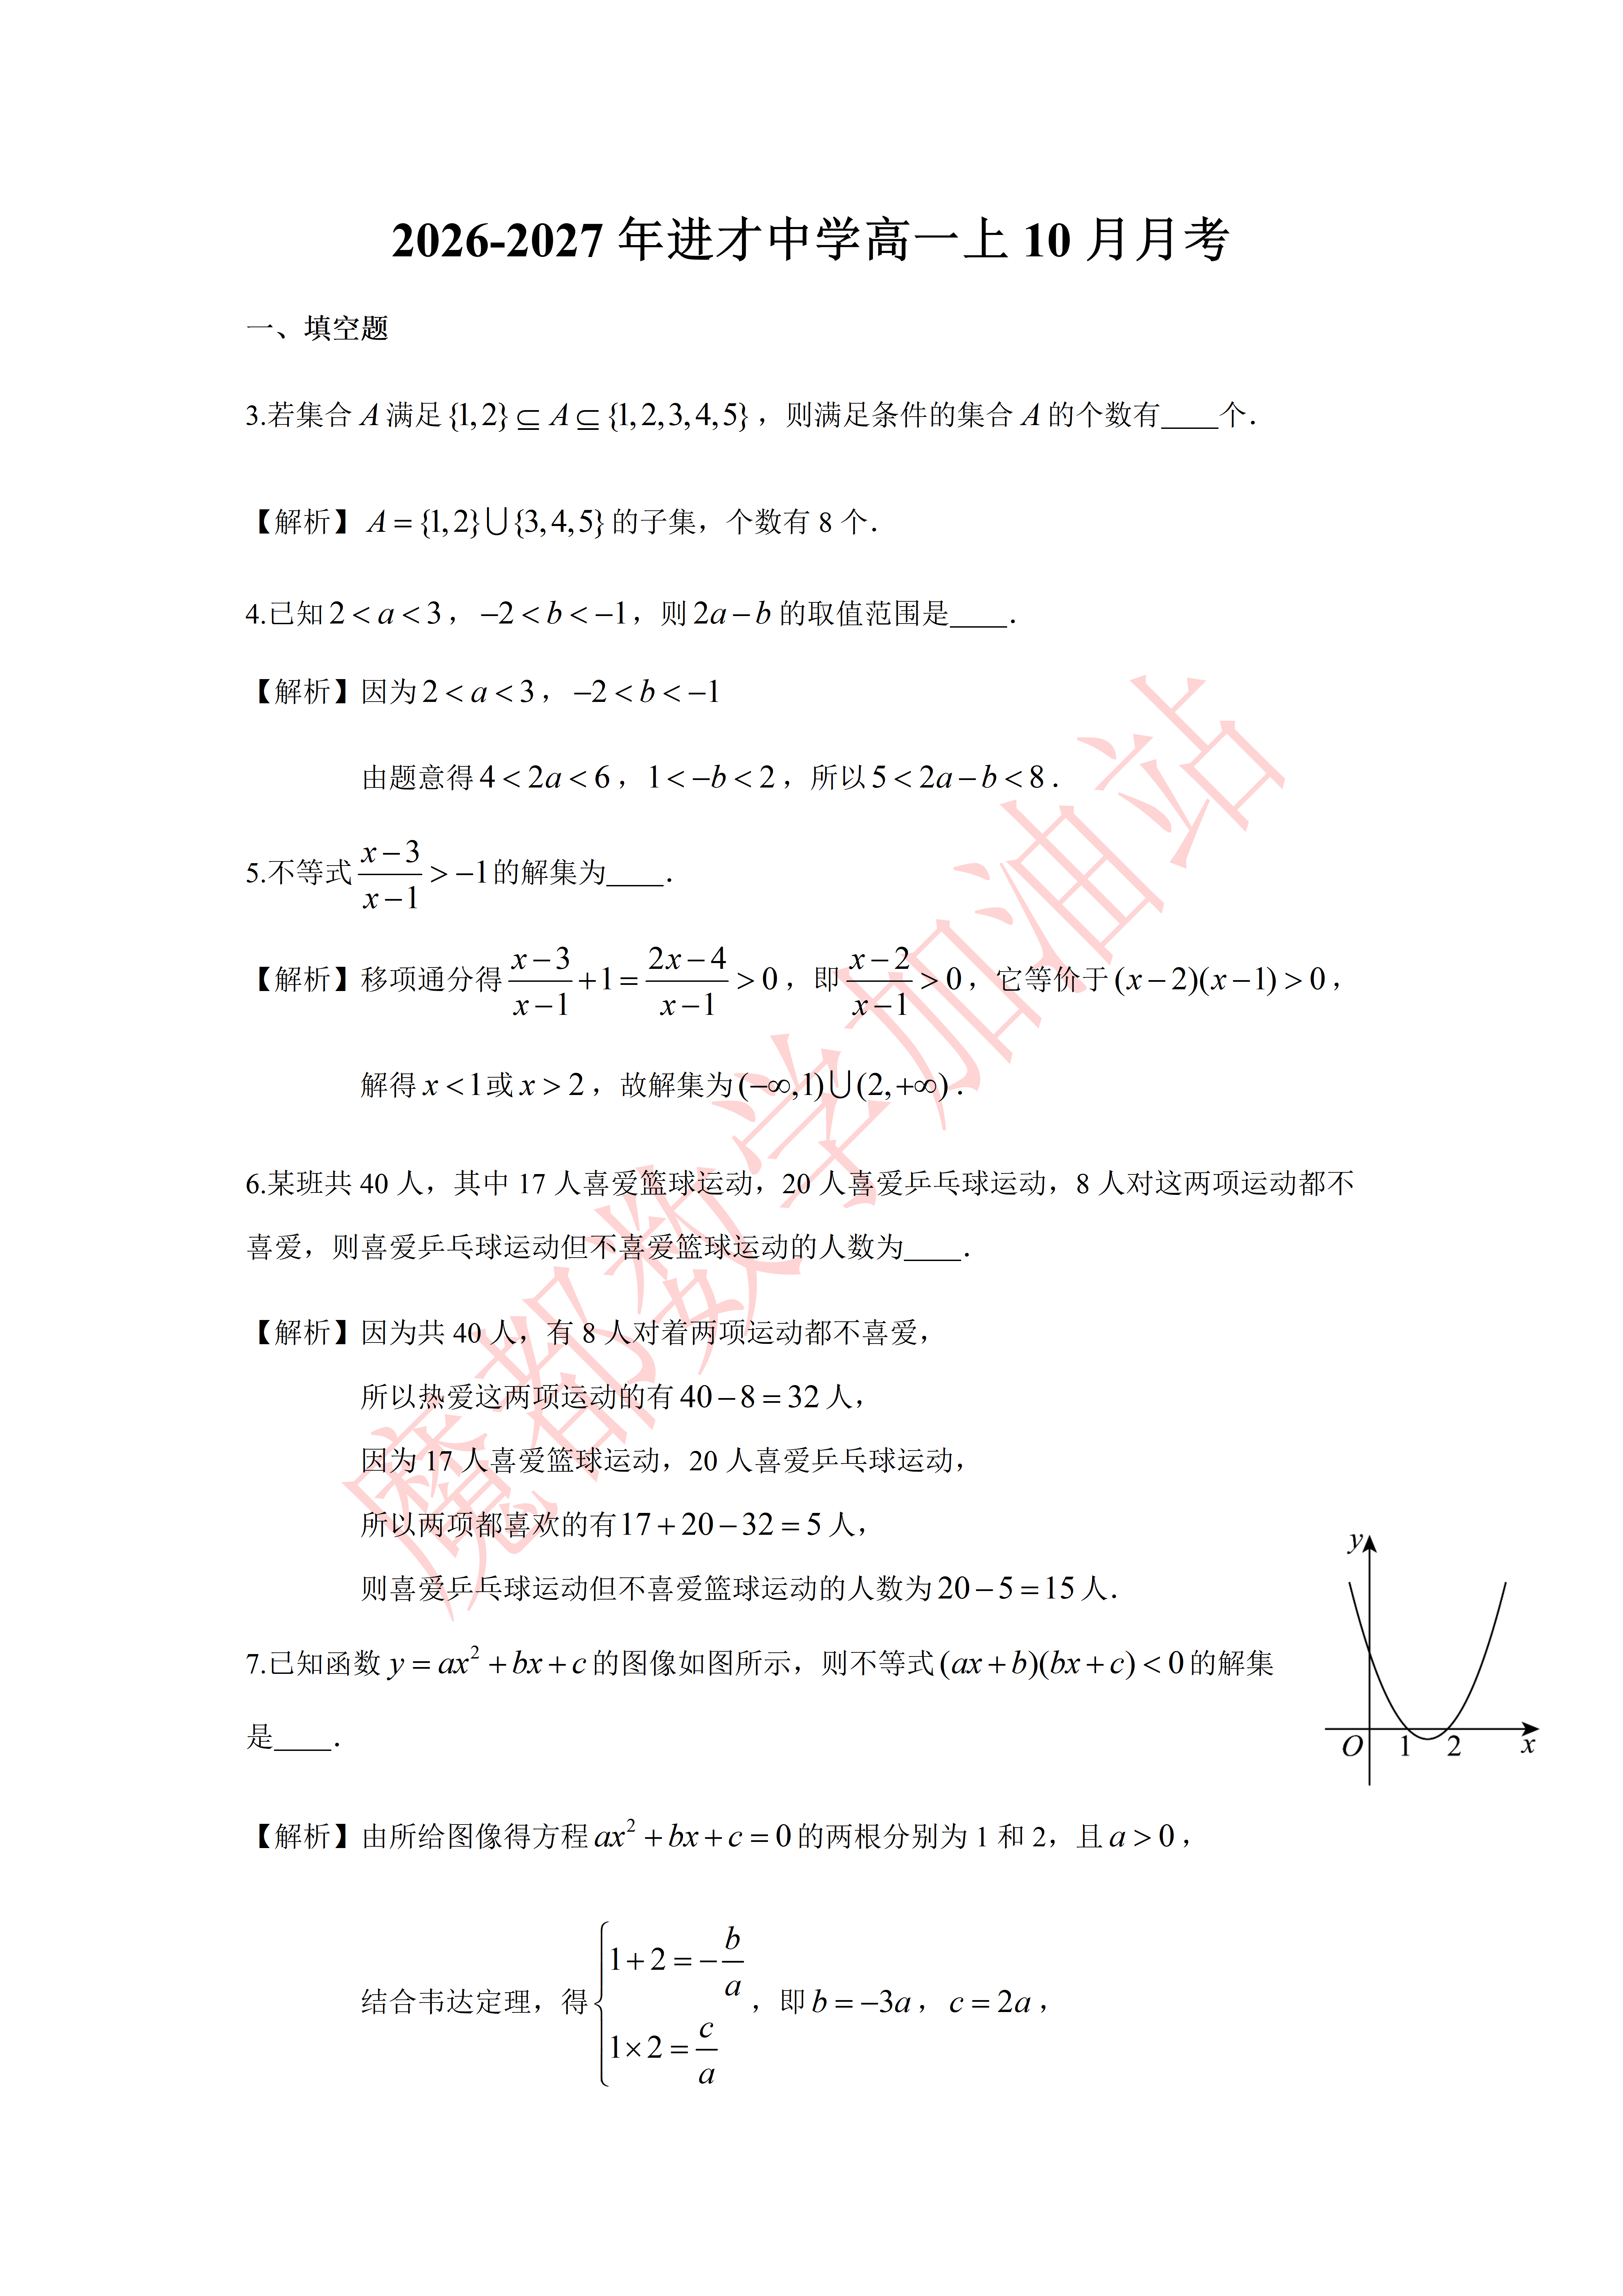
\includegraphics[width=.22\linewidth,trim=3879bp 1490bp 238bp 4492bp,clip]{../原图/高一60_进才中学_10月月考/01.png}
\end{center}

\ifanswer
\solbegin
\step{由所给图像得方程 $ax^2+bx+c=0$ 的两根分别为 1 和 2，且 $a>0$，}
\step{结合韦达定理，得 $\begin{cases}1+2=-\dfrac ba\\ 1\times2=\dfrac ca\end{cases}$，即 $b=-3a$，$c=2a$，}
\step{所以不等式 $(ax+b)(bx+c)<0$ 即 $(ax-3a)(-3ax+2a)<0$，}
\step{化简得 $(x-3)(3x-2)>0$，解得 $x<\dfrac23$ 或 $x>3$，}
\step{所以不等式 $(ax+b)(bx+c)<0$ 的解集是 $(-\infty,\dfrac23)\cup(3,+\infty)$.}
\solend
\fi

\item 已知集合 $A=\{x\mid ax=6\}$，满足 $A\subseteq\Z$，则整数 $a$ 的所有可能取值有\blankline[4.4em]个.

\ifanswer
\solbegin
\step{当 $a=0$ 时，$A=\varnothing$，而 $\varnothing\subseteq\Z$，满足题意，}
\step{当 $a\neq0$ 时，$A=\left\{\dfrac6a\right\}$，要使 $A\subseteq\Z$，则 $\dfrac6a\in\Z$，所以 $a=\pm1,\pm2,\pm3,\pm6$，}
\step{综上，整数 $a$ 的可能取值为 0，$\pm1$，$\pm2$，$\pm3$，$\pm6$，共 9 个.}
\solend
\fi

\item 设关于 $x$ 的方程 $x^2+kx+n=0$ 有两个不同实根 $x_1$、$x_2$，且 $\dfrac1{x_1}+\dfrac1{x_2}=2$，则实数 $n$ 的取值范围是\blankline[4.4em].

\ifanswer
\solbegin
\step{由于方程 $x^2+kx+n=0$ 有两个不同实根 $x_1$、$x_2$，}
\step{因此 $\Delta=k^2-4n>0$，$x_1+x_2=-k$，$x_1x_2=n$，}
\step{由 $\dfrac1{x_1}+\dfrac1{x_2}=\dfrac{x_1+x_2}{x_1x_2}=\dfrac{-k}{n}=2$，得 $k=-2n$，}
\step{因此 $\Delta=k^2-4n=4n^2-4n>0$，解得 $n<0$ 或 $n>1$，}
\step{则实数 $n$ 的取值范围是 $(-\infty,0)\cup(1,+\infty)$.}
\solend
\fi

\item 某船从甲地沿河顺流航行 $75\mathrm{km}$，到达乙码头，停留 $30\mathrm{min}$ 后再逆流航行 $126\mathrm{km}$ 到达丙地，若水流速度为 $4\mathrm{km/h}$，且该船要在 $5\mathrm{h}$ 内完成航行任务，那么船的速度至少达到\blankline[4.4em]$\mathrm{km/h}$.

\ifanswer
\solbegin
\step{设该轮船在静水中的速度是 $x$ 千米/小时，水流速度是 4 千米/小时，}
\step{由题意得 $\dfrac{75}{4+x}+0.5+\dfrac{126}{x-4}\leqslant5$，即 $9x^2-402x-552\geqslant0$，解得 $x\geqslant46$，}
\step{答：该船的速度至少是 46 千米/小时.}
\solend
\fi

\item 设实数 $a,b,c$ 满足 $a^2+b^2\leqslant c<1$，则 $a+\dfrac12b+c$ 的最小值为\blankline[4.4em].

\ifanswer
\solbegin
\step{因为 $c\geqslant a^2+b^2$，}
\step{所以 $a+\dfrac12b+c\geqslant a+\dfrac12b+a^2+b^2=\left(a+\dfrac12\right)^2+\left(b+\dfrac14\right)^2-\dfrac5{16}\geqslant-\dfrac5{16}$，}
\step{当 $a=-\dfrac12,b=-\dfrac14,c=a^2+b^2=\dfrac5{16}$（此时 $c<1$ 成立）时取到等号，}
\step{故最小值为 $-\dfrac5{16}$.}
\solend
\fi

\item 已知集合 $A=\{x\in\N^*\mid1\leqslant x\leqslant2026\}$. 设集合 $B=\{b_1,b_2,b_3,\cdots,b_n\}$ 满足 $B\subseteq A$，且对任意的 $b_i$、$b_j$、$b_k\in B(i$、$j$、$k\in\{1,2,3,\cdots,n\})$，存在 $m\in\N^*$，使得 $b_i+b_j+b_k=39m$，则 $n$ 的最大值为\blankline[4.4em].

\ifanswer
\solbegin
\step{因为 $39=1\times39=3\times13$，所以 $n$ 的最大值大于 3，}
\step{若对任意的 $b_i$、$b_j$、$b_k\in B$，存在 $m\in\N^*$，使得 $b_i+b_j+b_k=39m$，}
\step{则集合 $B$ 的元素除以 39 的余数均为 0 或均为 13 或均为 26，}
\step{即 $B=\{39,78,\cdots,39n\}$ 或 $B=\{13,52,\cdots,39n-26\}$}
\step{或 $B=\{26,65,\cdots,39n-13\}$，}
\step{若 $B=\{39,78,\cdots,39n\}$，则 $39n\leqslant2026$，}
\step{解得 $n\leqslant\dfrac{2026}{39}\in(51,52)$，此时 $n$ 的最大值为 51；}
\step{若 $B=\{13,52,\cdots,39n-26\}$，则 $39n-26\leqslant2026$，}
\step{解得 $n\leqslant\dfrac{684}{13}\in(52,53)$，此时 $n$ 的最大值为 52；}
\step{若 $B=\{26,65,\cdots,39n-13\}$，则 $39n-13\leqslant2026$，}
\step{解得 $n\leqslant\dfrac{2039}{39}\in(52,53)$，此时 $n$ 的最大值为 52；}
\step{综上，$n$ 的最大值为 52.}
\solend
\fi

\end{enumerate}

\bigsec{二、选择题}

\begin{enumerate}
\setcounter{enumi}{12}

% 第 13 题原卷无【答案】/【解析】段，答案“B”直接印在题干括号内，
% 按 高一53 第 13 题的成例括号留空、答案另提为 \ans{}（见文件头）
\item 已知 $a$、$b\in\R$，则“$|a|>|b|$”是“$a>|b|$”的\mbox{（\quad）}

\keepwithprev
A. 充分不必要条件\qquad B. 必要不充分条件

C. 充要条件\qquad D. 既不充分也不必要条件

\ifanswer
\ans{$B$}
\fi

\item 如果关于 $x$ 的一元二次方程 $x^2+2mx+(m+2)=0$ 有一正根一负根，那么 $m$ 的取值范围为\mbox{（\quad）}

\keepwithprev
A. $(-2,-1)$\qquad B. $(-1,2)$

C. $(-\infty,-1)\cup(2,+\infty)$\qquad D. $(-\infty,-2)$

\ifanswer
\solbegin
\step{设两根为 $x_1,x_2$，方程有一正根一负根，则 $\begin{cases}x_1x_2=m+2<0\\ \Delta=4m^2-4(m+2)>0\end{cases}$，}
\step{解得 $m<-2$，故选 $D$.}
\solend
\fi

\item 若不等式 $|3x-a|\leqslant x+2$ 的解集包含集合 $[0,1]$，则实数 $a$ 的取值范围为\mbox{（\quad）}

\keepwithprev
A. $[0,2]$\qquad B. $[0,1]$

C. $[1,2]$\qquad D. $(1,2)$

\ifanswer
\solbegin
% 原卷“法一：”“法二：”排红色加粗（全卷唯一红字），本稿按全稿子题标号样式排 \stepm
% （详见文件头“与原卷的排版差异”⑦）
\stepm{法一：}{不等式 $|3x-a|\leqslant x+2$ 化为 $2x-2\leqslant a\leqslant4x+2$，}
% 原卷此句缺动词（疑漏“对”字），照录未改（见文件头“原卷存疑”④）
\step{$[0,1]$ 使 $2x-2\leqslant a\leqslant4x+2$ 成立，则 $0\leqslant a\leqslant2$，故选 $A$.}
\stepm{法二：}{将两边平方整理得 $8x^2-(6a+4)x+a^2-4\leqslant0$ 对 $[0,1]$ 恒成立，}
\step{则有 $\begin{cases}a^2-4\leqslant0\\ a^2-6a\leqslant0\end{cases}$，解得 $0\leqslant a\leqslant2$，故选 $A$.}
\solend
\fi

\item 数学组 Y 老师在白纸上写下以下四个命题：

①这四个命题中至少有一个是真的；②这四个命题中至少有两个是真的；

③这四个命题中至少有两个是假的；④这四个命题中至少有一个是假的；

每个命题非真即假. 问 Y 老师在纸上写的假命题有几个？\mbox{（\quad）}

\keepwithprev
A. 0\qquad B. 1

C. 2\qquad D. 3

\ifanswer
\solbegin
\step{设四个命题中真命题的个数为 $t$，则①真 $\iff t\geqslant1$，②真 $\iff t\geqslant2$，}
\step{③真 $\iff t\leqslant2$，④真 $\iff t\leqslant3$.}
\step{逐一检验：$t=0$ 时③④为真，应为 $t=2$，矛盾；}
\step{$t=1$ 时①③④为真，应为 $t=3$，矛盾；}
\step{$t=2$ 时四个命题全为真，应为 $t=4$，矛盾；}
\step{$t=3$ 时①②④为真、③为假，恰有 3 个真命题，符合；}
\step{$t=4$ 时①②为真，应为 $t=2$，矛盾.}
\step{所以恰有 1 个假命题，故选 $B$.}
\solend
\fi

\end{enumerate}

\bigsec{三、解答题}

\begin{enumerate}
\setcounter{enumi}{16}

\item 已知：$x\in\R$，$a=x^2-1$，$b=4x+5$. 求证：$a$、$b$ 中至少有一个大于等于 0.

\ifanswer
\solbegin
\step{假设 $a$、$b$ 都小于 0，即 $a<0$，$b<0$，则 $a+b<0$.}
\step{又 $a+b=x^2-1+4x+5=x^2+4x+4=(x+2)^2\geqslant0$，}
\step{这与假设所得 $a+b<0$ 矛盾，故假设不成立，}
\step{所以 $a$、$b$ 中至少有一个大于等于 0.}
\solend
\fi

\ansspace[6]

% 原卷 A、B 两个集合定义之间排半角逗号“,”（5 倍放大核，右侧字距 19px，与全卷全角“，”的 65—79px 字距判然有别）；
% 本稿原误抄为全角“，”——已照录原卷半角（见文件头“与原卷的排版差异”⑤）
\item 已知集合 $A=\{x\mid4\leqslant x\leqslant12\}$,$B=\{x\mid a\leqslant x\leqslant2a+1\}$.

（1）若 $a=2$，求 $\overline A\cap B$；

（2）已知 $A\cup B=A$，求实数 $a$ 的取值范围.

\ifanswer
\solbegin
\stepm{(1)}{当 $a=2$ 时，$B=\{x\mid2\leqslant x\leqslant5\}$，}
\step{而 $A=\{x\mid4\leqslant x\leqslant12\}$，则 $\overline A=(-\infty,4)\cup(12,+\infty)$，所以 $\overline A\cap B=[2,4)$.}
\stepm{(2)}{$A\cup B=A$ 即 $B\subseteq A$.}
\stepm{①}{当 $B=\varnothing$ 时，$a>2a+1$，即 $a<-1$，符合；}
\stepm{②}{当 $B\neq\varnothing$ 时，需 $a\leqslant2a+1$ 且 $a\geqslant4$ 且 $2a+1\leqslant12$，即 $4\leqslant a\leqslant\dfrac{11}2$.}
\step{综上，$a$ 的取值范围是 $(-\infty,-1)\cup\left[4,\dfrac{11}2\right]$.}
\solend
\fi

\ansspace[8]

\item （1）若关于 $x$ 的不等式 $ax^2-3x+2<0$ 的解集不是空集，求实数 $a$ 的取值范围；

（2）求关于 $x$ 的不等式 $ax^2-3x+2>ax-1$ 的解集.

\ifanswer
\solbegin
\stepm{(1)}{若 $a>0$，关于 $x$ 的不等式 $ax^2-3x+2<0$ 的解集不空，}
\step{所以一元二次方程 $ax^2-3x+2=0$ 的判别式大于零，}
\step{即 $(-3)^2-8a>0\Rightarrow a<\dfrac98$，结合 $a>0$ 得 $0<a<\dfrac98$；}
\step{若 $a\leqslant0$，则关于 $x$ 的不等式 $ax^2-3x+2<0$ 的解集不是空集；}
\step{综上，实数 $a$ 的取值范围是 $\left(-\infty,\dfrac98\right)$.}
\stepm{(2)}{$ax^2-3x+2>ax-1\Rightarrow ax^2-(a+3)x+3>0\Rightarrow(ax-3)(x-1)>0$，}
\step{当 $a=0$ 时，不等式为 $x-1<0$，不等式的解集为 $\{x\mid x<1\}$；}
\step{当 $a<0$ 时，不等式化为 $\left(x-\dfrac3a\right)(x-1)<0$，}
\step{不等式的解集为 $\left\{x\mid\dfrac3a<x<1\right\}$，}
\step{当 $a>0$ 时，方程 $ax^2-3x+2=ax-1$ 的两个根分别为：$\dfrac3a,1$.}
\step{当 $a=3$ 时，两根相等，故不等式的解集为 $\{x\mid x\neq1\}$；}
\step{当 $a>3$ 时，$\dfrac3a<1$，不等式的解集为 $\left\{x\mid x<\dfrac3a\right.$ 或 $\left.x>1\right\}$；}
\step{当 $0<a<3$ 时，$\dfrac3a>1$，不等式的解集为 $\left\{x\mid x<1\right.$ 或 $\left.x>\dfrac3a\right\}$；}
\step{综上所述，当 $a<0$ 时，不等式的解集为 $\left\{x\mid\dfrac3a<x<1\right\}$，}
\step{当 $a=0$ 时，不等式的解集为 $\{x\mid x<1\}$，}
\step{当 $0<a<3$ 时，不等式的解集为 $\left\{x\mid x<1\right.$ 或 $\left.x>\dfrac3a\right\}$，}
\step{当 $a=3$ 时，不等式的解集为 $\{x\mid x\neq1\}$，}
\step{当 $a>3$ 时，不等式的解集为 $\left\{x\mid x<\dfrac3a\right.$ 或 $\left.x>1\right\}$.}
\solend
\fi

\ansspace[8]

\item 设命题 $p$：对任意 $x\in\R$，使得不等式 $mx^2-mx+2>0$ 恒成立；命题 $q$：存在 $0\leqslant x\leqslant3$，不等式 $2x-2\geqslant|m|$ 成立.

（1）若 $p$ 为真命题，求实数 $m$ 的取值范围；

（2）若 $p$、$q$ 有且只有一个是真命题，求实数 $m$ 的取值范围.

\ifanswer
\solbegin
\stepm{(1)}{因为 $p:\forall x\in\R$，$mx^2-mx+2>0$ 为真命题，}
\step{所以当 $m=0$ 时，不等式为 $2>0$，在 $\R$ 上恒成立，符合题意；}
\step{当 $m\neq0$ 时，$\begin{cases}m>0\\ \Delta=m^2-8m<0\end{cases}$，解得 $0<m<8$.}
\step{综上，实数 $m$ 的取值范围为 $[0,8)$.}
\stepm{(2)}{若 $q$ 为真命题，即 $q:\exists0\leqslant x\leqslant3$，$2x-2\geqslant|m|$，}
\step{则对于 $0\leqslant x\leqslant3$，$(2x-2)_{max}\geqslant|m|$.}
\step{由于 $0\leqslant x\leqslant3$，$2x-2\in[-2,4]$，所以 $|m|\leqslant4$，解得 $-4\leqslant m\leqslant4$，}
\step{又因为 $p$、$q$ 有且只有一个是真命题，}
\step{所以当 $p$ 真 $q$ 假时，$\begin{cases}0\leqslant m<8\\ m<-4\text{或}m>4\end{cases}$，解得 $4<m<8$；}
\step{当 $p$ 假 $q$ 真时，$\begin{cases}m<0\text{或}m\geqslant8\\ -4\leqslant m\leqslant4\end{cases}$，解得 $-4\leqslant m<0$；}
\step{综上，实数 $m$ 的取值范围为 $[-4,0)\cup(4,8)$.}
\solend
\fi

\ansspace[10]

\item 已知集合 $A=\{a_1,a_2,\cdots,a_k\}(k\geqslant2)$. 其中 $a_i\in\N^*(i=1,2,\cdots,k)$. 若对于任意的 $a\in A$，总有 $\dfrac1a\notin A$，则称集合 $A$ 具有性质 $P$. 由 $A$ 中的元素构成两个相应的集合：$S=\{(a,b)\mid a\in A,b\in A,ab\in A\}$，$T=\left\{(a,b)\mid a\in A,b\in A,\dfrac ab\in A\right\}$，其中 $(a,b)$ 是有序数对，集合 $S$ 和 $T$ 中的元素个数分别为 $m$ 和 $n$.

（1）检验集合 $\{2,3,6\}$ 与 $\{1,2,4\}$ 是否具有性质 $P$，并对其中具有性质 $P$ 的集合，写出相应的集合 $S$ 和 $T$；

（2）对任何具有性质 $P$ 的集合 $A$，$n$ 的最大值为多少？（直接写出答案，无需说明理由）；

% 原卷题干的小问编号跳号：印作 (1)(2)(4)，本稿照录 (4)、未改成 (3)（见文件头“原卷存疑”①）
（4）判断 $m$ 和 $n$ 的大小关系，并证明你的结论.

\ifanswer
\solbegin
\stepm{(1)}{因为 $\dfrac12\in\{1,2,4\}$，所以 $\{1,2,4\}$ 不具有性质 $P$；}
\step{因为 $\dfrac12\notin\{2,3,6\}$，$\dfrac13\notin\{2,3,6\}$，$\dfrac16\notin\{2,3,6\}$，所以 $\{2,3,6\}$ 具有性质 $P$.}
\step{$S=\{(2,3),(3,2)\}$，$T=\{(6,2),(6,3)\}$；}
\stepm{(2)}{因为对于任意的 $a\in A$，总有 $\dfrac1a\notin A$，所以 $1\notin A$，}
% 原卷此处印作“$\{(a_i,a_i)\}\in T$”，与上一句“$1\notin A$”及下文“最多为 $C_k^2$”的推理
% 均不自洽（应为“$\notin$”），已 8 倍放大确认无斜线；照录未改（见文件头“原卷存疑”③）
\step{从而 $\{(a_i,a_i)\}\in T(i=1,2,\cdots,k)$.}
\step{因为 $a\in A,b\in A,\dfrac ab\in A$，所以当 $i\neq j$ 时，}
\step{$(a_i,a_j)\in T$ 和 $(a_j,a_i)\in T(i,j=1,2,\cdots,k)$ 至多有一个成立，}
\step{所以集合 $T$ 中的元素个数最多为 $C_k^2=\dfrac{k(k-1)}2$，即 $n\leqslant\dfrac{k(k-1)}2$.}
% 原卷【解析】把第 (4) 问标作“(3)”（与题干跳号相应），本稿照录未改（见文件头“原卷存疑”①）
\stepm{(3)}{$m=n$，证明如下：}
\step{①设 $(a,b)\in T$，则 $a\in A,b\in A,\dfrac ab\in A$. 设 $c=\dfrac ab$，则 $a=bc$，}
\step{故 $b\in A$，$c\in A$，$bc\in A$，从而 $(b,c)\in S$，}
\step{即对 $\forall(a,b)\in T$，总 $\exists c$ 使 $(b,c)\in S$，从而 $n\leqslant m$.}
\step{②设 $(p,q)\in S$，则 $p\in A$，$q\in A$，$pq\in A$.}
\step{设 $r=pq$，则 $q=\dfrac rp$，故 $r\in A,p\in A,\dfrac rp\in A$，从而 $(r,p)\in T$，}
\step{即对 $\forall(p,q)\in S$，总 $\exists r$ 使 $(r,p)\in T$，从而 $m\leqslant n$.}
\step{由①②得 $m=n$.}
\solend
\fi

\ansspace*[10]

\end{enumerate}

\end{document}
"
% 紧凑版：xelatex "\def\iscompact{1}% 高一60_进才中学_10月月考.tex
%   —— 高一上数学“2026-2027 年进才中学高一上 10 月月考”（讲评版）
% 试卷版：xelatex 高一60_进才中学_10月月考.tex
% 答案版：xelatex "\def\isanswer{1}% 高一60_进才中学_10月月考.tex
%   —— 高一上数学“2026-2027 年进才中学高一上 10 月月考”（讲评版）
% 试卷版：xelatex 高一60_进才中学_10月月考.tex
% 答案版：xelatex "\def\isanswer{1}\input{高一60_进才中学_10月月考.tex}"
% 紧凑版：xelatex "\def\iscompact{1}\input{高一60_进才中学_10月月考.tex}"
%
% 原文链接：https://mp.weixin.qq.com/s/2ZLKB3IONEDhcUAfAAYE2A。
% 公众号“魔都数学加油站”作者破晓于 2026-10-14 22:15 发布。
% 原图 9 张（`原图/高一60_进才中学_10月月考/01..09.png`）：第 1—8 页 4762×6735，
% 第 9 页 2560×3620（同一篇内两档分辨率）。
%
% 卷首标题：照卷面印作“2026--2027 年进才中学高一上 10 月月考”（公众号标题中的“上海市”
% 卷面标题行没有，本稿照卷面），年份区间按全稿惯例排 en dash。原卷只有一行标题、无副标题。
%
% 篇幅与题号：原卷自第 3 题起编号（第 1、2 题不在本卷内）。填空题 3—12（10 题）、
% 选择题 13—16（4 题）、解答题 17—21（5 题），共 19 题。本稿沿用原节与原题号，
% 只改排为全稿统一的大节样式（原卷小节标题为“一、填空题”“二、选择题”“三、解答题”）。
%
% 讲评版：原卷每题下直接印【答案】或【解析】。**只印【解析】的 18 题**，本稿按全稿口径
% 收进答案版、不另提 \ans{}——第 14、15、16 题的结论写在解析末句（“故选 D／A／B”），
% 亦照录在解析内。**第 13 题原卷没有任何【答案】/【解析】段**，答案“B”直接印在题干括号内
% （“（ B ）”），本稿按 高一53 第 13 题的成例把括号留空、答案另提为 \ans{$B$}（见下）。
%
% 副标题：原卷未印副标题。本稿按“知识模块”口径标作“集合与常用逻辑用语、不等式”：
% 19 题中集合与常用逻辑用语 10 题（第 3、6、8、12、13、16、17、18、20、21 题，
% 含子集计数、韦恩图容斥、集合运算、命题与充要条件、反证法、新定义），
% 不等式 9 题（含不等式性质、分式不等式、二次函数与解集、韦达定理与判别式、
% 不等式应用、最值、根的分布、绝对值不等式恒成立、含参二次不等式：第 4、5、7、9、10、
% 11、14、15、19 题），两类均远超三分之一，故并标。口径同 高一46、高一47、高一48、
% 高一51—高一59。
%
% 与原卷的排版差异：
%   ① 原卷每题下直接印【答案】/【解析】，本稿按全稿惯例将答案与解析置于答案版，试卷版保持干净；
%   ② 原卷未印副标题，本稿按“知识模块”口径补出；
%   ③ 原卷填空横线约两个字宽，本稿按全稿惯例统一排 \blankline[4.4em]；
%   ④ 原卷实数集排斜体 $R$（第 13、17、20 题）、正整数集排 $N^*$（第 12、21 题）、
%      整数集排粗体 $\mathbf{Z}$（第 8 题），本稿按全稿惯例改用 $\R$、$\N^*$、$\Z$；
%      空集记号统一为 \varnothing；
%   ⑤ 原卷在数学式内多处用半角逗号（如 $x_1,x_2$、$a,b\in R$，以及第 18 题题干
%      $A=\{x\mid4\leqslant x\leqslant12\}$,$B=\{x\mid a\leqslant x\leqslant2a+1\}$ 之间的逗号），
%      均照录未强改（第 18 题题干那一处本稿首轮曾误作全角“，”，第二轮已订正）；
%      句末句点按全稿惯例排西文句点；
%   ⑥ 第 13 题印在题干括号内的答案“B”移入 \ans{}，见上；
%   ⑦ 第 15 题【解析】的“法一：”“法二：”标号原卷排**红色加粗**（全卷唯一的红字，2 处），
%      本稿按全稿子题标号样式排 \stepm{法一：}{…}、\stepm{法二：}{…}（加粗着色、不改黑色
%      基调），冒号照原卷排全角；
%   ⑧ 第 7 题的图像原卷排在题干右侧（与题干第 1 行同高），本稿居中排在题干之后；
%      图自原图第 01 页裁切（trim），不另存图片文件；
%   ⑨ 原卷第 10 题的长度与速度单位原卷排斜体（$75km$、$4km/h$ 等），本稿按全稿惯例
%      改排正体 $\mathrm{km}$、$\mathrm{km/h}$（同 高一56 第 13 题）；每道解答题原卷未留
%      作答空白，本稿按全稿惯例加 \ansspace。
%
% 原卷存疑（照录未改，见源码中该处上方注释）：
%   ① 第 21 题题干的小问编号**跳号**：印作 (1)(2)(4)，而紧随其后的【解析】按 (1)(2)(3) 写
%      —— 题干第 (4) 问实为第 (3) 问。本稿题干照录 (1)(2)(4)、解析照录 (3)，未改
%      （与 高一22 第 16 题“解析误标 (2)”同一处理）。
%   ② 第 6 题【解析】“有 8 人**对着**两项运动都不喜爱”，“对着”疑为“对这”之误，照录未改。
%   ③ 第 21(2) 题【解析】首行“所以 $1\notin A$，从而 $\{(a_i,a_i)\}\in T(i=1,2,\cdots,k)$”
%      —— 由 $1\notin A$ 应得 $(a_i,a_i)\notin T$（因 $a_i/a_i=1$），与紧随的“$T$ 中元素
%      个数最多为 $C_k^2$”这一推理亦只有“$\notin$”才自洽；原卷此处印作“$\in$”，
%      已 8 倍放大确认无斜线。**照录原卷的 $\in$、未改**。
%   ④ 第 15 题【解析】法一“$[0,1]$ 使 $2x-2\leqslant a\leqslant4x+2$ 成立”一句缺动词
%      （疑漏“对”字），照录未改。
%
\documentclass[a4paper,11pt]{article}
\usepackage{common}

\begin{document}

\examtitlest[3]{2026--2027 年进才中学高一上 10 月月考}{集合与常用逻辑用语、不等式}

\bigsec{一、填空题}

\begin{enumerate}
\setcounter{enumi}{2}

\item 若集合 $A$ 满足 $\{1,2\}\subseteq A\subseteq\{1,2,3,4,5\}$，则满足条件的集合 $A$ 的个数有\blankline[4.4em]个.

\ifanswer
\solbegin
\step{$A=\{1,2\}\cup\{3,4,5\}$ 的子集，个数有 8 个.}
\solend
\fi

\item 已知 $2<a<3$，$-2<b<-1$，则 $2a-b$ 的取值范围是\blankline[4.4em].

\ifanswer
\solbegin
\step{因为 $2<a<3$，$-2<b<-1$，}
\step{由题意得 $4<2a<6$，$1<-b<2$，所以 $5<2a-b<8$.}
\solend
\fi

\item 不等式 $\dfrac{x-3}{x-1}>-1$ 的解集为\blankline[4.4em].

\ifanswer
\solbegin
\step{移项通分得 $\dfrac{x-3}{x-1}+1=\dfrac{2x-4}{x-1}>0$，即 $\dfrac{x-2}{x-1}>0$，它等价于 $(x-2)(x-1)>0$，}
\step{解得 $x<1$ 或 $x>2$，故解集为 $(-\infty,1)\cup(2,+\infty)$.}
\solend
\fi

\item 某班共 40 人，其中 17 人喜爱篮球运动，20 人喜爱乒乓球运动，8 人对这两项运动都不喜爱，则喜爱乒乓球运动但不喜爱篮球运动的人数为\blankline[4.4em].

\ifanswer
\solbegin
% 原卷作“对着两项运动都不喜爱”（疑为“对这”之误），照录未改（见文件头“原卷存疑”②）
\step{因为共 40 人，有 8 人对着两项运动都不喜爱，}
\step{所以热爱这两项运动的有 $40-8=32$ 人，}
\step{因为 17 人喜爱篮球运动，20 人喜爱乒乓球运动，}
\step{所以两项都喜欢的有 $17+20-32=5$ 人，}
\step{则喜爱乒乓球运动但不喜爱篮球运动的人数为 $20-5=15$ 人.}
\solend
\fi

\item 已知函数 $y=ax^2+bx+c$ 的图像如图所示，则不等式 $(ax+b)(bx+c)<0$ 的解集是\blankline[4.4em].

% 原图第 01 页题干右侧的图像直接裁取。裁框取图外框 x 3887–4516、y 4500–5237
% （四周各留约 8px），trim=左 3879bp／下 1490bp／右 238bp／上 4492bp
% （页宽 4762、页高 6735）。
\begin{center}
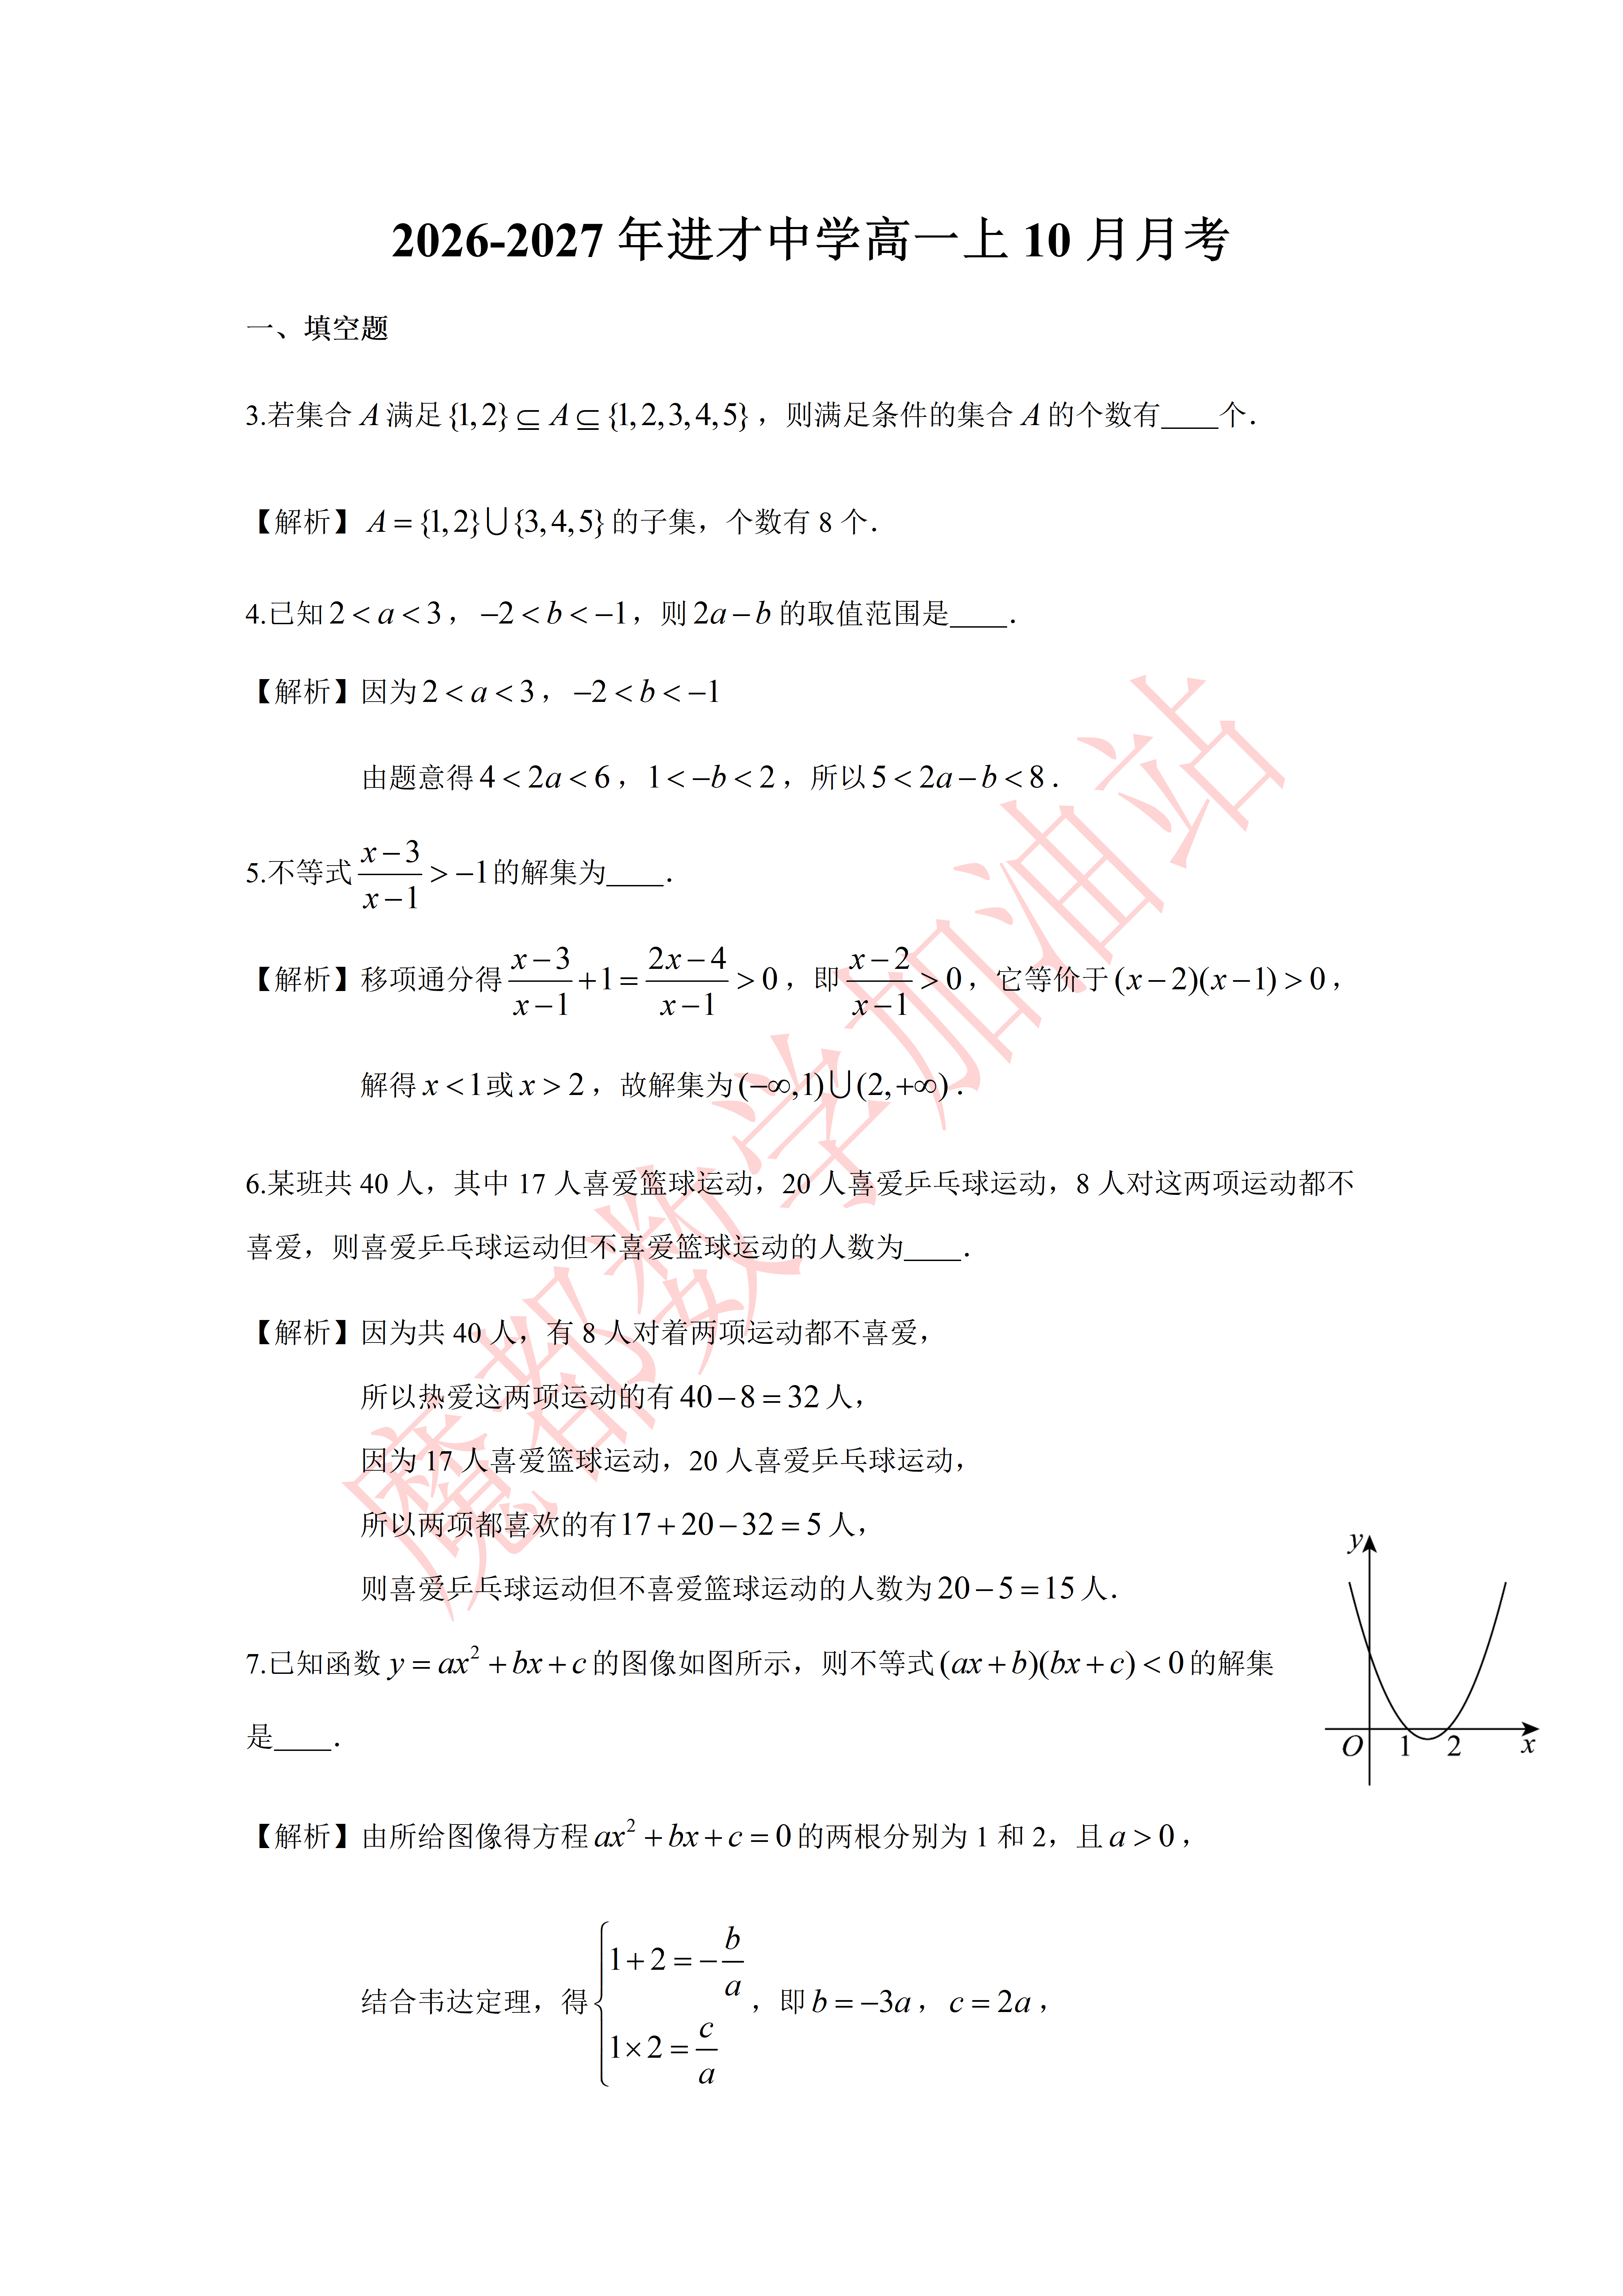
\includegraphics[width=.22\linewidth,trim=3879bp 1490bp 238bp 4492bp,clip]{../原图/高一60_进才中学_10月月考/01.png}
\end{center}

\ifanswer
\solbegin
\step{由所给图像得方程 $ax^2+bx+c=0$ 的两根分别为 1 和 2，且 $a>0$，}
\step{结合韦达定理，得 $\begin{cases}1+2=-\dfrac ba\\ 1\times2=\dfrac ca\end{cases}$，即 $b=-3a$，$c=2a$，}
\step{所以不等式 $(ax+b)(bx+c)<0$ 即 $(ax-3a)(-3ax+2a)<0$，}
\step{化简得 $(x-3)(3x-2)>0$，解得 $x<\dfrac23$ 或 $x>3$，}
\step{所以不等式 $(ax+b)(bx+c)<0$ 的解集是 $(-\infty,\dfrac23)\cup(3,+\infty)$.}
\solend
\fi

\item 已知集合 $A=\{x\mid ax=6\}$，满足 $A\subseteq\Z$，则整数 $a$ 的所有可能取值有\blankline[4.4em]个.

\ifanswer
\solbegin
\step{当 $a=0$ 时，$A=\varnothing$，而 $\varnothing\subseteq\Z$，满足题意，}
\step{当 $a\neq0$ 时，$A=\left\{\dfrac6a\right\}$，要使 $A\subseteq\Z$，则 $\dfrac6a\in\Z$，所以 $a=\pm1,\pm2,\pm3,\pm6$，}
\step{综上，整数 $a$ 的可能取值为 0，$\pm1$，$\pm2$，$\pm3$，$\pm6$，共 9 个.}
\solend
\fi

\item 设关于 $x$ 的方程 $x^2+kx+n=0$ 有两个不同实根 $x_1$、$x_2$，且 $\dfrac1{x_1}+\dfrac1{x_2}=2$，则实数 $n$ 的取值范围是\blankline[4.4em].

\ifanswer
\solbegin
\step{由于方程 $x^2+kx+n=0$ 有两个不同实根 $x_1$、$x_2$，}
\step{因此 $\Delta=k^2-4n>0$，$x_1+x_2=-k$，$x_1x_2=n$，}
\step{由 $\dfrac1{x_1}+\dfrac1{x_2}=\dfrac{x_1+x_2}{x_1x_2}=\dfrac{-k}{n}=2$，得 $k=-2n$，}
\step{因此 $\Delta=k^2-4n=4n^2-4n>0$，解得 $n<0$ 或 $n>1$，}
\step{则实数 $n$ 的取值范围是 $(-\infty,0)\cup(1,+\infty)$.}
\solend
\fi

\item 某船从甲地沿河顺流航行 $75\mathrm{km}$，到达乙码头，停留 $30\mathrm{min}$ 后再逆流航行 $126\mathrm{km}$ 到达丙地，若水流速度为 $4\mathrm{km/h}$，且该船要在 $5\mathrm{h}$ 内完成航行任务，那么船的速度至少达到\blankline[4.4em]$\mathrm{km/h}$.

\ifanswer
\solbegin
\step{设该轮船在静水中的速度是 $x$ 千米/小时，水流速度是 4 千米/小时，}
\step{由题意得 $\dfrac{75}{4+x}+0.5+\dfrac{126}{x-4}\leqslant5$，即 $9x^2-402x-552\geqslant0$，解得 $x\geqslant46$，}
\step{答：该船的速度至少是 46 千米/小时.}
\solend
\fi

\item 设实数 $a,b,c$ 满足 $a^2+b^2\leqslant c<1$，则 $a+\dfrac12b+c$ 的最小值为\blankline[4.4em].

\ifanswer
\solbegin
\step{因为 $c\geqslant a^2+b^2$，}
\step{所以 $a+\dfrac12b+c\geqslant a+\dfrac12b+a^2+b^2=\left(a+\dfrac12\right)^2+\left(b+\dfrac14\right)^2-\dfrac5{16}\geqslant-\dfrac5{16}$，}
\step{当 $a=-\dfrac12,b=-\dfrac14,c=a^2+b^2=\dfrac5{16}$（此时 $c<1$ 成立）时取到等号，}
\step{故最小值为 $-\dfrac5{16}$.}
\solend
\fi

\item 已知集合 $A=\{x\in\N^*\mid1\leqslant x\leqslant2026\}$. 设集合 $B=\{b_1,b_2,b_3,\cdots,b_n\}$ 满足 $B\subseteq A$，且对任意的 $b_i$、$b_j$、$b_k\in B(i$、$j$、$k\in\{1,2,3,\cdots,n\})$，存在 $m\in\N^*$，使得 $b_i+b_j+b_k=39m$，则 $n$ 的最大值为\blankline[4.4em].

\ifanswer
\solbegin
\step{因为 $39=1\times39=3\times13$，所以 $n$ 的最大值大于 3，}
\step{若对任意的 $b_i$、$b_j$、$b_k\in B$，存在 $m\in\N^*$，使得 $b_i+b_j+b_k=39m$，}
\step{则集合 $B$ 的元素除以 39 的余数均为 0 或均为 13 或均为 26，}
\step{即 $B=\{39,78,\cdots,39n\}$ 或 $B=\{13,52,\cdots,39n-26\}$}
\step{或 $B=\{26,65,\cdots,39n-13\}$，}
\step{若 $B=\{39,78,\cdots,39n\}$，则 $39n\leqslant2026$，}
\step{解得 $n\leqslant\dfrac{2026}{39}\in(51,52)$，此时 $n$ 的最大值为 51；}
\step{若 $B=\{13,52,\cdots,39n-26\}$，则 $39n-26\leqslant2026$，}
\step{解得 $n\leqslant\dfrac{684}{13}\in(52,53)$，此时 $n$ 的最大值为 52；}
\step{若 $B=\{26,65,\cdots,39n-13\}$，则 $39n-13\leqslant2026$，}
\step{解得 $n\leqslant\dfrac{2039}{39}\in(52,53)$，此时 $n$ 的最大值为 52；}
\step{综上，$n$ 的最大值为 52.}
\solend
\fi

\end{enumerate}

\bigsec{二、选择题}

\begin{enumerate}
\setcounter{enumi}{12}

% 第 13 题原卷无【答案】/【解析】段，答案“B”直接印在题干括号内，
% 按 高一53 第 13 题的成例括号留空、答案另提为 \ans{}（见文件头）
\item 已知 $a$、$b\in\R$，则“$|a|>|b|$”是“$a>|b|$”的\mbox{（\quad）}

\keepwithprev
A. 充分不必要条件\qquad B. 必要不充分条件

C. 充要条件\qquad D. 既不充分也不必要条件

\ifanswer
\ans{$B$}
\fi

\item 如果关于 $x$ 的一元二次方程 $x^2+2mx+(m+2)=0$ 有一正根一负根，那么 $m$ 的取值范围为\mbox{（\quad）}

\keepwithprev
A. $(-2,-1)$\qquad B. $(-1,2)$

C. $(-\infty,-1)\cup(2,+\infty)$\qquad D. $(-\infty,-2)$

\ifanswer
\solbegin
\step{设两根为 $x_1,x_2$，方程有一正根一负根，则 $\begin{cases}x_1x_2=m+2<0\\ \Delta=4m^2-4(m+2)>0\end{cases}$，}
\step{解得 $m<-2$，故选 $D$.}
\solend
\fi

\item 若不等式 $|3x-a|\leqslant x+2$ 的解集包含集合 $[0,1]$，则实数 $a$ 的取值范围为\mbox{（\quad）}

\keepwithprev
A. $[0,2]$\qquad B. $[0,1]$

C. $[1,2]$\qquad D. $(1,2)$

\ifanswer
\solbegin
% 原卷“法一：”“法二：”排红色加粗（全卷唯一红字），本稿按全稿子题标号样式排 \stepm
% （详见文件头“与原卷的排版差异”⑦）
\stepm{法一：}{不等式 $|3x-a|\leqslant x+2$ 化为 $2x-2\leqslant a\leqslant4x+2$，}
% 原卷此句缺动词（疑漏“对”字），照录未改（见文件头“原卷存疑”④）
\step{$[0,1]$ 使 $2x-2\leqslant a\leqslant4x+2$ 成立，则 $0\leqslant a\leqslant2$，故选 $A$.}
\stepm{法二：}{将两边平方整理得 $8x^2-(6a+4)x+a^2-4\leqslant0$ 对 $[0,1]$ 恒成立，}
\step{则有 $\begin{cases}a^2-4\leqslant0\\ a^2-6a\leqslant0\end{cases}$，解得 $0\leqslant a\leqslant2$，故选 $A$.}
\solend
\fi

\item 数学组 Y 老师在白纸上写下以下四个命题：

①这四个命题中至少有一个是真的；②这四个命题中至少有两个是真的；

③这四个命题中至少有两个是假的；④这四个命题中至少有一个是假的；

每个命题非真即假. 问 Y 老师在纸上写的假命题有几个？\mbox{（\quad）}

\keepwithprev
A. 0\qquad B. 1

C. 2\qquad D. 3

\ifanswer
\solbegin
\step{设四个命题中真命题的个数为 $t$，则①真 $\iff t\geqslant1$，②真 $\iff t\geqslant2$，}
\step{③真 $\iff t\leqslant2$，④真 $\iff t\leqslant3$.}
\step{逐一检验：$t=0$ 时③④为真，应为 $t=2$，矛盾；}
\step{$t=1$ 时①③④为真，应为 $t=3$，矛盾；}
\step{$t=2$ 时四个命题全为真，应为 $t=4$，矛盾；}
\step{$t=3$ 时①②④为真、③为假，恰有 3 个真命题，符合；}
\step{$t=4$ 时①②为真，应为 $t=2$，矛盾.}
\step{所以恰有 1 个假命题，故选 $B$.}
\solend
\fi

\end{enumerate}

\bigsec{三、解答题}

\begin{enumerate}
\setcounter{enumi}{16}

\item 已知：$x\in\R$，$a=x^2-1$，$b=4x+5$. 求证：$a$、$b$ 中至少有一个大于等于 0.

\ifanswer
\solbegin
\step{假设 $a$、$b$ 都小于 0，即 $a<0$，$b<0$，则 $a+b<0$.}
\step{又 $a+b=x^2-1+4x+5=x^2+4x+4=(x+2)^2\geqslant0$，}
\step{这与假设所得 $a+b<0$ 矛盾，故假设不成立，}
\step{所以 $a$、$b$ 中至少有一个大于等于 0.}
\solend
\fi

\ansspace[6]

% 原卷 A、B 两个集合定义之间排半角逗号“,”（5 倍放大核，右侧字距 19px，与全卷全角“，”的 65—79px 字距判然有别）；
% 本稿原误抄为全角“，”——已照录原卷半角（见文件头“与原卷的排版差异”⑤）
\item 已知集合 $A=\{x\mid4\leqslant x\leqslant12\}$,$B=\{x\mid a\leqslant x\leqslant2a+1\}$.

（1）若 $a=2$，求 $\overline A\cap B$；

（2）已知 $A\cup B=A$，求实数 $a$ 的取值范围.

\ifanswer
\solbegin
\stepm{(1)}{当 $a=2$ 时，$B=\{x\mid2\leqslant x\leqslant5\}$，}
\step{而 $A=\{x\mid4\leqslant x\leqslant12\}$，则 $\overline A=(-\infty,4)\cup(12,+\infty)$，所以 $\overline A\cap B=[2,4)$.}
\stepm{(2)}{$A\cup B=A$ 即 $B\subseteq A$.}
\stepm{①}{当 $B=\varnothing$ 时，$a>2a+1$，即 $a<-1$，符合；}
\stepm{②}{当 $B\neq\varnothing$ 时，需 $a\leqslant2a+1$ 且 $a\geqslant4$ 且 $2a+1\leqslant12$，即 $4\leqslant a\leqslant\dfrac{11}2$.}
\step{综上，$a$ 的取值范围是 $(-\infty,-1)\cup\left[4,\dfrac{11}2\right]$.}
\solend
\fi

\ansspace[8]

\item （1）若关于 $x$ 的不等式 $ax^2-3x+2<0$ 的解集不是空集，求实数 $a$ 的取值范围；

（2）求关于 $x$ 的不等式 $ax^2-3x+2>ax-1$ 的解集.

\ifanswer
\solbegin
\stepm{(1)}{若 $a>0$，关于 $x$ 的不等式 $ax^2-3x+2<0$ 的解集不空，}
\step{所以一元二次方程 $ax^2-3x+2=0$ 的判别式大于零，}
\step{即 $(-3)^2-8a>0\Rightarrow a<\dfrac98$，结合 $a>0$ 得 $0<a<\dfrac98$；}
\step{若 $a\leqslant0$，则关于 $x$ 的不等式 $ax^2-3x+2<0$ 的解集不是空集；}
\step{综上，实数 $a$ 的取值范围是 $\left(-\infty,\dfrac98\right)$.}
\stepm{(2)}{$ax^2-3x+2>ax-1\Rightarrow ax^2-(a+3)x+3>0\Rightarrow(ax-3)(x-1)>0$，}
\step{当 $a=0$ 时，不等式为 $x-1<0$，不等式的解集为 $\{x\mid x<1\}$；}
\step{当 $a<0$ 时，不等式化为 $\left(x-\dfrac3a\right)(x-1)<0$，}
\step{不等式的解集为 $\left\{x\mid\dfrac3a<x<1\right\}$，}
\step{当 $a>0$ 时，方程 $ax^2-3x+2=ax-1$ 的两个根分别为：$\dfrac3a,1$.}
\step{当 $a=3$ 时，两根相等，故不等式的解集为 $\{x\mid x\neq1\}$；}
\step{当 $a>3$ 时，$\dfrac3a<1$，不等式的解集为 $\left\{x\mid x<\dfrac3a\right.$ 或 $\left.x>1\right\}$；}
\step{当 $0<a<3$ 时，$\dfrac3a>1$，不等式的解集为 $\left\{x\mid x<1\right.$ 或 $\left.x>\dfrac3a\right\}$；}
\step{综上所述，当 $a<0$ 时，不等式的解集为 $\left\{x\mid\dfrac3a<x<1\right\}$，}
\step{当 $a=0$ 时，不等式的解集为 $\{x\mid x<1\}$，}
\step{当 $0<a<3$ 时，不等式的解集为 $\left\{x\mid x<1\right.$ 或 $\left.x>\dfrac3a\right\}$，}
\step{当 $a=3$ 时，不等式的解集为 $\{x\mid x\neq1\}$，}
\step{当 $a>3$ 时，不等式的解集为 $\left\{x\mid x<\dfrac3a\right.$ 或 $\left.x>1\right\}$.}
\solend
\fi

\ansspace[8]

\item 设命题 $p$：对任意 $x\in\R$，使得不等式 $mx^2-mx+2>0$ 恒成立；命题 $q$：存在 $0\leqslant x\leqslant3$，不等式 $2x-2\geqslant|m|$ 成立.

（1）若 $p$ 为真命题，求实数 $m$ 的取值范围；

（2）若 $p$、$q$ 有且只有一个是真命题，求实数 $m$ 的取值范围.

\ifanswer
\solbegin
\stepm{(1)}{因为 $p:\forall x\in\R$，$mx^2-mx+2>0$ 为真命题，}
\step{所以当 $m=0$ 时，不等式为 $2>0$，在 $\R$ 上恒成立，符合题意；}
\step{当 $m\neq0$ 时，$\begin{cases}m>0\\ \Delta=m^2-8m<0\end{cases}$，解得 $0<m<8$.}
\step{综上，实数 $m$ 的取值范围为 $[0,8)$.}
\stepm{(2)}{若 $q$ 为真命题，即 $q:\exists0\leqslant x\leqslant3$，$2x-2\geqslant|m|$，}
\step{则对于 $0\leqslant x\leqslant3$，$(2x-2)_{max}\geqslant|m|$.}
\step{由于 $0\leqslant x\leqslant3$，$2x-2\in[-2,4]$，所以 $|m|\leqslant4$，解得 $-4\leqslant m\leqslant4$，}
\step{又因为 $p$、$q$ 有且只有一个是真命题，}
\step{所以当 $p$ 真 $q$ 假时，$\begin{cases}0\leqslant m<8\\ m<-4\text{或}m>4\end{cases}$，解得 $4<m<8$；}
\step{当 $p$ 假 $q$ 真时，$\begin{cases}m<0\text{或}m\geqslant8\\ -4\leqslant m\leqslant4\end{cases}$，解得 $-4\leqslant m<0$；}
\step{综上，实数 $m$ 的取值范围为 $[-4,0)\cup(4,8)$.}
\solend
\fi

\ansspace[10]

\item 已知集合 $A=\{a_1,a_2,\cdots,a_k\}(k\geqslant2)$. 其中 $a_i\in\N^*(i=1,2,\cdots,k)$. 若对于任意的 $a\in A$，总有 $\dfrac1a\notin A$，则称集合 $A$ 具有性质 $P$. 由 $A$ 中的元素构成两个相应的集合：$S=\{(a,b)\mid a\in A,b\in A,ab\in A\}$，$T=\left\{(a,b)\mid a\in A,b\in A,\dfrac ab\in A\right\}$，其中 $(a,b)$ 是有序数对，集合 $S$ 和 $T$ 中的元素个数分别为 $m$ 和 $n$.

（1）检验集合 $\{2,3,6\}$ 与 $\{1,2,4\}$ 是否具有性质 $P$，并对其中具有性质 $P$ 的集合，写出相应的集合 $S$ 和 $T$；

（2）对任何具有性质 $P$ 的集合 $A$，$n$ 的最大值为多少？（直接写出答案，无需说明理由）；

% 原卷题干的小问编号跳号：印作 (1)(2)(4)，本稿照录 (4)、未改成 (3)（见文件头“原卷存疑”①）
（4）判断 $m$ 和 $n$ 的大小关系，并证明你的结论.

\ifanswer
\solbegin
\stepm{(1)}{因为 $\dfrac12\in\{1,2,4\}$，所以 $\{1,2,4\}$ 不具有性质 $P$；}
\step{因为 $\dfrac12\notin\{2,3,6\}$，$\dfrac13\notin\{2,3,6\}$，$\dfrac16\notin\{2,3,6\}$，所以 $\{2,3,6\}$ 具有性质 $P$.}
\step{$S=\{(2,3),(3,2)\}$，$T=\{(6,2),(6,3)\}$；}
\stepm{(2)}{因为对于任意的 $a\in A$，总有 $\dfrac1a\notin A$，所以 $1\notin A$，}
% 原卷此处印作“$\{(a_i,a_i)\}\in T$”，与上一句“$1\notin A$”及下文“最多为 $C_k^2$”的推理
% 均不自洽（应为“$\notin$”），已 8 倍放大确认无斜线；照录未改（见文件头“原卷存疑”③）
\step{从而 $\{(a_i,a_i)\}\in T(i=1,2,\cdots,k)$.}
\step{因为 $a\in A,b\in A,\dfrac ab\in A$，所以当 $i\neq j$ 时，}
\step{$(a_i,a_j)\in T$ 和 $(a_j,a_i)\in T(i,j=1,2,\cdots,k)$ 至多有一个成立，}
\step{所以集合 $T$ 中的元素个数最多为 $C_k^2=\dfrac{k(k-1)}2$，即 $n\leqslant\dfrac{k(k-1)}2$.}
% 原卷【解析】把第 (4) 问标作“(3)”（与题干跳号相应），本稿照录未改（见文件头“原卷存疑”①）
\stepm{(3)}{$m=n$，证明如下：}
\step{①设 $(a,b)\in T$，则 $a\in A,b\in A,\dfrac ab\in A$. 设 $c=\dfrac ab$，则 $a=bc$，}
\step{故 $b\in A$，$c\in A$，$bc\in A$，从而 $(b,c)\in S$，}
\step{即对 $\forall(a,b)\in T$，总 $\exists c$ 使 $(b,c)\in S$，从而 $n\leqslant m$.}
\step{②设 $(p,q)\in S$，则 $p\in A$，$q\in A$，$pq\in A$.}
\step{设 $r=pq$，则 $q=\dfrac rp$，故 $r\in A,p\in A,\dfrac rp\in A$，从而 $(r,p)\in T$，}
\step{即对 $\forall(p,q)\in S$，总 $\exists r$ 使 $(r,p)\in T$，从而 $m\leqslant n$.}
\step{由①②得 $m=n$.}
\solend
\fi

\ansspace*[10]

\end{enumerate}

\end{document}
"
% 紧凑版：xelatex "\def\iscompact{1}% 高一60_进才中学_10月月考.tex
%   —— 高一上数学“2026-2027 年进才中学高一上 10 月月考”（讲评版）
% 试卷版：xelatex 高一60_进才中学_10月月考.tex
% 答案版：xelatex "\def\isanswer{1}\input{高一60_进才中学_10月月考.tex}"
% 紧凑版：xelatex "\def\iscompact{1}\input{高一60_进才中学_10月月考.tex}"
%
% 原文链接：https://mp.weixin.qq.com/s/2ZLKB3IONEDhcUAfAAYE2A。
% 公众号“魔都数学加油站”作者破晓于 2026-10-14 22:15 发布。
% 原图 9 张（`原图/高一60_进才中学_10月月考/01..09.png`）：第 1—8 页 4762×6735，
% 第 9 页 2560×3620（同一篇内两档分辨率）。
%
% 卷首标题：照卷面印作“2026--2027 年进才中学高一上 10 月月考”（公众号标题中的“上海市”
% 卷面标题行没有，本稿照卷面），年份区间按全稿惯例排 en dash。原卷只有一行标题、无副标题。
%
% 篇幅与题号：原卷自第 3 题起编号（第 1、2 题不在本卷内）。填空题 3—12（10 题）、
% 选择题 13—16（4 题）、解答题 17—21（5 题），共 19 题。本稿沿用原节与原题号，
% 只改排为全稿统一的大节样式（原卷小节标题为“一、填空题”“二、选择题”“三、解答题”）。
%
% 讲评版：原卷每题下直接印【答案】或【解析】。**只印【解析】的 18 题**，本稿按全稿口径
% 收进答案版、不另提 \ans{}——第 14、15、16 题的结论写在解析末句（“故选 D／A／B”），
% 亦照录在解析内。**第 13 题原卷没有任何【答案】/【解析】段**，答案“B”直接印在题干括号内
% （“（ B ）”），本稿按 高一53 第 13 题的成例把括号留空、答案另提为 \ans{$B$}（见下）。
%
% 副标题：原卷未印副标题。本稿按“知识模块”口径标作“集合与常用逻辑用语、不等式”：
% 19 题中集合与常用逻辑用语 10 题（第 3、6、8、12、13、16、17、18、20、21 题，
% 含子集计数、韦恩图容斥、集合运算、命题与充要条件、反证法、新定义），
% 不等式 9 题（含不等式性质、分式不等式、二次函数与解集、韦达定理与判别式、
% 不等式应用、最值、根的分布、绝对值不等式恒成立、含参二次不等式：第 4、5、7、9、10、
% 11、14、15、19 题），两类均远超三分之一，故并标。口径同 高一46、高一47、高一48、
% 高一51—高一59。
%
% 与原卷的排版差异：
%   ① 原卷每题下直接印【答案】/【解析】，本稿按全稿惯例将答案与解析置于答案版，试卷版保持干净；
%   ② 原卷未印副标题，本稿按“知识模块”口径补出；
%   ③ 原卷填空横线约两个字宽，本稿按全稿惯例统一排 \blankline[4.4em]；
%   ④ 原卷实数集排斜体 $R$（第 13、17、20 题）、正整数集排 $N^*$（第 12、21 题）、
%      整数集排粗体 $\mathbf{Z}$（第 8 题），本稿按全稿惯例改用 $\R$、$\N^*$、$\Z$；
%      空集记号统一为 \varnothing；
%   ⑤ 原卷在数学式内多处用半角逗号（如 $x_1,x_2$、$a,b\in R$，以及第 18 题题干
%      $A=\{x\mid4\leqslant x\leqslant12\}$,$B=\{x\mid a\leqslant x\leqslant2a+1\}$ 之间的逗号），
%      均照录未强改（第 18 题题干那一处本稿首轮曾误作全角“，”，第二轮已订正）；
%      句末句点按全稿惯例排西文句点；
%   ⑥ 第 13 题印在题干括号内的答案“B”移入 \ans{}，见上；
%   ⑦ 第 15 题【解析】的“法一：”“法二：”标号原卷排**红色加粗**（全卷唯一的红字，2 处），
%      本稿按全稿子题标号样式排 \stepm{法一：}{…}、\stepm{法二：}{…}（加粗着色、不改黑色
%      基调），冒号照原卷排全角；
%   ⑧ 第 7 题的图像原卷排在题干右侧（与题干第 1 行同高），本稿居中排在题干之后；
%      图自原图第 01 页裁切（trim），不另存图片文件；
%   ⑨ 原卷第 10 题的长度与速度单位原卷排斜体（$75km$、$4km/h$ 等），本稿按全稿惯例
%      改排正体 $\mathrm{km}$、$\mathrm{km/h}$（同 高一56 第 13 题）；每道解答题原卷未留
%      作答空白，本稿按全稿惯例加 \ansspace。
%
% 原卷存疑（照录未改，见源码中该处上方注释）：
%   ① 第 21 题题干的小问编号**跳号**：印作 (1)(2)(4)，而紧随其后的【解析】按 (1)(2)(3) 写
%      —— 题干第 (4) 问实为第 (3) 问。本稿题干照录 (1)(2)(4)、解析照录 (3)，未改
%      （与 高一22 第 16 题“解析误标 (2)”同一处理）。
%   ② 第 6 题【解析】“有 8 人**对着**两项运动都不喜爱”，“对着”疑为“对这”之误，照录未改。
%   ③ 第 21(2) 题【解析】首行“所以 $1\notin A$，从而 $\{(a_i,a_i)\}\in T(i=1,2,\cdots,k)$”
%      —— 由 $1\notin A$ 应得 $(a_i,a_i)\notin T$（因 $a_i/a_i=1$），与紧随的“$T$ 中元素
%      个数最多为 $C_k^2$”这一推理亦只有“$\notin$”才自洽；原卷此处印作“$\in$”，
%      已 8 倍放大确认无斜线。**照录原卷的 $\in$、未改**。
%   ④ 第 15 题【解析】法一“$[0,1]$ 使 $2x-2\leqslant a\leqslant4x+2$ 成立”一句缺动词
%      （疑漏“对”字），照录未改。
%
\documentclass[a4paper,11pt]{article}
\usepackage{common}

\begin{document}

\examtitlest[3]{2026--2027 年进才中学高一上 10 月月考}{集合与常用逻辑用语、不等式}

\bigsec{一、填空题}

\begin{enumerate}
\setcounter{enumi}{2}

\item 若集合 $A$ 满足 $\{1,2\}\subseteq A\subseteq\{1,2,3,4,5\}$，则满足条件的集合 $A$ 的个数有\blankline[4.4em]个.

\ifanswer
\solbegin
\step{$A=\{1,2\}\cup\{3,4,5\}$ 的子集，个数有 8 个.}
\solend
\fi

\item 已知 $2<a<3$，$-2<b<-1$，则 $2a-b$ 的取值范围是\blankline[4.4em].

\ifanswer
\solbegin
\step{因为 $2<a<3$，$-2<b<-1$，}
\step{由题意得 $4<2a<6$，$1<-b<2$，所以 $5<2a-b<8$.}
\solend
\fi

\item 不等式 $\dfrac{x-3}{x-1}>-1$ 的解集为\blankline[4.4em].

\ifanswer
\solbegin
\step{移项通分得 $\dfrac{x-3}{x-1}+1=\dfrac{2x-4}{x-1}>0$，即 $\dfrac{x-2}{x-1}>0$，它等价于 $(x-2)(x-1)>0$，}
\step{解得 $x<1$ 或 $x>2$，故解集为 $(-\infty,1)\cup(2,+\infty)$.}
\solend
\fi

\item 某班共 40 人，其中 17 人喜爱篮球运动，20 人喜爱乒乓球运动，8 人对这两项运动都不喜爱，则喜爱乒乓球运动但不喜爱篮球运动的人数为\blankline[4.4em].

\ifanswer
\solbegin
% 原卷作“对着两项运动都不喜爱”（疑为“对这”之误），照录未改（见文件头“原卷存疑”②）
\step{因为共 40 人，有 8 人对着两项运动都不喜爱，}
\step{所以热爱这两项运动的有 $40-8=32$ 人，}
\step{因为 17 人喜爱篮球运动，20 人喜爱乒乓球运动，}
\step{所以两项都喜欢的有 $17+20-32=5$ 人，}
\step{则喜爱乒乓球运动但不喜爱篮球运动的人数为 $20-5=15$ 人.}
\solend
\fi

\item 已知函数 $y=ax^2+bx+c$ 的图像如图所示，则不等式 $(ax+b)(bx+c)<0$ 的解集是\blankline[4.4em].

% 原图第 01 页题干右侧的图像直接裁取。裁框取图外框 x 3887–4516、y 4500–5237
% （四周各留约 8px），trim=左 3879bp／下 1490bp／右 238bp／上 4492bp
% （页宽 4762、页高 6735）。
\begin{center}
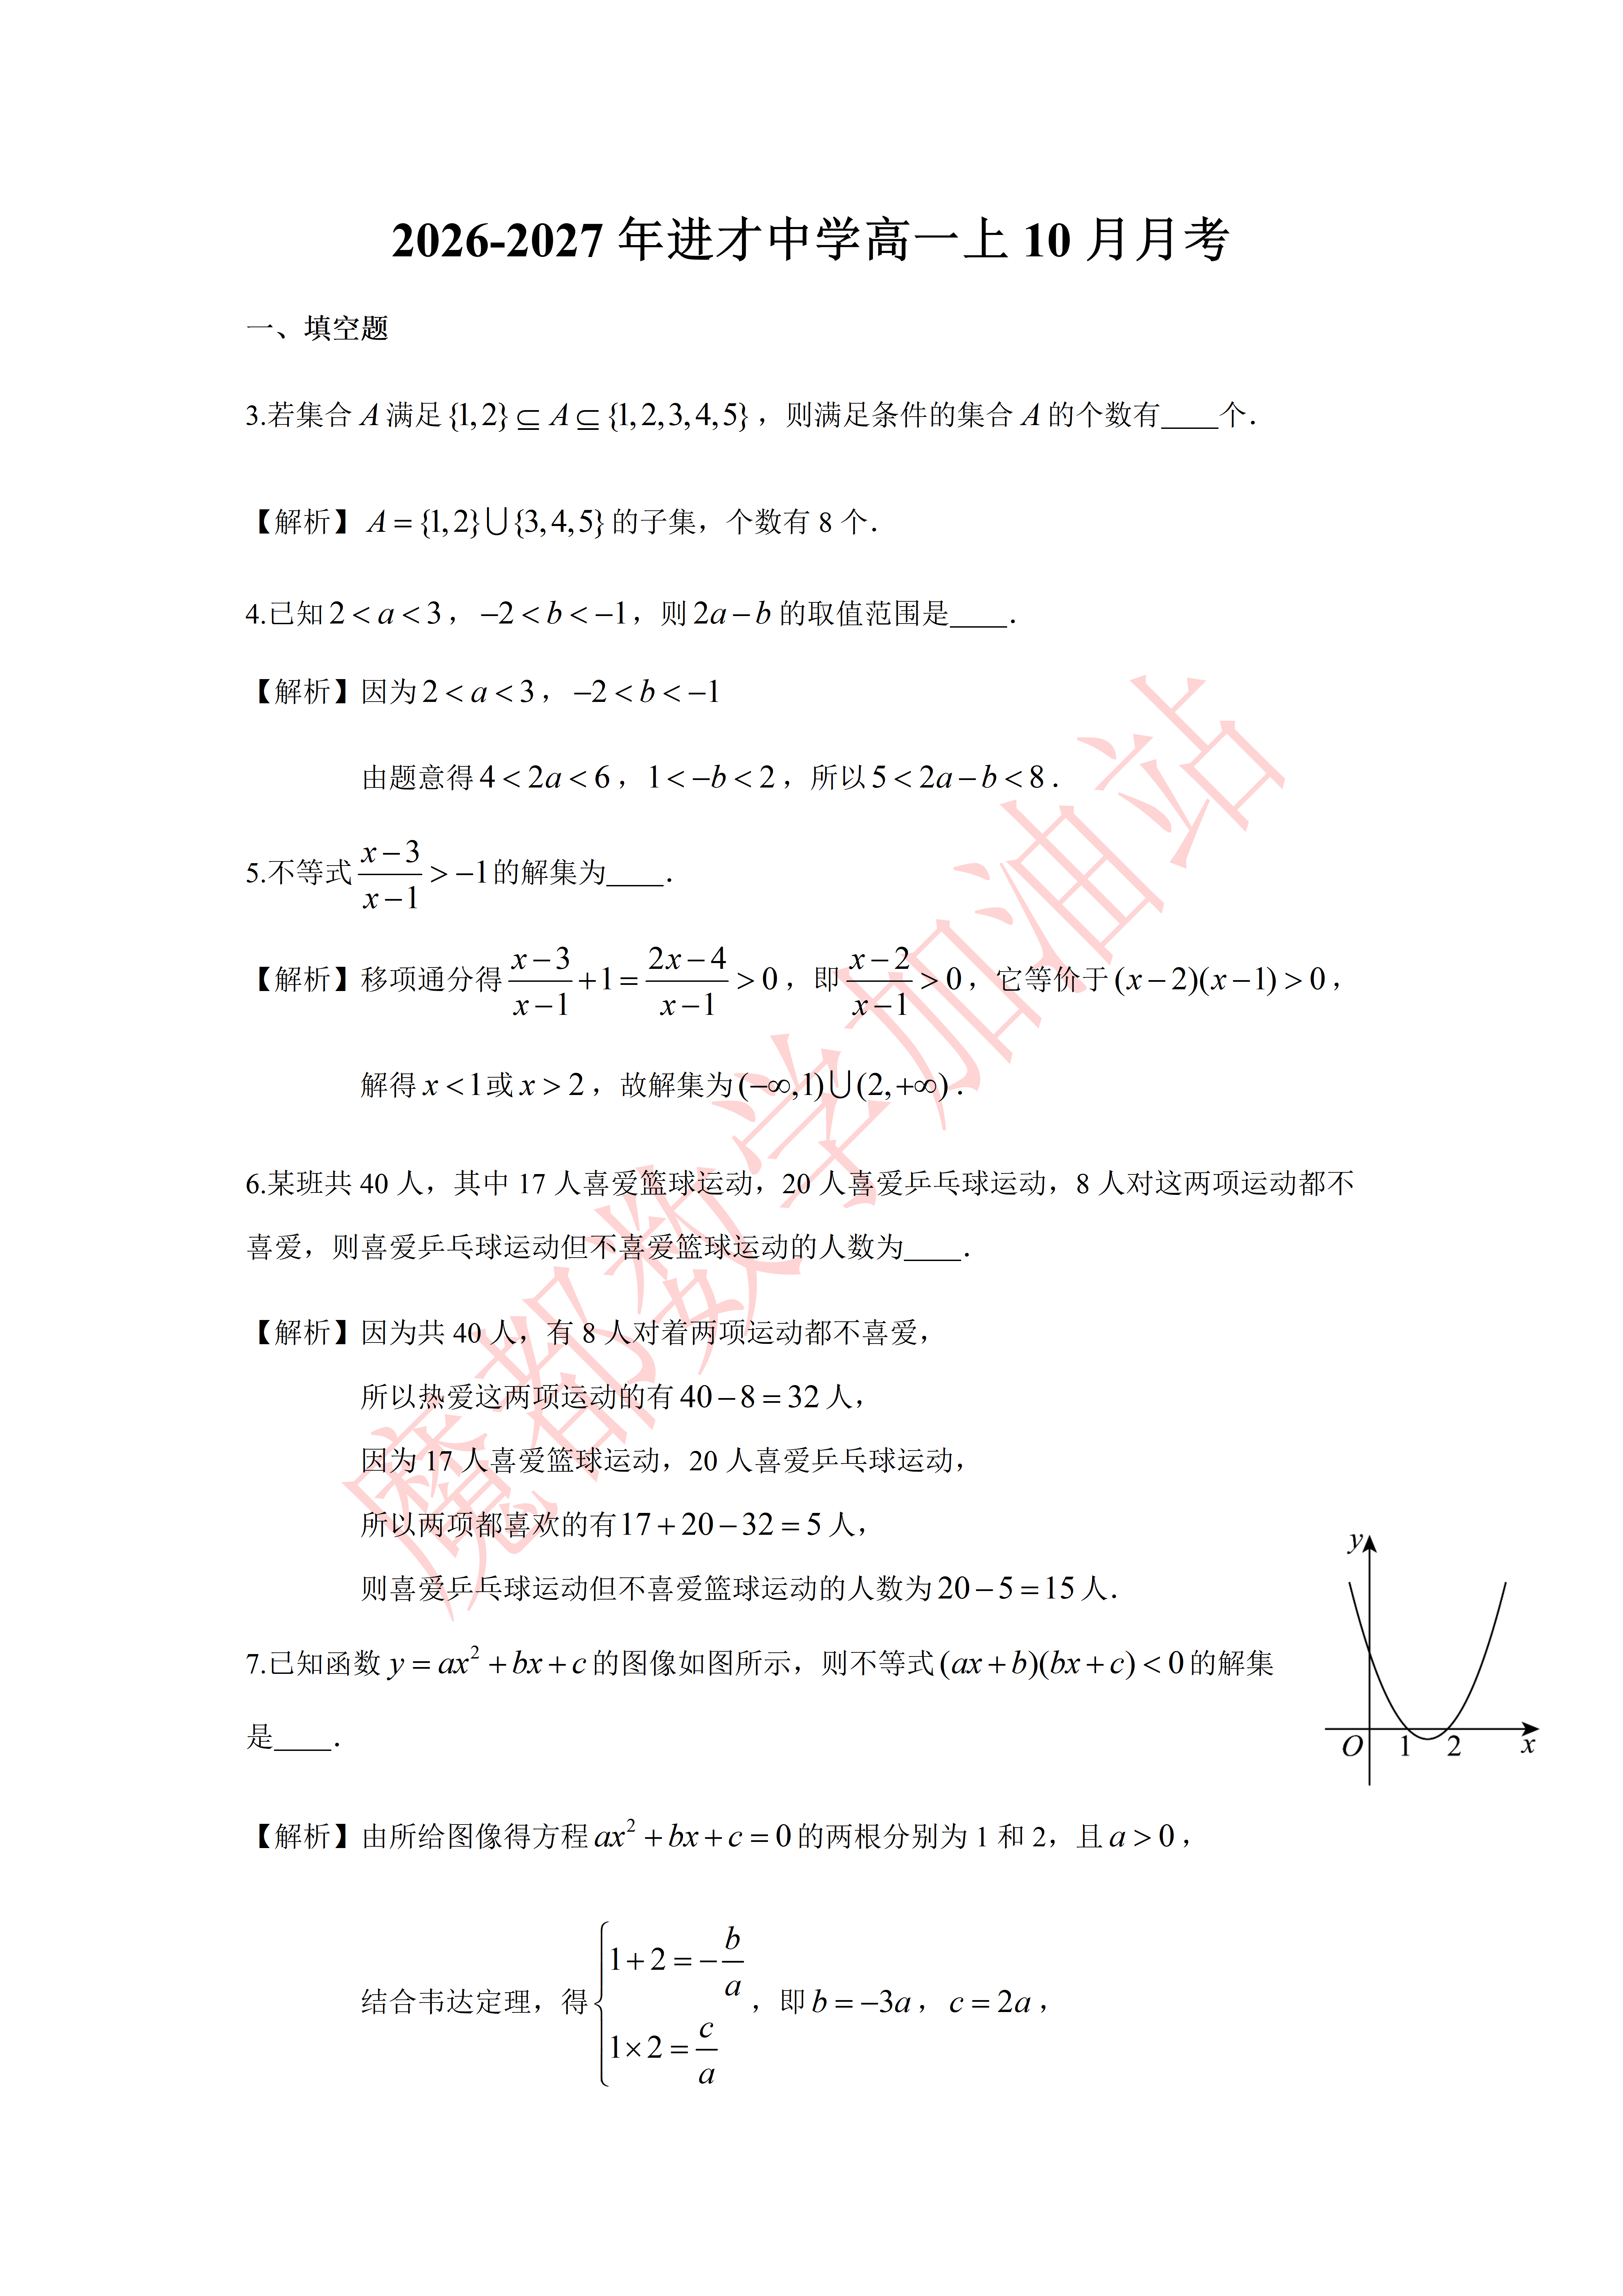
\includegraphics[width=.22\linewidth,trim=3879bp 1490bp 238bp 4492bp,clip]{../原图/高一60_进才中学_10月月考/01.png}
\end{center}

\ifanswer
\solbegin
\step{由所给图像得方程 $ax^2+bx+c=0$ 的两根分别为 1 和 2，且 $a>0$，}
\step{结合韦达定理，得 $\begin{cases}1+2=-\dfrac ba\\ 1\times2=\dfrac ca\end{cases}$，即 $b=-3a$，$c=2a$，}
\step{所以不等式 $(ax+b)(bx+c)<0$ 即 $(ax-3a)(-3ax+2a)<0$，}
\step{化简得 $(x-3)(3x-2)>0$，解得 $x<\dfrac23$ 或 $x>3$，}
\step{所以不等式 $(ax+b)(bx+c)<0$ 的解集是 $(-\infty,\dfrac23)\cup(3,+\infty)$.}
\solend
\fi

\item 已知集合 $A=\{x\mid ax=6\}$，满足 $A\subseteq\Z$，则整数 $a$ 的所有可能取值有\blankline[4.4em]个.

\ifanswer
\solbegin
\step{当 $a=0$ 时，$A=\varnothing$，而 $\varnothing\subseteq\Z$，满足题意，}
\step{当 $a\neq0$ 时，$A=\left\{\dfrac6a\right\}$，要使 $A\subseteq\Z$，则 $\dfrac6a\in\Z$，所以 $a=\pm1,\pm2,\pm3,\pm6$，}
\step{综上，整数 $a$ 的可能取值为 0，$\pm1$，$\pm2$，$\pm3$，$\pm6$，共 9 个.}
\solend
\fi

\item 设关于 $x$ 的方程 $x^2+kx+n=0$ 有两个不同实根 $x_1$、$x_2$，且 $\dfrac1{x_1}+\dfrac1{x_2}=2$，则实数 $n$ 的取值范围是\blankline[4.4em].

\ifanswer
\solbegin
\step{由于方程 $x^2+kx+n=0$ 有两个不同实根 $x_1$、$x_2$，}
\step{因此 $\Delta=k^2-4n>0$，$x_1+x_2=-k$，$x_1x_2=n$，}
\step{由 $\dfrac1{x_1}+\dfrac1{x_2}=\dfrac{x_1+x_2}{x_1x_2}=\dfrac{-k}{n}=2$，得 $k=-2n$，}
\step{因此 $\Delta=k^2-4n=4n^2-4n>0$，解得 $n<0$ 或 $n>1$，}
\step{则实数 $n$ 的取值范围是 $(-\infty,0)\cup(1,+\infty)$.}
\solend
\fi

\item 某船从甲地沿河顺流航行 $75\mathrm{km}$，到达乙码头，停留 $30\mathrm{min}$ 后再逆流航行 $126\mathrm{km}$ 到达丙地，若水流速度为 $4\mathrm{km/h}$，且该船要在 $5\mathrm{h}$ 内完成航行任务，那么船的速度至少达到\blankline[4.4em]$\mathrm{km/h}$.

\ifanswer
\solbegin
\step{设该轮船在静水中的速度是 $x$ 千米/小时，水流速度是 4 千米/小时，}
\step{由题意得 $\dfrac{75}{4+x}+0.5+\dfrac{126}{x-4}\leqslant5$，即 $9x^2-402x-552\geqslant0$，解得 $x\geqslant46$，}
\step{答：该船的速度至少是 46 千米/小时.}
\solend
\fi

\item 设实数 $a,b,c$ 满足 $a^2+b^2\leqslant c<1$，则 $a+\dfrac12b+c$ 的最小值为\blankline[4.4em].

\ifanswer
\solbegin
\step{因为 $c\geqslant a^2+b^2$，}
\step{所以 $a+\dfrac12b+c\geqslant a+\dfrac12b+a^2+b^2=\left(a+\dfrac12\right)^2+\left(b+\dfrac14\right)^2-\dfrac5{16}\geqslant-\dfrac5{16}$，}
\step{当 $a=-\dfrac12,b=-\dfrac14,c=a^2+b^2=\dfrac5{16}$（此时 $c<1$ 成立）时取到等号，}
\step{故最小值为 $-\dfrac5{16}$.}
\solend
\fi

\item 已知集合 $A=\{x\in\N^*\mid1\leqslant x\leqslant2026\}$. 设集合 $B=\{b_1,b_2,b_3,\cdots,b_n\}$ 满足 $B\subseteq A$，且对任意的 $b_i$、$b_j$、$b_k\in B(i$、$j$、$k\in\{1,2,3,\cdots,n\})$，存在 $m\in\N^*$，使得 $b_i+b_j+b_k=39m$，则 $n$ 的最大值为\blankline[4.4em].

\ifanswer
\solbegin
\step{因为 $39=1\times39=3\times13$，所以 $n$ 的最大值大于 3，}
\step{若对任意的 $b_i$、$b_j$、$b_k\in B$，存在 $m\in\N^*$，使得 $b_i+b_j+b_k=39m$，}
\step{则集合 $B$ 的元素除以 39 的余数均为 0 或均为 13 或均为 26，}
\step{即 $B=\{39,78,\cdots,39n\}$ 或 $B=\{13,52,\cdots,39n-26\}$}
\step{或 $B=\{26,65,\cdots,39n-13\}$，}
\step{若 $B=\{39,78,\cdots,39n\}$，则 $39n\leqslant2026$，}
\step{解得 $n\leqslant\dfrac{2026}{39}\in(51,52)$，此时 $n$ 的最大值为 51；}
\step{若 $B=\{13,52,\cdots,39n-26\}$，则 $39n-26\leqslant2026$，}
\step{解得 $n\leqslant\dfrac{684}{13}\in(52,53)$，此时 $n$ 的最大值为 52；}
\step{若 $B=\{26,65,\cdots,39n-13\}$，则 $39n-13\leqslant2026$，}
\step{解得 $n\leqslant\dfrac{2039}{39}\in(52,53)$，此时 $n$ 的最大值为 52；}
\step{综上，$n$ 的最大值为 52.}
\solend
\fi

\end{enumerate}

\bigsec{二、选择题}

\begin{enumerate}
\setcounter{enumi}{12}

% 第 13 题原卷无【答案】/【解析】段，答案“B”直接印在题干括号内，
% 按 高一53 第 13 题的成例括号留空、答案另提为 \ans{}（见文件头）
\item 已知 $a$、$b\in\R$，则“$|a|>|b|$”是“$a>|b|$”的\mbox{（\quad）}

\keepwithprev
A. 充分不必要条件\qquad B. 必要不充分条件

C. 充要条件\qquad D. 既不充分也不必要条件

\ifanswer
\ans{$B$}
\fi

\item 如果关于 $x$ 的一元二次方程 $x^2+2mx+(m+2)=0$ 有一正根一负根，那么 $m$ 的取值范围为\mbox{（\quad）}

\keepwithprev
A. $(-2,-1)$\qquad B. $(-1,2)$

C. $(-\infty,-1)\cup(2,+\infty)$\qquad D. $(-\infty,-2)$

\ifanswer
\solbegin
\step{设两根为 $x_1,x_2$，方程有一正根一负根，则 $\begin{cases}x_1x_2=m+2<0\\ \Delta=4m^2-4(m+2)>0\end{cases}$，}
\step{解得 $m<-2$，故选 $D$.}
\solend
\fi

\item 若不等式 $|3x-a|\leqslant x+2$ 的解集包含集合 $[0,1]$，则实数 $a$ 的取值范围为\mbox{（\quad）}

\keepwithprev
A. $[0,2]$\qquad B. $[0,1]$

C. $[1,2]$\qquad D. $(1,2)$

\ifanswer
\solbegin
% 原卷“法一：”“法二：”排红色加粗（全卷唯一红字），本稿按全稿子题标号样式排 \stepm
% （详见文件头“与原卷的排版差异”⑦）
\stepm{法一：}{不等式 $|3x-a|\leqslant x+2$ 化为 $2x-2\leqslant a\leqslant4x+2$，}
% 原卷此句缺动词（疑漏“对”字），照录未改（见文件头“原卷存疑”④）
\step{$[0,1]$ 使 $2x-2\leqslant a\leqslant4x+2$ 成立，则 $0\leqslant a\leqslant2$，故选 $A$.}
\stepm{法二：}{将两边平方整理得 $8x^2-(6a+4)x+a^2-4\leqslant0$ 对 $[0,1]$ 恒成立，}
\step{则有 $\begin{cases}a^2-4\leqslant0\\ a^2-6a\leqslant0\end{cases}$，解得 $0\leqslant a\leqslant2$，故选 $A$.}
\solend
\fi

\item 数学组 Y 老师在白纸上写下以下四个命题：

①这四个命题中至少有一个是真的；②这四个命题中至少有两个是真的；

③这四个命题中至少有两个是假的；④这四个命题中至少有一个是假的；

每个命题非真即假. 问 Y 老师在纸上写的假命题有几个？\mbox{（\quad）}

\keepwithprev
A. 0\qquad B. 1

C. 2\qquad D. 3

\ifanswer
\solbegin
\step{设四个命题中真命题的个数为 $t$，则①真 $\iff t\geqslant1$，②真 $\iff t\geqslant2$，}
\step{③真 $\iff t\leqslant2$，④真 $\iff t\leqslant3$.}
\step{逐一检验：$t=0$ 时③④为真，应为 $t=2$，矛盾；}
\step{$t=1$ 时①③④为真，应为 $t=3$，矛盾；}
\step{$t=2$ 时四个命题全为真，应为 $t=4$，矛盾；}
\step{$t=3$ 时①②④为真、③为假，恰有 3 个真命题，符合；}
\step{$t=4$ 时①②为真，应为 $t=2$，矛盾.}
\step{所以恰有 1 个假命题，故选 $B$.}
\solend
\fi

\end{enumerate}

\bigsec{三、解答题}

\begin{enumerate}
\setcounter{enumi}{16}

\item 已知：$x\in\R$，$a=x^2-1$，$b=4x+5$. 求证：$a$、$b$ 中至少有一个大于等于 0.

\ifanswer
\solbegin
\step{假设 $a$、$b$ 都小于 0，即 $a<0$，$b<0$，则 $a+b<0$.}
\step{又 $a+b=x^2-1+4x+5=x^2+4x+4=(x+2)^2\geqslant0$，}
\step{这与假设所得 $a+b<0$ 矛盾，故假设不成立，}
\step{所以 $a$、$b$ 中至少有一个大于等于 0.}
\solend
\fi

\ansspace[6]

% 原卷 A、B 两个集合定义之间排半角逗号“,”（5 倍放大核，右侧字距 19px，与全卷全角“，”的 65—79px 字距判然有别）；
% 本稿原误抄为全角“，”——已照录原卷半角（见文件头“与原卷的排版差异”⑤）
\item 已知集合 $A=\{x\mid4\leqslant x\leqslant12\}$,$B=\{x\mid a\leqslant x\leqslant2a+1\}$.

（1）若 $a=2$，求 $\overline A\cap B$；

（2）已知 $A\cup B=A$，求实数 $a$ 的取值范围.

\ifanswer
\solbegin
\stepm{(1)}{当 $a=2$ 时，$B=\{x\mid2\leqslant x\leqslant5\}$，}
\step{而 $A=\{x\mid4\leqslant x\leqslant12\}$，则 $\overline A=(-\infty,4)\cup(12,+\infty)$，所以 $\overline A\cap B=[2,4)$.}
\stepm{(2)}{$A\cup B=A$ 即 $B\subseteq A$.}
\stepm{①}{当 $B=\varnothing$ 时，$a>2a+1$，即 $a<-1$，符合；}
\stepm{②}{当 $B\neq\varnothing$ 时，需 $a\leqslant2a+1$ 且 $a\geqslant4$ 且 $2a+1\leqslant12$，即 $4\leqslant a\leqslant\dfrac{11}2$.}
\step{综上，$a$ 的取值范围是 $(-\infty,-1)\cup\left[4,\dfrac{11}2\right]$.}
\solend
\fi

\ansspace[8]

\item （1）若关于 $x$ 的不等式 $ax^2-3x+2<0$ 的解集不是空集，求实数 $a$ 的取值范围；

（2）求关于 $x$ 的不等式 $ax^2-3x+2>ax-1$ 的解集.

\ifanswer
\solbegin
\stepm{(1)}{若 $a>0$，关于 $x$ 的不等式 $ax^2-3x+2<0$ 的解集不空，}
\step{所以一元二次方程 $ax^2-3x+2=0$ 的判别式大于零，}
\step{即 $(-3)^2-8a>0\Rightarrow a<\dfrac98$，结合 $a>0$ 得 $0<a<\dfrac98$；}
\step{若 $a\leqslant0$，则关于 $x$ 的不等式 $ax^2-3x+2<0$ 的解集不是空集；}
\step{综上，实数 $a$ 的取值范围是 $\left(-\infty,\dfrac98\right)$.}
\stepm{(2)}{$ax^2-3x+2>ax-1\Rightarrow ax^2-(a+3)x+3>0\Rightarrow(ax-3)(x-1)>0$，}
\step{当 $a=0$ 时，不等式为 $x-1<0$，不等式的解集为 $\{x\mid x<1\}$；}
\step{当 $a<0$ 时，不等式化为 $\left(x-\dfrac3a\right)(x-1)<0$，}
\step{不等式的解集为 $\left\{x\mid\dfrac3a<x<1\right\}$，}
\step{当 $a>0$ 时，方程 $ax^2-3x+2=ax-1$ 的两个根分别为：$\dfrac3a,1$.}
\step{当 $a=3$ 时，两根相等，故不等式的解集为 $\{x\mid x\neq1\}$；}
\step{当 $a>3$ 时，$\dfrac3a<1$，不等式的解集为 $\left\{x\mid x<\dfrac3a\right.$ 或 $\left.x>1\right\}$；}
\step{当 $0<a<3$ 时，$\dfrac3a>1$，不等式的解集为 $\left\{x\mid x<1\right.$ 或 $\left.x>\dfrac3a\right\}$；}
\step{综上所述，当 $a<0$ 时，不等式的解集为 $\left\{x\mid\dfrac3a<x<1\right\}$，}
\step{当 $a=0$ 时，不等式的解集为 $\{x\mid x<1\}$，}
\step{当 $0<a<3$ 时，不等式的解集为 $\left\{x\mid x<1\right.$ 或 $\left.x>\dfrac3a\right\}$，}
\step{当 $a=3$ 时，不等式的解集为 $\{x\mid x\neq1\}$，}
\step{当 $a>3$ 时，不等式的解集为 $\left\{x\mid x<\dfrac3a\right.$ 或 $\left.x>1\right\}$.}
\solend
\fi

\ansspace[8]

\item 设命题 $p$：对任意 $x\in\R$，使得不等式 $mx^2-mx+2>0$ 恒成立；命题 $q$：存在 $0\leqslant x\leqslant3$，不等式 $2x-2\geqslant|m|$ 成立.

（1）若 $p$ 为真命题，求实数 $m$ 的取值范围；

（2）若 $p$、$q$ 有且只有一个是真命题，求实数 $m$ 的取值范围.

\ifanswer
\solbegin
\stepm{(1)}{因为 $p:\forall x\in\R$，$mx^2-mx+2>0$ 为真命题，}
\step{所以当 $m=0$ 时，不等式为 $2>0$，在 $\R$ 上恒成立，符合题意；}
\step{当 $m\neq0$ 时，$\begin{cases}m>0\\ \Delta=m^2-8m<0\end{cases}$，解得 $0<m<8$.}
\step{综上，实数 $m$ 的取值范围为 $[0,8)$.}
\stepm{(2)}{若 $q$ 为真命题，即 $q:\exists0\leqslant x\leqslant3$，$2x-2\geqslant|m|$，}
\step{则对于 $0\leqslant x\leqslant3$，$(2x-2)_{max}\geqslant|m|$.}
\step{由于 $0\leqslant x\leqslant3$，$2x-2\in[-2,4]$，所以 $|m|\leqslant4$，解得 $-4\leqslant m\leqslant4$，}
\step{又因为 $p$、$q$ 有且只有一个是真命题，}
\step{所以当 $p$ 真 $q$ 假时，$\begin{cases}0\leqslant m<8\\ m<-4\text{或}m>4\end{cases}$，解得 $4<m<8$；}
\step{当 $p$ 假 $q$ 真时，$\begin{cases}m<0\text{或}m\geqslant8\\ -4\leqslant m\leqslant4\end{cases}$，解得 $-4\leqslant m<0$；}
\step{综上，实数 $m$ 的取值范围为 $[-4,0)\cup(4,8)$.}
\solend
\fi

\ansspace[10]

\item 已知集合 $A=\{a_1,a_2,\cdots,a_k\}(k\geqslant2)$. 其中 $a_i\in\N^*(i=1,2,\cdots,k)$. 若对于任意的 $a\in A$，总有 $\dfrac1a\notin A$，则称集合 $A$ 具有性质 $P$. 由 $A$ 中的元素构成两个相应的集合：$S=\{(a,b)\mid a\in A,b\in A,ab\in A\}$，$T=\left\{(a,b)\mid a\in A,b\in A,\dfrac ab\in A\right\}$，其中 $(a,b)$ 是有序数对，集合 $S$ 和 $T$ 中的元素个数分别为 $m$ 和 $n$.

（1）检验集合 $\{2,3,6\}$ 与 $\{1,2,4\}$ 是否具有性质 $P$，并对其中具有性质 $P$ 的集合，写出相应的集合 $S$ 和 $T$；

（2）对任何具有性质 $P$ 的集合 $A$，$n$ 的最大值为多少？（直接写出答案，无需说明理由）；

% 原卷题干的小问编号跳号：印作 (1)(2)(4)，本稿照录 (4)、未改成 (3)（见文件头“原卷存疑”①）
（4）判断 $m$ 和 $n$ 的大小关系，并证明你的结论.

\ifanswer
\solbegin
\stepm{(1)}{因为 $\dfrac12\in\{1,2,4\}$，所以 $\{1,2,4\}$ 不具有性质 $P$；}
\step{因为 $\dfrac12\notin\{2,3,6\}$，$\dfrac13\notin\{2,3,6\}$，$\dfrac16\notin\{2,3,6\}$，所以 $\{2,3,6\}$ 具有性质 $P$.}
\step{$S=\{(2,3),(3,2)\}$，$T=\{(6,2),(6,3)\}$；}
\stepm{(2)}{因为对于任意的 $a\in A$，总有 $\dfrac1a\notin A$，所以 $1\notin A$，}
% 原卷此处印作“$\{(a_i,a_i)\}\in T$”，与上一句“$1\notin A$”及下文“最多为 $C_k^2$”的推理
% 均不自洽（应为“$\notin$”），已 8 倍放大确认无斜线；照录未改（见文件头“原卷存疑”③）
\step{从而 $\{(a_i,a_i)\}\in T(i=1,2,\cdots,k)$.}
\step{因为 $a\in A,b\in A,\dfrac ab\in A$，所以当 $i\neq j$ 时，}
\step{$(a_i,a_j)\in T$ 和 $(a_j,a_i)\in T(i,j=1,2,\cdots,k)$ 至多有一个成立，}
\step{所以集合 $T$ 中的元素个数最多为 $C_k^2=\dfrac{k(k-1)}2$，即 $n\leqslant\dfrac{k(k-1)}2$.}
% 原卷【解析】把第 (4) 问标作“(3)”（与题干跳号相应），本稿照录未改（见文件头“原卷存疑”①）
\stepm{(3)}{$m=n$，证明如下：}
\step{①设 $(a,b)\in T$，则 $a\in A,b\in A,\dfrac ab\in A$. 设 $c=\dfrac ab$，则 $a=bc$，}
\step{故 $b\in A$，$c\in A$，$bc\in A$，从而 $(b,c)\in S$，}
\step{即对 $\forall(a,b)\in T$，总 $\exists c$ 使 $(b,c)\in S$，从而 $n\leqslant m$.}
\step{②设 $(p,q)\in S$，则 $p\in A$，$q\in A$，$pq\in A$.}
\step{设 $r=pq$，则 $q=\dfrac rp$，故 $r\in A,p\in A,\dfrac rp\in A$，从而 $(r,p)\in T$，}
\step{即对 $\forall(p,q)\in S$，总 $\exists r$ 使 $(r,p)\in T$，从而 $m\leqslant n$.}
\step{由①②得 $m=n$.}
\solend
\fi

\ansspace*[10]

\end{enumerate}

\end{document}
"
%
% 原文链接：https://mp.weixin.qq.com/s/2ZLKB3IONEDhcUAfAAYE2A。
% 公众号“魔都数学加油站”作者破晓于 2026-10-14 22:15 发布。
% 原图 9 张（`原图/高一60_进才中学_10月月考/01..09.png`）：第 1—8 页 4762×6735，
% 第 9 页 2560×3620（同一篇内两档分辨率）。
%
% 卷首标题：照卷面印作“2026--2027 年进才中学高一上 10 月月考”（公众号标题中的“上海市”
% 卷面标题行没有，本稿照卷面），年份区间按全稿惯例排 en dash。原卷只有一行标题、无副标题。
%
% 篇幅与题号：原卷自第 3 题起编号（第 1、2 题不在本卷内）。填空题 3—12（10 题）、
% 选择题 13—16（4 题）、解答题 17—21（5 题），共 19 题。本稿沿用原节与原题号，
% 只改排为全稿统一的大节样式（原卷小节标题为“一、填空题”“二、选择题”“三、解答题”）。
%
% 讲评版：原卷每题下直接印【答案】或【解析】。**只印【解析】的 18 题**，本稿按全稿口径
% 收进答案版、不另提 \ans{}——第 14、15、16 题的结论写在解析末句（“故选 D／A／B”），
% 亦照录在解析内。**第 13 题原卷没有任何【答案】/【解析】段**，答案“B”直接印在题干括号内
% （“（ B ）”），本稿按 高一53 第 13 题的成例把括号留空、答案另提为 \ans{$B$}（见下）。
%
% 副标题：原卷未印副标题。本稿按“知识模块”口径标作“集合与常用逻辑用语、不等式”：
% 19 题中集合与常用逻辑用语 10 题（第 3、6、8、12、13、16、17、18、20、21 题，
% 含子集计数、韦恩图容斥、集合运算、命题与充要条件、反证法、新定义），
% 不等式 9 题（含不等式性质、分式不等式、二次函数与解集、韦达定理与判别式、
% 不等式应用、最值、根的分布、绝对值不等式恒成立、含参二次不等式：第 4、5、7、9、10、
% 11、14、15、19 题），两类均远超三分之一，故并标。口径同 高一46、高一47、高一48、
% 高一51—高一59。
%
% 与原卷的排版差异：
%   ① 原卷每题下直接印【答案】/【解析】，本稿按全稿惯例将答案与解析置于答案版，试卷版保持干净；
%   ② 原卷未印副标题，本稿按“知识模块”口径补出；
%   ③ 原卷填空横线约两个字宽，本稿按全稿惯例统一排 \blankline[4.4em]；
%   ④ 原卷实数集排斜体 $R$（第 13、17、20 题）、正整数集排 $N^*$（第 12、21 题）、
%      整数集排粗体 $\mathbf{Z}$（第 8 题），本稿按全稿惯例改用 $\R$、$\N^*$、$\Z$；
%      空集记号统一为 \varnothing；
%   ⑤ 原卷在数学式内多处用半角逗号（如 $x_1,x_2$、$a,b\in R$，以及第 18 题题干
%      $A=\{x\mid4\leqslant x\leqslant12\}$,$B=\{x\mid a\leqslant x\leqslant2a+1\}$ 之间的逗号），
%      均照录未强改（第 18 题题干那一处本稿首轮曾误作全角“，”，第二轮已订正）；
%      句末句点按全稿惯例排西文句点；
%   ⑥ 第 13 题印在题干括号内的答案“B”移入 \ans{}，见上；
%   ⑦ 第 15 题【解析】的“法一：”“法二：”标号原卷排**红色加粗**（全卷唯一的红字，2 处），
%      本稿按全稿子题标号样式排 \stepm{法一：}{…}、\stepm{法二：}{…}（加粗着色、不改黑色
%      基调），冒号照原卷排全角；
%   ⑧ 第 7 题的图像原卷排在题干右侧（与题干第 1 行同高），本稿居中排在题干之后；
%      图自原图第 01 页裁切（trim），不另存图片文件；
%   ⑨ 原卷第 10 题的长度与速度单位原卷排斜体（$75km$、$4km/h$ 等），本稿按全稿惯例
%      改排正体 $\mathrm{km}$、$\mathrm{km/h}$（同 高一56 第 13 题）；每道解答题原卷未留
%      作答空白，本稿按全稿惯例加 \ansspace。
%
% 原卷存疑（照录未改，见源码中该处上方注释）：
%   ① 第 21 题题干的小问编号**跳号**：印作 (1)(2)(4)，而紧随其后的【解析】按 (1)(2)(3) 写
%      —— 题干第 (4) 问实为第 (3) 问。本稿题干照录 (1)(2)(4)、解析照录 (3)，未改
%      （与 高一22 第 16 题“解析误标 (2)”同一处理）。
%   ② 第 6 题【解析】“有 8 人**对着**两项运动都不喜爱”，“对着”疑为“对这”之误，照录未改。
%   ③ 第 21(2) 题【解析】首行“所以 $1\notin A$，从而 $\{(a_i,a_i)\}\in T(i=1,2,\cdots,k)$”
%      —— 由 $1\notin A$ 应得 $(a_i,a_i)\notin T$（因 $a_i/a_i=1$），与紧随的“$T$ 中元素
%      个数最多为 $C_k^2$”这一推理亦只有“$\notin$”才自洽；原卷此处印作“$\in$”，
%      已 8 倍放大确认无斜线。**照录原卷的 $\in$、未改**。
%   ④ 第 15 题【解析】法一“$[0,1]$ 使 $2x-2\leqslant a\leqslant4x+2$ 成立”一句缺动词
%      （疑漏“对”字），照录未改。
%
\documentclass[a4paper,11pt]{article}
\usepackage{common}

\begin{document}

\examtitlest[3]{2026--2027 年进才中学高一上 10 月月考}{集合与常用逻辑用语、不等式}

\bigsec{一、填空题}

\begin{enumerate}
\setcounter{enumi}{2}

\item 若集合 $A$ 满足 $\{1,2\}\subseteq A\subseteq\{1,2,3,4,5\}$，则满足条件的集合 $A$ 的个数有\blankline[4.4em]个.

\ifanswer
\solbegin
\step{$A=\{1,2\}\cup\{3,4,5\}$ 的子集，个数有 8 个.}
\solend
\fi

\item 已知 $2<a<3$，$-2<b<-1$，则 $2a-b$ 的取值范围是\blankline[4.4em].

\ifanswer
\solbegin
\step{因为 $2<a<3$，$-2<b<-1$，}
\step{由题意得 $4<2a<6$，$1<-b<2$，所以 $5<2a-b<8$.}
\solend
\fi

\item 不等式 $\dfrac{x-3}{x-1}>-1$ 的解集为\blankline[4.4em].

\ifanswer
\solbegin
\step{移项通分得 $\dfrac{x-3}{x-1}+1=\dfrac{2x-4}{x-1}>0$，即 $\dfrac{x-2}{x-1}>0$，它等价于 $(x-2)(x-1)>0$，}
\step{解得 $x<1$ 或 $x>2$，故解集为 $(-\infty,1)\cup(2,+\infty)$.}
\solend
\fi

\item 某班共 40 人，其中 17 人喜爱篮球运动，20 人喜爱乒乓球运动，8 人对这两项运动都不喜爱，则喜爱乒乓球运动但不喜爱篮球运动的人数为\blankline[4.4em].

\ifanswer
\solbegin
% 原卷作“对着两项运动都不喜爱”（疑为“对这”之误），照录未改（见文件头“原卷存疑”②）
\step{因为共 40 人，有 8 人对着两项运动都不喜爱，}
\step{所以热爱这两项运动的有 $40-8=32$ 人，}
\step{因为 17 人喜爱篮球运动，20 人喜爱乒乓球运动，}
\step{所以两项都喜欢的有 $17+20-32=5$ 人，}
\step{则喜爱乒乓球运动但不喜爱篮球运动的人数为 $20-5=15$ 人.}
\solend
\fi

\item 已知函数 $y=ax^2+bx+c$ 的图像如图所示，则不等式 $(ax+b)(bx+c)<0$ 的解集是\blankline[4.4em].

% 原图第 01 页题干右侧的图像直接裁取。裁框取图外框 x 3887–4516、y 4500–5237
% （四周各留约 8px），trim=左 3879bp／下 1490bp／右 238bp／上 4492bp
% （页宽 4762、页高 6735）。
\begin{center}
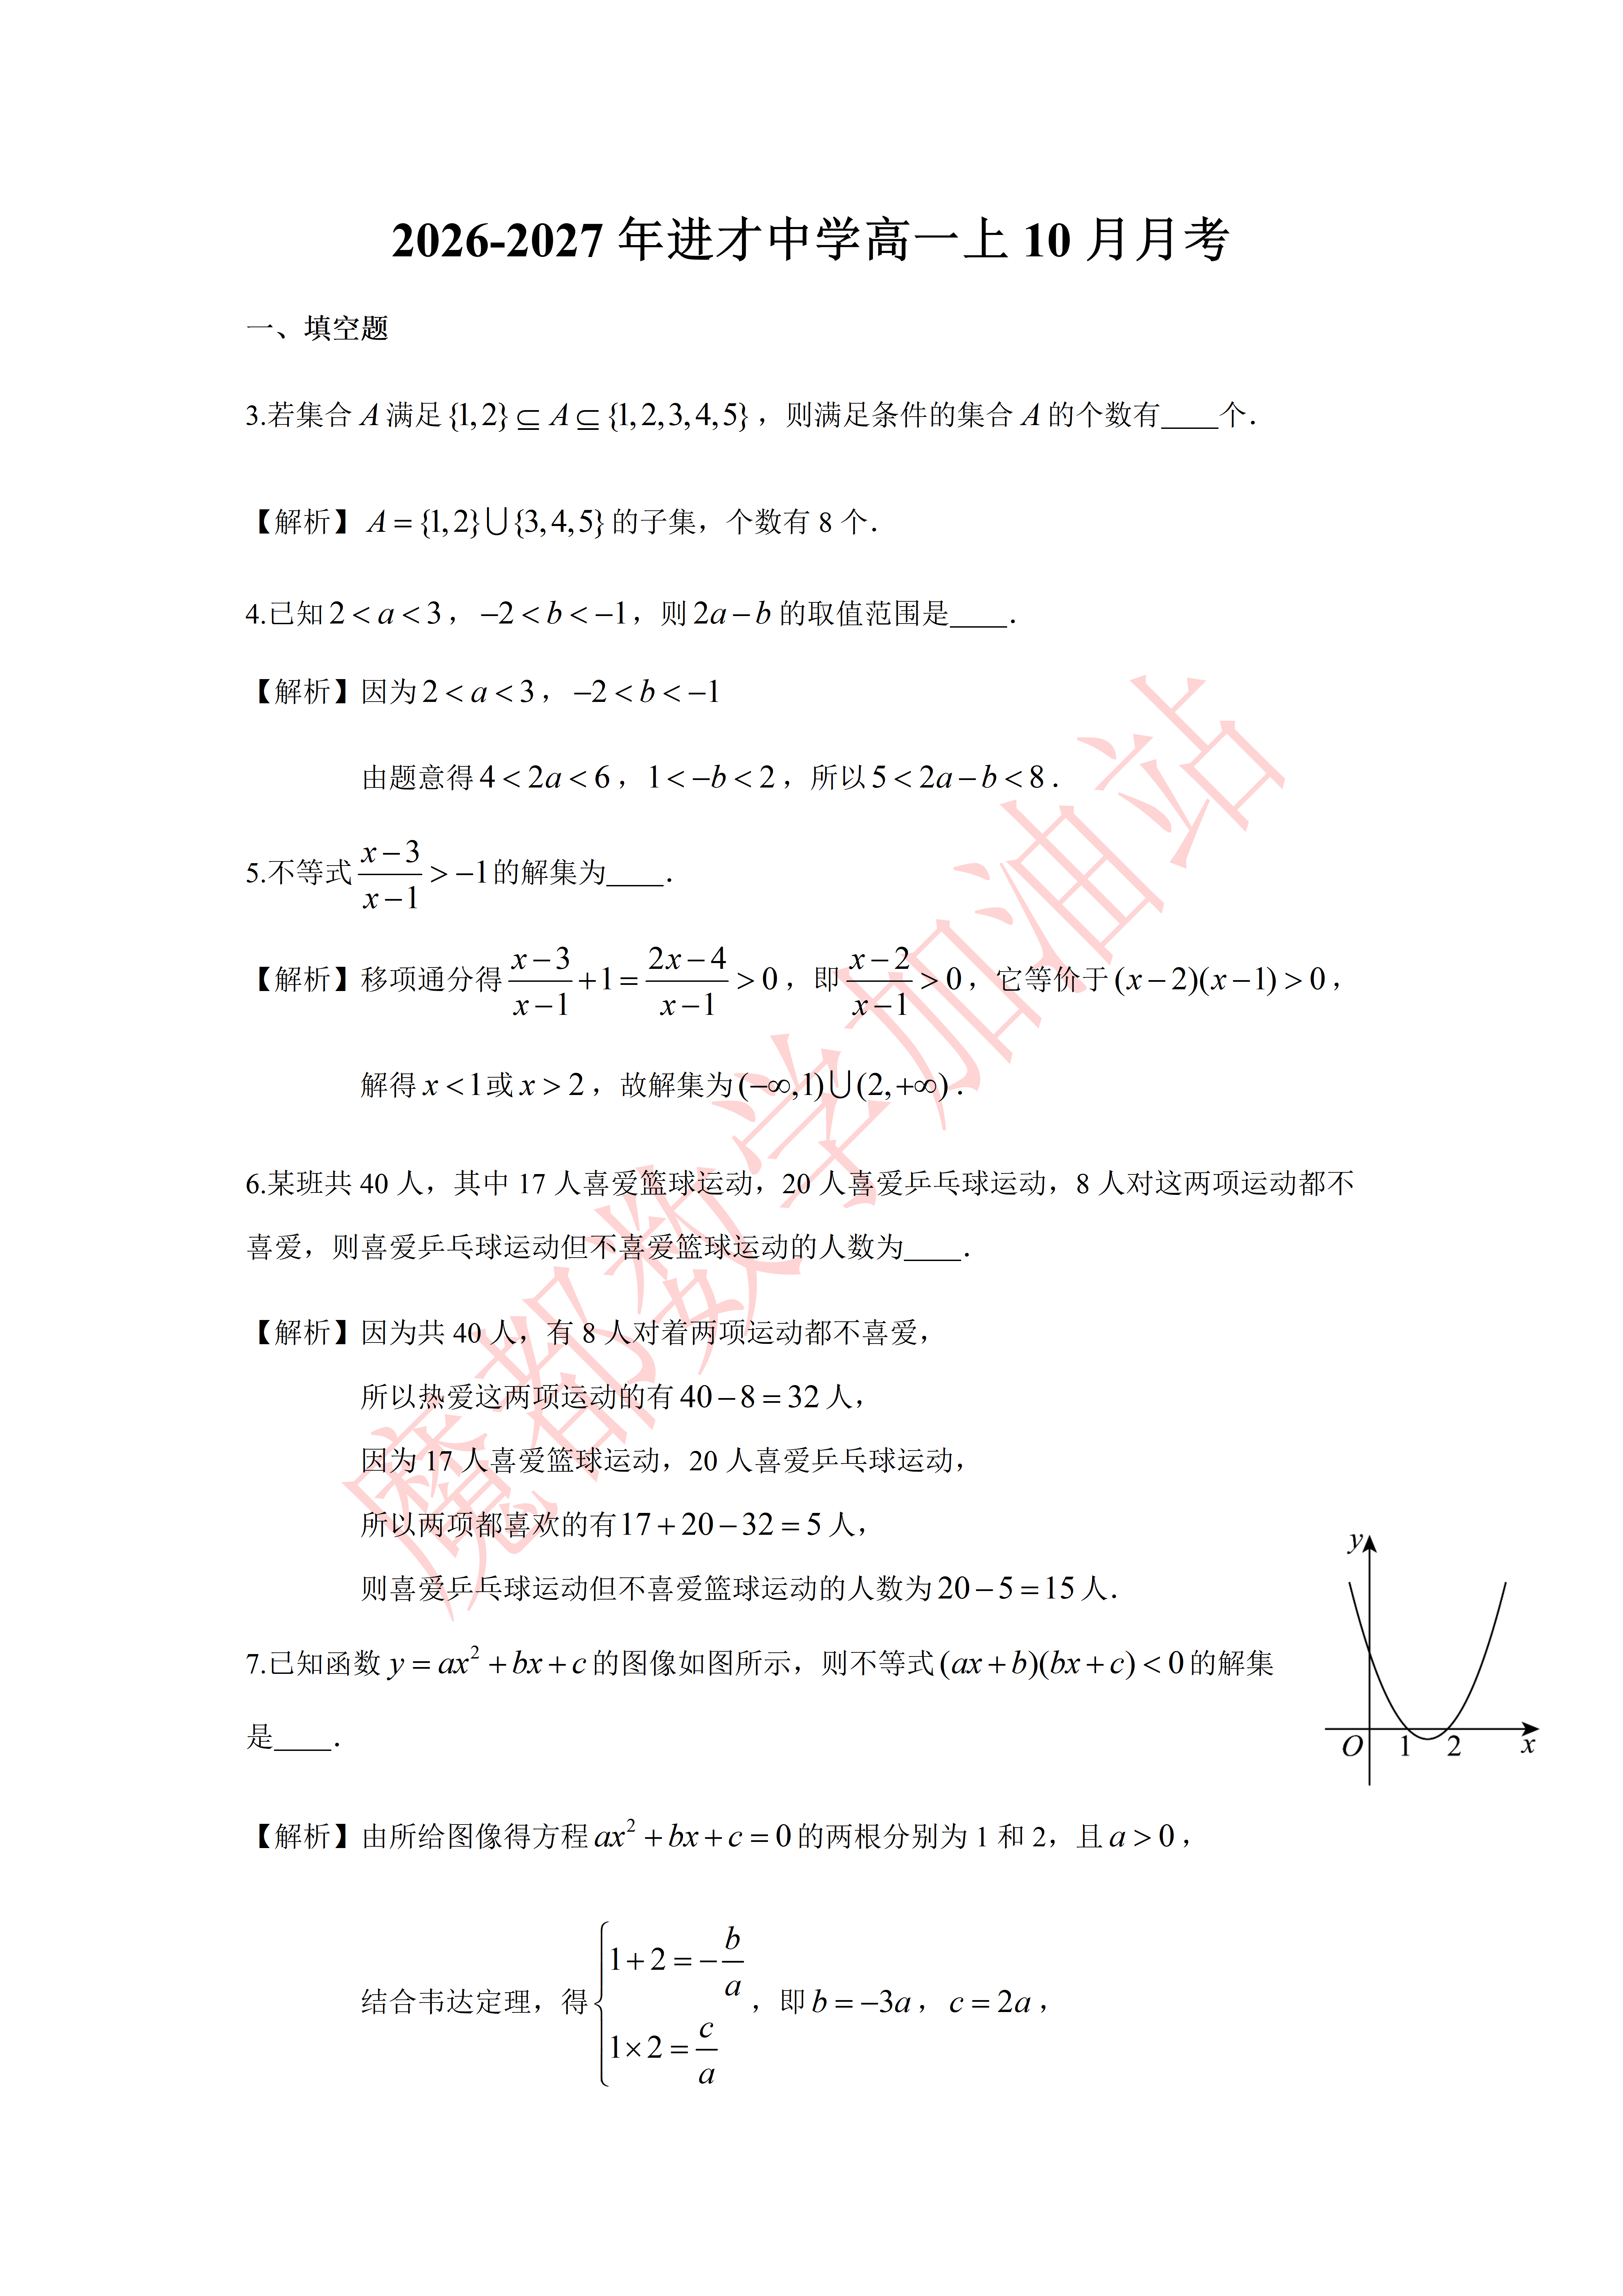
\includegraphics[width=.22\linewidth,trim=3879bp 1490bp 238bp 4492bp,clip]{../原图/高一60_进才中学_10月月考/01.png}
\end{center}

\ifanswer
\solbegin
\step{由所给图像得方程 $ax^2+bx+c=0$ 的两根分别为 1 和 2，且 $a>0$，}
\step{结合韦达定理，得 $\begin{cases}1+2=-\dfrac ba\\ 1\times2=\dfrac ca\end{cases}$，即 $b=-3a$，$c=2a$，}
\step{所以不等式 $(ax+b)(bx+c)<0$ 即 $(ax-3a)(-3ax+2a)<0$，}
\step{化简得 $(x-3)(3x-2)>0$，解得 $x<\dfrac23$ 或 $x>3$，}
\step{所以不等式 $(ax+b)(bx+c)<0$ 的解集是 $(-\infty,\dfrac23)\cup(3,+\infty)$.}
\solend
\fi

\item 已知集合 $A=\{x\mid ax=6\}$，满足 $A\subseteq\Z$，则整数 $a$ 的所有可能取值有\blankline[4.4em]个.

\ifanswer
\solbegin
\step{当 $a=0$ 时，$A=\varnothing$，而 $\varnothing\subseteq\Z$，满足题意，}
\step{当 $a\neq0$ 时，$A=\left\{\dfrac6a\right\}$，要使 $A\subseteq\Z$，则 $\dfrac6a\in\Z$，所以 $a=\pm1,\pm2,\pm3,\pm6$，}
\step{综上，整数 $a$ 的可能取值为 0，$\pm1$，$\pm2$，$\pm3$，$\pm6$，共 9 个.}
\solend
\fi

\item 设关于 $x$ 的方程 $x^2+kx+n=0$ 有两个不同实根 $x_1$、$x_2$，且 $\dfrac1{x_1}+\dfrac1{x_2}=2$，则实数 $n$ 的取值范围是\blankline[4.4em].

\ifanswer
\solbegin
\step{由于方程 $x^2+kx+n=0$ 有两个不同实根 $x_1$、$x_2$，}
\step{因此 $\Delta=k^2-4n>0$，$x_1+x_2=-k$，$x_1x_2=n$，}
\step{由 $\dfrac1{x_1}+\dfrac1{x_2}=\dfrac{x_1+x_2}{x_1x_2}=\dfrac{-k}{n}=2$，得 $k=-2n$，}
\step{因此 $\Delta=k^2-4n=4n^2-4n>0$，解得 $n<0$ 或 $n>1$，}
\step{则实数 $n$ 的取值范围是 $(-\infty,0)\cup(1,+\infty)$.}
\solend
\fi

\item 某船从甲地沿河顺流航行 $75\mathrm{km}$，到达乙码头，停留 $30\mathrm{min}$ 后再逆流航行 $126\mathrm{km}$ 到达丙地，若水流速度为 $4\mathrm{km/h}$，且该船要在 $5\mathrm{h}$ 内完成航行任务，那么船的速度至少达到\blankline[4.4em]$\mathrm{km/h}$.

\ifanswer
\solbegin
\step{设该轮船在静水中的速度是 $x$ 千米/小时，水流速度是 4 千米/小时，}
\step{由题意得 $\dfrac{75}{4+x}+0.5+\dfrac{126}{x-4}\leqslant5$，即 $9x^2-402x-552\geqslant0$，解得 $x\geqslant46$，}
\step{答：该船的速度至少是 46 千米/小时.}
\solend
\fi

\item 设实数 $a,b,c$ 满足 $a^2+b^2\leqslant c<1$，则 $a+\dfrac12b+c$ 的最小值为\blankline[4.4em].

\ifanswer
\solbegin
\step{因为 $c\geqslant a^2+b^2$，}
\step{所以 $a+\dfrac12b+c\geqslant a+\dfrac12b+a^2+b^2=\left(a+\dfrac12\right)^2+\left(b+\dfrac14\right)^2-\dfrac5{16}\geqslant-\dfrac5{16}$，}
\step{当 $a=-\dfrac12,b=-\dfrac14,c=a^2+b^2=\dfrac5{16}$（此时 $c<1$ 成立）时取到等号，}
\step{故最小值为 $-\dfrac5{16}$.}
\solend
\fi

\item 已知集合 $A=\{x\in\N^*\mid1\leqslant x\leqslant2026\}$. 设集合 $B=\{b_1,b_2,b_3,\cdots,b_n\}$ 满足 $B\subseteq A$，且对任意的 $b_i$、$b_j$、$b_k\in B(i$、$j$、$k\in\{1,2,3,\cdots,n\})$，存在 $m\in\N^*$，使得 $b_i+b_j+b_k=39m$，则 $n$ 的最大值为\blankline[4.4em].

\ifanswer
\solbegin
\step{因为 $39=1\times39=3\times13$，所以 $n$ 的最大值大于 3，}
\step{若对任意的 $b_i$、$b_j$、$b_k\in B$，存在 $m\in\N^*$，使得 $b_i+b_j+b_k=39m$，}
\step{则集合 $B$ 的元素除以 39 的余数均为 0 或均为 13 或均为 26，}
\step{即 $B=\{39,78,\cdots,39n\}$ 或 $B=\{13,52,\cdots,39n-26\}$}
\step{或 $B=\{26,65,\cdots,39n-13\}$，}
\step{若 $B=\{39,78,\cdots,39n\}$，则 $39n\leqslant2026$，}
\step{解得 $n\leqslant\dfrac{2026}{39}\in(51,52)$，此时 $n$ 的最大值为 51；}
\step{若 $B=\{13,52,\cdots,39n-26\}$，则 $39n-26\leqslant2026$，}
\step{解得 $n\leqslant\dfrac{684}{13}\in(52,53)$，此时 $n$ 的最大值为 52；}
\step{若 $B=\{26,65,\cdots,39n-13\}$，则 $39n-13\leqslant2026$，}
\step{解得 $n\leqslant\dfrac{2039}{39}\in(52,53)$，此时 $n$ 的最大值为 52；}
\step{综上，$n$ 的最大值为 52.}
\solend
\fi

\end{enumerate}

\bigsec{二、选择题}

\begin{enumerate}
\setcounter{enumi}{12}

% 第 13 题原卷无【答案】/【解析】段，答案“B”直接印在题干括号内，
% 按 高一53 第 13 题的成例括号留空、答案另提为 \ans{}（见文件头）
\item 已知 $a$、$b\in\R$，则“$|a|>|b|$”是“$a>|b|$”的\mbox{（\quad）}

\keepwithprev
A. 充分不必要条件\qquad B. 必要不充分条件

C. 充要条件\qquad D. 既不充分也不必要条件

\ifanswer
\ans{$B$}
\fi

\item 如果关于 $x$ 的一元二次方程 $x^2+2mx+(m+2)=0$ 有一正根一负根，那么 $m$ 的取值范围为\mbox{（\quad）}

\keepwithprev
A. $(-2,-1)$\qquad B. $(-1,2)$

C. $(-\infty,-1)\cup(2,+\infty)$\qquad D. $(-\infty,-2)$

\ifanswer
\solbegin
\step{设两根为 $x_1,x_2$，方程有一正根一负根，则 $\begin{cases}x_1x_2=m+2<0\\ \Delta=4m^2-4(m+2)>0\end{cases}$，}
\step{解得 $m<-2$，故选 $D$.}
\solend
\fi

\item 若不等式 $|3x-a|\leqslant x+2$ 的解集包含集合 $[0,1]$，则实数 $a$ 的取值范围为\mbox{（\quad）}

\keepwithprev
A. $[0,2]$\qquad B. $[0,1]$

C. $[1,2]$\qquad D. $(1,2)$

\ifanswer
\solbegin
% 原卷“法一：”“法二：”排红色加粗（全卷唯一红字），本稿按全稿子题标号样式排 \stepm
% （详见文件头“与原卷的排版差异”⑦）
\stepm{法一：}{不等式 $|3x-a|\leqslant x+2$ 化为 $2x-2\leqslant a\leqslant4x+2$，}
% 原卷此句缺动词（疑漏“对”字），照录未改（见文件头“原卷存疑”④）
\step{$[0,1]$ 使 $2x-2\leqslant a\leqslant4x+2$ 成立，则 $0\leqslant a\leqslant2$，故选 $A$.}
\stepm{法二：}{将两边平方整理得 $8x^2-(6a+4)x+a^2-4\leqslant0$ 对 $[0,1]$ 恒成立，}
\step{则有 $\begin{cases}a^2-4\leqslant0\\ a^2-6a\leqslant0\end{cases}$，解得 $0\leqslant a\leqslant2$，故选 $A$.}
\solend
\fi

\item 数学组 Y 老师在白纸上写下以下四个命题：

①这四个命题中至少有一个是真的；②这四个命题中至少有两个是真的；

③这四个命题中至少有两个是假的；④这四个命题中至少有一个是假的；

每个命题非真即假. 问 Y 老师在纸上写的假命题有几个？\mbox{（\quad）}

\keepwithprev
A. 0\qquad B. 1

C. 2\qquad D. 3

\ifanswer
\solbegin
\step{设四个命题中真命题的个数为 $t$，则①真 $\iff t\geqslant1$，②真 $\iff t\geqslant2$，}
\step{③真 $\iff t\leqslant2$，④真 $\iff t\leqslant3$.}
\step{逐一检验：$t=0$ 时③④为真，应为 $t=2$，矛盾；}
\step{$t=1$ 时①③④为真，应为 $t=3$，矛盾；}
\step{$t=2$ 时四个命题全为真，应为 $t=4$，矛盾；}
\step{$t=3$ 时①②④为真、③为假，恰有 3 个真命题，符合；}
\step{$t=4$ 时①②为真，应为 $t=2$，矛盾.}
\step{所以恰有 1 个假命题，故选 $B$.}
\solend
\fi

\end{enumerate}

\bigsec{三、解答题}

\begin{enumerate}
\setcounter{enumi}{16}

\item 已知：$x\in\R$，$a=x^2-1$，$b=4x+5$. 求证：$a$、$b$ 中至少有一个大于等于 0.

\ifanswer
\solbegin
\step{假设 $a$、$b$ 都小于 0，即 $a<0$，$b<0$，则 $a+b<0$.}
\step{又 $a+b=x^2-1+4x+5=x^2+4x+4=(x+2)^2\geqslant0$，}
\step{这与假设所得 $a+b<0$ 矛盾，故假设不成立，}
\step{所以 $a$、$b$ 中至少有一个大于等于 0.}
\solend
\fi

\ansspace[6]

% 原卷 A、B 两个集合定义之间排半角逗号“,”（5 倍放大核，右侧字距 19px，与全卷全角“，”的 65—79px 字距判然有别）；
% 本稿原误抄为全角“，”——已照录原卷半角（见文件头“与原卷的排版差异”⑤）
\item 已知集合 $A=\{x\mid4\leqslant x\leqslant12\}$,$B=\{x\mid a\leqslant x\leqslant2a+1\}$.

（1）若 $a=2$，求 $\overline A\cap B$；

（2）已知 $A\cup B=A$，求实数 $a$ 的取值范围.

\ifanswer
\solbegin
\stepm{(1)}{当 $a=2$ 时，$B=\{x\mid2\leqslant x\leqslant5\}$，}
\step{而 $A=\{x\mid4\leqslant x\leqslant12\}$，则 $\overline A=(-\infty,4)\cup(12,+\infty)$，所以 $\overline A\cap B=[2,4)$.}
\stepm{(2)}{$A\cup B=A$ 即 $B\subseteq A$.}
\stepm{①}{当 $B=\varnothing$ 时，$a>2a+1$，即 $a<-1$，符合；}
\stepm{②}{当 $B\neq\varnothing$ 时，需 $a\leqslant2a+1$ 且 $a\geqslant4$ 且 $2a+1\leqslant12$，即 $4\leqslant a\leqslant\dfrac{11}2$.}
\step{综上，$a$ 的取值范围是 $(-\infty,-1)\cup\left[4,\dfrac{11}2\right]$.}
\solend
\fi

\ansspace[8]

\item （1）若关于 $x$ 的不等式 $ax^2-3x+2<0$ 的解集不是空集，求实数 $a$ 的取值范围；

（2）求关于 $x$ 的不等式 $ax^2-3x+2>ax-1$ 的解集.

\ifanswer
\solbegin
\stepm{(1)}{若 $a>0$，关于 $x$ 的不等式 $ax^2-3x+2<0$ 的解集不空，}
\step{所以一元二次方程 $ax^2-3x+2=0$ 的判别式大于零，}
\step{即 $(-3)^2-8a>0\Rightarrow a<\dfrac98$，结合 $a>0$ 得 $0<a<\dfrac98$；}
\step{若 $a\leqslant0$，则关于 $x$ 的不等式 $ax^2-3x+2<0$ 的解集不是空集；}
\step{综上，实数 $a$ 的取值范围是 $\left(-\infty,\dfrac98\right)$.}
\stepm{(2)}{$ax^2-3x+2>ax-1\Rightarrow ax^2-(a+3)x+3>0\Rightarrow(ax-3)(x-1)>0$，}
\step{当 $a=0$ 时，不等式为 $x-1<0$，不等式的解集为 $\{x\mid x<1\}$；}
\step{当 $a<0$ 时，不等式化为 $\left(x-\dfrac3a\right)(x-1)<0$，}
\step{不等式的解集为 $\left\{x\mid\dfrac3a<x<1\right\}$，}
\step{当 $a>0$ 时，方程 $ax^2-3x+2=ax-1$ 的两个根分别为：$\dfrac3a,1$.}
\step{当 $a=3$ 时，两根相等，故不等式的解集为 $\{x\mid x\neq1\}$；}
\step{当 $a>3$ 时，$\dfrac3a<1$，不等式的解集为 $\left\{x\mid x<\dfrac3a\right.$ 或 $\left.x>1\right\}$；}
\step{当 $0<a<3$ 时，$\dfrac3a>1$，不等式的解集为 $\left\{x\mid x<1\right.$ 或 $\left.x>\dfrac3a\right\}$；}
\step{综上所述，当 $a<0$ 时，不等式的解集为 $\left\{x\mid\dfrac3a<x<1\right\}$，}
\step{当 $a=0$ 时，不等式的解集为 $\{x\mid x<1\}$，}
\step{当 $0<a<3$ 时，不等式的解集为 $\left\{x\mid x<1\right.$ 或 $\left.x>\dfrac3a\right\}$，}
\step{当 $a=3$ 时，不等式的解集为 $\{x\mid x\neq1\}$，}
\step{当 $a>3$ 时，不等式的解集为 $\left\{x\mid x<\dfrac3a\right.$ 或 $\left.x>1\right\}$.}
\solend
\fi

\ansspace[8]

\item 设命题 $p$：对任意 $x\in\R$，使得不等式 $mx^2-mx+2>0$ 恒成立；命题 $q$：存在 $0\leqslant x\leqslant3$，不等式 $2x-2\geqslant|m|$ 成立.

（1）若 $p$ 为真命题，求实数 $m$ 的取值范围；

（2）若 $p$、$q$ 有且只有一个是真命题，求实数 $m$ 的取值范围.

\ifanswer
\solbegin
\stepm{(1)}{因为 $p:\forall x\in\R$，$mx^2-mx+2>0$ 为真命题，}
\step{所以当 $m=0$ 时，不等式为 $2>0$，在 $\R$ 上恒成立，符合题意；}
\step{当 $m\neq0$ 时，$\begin{cases}m>0\\ \Delta=m^2-8m<0\end{cases}$，解得 $0<m<8$.}
\step{综上，实数 $m$ 的取值范围为 $[0,8)$.}
\stepm{(2)}{若 $q$ 为真命题，即 $q:\exists0\leqslant x\leqslant3$，$2x-2\geqslant|m|$，}
\step{则对于 $0\leqslant x\leqslant3$，$(2x-2)_{max}\geqslant|m|$.}
\step{由于 $0\leqslant x\leqslant3$，$2x-2\in[-2,4]$，所以 $|m|\leqslant4$，解得 $-4\leqslant m\leqslant4$，}
\step{又因为 $p$、$q$ 有且只有一个是真命题，}
\step{所以当 $p$ 真 $q$ 假时，$\begin{cases}0\leqslant m<8\\ m<-4\text{或}m>4\end{cases}$，解得 $4<m<8$；}
\step{当 $p$ 假 $q$ 真时，$\begin{cases}m<0\text{或}m\geqslant8\\ -4\leqslant m\leqslant4\end{cases}$，解得 $-4\leqslant m<0$；}
\step{综上，实数 $m$ 的取值范围为 $[-4,0)\cup(4,8)$.}
\solend
\fi

\ansspace[10]

\item 已知集合 $A=\{a_1,a_2,\cdots,a_k\}(k\geqslant2)$. 其中 $a_i\in\N^*(i=1,2,\cdots,k)$. 若对于任意的 $a\in A$，总有 $\dfrac1a\notin A$，则称集合 $A$ 具有性质 $P$. 由 $A$ 中的元素构成两个相应的集合：$S=\{(a,b)\mid a\in A,b\in A,ab\in A\}$，$T=\left\{(a,b)\mid a\in A,b\in A,\dfrac ab\in A\right\}$，其中 $(a,b)$ 是有序数对，集合 $S$ 和 $T$ 中的元素个数分别为 $m$ 和 $n$.

（1）检验集合 $\{2,3,6\}$ 与 $\{1,2,4\}$ 是否具有性质 $P$，并对其中具有性质 $P$ 的集合，写出相应的集合 $S$ 和 $T$；

（2）对任何具有性质 $P$ 的集合 $A$，$n$ 的最大值为多少？（直接写出答案，无需说明理由）；

% 原卷题干的小问编号跳号：印作 (1)(2)(4)，本稿照录 (4)、未改成 (3)（见文件头“原卷存疑”①）
（4）判断 $m$ 和 $n$ 的大小关系，并证明你的结论.

\ifanswer
\solbegin
\stepm{(1)}{因为 $\dfrac12\in\{1,2,4\}$，所以 $\{1,2,4\}$ 不具有性质 $P$；}
\step{因为 $\dfrac12\notin\{2,3,6\}$，$\dfrac13\notin\{2,3,6\}$，$\dfrac16\notin\{2,3,6\}$，所以 $\{2,3,6\}$ 具有性质 $P$.}
\step{$S=\{(2,3),(3,2)\}$，$T=\{(6,2),(6,3)\}$；}
\stepm{(2)}{因为对于任意的 $a\in A$，总有 $\dfrac1a\notin A$，所以 $1\notin A$，}
% 原卷此处印作“$\{(a_i,a_i)\}\in T$”，与上一句“$1\notin A$”及下文“最多为 $C_k^2$”的推理
% 均不自洽（应为“$\notin$”），已 8 倍放大确认无斜线；照录未改（见文件头“原卷存疑”③）
\step{从而 $\{(a_i,a_i)\}\in T(i=1,2,\cdots,k)$.}
\step{因为 $a\in A,b\in A,\dfrac ab\in A$，所以当 $i\neq j$ 时，}
\step{$(a_i,a_j)\in T$ 和 $(a_j,a_i)\in T(i,j=1,2,\cdots,k)$ 至多有一个成立，}
\step{所以集合 $T$ 中的元素个数最多为 $C_k^2=\dfrac{k(k-1)}2$，即 $n\leqslant\dfrac{k(k-1)}2$.}
% 原卷【解析】把第 (4) 问标作“(3)”（与题干跳号相应），本稿照录未改（见文件头“原卷存疑”①）
\stepm{(3)}{$m=n$，证明如下：}
\step{①设 $(a,b)\in T$，则 $a\in A,b\in A,\dfrac ab\in A$. 设 $c=\dfrac ab$，则 $a=bc$，}
\step{故 $b\in A$，$c\in A$，$bc\in A$，从而 $(b,c)\in S$，}
\step{即对 $\forall(a,b)\in T$，总 $\exists c$ 使 $(b,c)\in S$，从而 $n\leqslant m$.}
\step{②设 $(p,q)\in S$，则 $p\in A$，$q\in A$，$pq\in A$.}
\step{设 $r=pq$，则 $q=\dfrac rp$，故 $r\in A,p\in A,\dfrac rp\in A$，从而 $(r,p)\in T$，}
\step{即对 $\forall(p,q)\in S$，总 $\exists r$ 使 $(r,p)\in T$，从而 $m\leqslant n$.}
\step{由①②得 $m=n$.}
\solend
\fi

\ansspace*[10]

\end{enumerate}

\end{document}
"
%
% 原文链接：https://mp.weixin.qq.com/s/2ZLKB3IONEDhcUAfAAYE2A。
% 公众号“魔都数学加油站”作者破晓于 2026-10-14 22:15 发布。
% 原图 9 张（`原图/高一60_进才中学_10月月考/01..09.png`）：第 1—8 页 4762×6735，
% 第 9 页 2560×3620（同一篇内两档分辨率）。
%
% 卷首标题：照卷面印作“2026--2027 年进才中学高一上 10 月月考”（公众号标题中的“上海市”
% 卷面标题行没有，本稿照卷面），年份区间按全稿惯例排 en dash。原卷只有一行标题、无副标题。
%
% 篇幅与题号：原卷自第 3 题起编号（第 1、2 题不在本卷内）。填空题 3—12（10 题）、
% 选择题 13—16（4 题）、解答题 17—21（5 题），共 19 题。本稿沿用原节与原题号，
% 只改排为全稿统一的大节样式（原卷小节标题为“一、填空题”“二、选择题”“三、解答题”）。
%
% 讲评版：原卷每题下直接印【答案】或【解析】。**只印【解析】的 18 题**，本稿按全稿口径
% 收进答案版、不另提 \ans{}——第 14、15、16 题的结论写在解析末句（“故选 D／A／B”），
% 亦照录在解析内。**第 13 题原卷没有任何【答案】/【解析】段**，答案“B”直接印在题干括号内
% （“（ B ）”），本稿按 高一53 第 13 题的成例把括号留空、答案另提为 \ans{$B$}（见下）。
%
% 副标题：原卷未印副标题。本稿按“知识模块”口径标作“集合与常用逻辑用语、不等式”：
% 19 题中集合与常用逻辑用语 10 题（第 3、6、8、12、13、16、17、18、20、21 题，
% 含子集计数、韦恩图容斥、集合运算、命题与充要条件、反证法、新定义），
% 不等式 9 题（含不等式性质、分式不等式、二次函数与解集、韦达定理与判别式、
% 不等式应用、最值、根的分布、绝对值不等式恒成立、含参二次不等式：第 4、5、7、9、10、
% 11、14、15、19 题），两类均远超三分之一，故并标。口径同 高一46、高一47、高一48、
% 高一51—高一59。
%
% 与原卷的排版差异：
%   ① 原卷每题下直接印【答案】/【解析】，本稿按全稿惯例将答案与解析置于答案版，试卷版保持干净；
%   ② 原卷未印副标题，本稿按“知识模块”口径补出；
%   ③ 原卷填空横线约两个字宽，本稿按全稿惯例统一排 \blankline[4.4em]；
%   ④ 原卷实数集排斜体 $R$（第 13、17、20 题）、正整数集排 $N^*$（第 12、21 题）、
%      整数集排粗体 $\mathbf{Z}$（第 8 题），本稿按全稿惯例改用 $\R$、$\N^*$、$\Z$；
%      空集记号统一为 \varnothing；
%   ⑤ 原卷在数学式内多处用半角逗号（如 $x_1,x_2$、$a,b\in R$，以及第 18 题题干
%      $A=\{x\mid4\leqslant x\leqslant12\}$,$B=\{x\mid a\leqslant x\leqslant2a+1\}$ 之间的逗号），
%      均照录未强改（第 18 题题干那一处本稿首轮曾误作全角“，”，第二轮已订正）；
%      句末句点按全稿惯例排西文句点；
%   ⑥ 第 13 题印在题干括号内的答案“B”移入 \ans{}，见上；
%   ⑦ 第 15 题【解析】的“法一：”“法二：”标号原卷排**红色加粗**（全卷唯一的红字，2 处），
%      本稿按全稿子题标号样式排 \stepm{法一：}{…}、\stepm{法二：}{…}（加粗着色、不改黑色
%      基调），冒号照原卷排全角；
%   ⑧ 第 7 题的图像原卷排在题干右侧（与题干第 1 行同高），本稿居中排在题干之后；
%      图自原图第 01 页裁切（trim），不另存图片文件；
%   ⑨ 原卷第 10 题的长度与速度单位原卷排斜体（$75km$、$4km/h$ 等），本稿按全稿惯例
%      改排正体 $\mathrm{km}$、$\mathrm{km/h}$（同 高一56 第 13 题）；每道解答题原卷未留
%      作答空白，本稿按全稿惯例加 \ansspace。
%
% 原卷存疑（照录未改，见源码中该处上方注释）：
%   ① 第 21 题题干的小问编号**跳号**：印作 (1)(2)(4)，而紧随其后的【解析】按 (1)(2)(3) 写
%      —— 题干第 (4) 问实为第 (3) 问。本稿题干照录 (1)(2)(4)、解析照录 (3)，未改
%      （与 高一22 第 16 题“解析误标 (2)”同一处理）。
%   ② 第 6 题【解析】“有 8 人**对着**两项运动都不喜爱”，“对着”疑为“对这”之误，照录未改。
%   ③ 第 21(2) 题【解析】首行“所以 $1\notin A$，从而 $\{(a_i,a_i)\}\in T(i=1,2,\cdots,k)$”
%      —— 由 $1\notin A$ 应得 $(a_i,a_i)\notin T$（因 $a_i/a_i=1$），与紧随的“$T$ 中元素
%      个数最多为 $C_k^2$”这一推理亦只有“$\notin$”才自洽；原卷此处印作“$\in$”，
%      已 8 倍放大确认无斜线。**照录原卷的 $\in$、未改**。
%   ④ 第 15 题【解析】法一“$[0,1]$ 使 $2x-2\leqslant a\leqslant4x+2$ 成立”一句缺动词
%      （疑漏“对”字），照录未改。
%
\documentclass[a4paper,11pt]{article}
\usepackage{common}

\begin{document}

\examtitlest[3]{2026--2027 年进才中学高一上 10 月月考}{集合与常用逻辑用语、不等式}

\bigsec{一、填空题}

\begin{enumerate}
\setcounter{enumi}{2}

\item 若集合 $A$ 满足 $\{1,2\}\subseteq A\subseteq\{1,2,3,4,5\}$，则满足条件的集合 $A$ 的个数有\blankline[4.4em]个.

\ifanswer
\solbegin
\step{$A=\{1,2\}\cup\{3,4,5\}$ 的子集，个数有 8 个.}
\solend
\fi

\item 已知 $2<a<3$，$-2<b<-1$，则 $2a-b$ 的取值范围是\blankline[4.4em].

\ifanswer
\solbegin
\step{因为 $2<a<3$，$-2<b<-1$，}
\step{由题意得 $4<2a<6$，$1<-b<2$，所以 $5<2a-b<8$.}
\solend
\fi

\item 不等式 $\dfrac{x-3}{x-1}>-1$ 的解集为\blankline[4.4em].

\ifanswer
\solbegin
\step{移项通分得 $\dfrac{x-3}{x-1}+1=\dfrac{2x-4}{x-1}>0$，即 $\dfrac{x-2}{x-1}>0$，它等价于 $(x-2)(x-1)>0$，}
\step{解得 $x<1$ 或 $x>2$，故解集为 $(-\infty,1)\cup(2,+\infty)$.}
\solend
\fi

\item 某班共 40 人，其中 17 人喜爱篮球运动，20 人喜爱乒乓球运动，8 人对这两项运动都不喜爱，则喜爱乒乓球运动但不喜爱篮球运动的人数为\blankline[4.4em].

\ifanswer
\solbegin
% 原卷作“对着两项运动都不喜爱”（疑为“对这”之误），照录未改（见文件头“原卷存疑”②）
\step{因为共 40 人，有 8 人对着两项运动都不喜爱，}
\step{所以热爱这两项运动的有 $40-8=32$ 人，}
\step{因为 17 人喜爱篮球运动，20 人喜爱乒乓球运动，}
\step{所以两项都喜欢的有 $17+20-32=5$ 人，}
\step{则喜爱乒乓球运动但不喜爱篮球运动的人数为 $20-5=15$ 人.}
\solend
\fi

\item 已知函数 $y=ax^2+bx+c$ 的图像如图所示，则不等式 $(ax+b)(bx+c)<0$ 的解集是\blankline[4.4em].

% 原图第 01 页题干右侧的图像直接裁取。裁框取图外框 x 3887–4516、y 4500–5237
% （四周各留约 8px），trim=左 3879bp／下 1490bp／右 238bp／上 4492bp
% （页宽 4762、页高 6735）。
\begin{center}
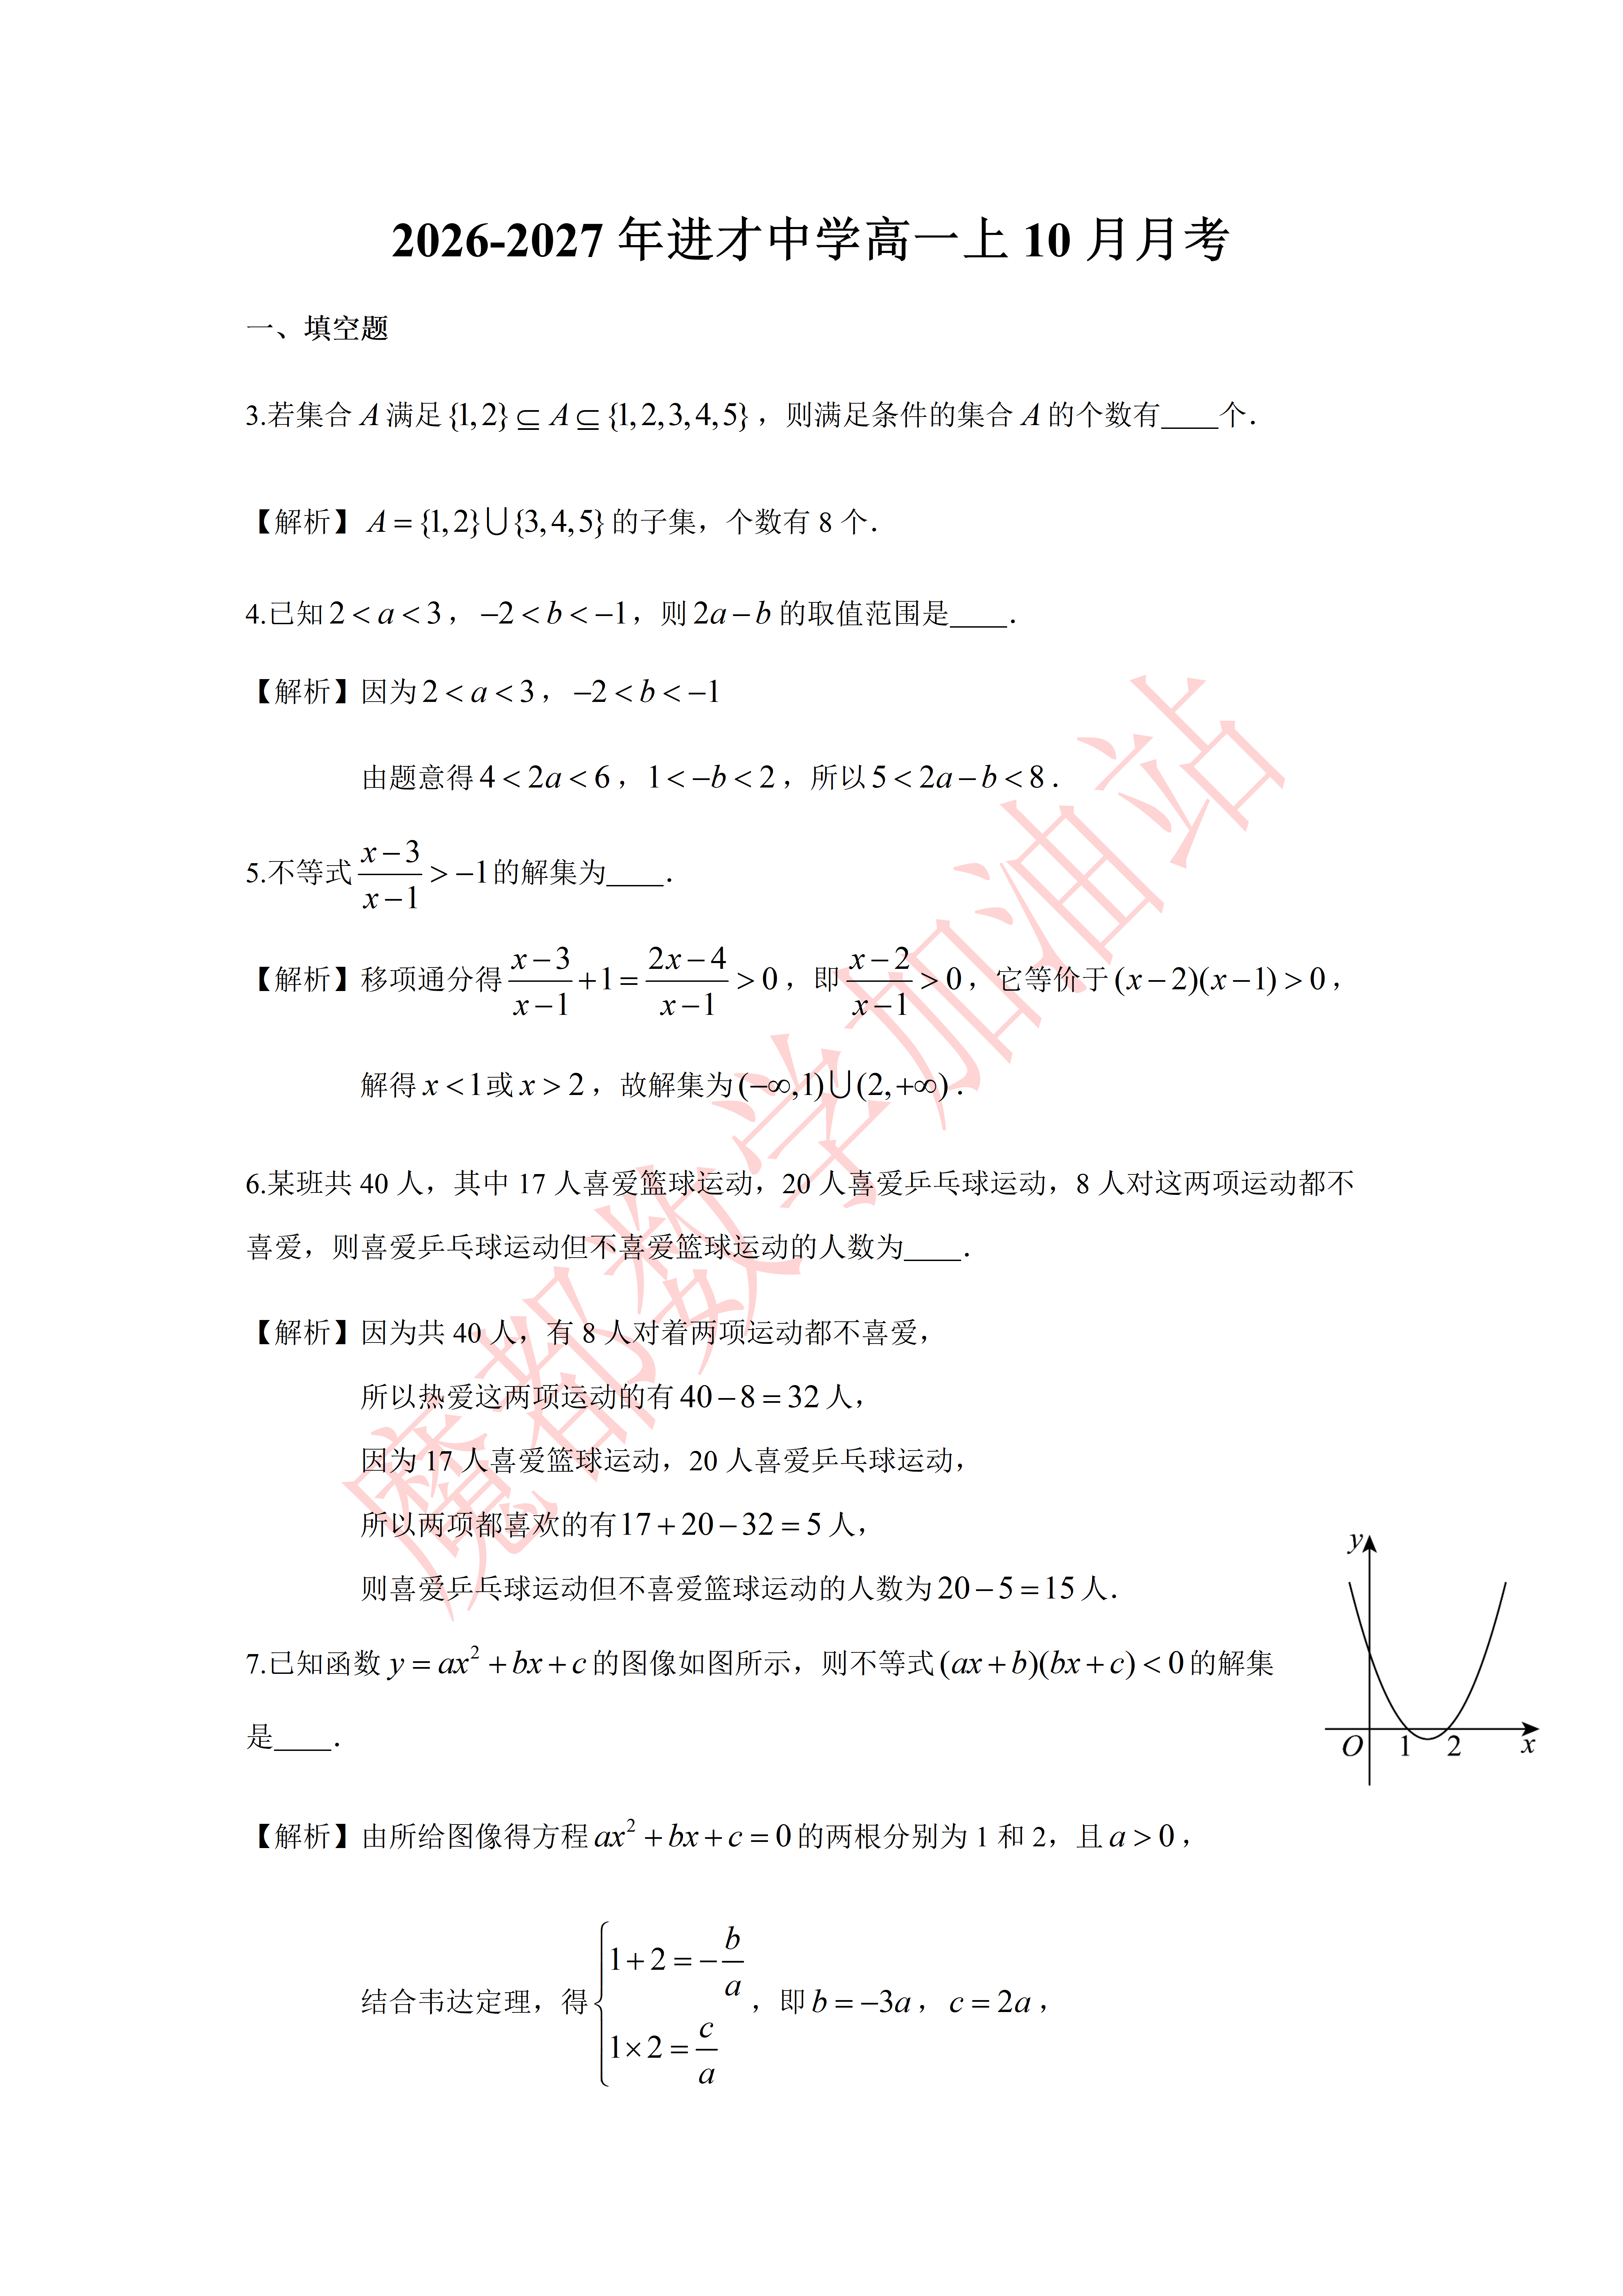
\includegraphics[width=.22\linewidth,trim=3879bp 1490bp 238bp 4492bp,clip]{../原图/高一60_进才中学_10月月考/01.png}
\end{center}

\ifanswer
\solbegin
\step{由所给图像得方程 $ax^2+bx+c=0$ 的两根分别为 1 和 2，且 $a>0$，}
\step{结合韦达定理，得 $\begin{cases}1+2=-\dfrac ba\\ 1\times2=\dfrac ca\end{cases}$，即 $b=-3a$，$c=2a$，}
\step{所以不等式 $(ax+b)(bx+c)<0$ 即 $(ax-3a)(-3ax+2a)<0$，}
\step{化简得 $(x-3)(3x-2)>0$，解得 $x<\dfrac23$ 或 $x>3$，}
\step{所以不等式 $(ax+b)(bx+c)<0$ 的解集是 $(-\infty,\dfrac23)\cup(3,+\infty)$.}
\solend
\fi

\item 已知集合 $A=\{x\mid ax=6\}$，满足 $A\subseteq\Z$，则整数 $a$ 的所有可能取值有\blankline[4.4em]个.

\ifanswer
\solbegin
\step{当 $a=0$ 时，$A=\varnothing$，而 $\varnothing\subseteq\Z$，满足题意，}
\step{当 $a\neq0$ 时，$A=\left\{\dfrac6a\right\}$，要使 $A\subseteq\Z$，则 $\dfrac6a\in\Z$，所以 $a=\pm1,\pm2,\pm3,\pm6$，}
\step{综上，整数 $a$ 的可能取值为 0，$\pm1$，$\pm2$，$\pm3$，$\pm6$，共 9 个.}
\solend
\fi

\item 设关于 $x$ 的方程 $x^2+kx+n=0$ 有两个不同实根 $x_1$、$x_2$，且 $\dfrac1{x_1}+\dfrac1{x_2}=2$，则实数 $n$ 的取值范围是\blankline[4.4em].

\ifanswer
\solbegin
\step{由于方程 $x^2+kx+n=0$ 有两个不同实根 $x_1$、$x_2$，}
\step{因此 $\Delta=k^2-4n>0$，$x_1+x_2=-k$，$x_1x_2=n$，}
\step{由 $\dfrac1{x_1}+\dfrac1{x_2}=\dfrac{x_1+x_2}{x_1x_2}=\dfrac{-k}{n}=2$，得 $k=-2n$，}
\step{因此 $\Delta=k^2-4n=4n^2-4n>0$，解得 $n<0$ 或 $n>1$，}
\step{则实数 $n$ 的取值范围是 $(-\infty,0)\cup(1,+\infty)$.}
\solend
\fi

\item 某船从甲地沿河顺流航行 $75\mathrm{km}$，到达乙码头，停留 $30\mathrm{min}$ 后再逆流航行 $126\mathrm{km}$ 到达丙地，若水流速度为 $4\mathrm{km/h}$，且该船要在 $5\mathrm{h}$ 内完成航行任务，那么船的速度至少达到\blankline[4.4em]$\mathrm{km/h}$.

\ifanswer
\solbegin
\step{设该轮船在静水中的速度是 $x$ 千米/小时，水流速度是 4 千米/小时，}
\step{由题意得 $\dfrac{75}{4+x}+0.5+\dfrac{126}{x-4}\leqslant5$，即 $9x^2-402x-552\geqslant0$，解得 $x\geqslant46$，}
\step{答：该船的速度至少是 46 千米/小时.}
\solend
\fi

\item 设实数 $a,b,c$ 满足 $a^2+b^2\leqslant c<1$，则 $a+\dfrac12b+c$ 的最小值为\blankline[4.4em].

\ifanswer
\solbegin
\step{因为 $c\geqslant a^2+b^2$，}
\step{所以 $a+\dfrac12b+c\geqslant a+\dfrac12b+a^2+b^2=\left(a+\dfrac12\right)^2+\left(b+\dfrac14\right)^2-\dfrac5{16}\geqslant-\dfrac5{16}$，}
\step{当 $a=-\dfrac12,b=-\dfrac14,c=a^2+b^2=\dfrac5{16}$（此时 $c<1$ 成立）时取到等号，}
\step{故最小值为 $-\dfrac5{16}$.}
\solend
\fi

\item 已知集合 $A=\{x\in\N^*\mid1\leqslant x\leqslant2026\}$. 设集合 $B=\{b_1,b_2,b_3,\cdots,b_n\}$ 满足 $B\subseteq A$，且对任意的 $b_i$、$b_j$、$b_k\in B(i$、$j$、$k\in\{1,2,3,\cdots,n\})$，存在 $m\in\N^*$，使得 $b_i+b_j+b_k=39m$，则 $n$ 的最大值为\blankline[4.4em].

\ifanswer
\solbegin
\step{因为 $39=1\times39=3\times13$，所以 $n$ 的最大值大于 3，}
\step{若对任意的 $b_i$、$b_j$、$b_k\in B$，存在 $m\in\N^*$，使得 $b_i+b_j+b_k=39m$，}
\step{则集合 $B$ 的元素除以 39 的余数均为 0 或均为 13 或均为 26，}
\step{即 $B=\{39,78,\cdots,39n\}$ 或 $B=\{13,52,\cdots,39n-26\}$}
\step{或 $B=\{26,65,\cdots,39n-13\}$，}
\step{若 $B=\{39,78,\cdots,39n\}$，则 $39n\leqslant2026$，}
\step{解得 $n\leqslant\dfrac{2026}{39}\in(51,52)$，此时 $n$ 的最大值为 51；}
\step{若 $B=\{13,52,\cdots,39n-26\}$，则 $39n-26\leqslant2026$，}
\step{解得 $n\leqslant\dfrac{684}{13}\in(52,53)$，此时 $n$ 的最大值为 52；}
\step{若 $B=\{26,65,\cdots,39n-13\}$，则 $39n-13\leqslant2026$，}
\step{解得 $n\leqslant\dfrac{2039}{39}\in(52,53)$，此时 $n$ 的最大值为 52；}
\step{综上，$n$ 的最大值为 52.}
\solend
\fi

\end{enumerate}

\bigsec{二、选择题}

\begin{enumerate}
\setcounter{enumi}{12}

% 第 13 题原卷无【答案】/【解析】段，答案“B”直接印在题干括号内，
% 按 高一53 第 13 题的成例括号留空、答案另提为 \ans{}（见文件头）
\item 已知 $a$、$b\in\R$，则“$|a|>|b|$”是“$a>|b|$”的\mbox{（\quad）}

\keepwithprev
A. 充分不必要条件\qquad B. 必要不充分条件

C. 充要条件\qquad D. 既不充分也不必要条件

\ifanswer
\ans{$B$}
\fi

\item 如果关于 $x$ 的一元二次方程 $x^2+2mx+(m+2)=0$ 有一正根一负根，那么 $m$ 的取值范围为\mbox{（\quad）}

\keepwithprev
A. $(-2,-1)$\qquad B. $(-1,2)$

C. $(-\infty,-1)\cup(2,+\infty)$\qquad D. $(-\infty,-2)$

\ifanswer
\solbegin
\step{设两根为 $x_1,x_2$，方程有一正根一负根，则 $\begin{cases}x_1x_2=m+2<0\\ \Delta=4m^2-4(m+2)>0\end{cases}$，}
\step{解得 $m<-2$，故选 $D$.}
\solend
\fi

\item 若不等式 $|3x-a|\leqslant x+2$ 的解集包含集合 $[0,1]$，则实数 $a$ 的取值范围为\mbox{（\quad）}

\keepwithprev
A. $[0,2]$\qquad B. $[0,1]$

C. $[1,2]$\qquad D. $(1,2)$

\ifanswer
\solbegin
% 原卷“法一：”“法二：”排红色加粗（全卷唯一红字），本稿按全稿子题标号样式排 \stepm
% （详见文件头“与原卷的排版差异”⑦）
\stepm{法一：}{不等式 $|3x-a|\leqslant x+2$ 化为 $2x-2\leqslant a\leqslant4x+2$，}
% 原卷此句缺动词（疑漏“对”字），照录未改（见文件头“原卷存疑”④）
\step{$[0,1]$ 使 $2x-2\leqslant a\leqslant4x+2$ 成立，则 $0\leqslant a\leqslant2$，故选 $A$.}
\stepm{法二：}{将两边平方整理得 $8x^2-(6a+4)x+a^2-4\leqslant0$ 对 $[0,1]$ 恒成立，}
\step{则有 $\begin{cases}a^2-4\leqslant0\\ a^2-6a\leqslant0\end{cases}$，解得 $0\leqslant a\leqslant2$，故选 $A$.}
\solend
\fi

\item 数学组 Y 老师在白纸上写下以下四个命题：

①这四个命题中至少有一个是真的；②这四个命题中至少有两个是真的；

③这四个命题中至少有两个是假的；④这四个命题中至少有一个是假的；

每个命题非真即假. 问 Y 老师在纸上写的假命题有几个？\mbox{（\quad）}

\keepwithprev
A. 0\qquad B. 1

C. 2\qquad D. 3

\ifanswer
\solbegin
\step{设四个命题中真命题的个数为 $t$，则①真 $\iff t\geqslant1$，②真 $\iff t\geqslant2$，}
\step{③真 $\iff t\leqslant2$，④真 $\iff t\leqslant3$.}
\step{逐一检验：$t=0$ 时③④为真，应为 $t=2$，矛盾；}
\step{$t=1$ 时①③④为真，应为 $t=3$，矛盾；}
\step{$t=2$ 时四个命题全为真，应为 $t=4$，矛盾；}
\step{$t=3$ 时①②④为真、③为假，恰有 3 个真命题，符合；}
\step{$t=4$ 时①②为真，应为 $t=2$，矛盾.}
\step{所以恰有 1 个假命题，故选 $B$.}
\solend
\fi

\end{enumerate}

\bigsec{三、解答题}

\begin{enumerate}
\setcounter{enumi}{16}

\item 已知：$x\in\R$，$a=x^2-1$，$b=4x+5$. 求证：$a$、$b$ 中至少有一个大于等于 0.

\ifanswer
\solbegin
\step{假设 $a$、$b$ 都小于 0，即 $a<0$，$b<0$，则 $a+b<0$.}
\step{又 $a+b=x^2-1+4x+5=x^2+4x+4=(x+2)^2\geqslant0$，}
\step{这与假设所得 $a+b<0$ 矛盾，故假设不成立，}
\step{所以 $a$、$b$ 中至少有一个大于等于 0.}
\solend
\fi

\ansspace[6]

% 原卷 A、B 两个集合定义之间排半角逗号“,”（5 倍放大核，右侧字距 19px，与全卷全角“，”的 65—79px 字距判然有别）；
% 本稿原误抄为全角“，”——已照录原卷半角（见文件头“与原卷的排版差异”⑤）
\item 已知集合 $A=\{x\mid4\leqslant x\leqslant12\}$,$B=\{x\mid a\leqslant x\leqslant2a+1\}$.

（1）若 $a=2$，求 $\overline A\cap B$；

（2）已知 $A\cup B=A$，求实数 $a$ 的取值范围.

\ifanswer
\solbegin
\stepm{(1)}{当 $a=2$ 时，$B=\{x\mid2\leqslant x\leqslant5\}$，}
\step{而 $A=\{x\mid4\leqslant x\leqslant12\}$，则 $\overline A=(-\infty,4)\cup(12,+\infty)$，所以 $\overline A\cap B=[2,4)$.}
\stepm{(2)}{$A\cup B=A$ 即 $B\subseteq A$.}
\stepm{①}{当 $B=\varnothing$ 时，$a>2a+1$，即 $a<-1$，符合；}
\stepm{②}{当 $B\neq\varnothing$ 时，需 $a\leqslant2a+1$ 且 $a\geqslant4$ 且 $2a+1\leqslant12$，即 $4\leqslant a\leqslant\dfrac{11}2$.}
\step{综上，$a$ 的取值范围是 $(-\infty,-1)\cup\left[4,\dfrac{11}2\right]$.}
\solend
\fi

\ansspace[8]

\item （1）若关于 $x$ 的不等式 $ax^2-3x+2<0$ 的解集不是空集，求实数 $a$ 的取值范围；

（2）求关于 $x$ 的不等式 $ax^2-3x+2>ax-1$ 的解集.

\ifanswer
\solbegin
\stepm{(1)}{若 $a>0$，关于 $x$ 的不等式 $ax^2-3x+2<0$ 的解集不空，}
\step{所以一元二次方程 $ax^2-3x+2=0$ 的判别式大于零，}
\step{即 $(-3)^2-8a>0\Rightarrow a<\dfrac98$，结合 $a>0$ 得 $0<a<\dfrac98$；}
\step{若 $a\leqslant0$，则关于 $x$ 的不等式 $ax^2-3x+2<0$ 的解集不是空集；}
\step{综上，实数 $a$ 的取值范围是 $\left(-\infty,\dfrac98\right)$.}
\stepm{(2)}{$ax^2-3x+2>ax-1\Rightarrow ax^2-(a+3)x+3>0\Rightarrow(ax-3)(x-1)>0$，}
\step{当 $a=0$ 时，不等式为 $x-1<0$，不等式的解集为 $\{x\mid x<1\}$；}
\step{当 $a<0$ 时，不等式化为 $\left(x-\dfrac3a\right)(x-1)<0$，}
\step{不等式的解集为 $\left\{x\mid\dfrac3a<x<1\right\}$，}
\step{当 $a>0$ 时，方程 $ax^2-3x+2=ax-1$ 的两个根分别为：$\dfrac3a,1$.}
\step{当 $a=3$ 时，两根相等，故不等式的解集为 $\{x\mid x\neq1\}$；}
\step{当 $a>3$ 时，$\dfrac3a<1$，不等式的解集为 $\left\{x\mid x<\dfrac3a\right.$ 或 $\left.x>1\right\}$；}
\step{当 $0<a<3$ 时，$\dfrac3a>1$，不等式的解集为 $\left\{x\mid x<1\right.$ 或 $\left.x>\dfrac3a\right\}$；}
\step{综上所述，当 $a<0$ 时，不等式的解集为 $\left\{x\mid\dfrac3a<x<1\right\}$，}
\step{当 $a=0$ 时，不等式的解集为 $\{x\mid x<1\}$，}
\step{当 $0<a<3$ 时，不等式的解集为 $\left\{x\mid x<1\right.$ 或 $\left.x>\dfrac3a\right\}$，}
\step{当 $a=3$ 时，不等式的解集为 $\{x\mid x\neq1\}$，}
\step{当 $a>3$ 时，不等式的解集为 $\left\{x\mid x<\dfrac3a\right.$ 或 $\left.x>1\right\}$.}
\solend
\fi

\ansspace[8]

\item 设命题 $p$：对任意 $x\in\R$，使得不等式 $mx^2-mx+2>0$ 恒成立；命题 $q$：存在 $0\leqslant x\leqslant3$，不等式 $2x-2\geqslant|m|$ 成立.

（1）若 $p$ 为真命题，求实数 $m$ 的取值范围；

（2）若 $p$、$q$ 有且只有一个是真命题，求实数 $m$ 的取值范围.

\ifanswer
\solbegin
\stepm{(1)}{因为 $p:\forall x\in\R$，$mx^2-mx+2>0$ 为真命题，}
\step{所以当 $m=0$ 时，不等式为 $2>0$，在 $\R$ 上恒成立，符合题意；}
\step{当 $m\neq0$ 时，$\begin{cases}m>0\\ \Delta=m^2-8m<0\end{cases}$，解得 $0<m<8$.}
\step{综上，实数 $m$ 的取值范围为 $[0,8)$.}
\stepm{(2)}{若 $q$ 为真命题，即 $q:\exists0\leqslant x\leqslant3$，$2x-2\geqslant|m|$，}
\step{则对于 $0\leqslant x\leqslant3$，$(2x-2)_{max}\geqslant|m|$.}
\step{由于 $0\leqslant x\leqslant3$，$2x-2\in[-2,4]$，所以 $|m|\leqslant4$，解得 $-4\leqslant m\leqslant4$，}
\step{又因为 $p$、$q$ 有且只有一个是真命题，}
\step{所以当 $p$ 真 $q$ 假时，$\begin{cases}0\leqslant m<8\\ m<-4\text{或}m>4\end{cases}$，解得 $4<m<8$；}
\step{当 $p$ 假 $q$ 真时，$\begin{cases}m<0\text{或}m\geqslant8\\ -4\leqslant m\leqslant4\end{cases}$，解得 $-4\leqslant m<0$；}
\step{综上，实数 $m$ 的取值范围为 $[-4,0)\cup(4,8)$.}
\solend
\fi

\ansspace[10]

\item 已知集合 $A=\{a_1,a_2,\cdots,a_k\}(k\geqslant2)$. 其中 $a_i\in\N^*(i=1,2,\cdots,k)$. 若对于任意的 $a\in A$，总有 $\dfrac1a\notin A$，则称集合 $A$ 具有性质 $P$. 由 $A$ 中的元素构成两个相应的集合：$S=\{(a,b)\mid a\in A,b\in A,ab\in A\}$，$T=\left\{(a,b)\mid a\in A,b\in A,\dfrac ab\in A\right\}$，其中 $(a,b)$ 是有序数对，集合 $S$ 和 $T$ 中的元素个数分别为 $m$ 和 $n$.

（1）检验集合 $\{2,3,6\}$ 与 $\{1,2,4\}$ 是否具有性质 $P$，并对其中具有性质 $P$ 的集合，写出相应的集合 $S$ 和 $T$；

（2）对任何具有性质 $P$ 的集合 $A$，$n$ 的最大值为多少？（直接写出答案，无需说明理由）；

% 原卷题干的小问编号跳号：印作 (1)(2)(4)，本稿照录 (4)、未改成 (3)（见文件头“原卷存疑”①）
（4）判断 $m$ 和 $n$ 的大小关系，并证明你的结论.

\ifanswer
\solbegin
\stepm{(1)}{因为 $\dfrac12\in\{1,2,4\}$，所以 $\{1,2,4\}$ 不具有性质 $P$；}
\step{因为 $\dfrac12\notin\{2,3,6\}$，$\dfrac13\notin\{2,3,6\}$，$\dfrac16\notin\{2,3,6\}$，所以 $\{2,3,6\}$ 具有性质 $P$.}
\step{$S=\{(2,3),(3,2)\}$，$T=\{(6,2),(6,3)\}$；}
\stepm{(2)}{因为对于任意的 $a\in A$，总有 $\dfrac1a\notin A$，所以 $1\notin A$，}
% 原卷此处印作“$\{(a_i,a_i)\}\in T$”，与上一句“$1\notin A$”及下文“最多为 $C_k^2$”的推理
% 均不自洽（应为“$\notin$”），已 8 倍放大确认无斜线；照录未改（见文件头“原卷存疑”③）
\step{从而 $\{(a_i,a_i)\}\in T(i=1,2,\cdots,k)$.}
\step{因为 $a\in A,b\in A,\dfrac ab\in A$，所以当 $i\neq j$ 时，}
\step{$(a_i,a_j)\in T$ 和 $(a_j,a_i)\in T(i,j=1,2,\cdots,k)$ 至多有一个成立，}
\step{所以集合 $T$ 中的元素个数最多为 $C_k^2=\dfrac{k(k-1)}2$，即 $n\leqslant\dfrac{k(k-1)}2$.}
% 原卷【解析】把第 (4) 问标作“(3)”（与题干跳号相应），本稿照录未改（见文件头“原卷存疑”①）
\stepm{(3)}{$m=n$，证明如下：}
\step{①设 $(a,b)\in T$，则 $a\in A,b\in A,\dfrac ab\in A$. 设 $c=\dfrac ab$，则 $a=bc$，}
\step{故 $b\in A$，$c\in A$，$bc\in A$，从而 $(b,c)\in S$，}
\step{即对 $\forall(a,b)\in T$，总 $\exists c$ 使 $(b,c)\in S$，从而 $n\leqslant m$.}
\step{②设 $(p,q)\in S$，则 $p\in A$，$q\in A$，$pq\in A$.}
\step{设 $r=pq$，则 $q=\dfrac rp$，故 $r\in A,p\in A,\dfrac rp\in A$，从而 $(r,p)\in T$，}
\step{即对 $\forall(p,q)\in S$，总 $\exists r$ 使 $(r,p)\in T$，从而 $m\leqslant n$.}
\step{由①②得 $m=n$.}
\solend
\fi

\ansspace*[10]

\end{enumerate}

\end{document}
"
%
% 原文链接：https://mp.weixin.qq.com/s/2ZLKB3IONEDhcUAfAAYE2A。
% 公众号“魔都数学加油站”作者破晓于 2026-10-14 22:15 发布。
% 原图 9 张（`原图/高一60_进才中学_10月月考/01..09.png`）：第 1—8 页 4762×6735，
% 第 9 页 2560×3620（同一篇内两档分辨率）。
%
% 卷首标题：照卷面印作“2026--2027 年进才中学高一上 10 月月考”（公众号标题中的“上海市”
% 卷面标题行没有，本稿照卷面），年份区间按全稿惯例排 en dash。原卷只有一行标题、无副标题。
%
% 篇幅与题号：原卷自第 3 题起编号（第 1、2 题不在本卷内）。填空题 3—12（10 题）、
% 选择题 13—16（4 题）、解答题 17—21（5 题），共 19 题。本稿沿用原节与原题号，
% 只改排为全稿统一的大节样式（原卷小节标题为“一、填空题”“二、选择题”“三、解答题”）。
%
% 讲评版：原卷每题下直接印【答案】或【解析】。**只印【解析】的 18 题**，本稿按全稿口径
% 收进答案版、不另提 \ans{}——第 14、15、16 题的结论写在解析末句（“故选 D／A／B”），
% 亦照录在解析内。**第 13 题原卷没有任何【答案】/【解析】段**，答案“B”直接印在题干括号内
% （“（ B ）”），本稿按 高一53 第 13 题的成例把括号留空、答案另提为 \ans{$B$}（见下）。
%
% 副标题：原卷未印副标题。本稿按“知识模块”口径标作“集合与常用逻辑用语、不等式”：
% 19 题中集合与常用逻辑用语 10 题（第 3、6、8、12、13、16、17、18、20、21 题，
% 含子集计数、韦恩图容斥、集合运算、命题与充要条件、反证法、新定义），
% 不等式 9 题（含不等式性质、分式不等式、二次函数与解集、韦达定理与判别式、
% 不等式应用、最值、根的分布、绝对值不等式恒成立、含参二次不等式：第 4、5、7、9、10、
% 11、14、15、19 题），两类均远超三分之一，故并标。口径同 高一46、高一47、高一48、
% 高一51—高一59。
%
% 与原卷的排版差异：
%   ① 原卷每题下直接印【答案】/【解析】，本稿按全稿惯例将答案与解析置于答案版，试卷版保持干净；
%   ② 原卷未印副标题，本稿按“知识模块”口径补出；
%   ③ 原卷填空横线约两个字宽，本稿按全稿惯例统一排 \blankline[4.4em]；
%   ④ 原卷实数集排斜体 $R$（第 13、17、20 题）、正整数集排 $N^*$（第 12、21 题）、
%      整数集排粗体 $\mathbf{Z}$（第 8 题），本稿按全稿惯例改用 $\R$、$\N^*$、$\Z$；
%      空集记号统一为 \varnothing；
%   ⑤ 原卷在数学式内多处用半角逗号（如 $x_1,x_2$、$a,b\in R$，以及第 18 题题干
%      $A=\{x\mid4\leqslant x\leqslant12\}$,$B=\{x\mid a\leqslant x\leqslant2a+1\}$ 之间的逗号），
%      均照录未强改（第 18 题题干那一处本稿首轮曾误作全角“，”，第二轮已订正）；
%      句末句点按全稿惯例排西文句点；
%   ⑥ 第 13 题印在题干括号内的答案“B”移入 \ans{}，见上；
%   ⑦ 第 15 题【解析】的“法一：”“法二：”标号原卷排**红色加粗**（全卷唯一的红字，2 处），
%      本稿按全稿子题标号样式排 \stepm{法一：}{…}、\stepm{法二：}{…}（加粗着色、不改黑色
%      基调），冒号照原卷排全角；
%   ⑧ 第 7 题的图像原卷排在题干右侧（与题干第 1 行同高），本稿居中排在题干之后；
%      图自原图第 01 页裁切（trim），不另存图片文件；
%   ⑨ 原卷第 10 题的长度与速度单位原卷排斜体（$75km$、$4km/h$ 等），本稿按全稿惯例
%      改排正体 $\mathrm{km}$、$\mathrm{km/h}$（同 高一56 第 13 题）；每道解答题原卷未留
%      作答空白，本稿按全稿惯例加 \ansspace。
%
% 原卷存疑（照录未改，见源码中该处上方注释）：
%   ① 第 21 题题干的小问编号**跳号**：印作 (1)(2)(4)，而紧随其后的【解析】按 (1)(2)(3) 写
%      —— 题干第 (4) 问实为第 (3) 问。本稿题干照录 (1)(2)(4)、解析照录 (3)，未改
%      （与 高一22 第 16 题“解析误标 (2)”同一处理）。
%   ② 第 6 题【解析】“有 8 人**对着**两项运动都不喜爱”，“对着”疑为“对这”之误，照录未改。
%   ③ 第 21(2) 题【解析】首行“所以 $1\notin A$，从而 $\{(a_i,a_i)\}\in T(i=1,2,\cdots,k)$”
%      —— 由 $1\notin A$ 应得 $(a_i,a_i)\notin T$（因 $a_i/a_i=1$），与紧随的“$T$ 中元素
%      个数最多为 $C_k^2$”这一推理亦只有“$\notin$”才自洽；原卷此处印作“$\in$”，
%      已 8 倍放大确认无斜线。**照录原卷的 $\in$、未改**。
%   ④ 第 15 题【解析】法一“$[0,1]$ 使 $2x-2\leqslant a\leqslant4x+2$ 成立”一句缺动词
%      （疑漏“对”字），照录未改。
%
\documentclass[a4paper,11pt]{article}
\usepackage{common}

\begin{document}

\examtitlest[3]{2026--2027 年进才中学高一上 10 月月考}{集合与常用逻辑用语、不等式}

\bigsec{一、填空题}

\begin{enumerate}
\setcounter{enumi}{2}

\item 若集合 $A$ 满足 $\{1,2\}\subseteq A\subseteq\{1,2,3,4,5\}$，则满足条件的集合 $A$ 的个数有\blankline[4.4em]个.

\ifanswer
\solbegin
\step{$A=\{1,2\}\cup\{3,4,5\}$ 的子集，个数有 8 个.}
\solend
\fi

\item 已知 $2<a<3$，$-2<b<-1$，则 $2a-b$ 的取值范围是\blankline[4.4em].

\ifanswer
\solbegin
\step{因为 $2<a<3$，$-2<b<-1$，}
\step{由题意得 $4<2a<6$，$1<-b<2$，所以 $5<2a-b<8$.}
\solend
\fi

\item 不等式 $\dfrac{x-3}{x-1}>-1$ 的解集为\blankline[4.4em].

\ifanswer
\solbegin
\step{移项通分得 $\dfrac{x-3}{x-1}+1=\dfrac{2x-4}{x-1}>0$，即 $\dfrac{x-2}{x-1}>0$，它等价于 $(x-2)(x-1)>0$，}
\step{解得 $x<1$ 或 $x>2$，故解集为 $(-\infty,1)\cup(2,+\infty)$.}
\solend
\fi

\item 某班共 40 人，其中 17 人喜爱篮球运动，20 人喜爱乒乓球运动，8 人对这两项运动都不喜爱，则喜爱乒乓球运动但不喜爱篮球运动的人数为\blankline[4.4em].

\ifanswer
\solbegin
% 原卷作“对着两项运动都不喜爱”（疑为“对这”之误），照录未改（见文件头“原卷存疑”②）
\step{因为共 40 人，有 8 人对着两项运动都不喜爱，}
\step{所以热爱这两项运动的有 $40-8=32$ 人，}
\step{因为 17 人喜爱篮球运动，20 人喜爱乒乓球运动，}
\step{所以两项都喜欢的有 $17+20-32=5$ 人，}
\step{则喜爱乒乓球运动但不喜爱篮球运动的人数为 $20-5=15$ 人.}
\solend
\fi

\item 已知函数 $y=ax^2+bx+c$ 的图像如图所示，则不等式 $(ax+b)(bx+c)<0$ 的解集是\blankline[4.4em].

% 原图第 01 页题干右侧的图像直接裁取。裁框取图外框 x 3887–4516、y 4500–5237
% （四周各留约 8px），trim=左 3879bp／下 1490bp／右 238bp／上 4492bp
% （页宽 4762、页高 6735）。
\begin{center}
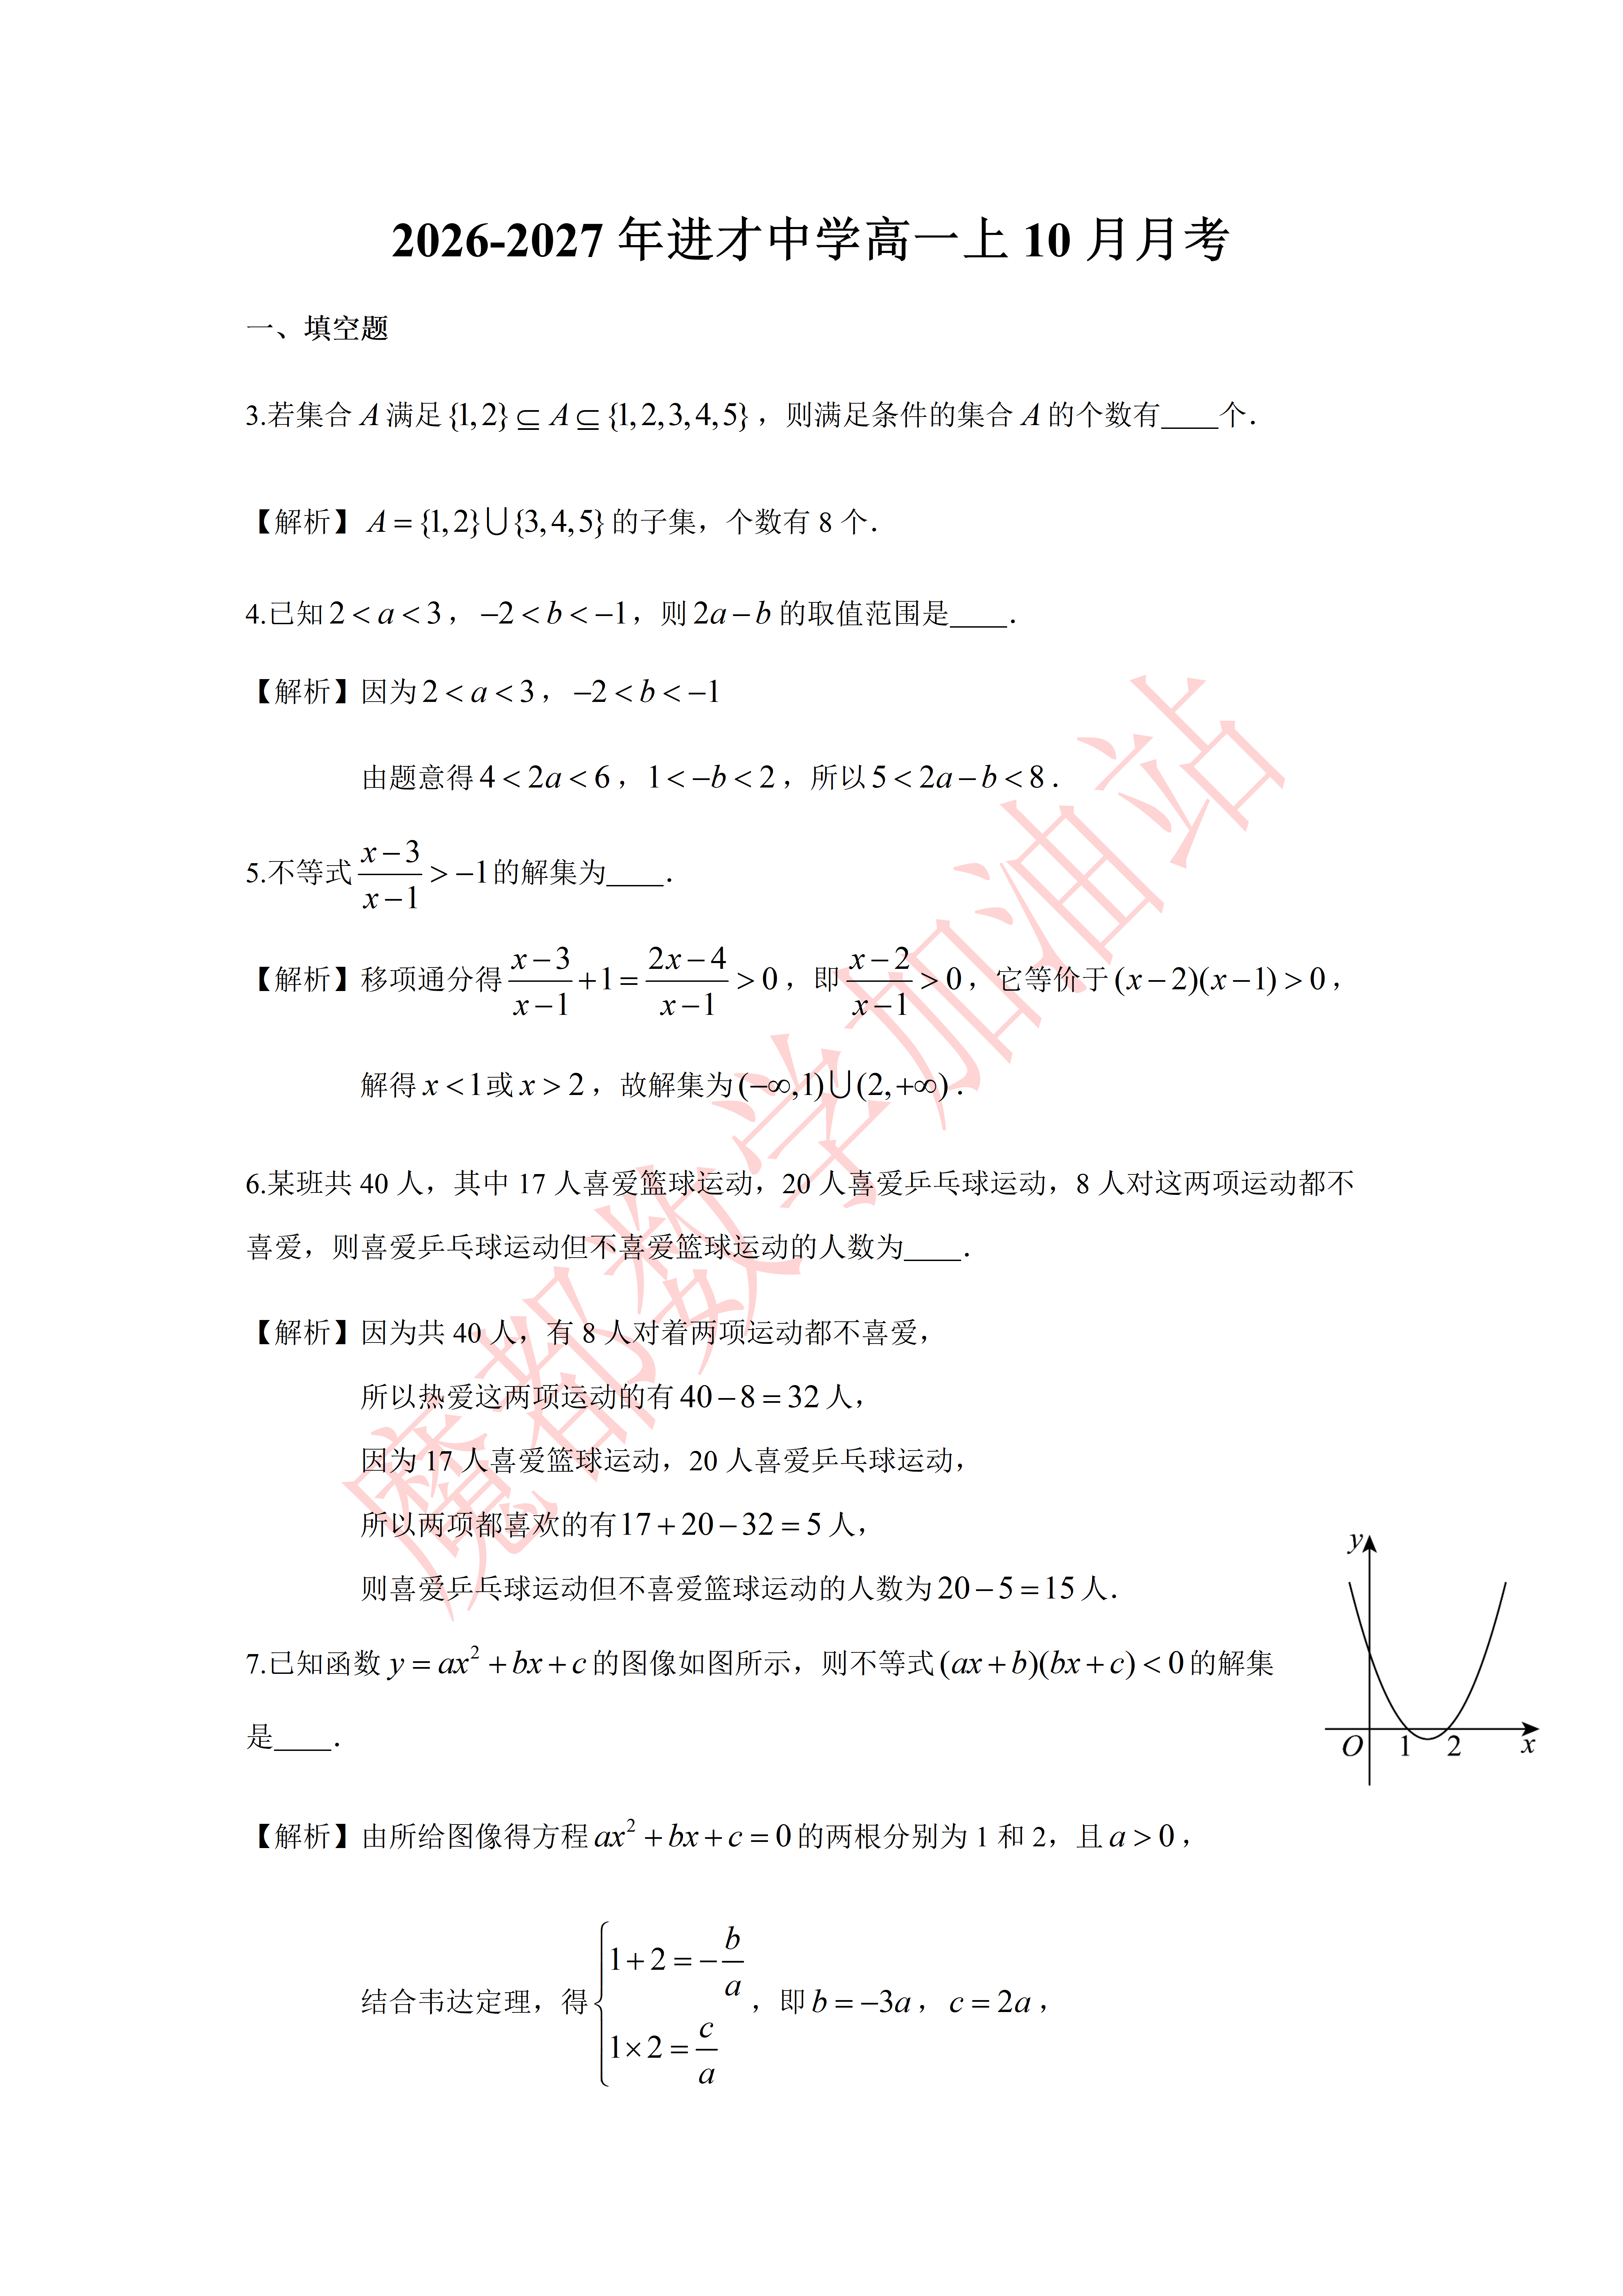
\includegraphics[width=.22\linewidth,trim=3879bp 1490bp 238bp 4492bp,clip]{../原图/高一60_进才中学_10月月考/01.png}
\end{center}

\ifanswer
\solbegin
\step{由所给图像得方程 $ax^2+bx+c=0$ 的两根分别为 1 和 2，且 $a>0$，}
\step{结合韦达定理，得 $\begin{cases}1+2=-\dfrac ba\\ 1\times2=\dfrac ca\end{cases}$，即 $b=-3a$，$c=2a$，}
\step{所以不等式 $(ax+b)(bx+c)<0$ 即 $(ax-3a)(-3ax+2a)<0$，}
\step{化简得 $(x-3)(3x-2)>0$，解得 $x<\dfrac23$ 或 $x>3$，}
\step{所以不等式 $(ax+b)(bx+c)<0$ 的解集是 $(-\infty,\dfrac23)\cup(3,+\infty)$.}
\solend
\fi

\item 已知集合 $A=\{x\mid ax=6\}$，满足 $A\subseteq\Z$，则整数 $a$ 的所有可能取值有\blankline[4.4em]个.

\ifanswer
\solbegin
\step{当 $a=0$ 时，$A=\varnothing$，而 $\varnothing\subseteq\Z$，满足题意，}
\step{当 $a\neq0$ 时，$A=\left\{\dfrac6a\right\}$，要使 $A\subseteq\Z$，则 $\dfrac6a\in\Z$，所以 $a=\pm1,\pm2,\pm3,\pm6$，}
\step{综上，整数 $a$ 的可能取值为 0，$\pm1$，$\pm2$，$\pm3$，$\pm6$，共 9 个.}
\solend
\fi

\item 设关于 $x$ 的方程 $x^2+kx+n=0$ 有两个不同实根 $x_1$、$x_2$，且 $\dfrac1{x_1}+\dfrac1{x_2}=2$，则实数 $n$ 的取值范围是\blankline[4.4em].

\ifanswer
\solbegin
\step{由于方程 $x^2+kx+n=0$ 有两个不同实根 $x_1$、$x_2$，}
\step{因此 $\Delta=k^2-4n>0$，$x_1+x_2=-k$，$x_1x_2=n$，}
\step{由 $\dfrac1{x_1}+\dfrac1{x_2}=\dfrac{x_1+x_2}{x_1x_2}=\dfrac{-k}{n}=2$，得 $k=-2n$，}
\step{因此 $\Delta=k^2-4n=4n^2-4n>0$，解得 $n<0$ 或 $n>1$，}
\step{则实数 $n$ 的取值范围是 $(-\infty,0)\cup(1,+\infty)$.}
\solend
\fi

\item 某船从甲地沿河顺流航行 $75\mathrm{km}$，到达乙码头，停留 $30\mathrm{min}$ 后再逆流航行 $126\mathrm{km}$ 到达丙地，若水流速度为 $4\mathrm{km/h}$，且该船要在 $5\mathrm{h}$ 内完成航行任务，那么船的速度至少达到\blankline[4.4em]$\mathrm{km/h}$.

\ifanswer
\solbegin
\step{设该轮船在静水中的速度是 $x$ 千米/小时，水流速度是 4 千米/小时，}
\step{由题意得 $\dfrac{75}{4+x}+0.5+\dfrac{126}{x-4}\leqslant5$，即 $9x^2-402x-552\geqslant0$，解得 $x\geqslant46$，}
\step{答：该船的速度至少是 46 千米/小时.}
\solend
\fi

\item 设实数 $a,b,c$ 满足 $a^2+b^2\leqslant c<1$，则 $a+\dfrac12b+c$ 的最小值为\blankline[4.4em].

\ifanswer
\solbegin
\step{因为 $c\geqslant a^2+b^2$，}
\step{所以 $a+\dfrac12b+c\geqslant a+\dfrac12b+a^2+b^2=\left(a+\dfrac12\right)^2+\left(b+\dfrac14\right)^2-\dfrac5{16}\geqslant-\dfrac5{16}$，}
\step{当 $a=-\dfrac12,b=-\dfrac14,c=a^2+b^2=\dfrac5{16}$（此时 $c<1$ 成立）时取到等号，}
\step{故最小值为 $-\dfrac5{16}$.}
\solend
\fi

\item 已知集合 $A=\{x\in\N^*\mid1\leqslant x\leqslant2026\}$. 设集合 $B=\{b_1,b_2,b_3,\cdots,b_n\}$ 满足 $B\subseteq A$，且对任意的 $b_i$、$b_j$、$b_k\in B(i$、$j$、$k\in\{1,2,3,\cdots,n\})$，存在 $m\in\N^*$，使得 $b_i+b_j+b_k=39m$，则 $n$ 的最大值为\blankline[4.4em].

\ifanswer
\solbegin
\step{因为 $39=1\times39=3\times13$，所以 $n$ 的最大值大于 3，}
\step{若对任意的 $b_i$、$b_j$、$b_k\in B$，存在 $m\in\N^*$，使得 $b_i+b_j+b_k=39m$，}
\step{则集合 $B$ 的元素除以 39 的余数均为 0 或均为 13 或均为 26，}
\step{即 $B=\{39,78,\cdots,39n\}$ 或 $B=\{13,52,\cdots,39n-26\}$}
\step{或 $B=\{26,65,\cdots,39n-13\}$，}
\step{若 $B=\{39,78,\cdots,39n\}$，则 $39n\leqslant2026$，}
\step{解得 $n\leqslant\dfrac{2026}{39}\in(51,52)$，此时 $n$ 的最大值为 51；}
\step{若 $B=\{13,52,\cdots,39n-26\}$，则 $39n-26\leqslant2026$，}
\step{解得 $n\leqslant\dfrac{684}{13}\in(52,53)$，此时 $n$ 的最大值为 52；}
\step{若 $B=\{26,65,\cdots,39n-13\}$，则 $39n-13\leqslant2026$，}
\step{解得 $n\leqslant\dfrac{2039}{39}\in(52,53)$，此时 $n$ 的最大值为 52；}
\step{综上，$n$ 的最大值为 52.}
\solend
\fi

\end{enumerate}

\bigsec{二、选择题}

\begin{enumerate}
\setcounter{enumi}{12}

% 第 13 题原卷无【答案】/【解析】段，答案“B”直接印在题干括号内，
% 按 高一53 第 13 题的成例括号留空、答案另提为 \ans{}（见文件头）
\item 已知 $a$、$b\in\R$，则“$|a|>|b|$”是“$a>|b|$”的\mbox{（\quad）}

\keepwithprev
A. 充分不必要条件\qquad B. 必要不充分条件

C. 充要条件\qquad D. 既不充分也不必要条件

\ifanswer
\ans{$B$}
\fi

\item 如果关于 $x$ 的一元二次方程 $x^2+2mx+(m+2)=0$ 有一正根一负根，那么 $m$ 的取值范围为\mbox{（\quad）}

\keepwithprev
A. $(-2,-1)$\qquad B. $(-1,2)$

C. $(-\infty,-1)\cup(2,+\infty)$\qquad D. $(-\infty,-2)$

\ifanswer
\solbegin
\step{设两根为 $x_1,x_2$，方程有一正根一负根，则 $\begin{cases}x_1x_2=m+2<0\\ \Delta=4m^2-4(m+2)>0\end{cases}$，}
\step{解得 $m<-2$，故选 $D$.}
\solend
\fi

\item 若不等式 $|3x-a|\leqslant x+2$ 的解集包含集合 $[0,1]$，则实数 $a$ 的取值范围为\mbox{（\quad）}

\keepwithprev
A. $[0,2]$\qquad B. $[0,1]$

C. $[1,2]$\qquad D. $(1,2)$

\ifanswer
\solbegin
% 原卷“法一：”“法二：”排红色加粗（全卷唯一红字），本稿按全稿子题标号样式排 \stepm
% （详见文件头“与原卷的排版差异”⑦）
\stepm{法一：}{不等式 $|3x-a|\leqslant x+2$ 化为 $2x-2\leqslant a\leqslant4x+2$，}
% 原卷此句缺动词（疑漏“对”字），照录未改（见文件头“原卷存疑”④）
\step{$[0,1]$ 使 $2x-2\leqslant a\leqslant4x+2$ 成立，则 $0\leqslant a\leqslant2$，故选 $A$.}
\stepm{法二：}{将两边平方整理得 $8x^2-(6a+4)x+a^2-4\leqslant0$ 对 $[0,1]$ 恒成立，}
\step{则有 $\begin{cases}a^2-4\leqslant0\\ a^2-6a\leqslant0\end{cases}$，解得 $0\leqslant a\leqslant2$，故选 $A$.}
\solend
\fi

\item 数学组 Y 老师在白纸上写下以下四个命题：

①这四个命题中至少有一个是真的；②这四个命题中至少有两个是真的；

③这四个命题中至少有两个是假的；④这四个命题中至少有一个是假的；

每个命题非真即假. 问 Y 老师在纸上写的假命题有几个？\mbox{（\quad）}

\keepwithprev
A. 0\qquad B. 1

C. 2\qquad D. 3

\ifanswer
\solbegin
\step{设四个命题中真命题的个数为 $t$，则①真 $\iff t\geqslant1$，②真 $\iff t\geqslant2$，}
\step{③真 $\iff t\leqslant2$，④真 $\iff t\leqslant3$.}
\step{逐一检验：$t=0$ 时③④为真，应为 $t=2$，矛盾；}
\step{$t=1$ 时①③④为真，应为 $t=3$，矛盾；}
\step{$t=2$ 时四个命题全为真，应为 $t=4$，矛盾；}
\step{$t=3$ 时①②④为真、③为假，恰有 3 个真命题，符合；}
\step{$t=4$ 时①②为真，应为 $t=2$，矛盾.}
\step{所以恰有 1 个假命题，故选 $B$.}
\solend
\fi

\end{enumerate}

\bigsec{三、解答题}

\begin{enumerate}
\setcounter{enumi}{16}

\item 已知：$x\in\R$，$a=x^2-1$，$b=4x+5$. 求证：$a$、$b$ 中至少有一个大于等于 0.

\ifanswer
\solbegin
\step{假设 $a$、$b$ 都小于 0，即 $a<0$，$b<0$，则 $a+b<0$.}
\step{又 $a+b=x^2-1+4x+5=x^2+4x+4=(x+2)^2\geqslant0$，}
\step{这与假设所得 $a+b<0$ 矛盾，故假设不成立，}
\step{所以 $a$、$b$ 中至少有一个大于等于 0.}
\solend
\fi

\ansspace[6]

% 原卷 A、B 两个集合定义之间排半角逗号“,”（5 倍放大核，右侧字距 19px，与全卷全角“，”的 65—79px 字距判然有别）；
% 本稿原误抄为全角“，”——已照录原卷半角（见文件头“与原卷的排版差异”⑤）
\item 已知集合 $A=\{x\mid4\leqslant x\leqslant12\}$,$B=\{x\mid a\leqslant x\leqslant2a+1\}$.

（1）若 $a=2$，求 $\overline A\cap B$；

（2）已知 $A\cup B=A$，求实数 $a$ 的取值范围.

\ifanswer
\solbegin
\stepm{(1)}{当 $a=2$ 时，$B=\{x\mid2\leqslant x\leqslant5\}$，}
\step{而 $A=\{x\mid4\leqslant x\leqslant12\}$，则 $\overline A=(-\infty,4)\cup(12,+\infty)$，所以 $\overline A\cap B=[2,4)$.}
\stepm{(2)}{$A\cup B=A$ 即 $B\subseteq A$.}
\stepm{①}{当 $B=\varnothing$ 时，$a>2a+1$，即 $a<-1$，符合；}
\stepm{②}{当 $B\neq\varnothing$ 时，需 $a\leqslant2a+1$ 且 $a\geqslant4$ 且 $2a+1\leqslant12$，即 $4\leqslant a\leqslant\dfrac{11}2$.}
\step{综上，$a$ 的取值范围是 $(-\infty,-1)\cup\left[4,\dfrac{11}2\right]$.}
\solend
\fi

\ansspace[8]

\item （1）若关于 $x$ 的不等式 $ax^2-3x+2<0$ 的解集不是空集，求实数 $a$ 的取值范围；

（2）求关于 $x$ 的不等式 $ax^2-3x+2>ax-1$ 的解集.

\ifanswer
\solbegin
\stepm{(1)}{若 $a>0$，关于 $x$ 的不等式 $ax^2-3x+2<0$ 的解集不空，}
\step{所以一元二次方程 $ax^2-3x+2=0$ 的判别式大于零，}
\step{即 $(-3)^2-8a>0\Rightarrow a<\dfrac98$，结合 $a>0$ 得 $0<a<\dfrac98$；}
\step{若 $a\leqslant0$，则关于 $x$ 的不等式 $ax^2-3x+2<0$ 的解集不是空集；}
\step{综上，实数 $a$ 的取值范围是 $\left(-\infty,\dfrac98\right)$.}
\stepm{(2)}{$ax^2-3x+2>ax-1\Rightarrow ax^2-(a+3)x+3>0\Rightarrow(ax-3)(x-1)>0$，}
\step{当 $a=0$ 时，不等式为 $x-1<0$，不等式的解集为 $\{x\mid x<1\}$；}
\step{当 $a<0$ 时，不等式化为 $\left(x-\dfrac3a\right)(x-1)<0$，}
\step{不等式的解集为 $\left\{x\mid\dfrac3a<x<1\right\}$，}
\step{当 $a>0$ 时，方程 $ax^2-3x+2=ax-1$ 的两个根分别为：$\dfrac3a,1$.}
\step{当 $a=3$ 时，两根相等，故不等式的解集为 $\{x\mid x\neq1\}$；}
\step{当 $a>3$ 时，$\dfrac3a<1$，不等式的解集为 $\left\{x\mid x<\dfrac3a\right.$ 或 $\left.x>1\right\}$；}
\step{当 $0<a<3$ 时，$\dfrac3a>1$，不等式的解集为 $\left\{x\mid x<1\right.$ 或 $\left.x>\dfrac3a\right\}$；}
\step{综上所述，当 $a<0$ 时，不等式的解集为 $\left\{x\mid\dfrac3a<x<1\right\}$，}
\step{当 $a=0$ 时，不等式的解集为 $\{x\mid x<1\}$，}
\step{当 $0<a<3$ 时，不等式的解集为 $\left\{x\mid x<1\right.$ 或 $\left.x>\dfrac3a\right\}$，}
\step{当 $a=3$ 时，不等式的解集为 $\{x\mid x\neq1\}$，}
\step{当 $a>3$ 时，不等式的解集为 $\left\{x\mid x<\dfrac3a\right.$ 或 $\left.x>1\right\}$.}
\solend
\fi

\ansspace[8]

\item 设命题 $p$：对任意 $x\in\R$，使得不等式 $mx^2-mx+2>0$ 恒成立；命题 $q$：存在 $0\leqslant x\leqslant3$，不等式 $2x-2\geqslant|m|$ 成立.

（1）若 $p$ 为真命题，求实数 $m$ 的取值范围；

（2）若 $p$、$q$ 有且只有一个是真命题，求实数 $m$ 的取值范围.

\ifanswer
\solbegin
\stepm{(1)}{因为 $p:\forall x\in\R$，$mx^2-mx+2>0$ 为真命题，}
\step{所以当 $m=0$ 时，不等式为 $2>0$，在 $\R$ 上恒成立，符合题意；}
\step{当 $m\neq0$ 时，$\begin{cases}m>0\\ \Delta=m^2-8m<0\end{cases}$，解得 $0<m<8$.}
\step{综上，实数 $m$ 的取值范围为 $[0,8)$.}
\stepm{(2)}{若 $q$ 为真命题，即 $q:\exists0\leqslant x\leqslant3$，$2x-2\geqslant|m|$，}
\step{则对于 $0\leqslant x\leqslant3$，$(2x-2)_{max}\geqslant|m|$.}
\step{由于 $0\leqslant x\leqslant3$，$2x-2\in[-2,4]$，所以 $|m|\leqslant4$，解得 $-4\leqslant m\leqslant4$，}
\step{又因为 $p$、$q$ 有且只有一个是真命题，}
\step{所以当 $p$ 真 $q$ 假时，$\begin{cases}0\leqslant m<8\\ m<-4\text{或}m>4\end{cases}$，解得 $4<m<8$；}
\step{当 $p$ 假 $q$ 真时，$\begin{cases}m<0\text{或}m\geqslant8\\ -4\leqslant m\leqslant4\end{cases}$，解得 $-4\leqslant m<0$；}
\step{综上，实数 $m$ 的取值范围为 $[-4,0)\cup(4,8)$.}
\solend
\fi

\ansspace[10]

\item 已知集合 $A=\{a_1,a_2,\cdots,a_k\}(k\geqslant2)$. 其中 $a_i\in\N^*(i=1,2,\cdots,k)$. 若对于任意的 $a\in A$，总有 $\dfrac1a\notin A$，则称集合 $A$ 具有性质 $P$. 由 $A$ 中的元素构成两个相应的集合：$S=\{(a,b)\mid a\in A,b\in A,ab\in A\}$，$T=\left\{(a,b)\mid a\in A,b\in A,\dfrac ab\in A\right\}$，其中 $(a,b)$ 是有序数对，集合 $S$ 和 $T$ 中的元素个数分别为 $m$ 和 $n$.

（1）检验集合 $\{2,3,6\}$ 与 $\{1,2,4\}$ 是否具有性质 $P$，并对其中具有性质 $P$ 的集合，写出相应的集合 $S$ 和 $T$；

（2）对任何具有性质 $P$ 的集合 $A$，$n$ 的最大值为多少？（直接写出答案，无需说明理由）；

% 原卷题干的小问编号跳号：印作 (1)(2)(4)，本稿照录 (4)、未改成 (3)（见文件头“原卷存疑”①）
（4）判断 $m$ 和 $n$ 的大小关系，并证明你的结论.

\ifanswer
\solbegin
\stepm{(1)}{因为 $\dfrac12\in\{1,2,4\}$，所以 $\{1,2,4\}$ 不具有性质 $P$；}
\step{因为 $\dfrac12\notin\{2,3,6\}$，$\dfrac13\notin\{2,3,6\}$，$\dfrac16\notin\{2,3,6\}$，所以 $\{2,3,6\}$ 具有性质 $P$.}
\step{$S=\{(2,3),(3,2)\}$，$T=\{(6,2),(6,3)\}$；}
\stepm{(2)}{因为对于任意的 $a\in A$，总有 $\dfrac1a\notin A$，所以 $1\notin A$，}
% 原卷此处印作“$\{(a_i,a_i)\}\in T$”，与上一句“$1\notin A$”及下文“最多为 $C_k^2$”的推理
% 均不自洽（应为“$\notin$”），已 8 倍放大确认无斜线；照录未改（见文件头“原卷存疑”③）
\step{从而 $\{(a_i,a_i)\}\in T(i=1,2,\cdots,k)$.}
\step{因为 $a\in A,b\in A,\dfrac ab\in A$，所以当 $i\neq j$ 时，}
\step{$(a_i,a_j)\in T$ 和 $(a_j,a_i)\in T(i,j=1,2,\cdots,k)$ 至多有一个成立，}
\step{所以集合 $T$ 中的元素个数最多为 $C_k^2=\dfrac{k(k-1)}2$，即 $n\leqslant\dfrac{k(k-1)}2$.}
% 原卷【解析】把第 (4) 问标作“(3)”（与题干跳号相应），本稿照录未改（见文件头“原卷存疑”①）
\stepm{(3)}{$m=n$，证明如下：}
\step{①设 $(a,b)\in T$，则 $a\in A,b\in A,\dfrac ab\in A$. 设 $c=\dfrac ab$，则 $a=bc$，}
\step{故 $b\in A$，$c\in A$，$bc\in A$，从而 $(b,c)\in S$，}
\step{即对 $\forall(a,b)\in T$，总 $\exists c$ 使 $(b,c)\in S$，从而 $n\leqslant m$.}
\step{②设 $(p,q)\in S$，则 $p\in A$，$q\in A$，$pq\in A$.}
\step{设 $r=pq$，则 $q=\dfrac rp$，故 $r\in A,p\in A,\dfrac rp\in A$，从而 $(r,p)\in T$，}
\step{即对 $\forall(p,q)\in S$，总 $\exists r$ 使 $(r,p)\in T$，从而 $m\leqslant n$.}
\step{由①②得 $m=n$.}
\solend
\fi

\ansspace*[10]

\end{enumerate}

\end{document}
